% Options for packages loaded elsewhere
% Options for packages loaded elsewhere
\PassOptionsToPackage{unicode}{hyperref}
\PassOptionsToPackage{hyphens}{url}
\PassOptionsToPackage{dvipsnames,svgnames,x11names}{xcolor}
%
\documentclass[
  letterpaper,
  DIV=11,
  numbers=noendperiod,
  oneside]{scrreprt}
\usepackage{xcolor}
\usepackage[left=1in,marginparwidth=2.0666666666667in,textwidth=4.1333333333333in,marginparsep=0.3in]{geometry}
\usepackage{amsmath,amssymb}
\setcounter{secnumdepth}{5}
\usepackage{iftex}
\ifPDFTeX
  \usepackage[T1]{fontenc}
  \usepackage[utf8]{inputenc}
  \usepackage{textcomp} % provide euro and other symbols
\else % if luatex or xetex
  \usepackage{unicode-math} % this also loads fontspec
  \defaultfontfeatures{Scale=MatchLowercase}
  \defaultfontfeatures[\rmfamily]{Ligatures=TeX,Scale=1}
\fi
\usepackage{lmodern}
\ifPDFTeX\else
  % xetex/luatex font selection
\fi
% Use upquote if available, for straight quotes in verbatim environments
\IfFileExists{upquote.sty}{\usepackage{upquote}}{}
\IfFileExists{microtype.sty}{% use microtype if available
  \usepackage[]{microtype}
  \UseMicrotypeSet[protrusion]{basicmath} % disable protrusion for tt fonts
}{}
\makeatletter
\@ifundefined{KOMAClassName}{% if non-KOMA class
  \IfFileExists{parskip.sty}{%
    \usepackage{parskip}
  }{% else
    \setlength{\parindent}{0pt}
    \setlength{\parskip}{6pt plus 2pt minus 1pt}}
}{% if KOMA class
  \KOMAoptions{parskip=half}}
\makeatother
% Make \paragraph and \subparagraph free-standing
\makeatletter
\ifx\paragraph\undefined\else
  \let\oldparagraph\paragraph
  \renewcommand{\paragraph}{
    \@ifstar
      \xxxParagraphStar
      \xxxParagraphNoStar
  }
  \newcommand{\xxxParagraphStar}[1]{\oldparagraph*{#1}\mbox{}}
  \newcommand{\xxxParagraphNoStar}[1]{\oldparagraph{#1}\mbox{}}
\fi
\ifx\subparagraph\undefined\else
  \let\oldsubparagraph\subparagraph
  \renewcommand{\subparagraph}{
    \@ifstar
      \xxxSubParagraphStar
      \xxxSubParagraphNoStar
  }
  \newcommand{\xxxSubParagraphStar}[1]{\oldsubparagraph*{#1}\mbox{}}
  \newcommand{\xxxSubParagraphNoStar}[1]{\oldsubparagraph{#1}\mbox{}}
\fi
\makeatother
\usepackage{color}
\usepackage{fancyvrb}
\newcommand{\VerbBar}{|}
\newcommand{\VERB}{\Verb[commandchars=\\\{\}]}
\DefineVerbatimEnvironment{Highlighting}{Verbatim}{commandchars=\\\{\}}
% Add ',fontsize=\small' for more characters per line
\usepackage{framed}
\definecolor{shadecolor}{RGB}{241,243,245}
\newenvironment{Shaded}{\begin{snugshade}}{\end{snugshade}}
\newcommand{\AlertTok}[1]{\textcolor[rgb]{0.68,0.00,0.00}{#1}}
\newcommand{\AnnotationTok}[1]{\textcolor[rgb]{0.37,0.37,0.37}{#1}}
\newcommand{\AttributeTok}[1]{\textcolor[rgb]{0.40,0.45,0.13}{#1}}
\newcommand{\BaseNTok}[1]{\textcolor[rgb]{0.68,0.00,0.00}{#1}}
\newcommand{\BuiltInTok}[1]{\textcolor[rgb]{0.00,0.23,0.31}{#1}}
\newcommand{\CharTok}[1]{\textcolor[rgb]{0.13,0.47,0.30}{#1}}
\newcommand{\CommentTok}[1]{\textcolor[rgb]{0.37,0.37,0.37}{#1}}
\newcommand{\CommentVarTok}[1]{\textcolor[rgb]{0.37,0.37,0.37}{\textit{#1}}}
\newcommand{\ConstantTok}[1]{\textcolor[rgb]{0.56,0.35,0.01}{#1}}
\newcommand{\ControlFlowTok}[1]{\textcolor[rgb]{0.00,0.23,0.31}{\textbf{#1}}}
\newcommand{\DataTypeTok}[1]{\textcolor[rgb]{0.68,0.00,0.00}{#1}}
\newcommand{\DecValTok}[1]{\textcolor[rgb]{0.68,0.00,0.00}{#1}}
\newcommand{\DocumentationTok}[1]{\textcolor[rgb]{0.37,0.37,0.37}{\textit{#1}}}
\newcommand{\ErrorTok}[1]{\textcolor[rgb]{0.68,0.00,0.00}{#1}}
\newcommand{\ExtensionTok}[1]{\textcolor[rgb]{0.00,0.23,0.31}{#1}}
\newcommand{\FloatTok}[1]{\textcolor[rgb]{0.68,0.00,0.00}{#1}}
\newcommand{\FunctionTok}[1]{\textcolor[rgb]{0.28,0.35,0.67}{#1}}
\newcommand{\ImportTok}[1]{\textcolor[rgb]{0.00,0.46,0.62}{#1}}
\newcommand{\InformationTok}[1]{\textcolor[rgb]{0.37,0.37,0.37}{#1}}
\newcommand{\KeywordTok}[1]{\textcolor[rgb]{0.00,0.23,0.31}{\textbf{#1}}}
\newcommand{\NormalTok}[1]{\textcolor[rgb]{0.00,0.23,0.31}{#1}}
\newcommand{\OperatorTok}[1]{\textcolor[rgb]{0.37,0.37,0.37}{#1}}
\newcommand{\OtherTok}[1]{\textcolor[rgb]{0.00,0.23,0.31}{#1}}
\newcommand{\PreprocessorTok}[1]{\textcolor[rgb]{0.68,0.00,0.00}{#1}}
\newcommand{\RegionMarkerTok}[1]{\textcolor[rgb]{0.00,0.23,0.31}{#1}}
\newcommand{\SpecialCharTok}[1]{\textcolor[rgb]{0.37,0.37,0.37}{#1}}
\newcommand{\SpecialStringTok}[1]{\textcolor[rgb]{0.13,0.47,0.30}{#1}}
\newcommand{\StringTok}[1]{\textcolor[rgb]{0.13,0.47,0.30}{#1}}
\newcommand{\VariableTok}[1]{\textcolor[rgb]{0.07,0.07,0.07}{#1}}
\newcommand{\VerbatimStringTok}[1]{\textcolor[rgb]{0.13,0.47,0.30}{#1}}
\newcommand{\WarningTok}[1]{\textcolor[rgb]{0.37,0.37,0.37}{\textit{#1}}}
\usepackage{longtable,booktabs,array}
\usepackage{calc} % for calculating minipage widths
% Correct order of tables after \paragraph or \subparagraph
\usepackage{etoolbox}
\makeatletter
\patchcmd\longtable{\par}{\if@noskipsec\mbox{}\fi\par}{}{}
\makeatother
% Allow footnotes in longtable head/foot
\IfFileExists{footnotehyper.sty}{\usepackage{footnotehyper}}{\usepackage{footnote}}
\makesavenoteenv{longtable}
\usepackage{graphicx}
\makeatletter
\newsavebox\pandoc@box
\newcommand*\pandocbounded[1]{% scales image to fit in text height/width
  \sbox\pandoc@box{#1}%
  \Gscale@div\@tempa{\textheight}{\dimexpr\ht\pandoc@box+\dp\pandoc@box\relax}%
  \Gscale@div\@tempb{\linewidth}{\wd\pandoc@box}%
  \ifdim\@tempb\p@<\@tempa\p@\let\@tempa\@tempb\fi% select the smaller of both
  \ifdim\@tempa\p@<\p@\scalebox{\@tempa}{\usebox\pandoc@box}%
  \else\usebox{\pandoc@box}%
  \fi%
}
% Set default figure placement to htbp
\def\fps@figure{htbp}
\makeatother
\setlength{\emergencystretch}{3em} % prevent overfull lines
\providecommand{\tightlist}{%
  \setlength{\itemsep}{0pt}\setlength{\parskip}{0pt}}
\usepackage{bookmark}
\IfFileExists{xurl.sty}{\usepackage{xurl}}{} % add URL line breaks if available
\urlstyle{same}
\hypersetup{
  pdftitle={ESIIL Learning Portal},
  pdfauthor={ESIIL Education},
  colorlinks=true,
  linkcolor={blue},
  filecolor={Maroon},
  citecolor={Blue},
  urlcolor={Blue},
  pdfcreator={LaTeX via pandoc}}


\title{ESIIL Learning Portal}
\author{ESIIL Education}
\date{2025-08-15}
\begin{document}
\maketitle


\bookmarksetup{startatroot}

\chapter{Welcome to the ESIIL Learning
Portal!}\label{welcome-to-the-esiil-learning-portal}

\href{./index.html?show-results=1}{\pandocbounded{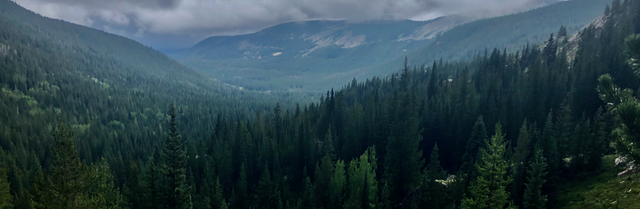
\includegraphics[keepaspectratio]{img/search.png}}}

Explore textbooks:

\begin{itemize}
\tightlist
\item
  \href{pages/00-overviews/04a-courses/foundations/index.html}{Introduction
  to Earth Data Science}
\item
  \href{pages/00-overviews/04a-courses/shortcourse/index.html}{ESIIL
  Data Short Course}
\item
  \href{pages/00-overviews/04a-courses/stars/index.html}{ESIIL STARS
  Textbook}
\end{itemize}

Explore collaborative workshops:

\begin{itemize}
\tightlist
\item
  \href{https://earthdatascience.org/pages/00-overviews/04b-events/esa25/}{ESA
  PhenoCam 2025 Workshop}
\end{itemize}

\bookmarksetup{startatroot}

\chapter{The Midwest underwater}\label{the-midwest-underwater}

A look at 2019 floods in South Dakota, USA

\hfill\break

\begin{figure}[H]

{\centering \pandocbounded{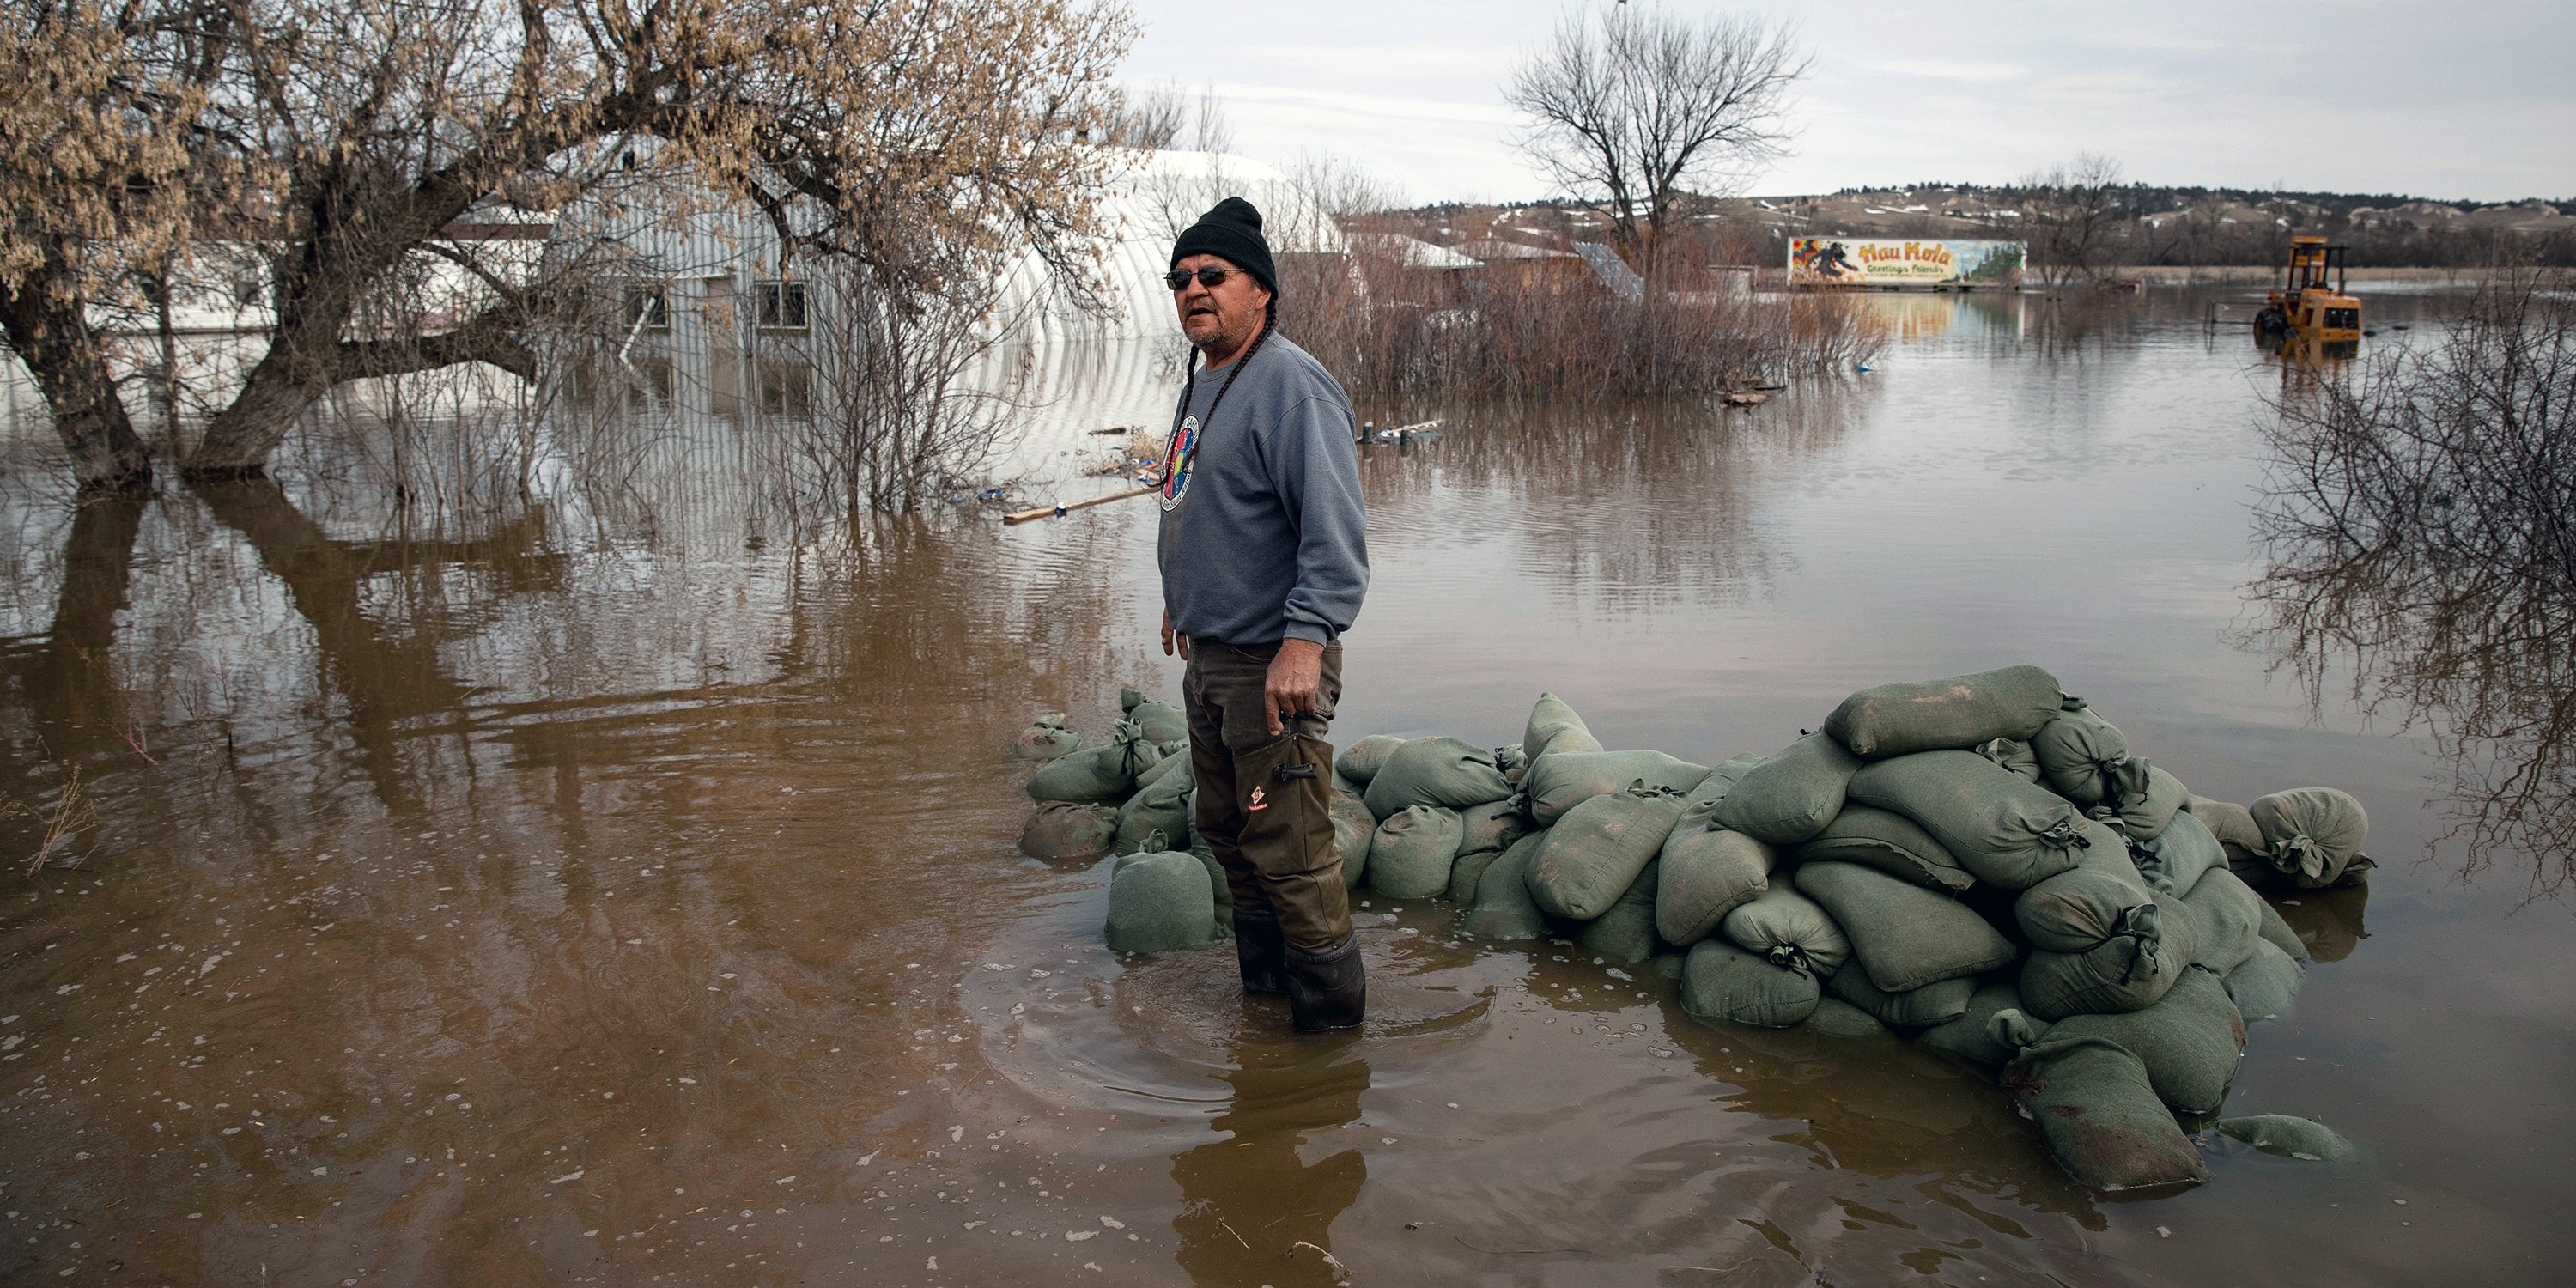
\includegraphics[keepaspectratio]{img/earth-analytics/flood-frequency/pipeline-flooding.jpg}}

}

\caption{Image source:
\href{https://theintercept.com/2019/04/05/keystone-xl-pipeline-pine-ridge-floods}{The
Intercept April 5, 2019}}

\end{figure}%

\begin{tcolorbox}[enhanced jigsaw, colbacktitle=quarto-callout-color!10!white, opacityback=0, bottomtitle=1mm, toptitle=1mm, bottomrule=.15mm, left=2mm, colframe=quarto-callout-color-frame, leftrule=.75mm, opacitybacktitle=0.6, colback=white, rightrule=.15mm, toprule=.15mm, breakable, titlerule=0mm, title=\textcolor{quarto-callout-color}{\faInfo}\hspace{0.5em}{Read More}, coltitle=black, arc=.35mm]

Check out what some US government and news sources said about the floods
in 2019. Here are some resources from different sources to get you
started:

\begin{itemize}
\tightlist
\item
  \href{https://www.weather.gov/fsd/20190314-Flooding}{The National
  Weather Service}
\item
  \href{https://theintercept.com/2019/04/05/keystone-xl-pipeline-pine-ridge-floods/}{The
  Intercept}
\item
  \href{https://yaleclimateconnections.org/2019/04/did-climate-change-cause-midwest-flooding/}{Yale
  Climate Connections}
\item
  \href{https://www.sdpb.org/news/2019-10-17/cheyenne-river-tribe-says-oahe-dam-has-caused-problems-for-decades}{South
  Dakota Public Radio}
\end{itemize}

If you know someone who lived through these or similar floods, we also
invite you to ask them about that experience.

\end{tcolorbox}

\begin{tcolorbox}[enhanced jigsaw, colbacktitle=quarto-callout-color!10!white, opacityback=0, bottomtitle=1mm, toptitle=1mm, bottomrule=.15mm, left=2mm, colframe=quarto-callout-color-frame, leftrule=.75mm, opacitybacktitle=0.6, colback=white, rightrule=.15mm, toprule=.15mm, breakable, titlerule=0mm, title=\textcolor{quarto-callout-color}{\faInfo}\hspace{0.5em}{Reflect and Respond}, coltitle=black, arc=.35mm]

Based on your reading and conversations, what do you think some of the
causes of the 2019 flooding in South Dakota were?

\end{tcolorbox}

We like to keep important values up at the top of the notebook -- it
makes them easy to modify. You can use the following cell to change
parameters about your workflow if you like:

\begin{Shaded}
\begin{Highlighting}[]
\BuiltInTok{id} \OperatorTok{=} \StringTok{\textquotesingle{}stars\textquotesingle{}}
\NormalTok{site\_name }\OperatorTok{=} \StringTok{\textquotesingle{}Cheyenne River near Wasta\textquotesingle{}}
\NormalTok{year }\OperatorTok{=} \DecValTok{2019}
\NormalTok{project\_title }\OperatorTok{=} \StringTok{\textquotesingle{}Cheyenne River Flood Frequency\textquotesingle{}}
\NormalTok{project\_dirname }\OperatorTok{=} \StringTok{\textquotesingle{}flood{-}cheyenne\textquotesingle{}}
\end{Highlighting}
\end{Shaded}

\bookmarksetup{startatroot}

\chapter{Access streamflow data}\label{access-streamflow-data}

One way to express how big a flood is by estimating how often larger
floods occur. For example, you might have heard news media talking about
a ``100-year flood''.

In this notebook, you will write Python code to download and work with a
\textbf{time series} of streamflow data during the flooding on the
Cheyenne River.

\begin{tcolorbox}[enhanced jigsaw, colbacktitle=quarto-callout-tip-color!10!white, opacityback=0, bottomtitle=1mm, toptitle=1mm, bottomrule=.15mm, left=2mm, colframe=quarto-callout-tip-color-frame, leftrule=.75mm, opacitybacktitle=0.6, colback=white, rightrule=.15mm, toprule=.15mm, breakable, titlerule=0mm, title=\textcolor{quarto-callout-tip-color}{\faLightbulb}\hspace{0.5em}{Tip}, coltitle=black, arc=.35mm]

A \textbf{time series} of data is taken at the same location but
collected regularly or semi-regularly over time.

\end{tcolorbox}

You will then use the data to assess when the flooding was at it's
worst.

As an \textbf{extra challenge} you could consider how the values
compared to other years by computing the flood's \textbf{return period}.

\begin{tcolorbox}[enhanced jigsaw, colbacktitle=quarto-callout-tip-color!10!white, opacityback=0, bottomtitle=1mm, toptitle=1mm, bottomrule=.15mm, left=2mm, colframe=quarto-callout-tip-color-frame, leftrule=.75mm, opacitybacktitle=0.6, colback=white, rightrule=.15mm, toprule=.15mm, breakable, titlerule=0mm, title=\textcolor{quarto-callout-tip-color}{\faLightbulb}\hspace{0.5em}{Tip}, coltitle=black, arc=.35mm]

A \textbf{return period} is an estimate of how often you might expect to
see a flood of at least a particular size. This does \emph{NOT} mean an
extreme flood ``has'' to occur within the return period, or that it
couldn't occur more than once. However, it does allow us to assess the
probability that a sequence of floods would happen and evaluate whether
or not we need to change forecasting tools or engineering standards to
meet a new reality. For example, it would be really unusual to get three
100-year floods in a ten year period without some kind of underlying
change in the climate.

\end{tcolorbox}

\begin{tcolorbox}[enhanced jigsaw, colbacktitle=quarto-callout-color!10!white, opacityback=0, bottomtitle=1mm, toptitle=1mm, bottomrule=.15mm, left=2mm, colframe=quarto-callout-color-frame, leftrule=.75mm, opacitybacktitle=0.6, colback=white, rightrule=.15mm, toprule=.15mm, breakable, titlerule=0mm, title=\textcolor{quarto-callout-color}{\faInfo}\hspace{0.5em}{Read More}, coltitle=black, arc=.35mm]

Here are some resources from your text book you can review to learn
more:

\begin{itemize}
\tightlist
\item
  \href{https://www.earthdatascience.org/courses/use-data-open-source-python/use-time-series-data-in-python/}{Introduction
  to time-series data}
\item
  \href{https://www.earthdatascience.org/courses/use-data-open-source-python/use-time-series-data-in-python/floods-return-period-and-probability/}{Flood
  return period and probability}
\end{itemize}

\end{tcolorbox}

\begin{tcolorbox}[enhanced jigsaw, colbacktitle=quarto-callout-color!10!white, opacityback=0, bottomtitle=1mm, toptitle=1mm, bottomrule=.15mm, left=2mm, colframe=quarto-callout-color-frame, leftrule=.75mm, opacitybacktitle=0.6, colback=white, rightrule=.15mm, toprule=.15mm, breakable, titlerule=0mm, title=\textcolor{quarto-callout-color}{\faInfo}\hspace{0.5em}{Reflect and Respond}, coltitle=black, arc=.35mm]

Explain what data you will need to complete this analysis, including:

\begin{enumerate}
\def\labelenumi{\arabic{enumi}.}
\tightlist
\item
  What type or types of data do you need?
\item
  How many years of data do you think you need to compute the return
  period of an extreme event like the \textbf{?meta:params.year}
  \textbf{?meta:params.site\_name} floods?
\end{enumerate}

\end{tcolorbox}

\section{STEP 0: Get set up to use
Python}\label{step-0-get-set-up-to-use-python}

Use the cell below to add necessary \textbf{package imports} to this
notebook. It's best to import everything in your very first code cell
because it helps folks who are reading your code to figure out where
everything comes from (mostly right now this is \textbf{you} in the
future). It's \emph{very} frustrating to try to figure out what packages
need to be installed to get some code to run.

\begin{tcolorbox}[enhanced jigsaw, colbacktitle=quarto-callout-note-color!10!white, opacityback=0, bottomtitle=1mm, toptitle=1mm, bottomrule=.15mm, left=2mm, colframe=quarto-callout-note-color-frame, leftrule=.75mm, opacitybacktitle=0.6, colback=white, rightrule=.15mm, toprule=.15mm, breakable, titlerule=0mm, title=\textcolor{quarto-callout-note-color}{\faInfo}\hspace{0.5em}{Note}, coltitle=black, arc=.35mm]

Our friend \href{https://peps.python.org/pep-0008/\#imports}{the PEP-8
style guide has some things to say about imports}. In particular, your
imports should be in alphabetical order.

\end{tcolorbox}

\begin{tcolorbox}[enhanced jigsaw, colbacktitle=quarto-callout-color!10!white, opacityback=0, bottomtitle=1mm, toptitle=1mm, bottomrule=.15mm, left=2mm, colframe=quarto-callout-color-frame, leftrule=.75mm, opacitybacktitle=0.6, colback=white, rightrule=.15mm, toprule=.15mm, breakable, titlerule=0mm, title=\textcolor{quarto-callout-color}{\faInfo}\hspace{0.5em}{Try It}, coltitle=black, arc=.35mm]

In the sample code below, we've imported a library needed for working
with \textbf{tabular}, or spreadsheet, data, as well as our own library
for common Environmental Data Analytics tasks (in this case, managing
files on your computer). You will also need to:

\begin{enumerate}
\def\labelenumi{\arabic{enumi}.}
\tightlist
\item
  Add the \textbf{library for working with vector data in Python} and a
  \textbf{library for creating interactive plots of vector and
  time-series data} to the imports.
\item
  Check that your imports follow the PEP-8 guidelines -- they should be
  in alphabetical order.
\item
  Run your import cell to make sure everything will work
\end{enumerate}

\end{tcolorbox}

\begin{Shaded}
\begin{Highlighting}[]
\CommentTok{\# Import libraries}
\ImportTok{import}\NormalTok{ earthpy}
\ImportTok{import}\NormalTok{ pandas }\ImportTok{as}\NormalTok{ pd}
\end{Highlighting}
\end{Shaded}

Finally, we have arranged some sample data for you, which you can
download using the \texttt{earthpy} library. Later on, you'll learn how
to download data from the NWIS using the \texttt{dataretrieval} library.
For now, you can use the sample data downloaded with the
\texttt{earthpy} library.

\begin{tcolorbox}[enhanced jigsaw, colbacktitle=quarto-callout-color!10!white, opacityback=0, bottomtitle=1mm, toptitle=1mm, bottomrule=.15mm, left=2mm, colframe=quarto-callout-color-frame, leftrule=.75mm, opacitybacktitle=0.6, colback=white, rightrule=.15mm, toprule=.15mm, breakable, titlerule=0mm, title=\textcolor{quarto-callout-color}{\faInfo}\hspace{0.5em}{Try It}, coltitle=black, arc=.35mm]

The following code will download the sample data based on the value of
``title'', and store it in the data directory on your computer. It will
also save the path to the downloaded data. You can use the
\texttt{project} later on to do things like locate data files on the
computer or image you're using to code. You should practice writing
descriptive code by:

\begin{enumerate}
\def\labelenumi{\arabic{enumi}.}
\tightlist
\item
  Change
  \texttt{\textquotesingle{}project-folder-name\textquotesingle{}} to a
  descriptive directory name where you want to store your data.
\item
  Change \texttt{data\_path} to a descriptive variable name
\item
  Run the data download cell to make sure everything will work
\end{enumerate}

\end{tcolorbox}

\begin{Shaded}
\begin{Highlighting}[]
\CommentTok{\# Create project directory}
\NormalTok{project }\OperatorTok{=}\NormalTok{ earthpy.Project(title}\OperatorTok{=}\NormalTok{project\_title, dirname}\OperatorTok{=}\StringTok{\textquotesingle{}project{-}folder{-}name\textquotesingle{}}\NormalTok{)}
\CommentTok{\# Download data}
\NormalTok{data\_path }\OperatorTok{=}\NormalTok{ project.get\_data()}
\CommentTok{\# Display the project data directory location}
\NormalTok{project.project\_dir}
\end{Highlighting}
\end{Shaded}

You can use an open science tool called \texttt{bash} or the
\texttt{shell} to work with files and get information about your file
system. For example, this code will \textbf{list} (ls) the contents of
the project directory

\begin{Shaded}
\begin{Highlighting}[]
\OperatorTok{!}\NormalTok{ls }\StringTok{"$project.project\_dir"}
\end{Highlighting}
\end{Shaded}

\begin{verbatim}
cheyenne_streamflow_1934_2024.csv
\end{verbatim}

\begin{tcolorbox}[enhanced jigsaw, colbacktitle=quarto-callout-color!10!white, opacityback=0, bottomtitle=1mm, toptitle=1mm, bottomrule=.15mm, left=2mm, colframe=quarto-callout-color-frame, leftrule=.75mm, opacitybacktitle=0.6, colback=white, rightrule=.15mm, toprule=.15mm, breakable, titlerule=0mm, title=\textcolor{quarto-callout-color}{\faInfo}\hspace{0.5em}{Try It}, coltitle=black, arc=.35mm]

Go check to see if you can find the files using some other method!

\end{tcolorbox}

\begin{tcolorbox}[enhanced jigsaw, colbacktitle=quarto-callout-warning-color!10!white, opacityback=0, bottomtitle=1mm, toptitle=1mm, bottomrule=.15mm, left=2mm, colframe=quarto-callout-warning-color-frame, leftrule=.75mm, opacitybacktitle=0.6, colback=white, rightrule=.15mm, toprule=.15mm, breakable, titlerule=0mm, title=\textcolor{quarto-callout-warning-color}{\faExclamationTriangle}\hspace{0.5em}{Warning}, coltitle=black, arc=.35mm]

Are you working in the cloud, such as on GitHub Codespaces? Be aware
that any files you download to a cloud computer \textbf{will not be
saved} on the physical computer you are using! They will remain in the
cloud. So, you will not be able to see any downloaded files using the
File Explorer or Finder on your computer because they aren't there.

\end{tcolorbox}

\section{STEP 1: Site Description and
Map}\label{step-1-site-description-and-map}

In our example analysis, we'll be focusing on the Cheyenne River, which
flows into Lake Oahu by looking at a stream gage near Wasta, SD, USA.
After we've completed this example analysis, we suggest that you look
into another flood -- perhaps one that you have a personal connection
to.

\subsection{Site Description}\label{site-description}

\begin{tcolorbox}[enhanced jigsaw, colbacktitle=quarto-callout-color!10!white, opacityback=0, bottomtitle=1mm, toptitle=1mm, bottomrule=.15mm, left=2mm, colframe=quarto-callout-color-frame, leftrule=.75mm, opacitybacktitle=0.6, colback=white, rightrule=.15mm, toprule=.15mm, breakable, titlerule=0mm, title=\textcolor{quarto-callout-color}{\faInfo}\hspace{0.5em}{Try It}, coltitle=black, arc=.35mm]

Describe the Cheyenne River area in a few sentences. You can include:

\begin{itemize}
\tightlist
\item
  Information about the \textbf{climatology} of the area, or typical
  precipitation and temperature at different months of the year
\item
  The \textbf{runoff ratio} (average annual runoff divided by average
  annual precipitation)
\item
  Which \textbf{wildlife and ecosystems} exist in the area
\item
  What \textbf{communities and infrastructure} are in the area
\end{itemize}

\end{tcolorbox}

\subsection{Site Map: The Cheyenne River near
Wasta}\label{site-map-the-cheyenne-river-near-wasta}

The code below will create an interactive map of the area. But something
is wrong - no one defined the latitude and longitude as
\textbf{variables}. Try running the code to see what happens when you
reference a variable name that doesn't exist!

\begin{tcolorbox}[enhanced jigsaw, colbacktitle=quarto-callout-color!10!white, opacityback=0, bottomtitle=1mm, toptitle=1mm, bottomrule=.15mm, left=2mm, colframe=quarto-callout-color-frame, leftrule=.75mm, opacitybacktitle=0.6, colback=white, rightrule=.15mm, toprule=.15mm, breakable, titlerule=0mm, title=\textcolor{quarto-callout-color}{\faInfo}\hspace{0.5em}{Try It}, coltitle=black, arc=.35mm]

Find the location of the Cheyenne River near Wasta \textbf{USGS stream
gauge} using the \href{https://waterdata.usgs.gov/nwis?}{National Water
Information System}. This is not the easiest thing to find if you aren't
used to NWIS, so we've provided some screenshots of the process below.

\end{tcolorbox}

\paragraph{Step 1: NWIS Mapper}\label{step-1-nwis-mapper}

\begin{figure}[H]

{\centering \pandocbounded{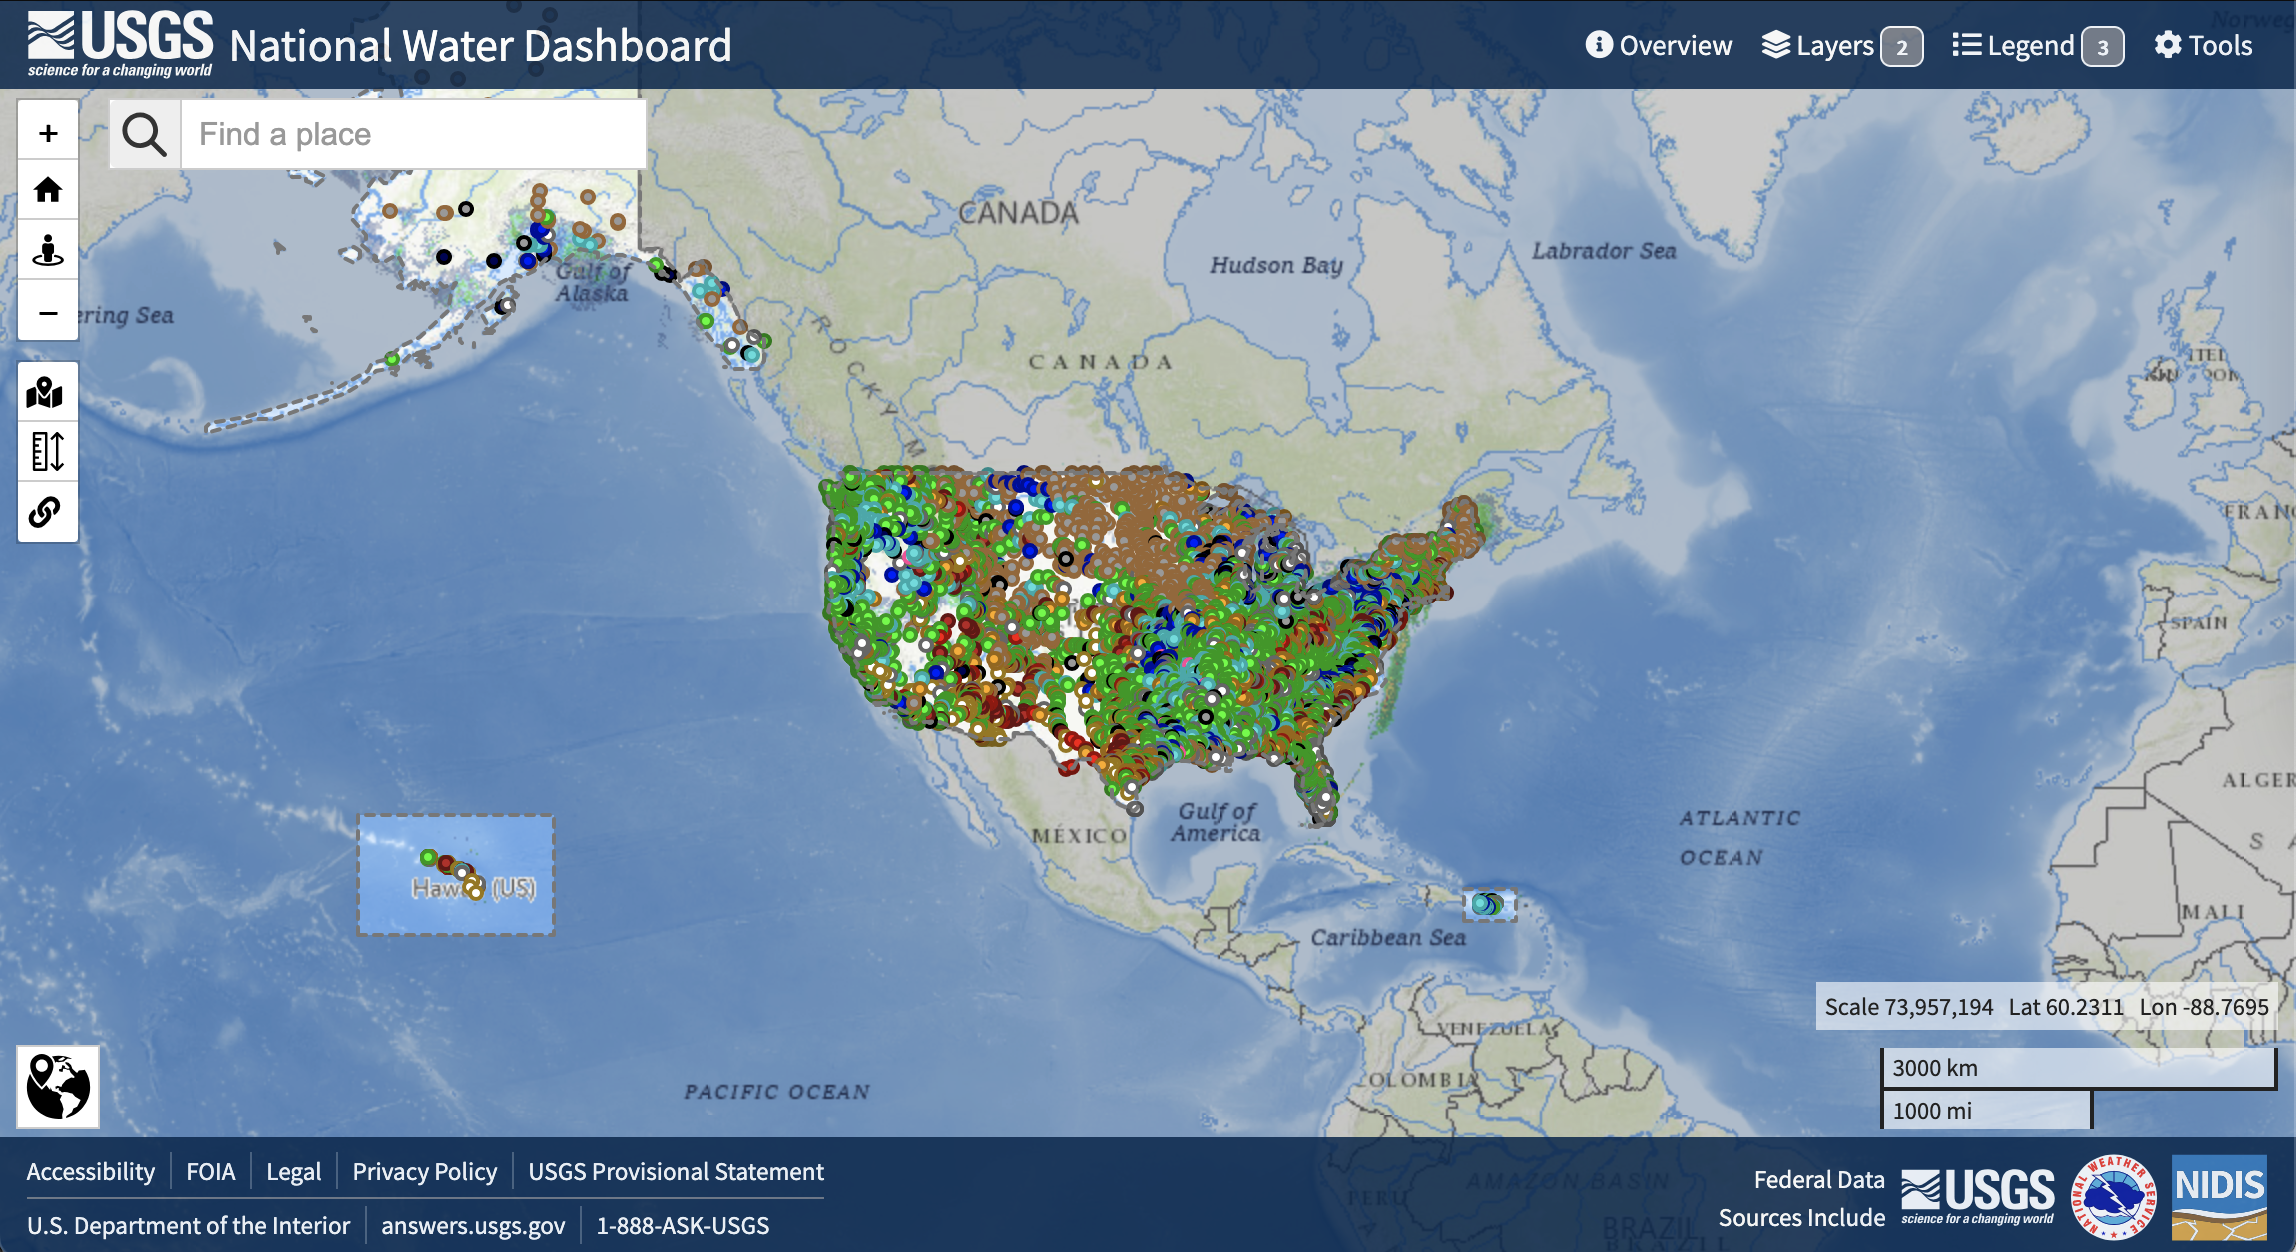
\includegraphics[keepaspectratio]{img/earth-analytics/flood-frequency/nwis-screenshots/01-nwis-dash.png}}

}

\caption{Go to the
\href{https://dashboard.waterdata.usgs.gov/app/nwd/en/}{National Water
Information System Mapper}}

\end{figure}%

\paragraph{Step 2: Search}\label{step-2-search}

\begin{figure}[H]

{\centering \pandocbounded{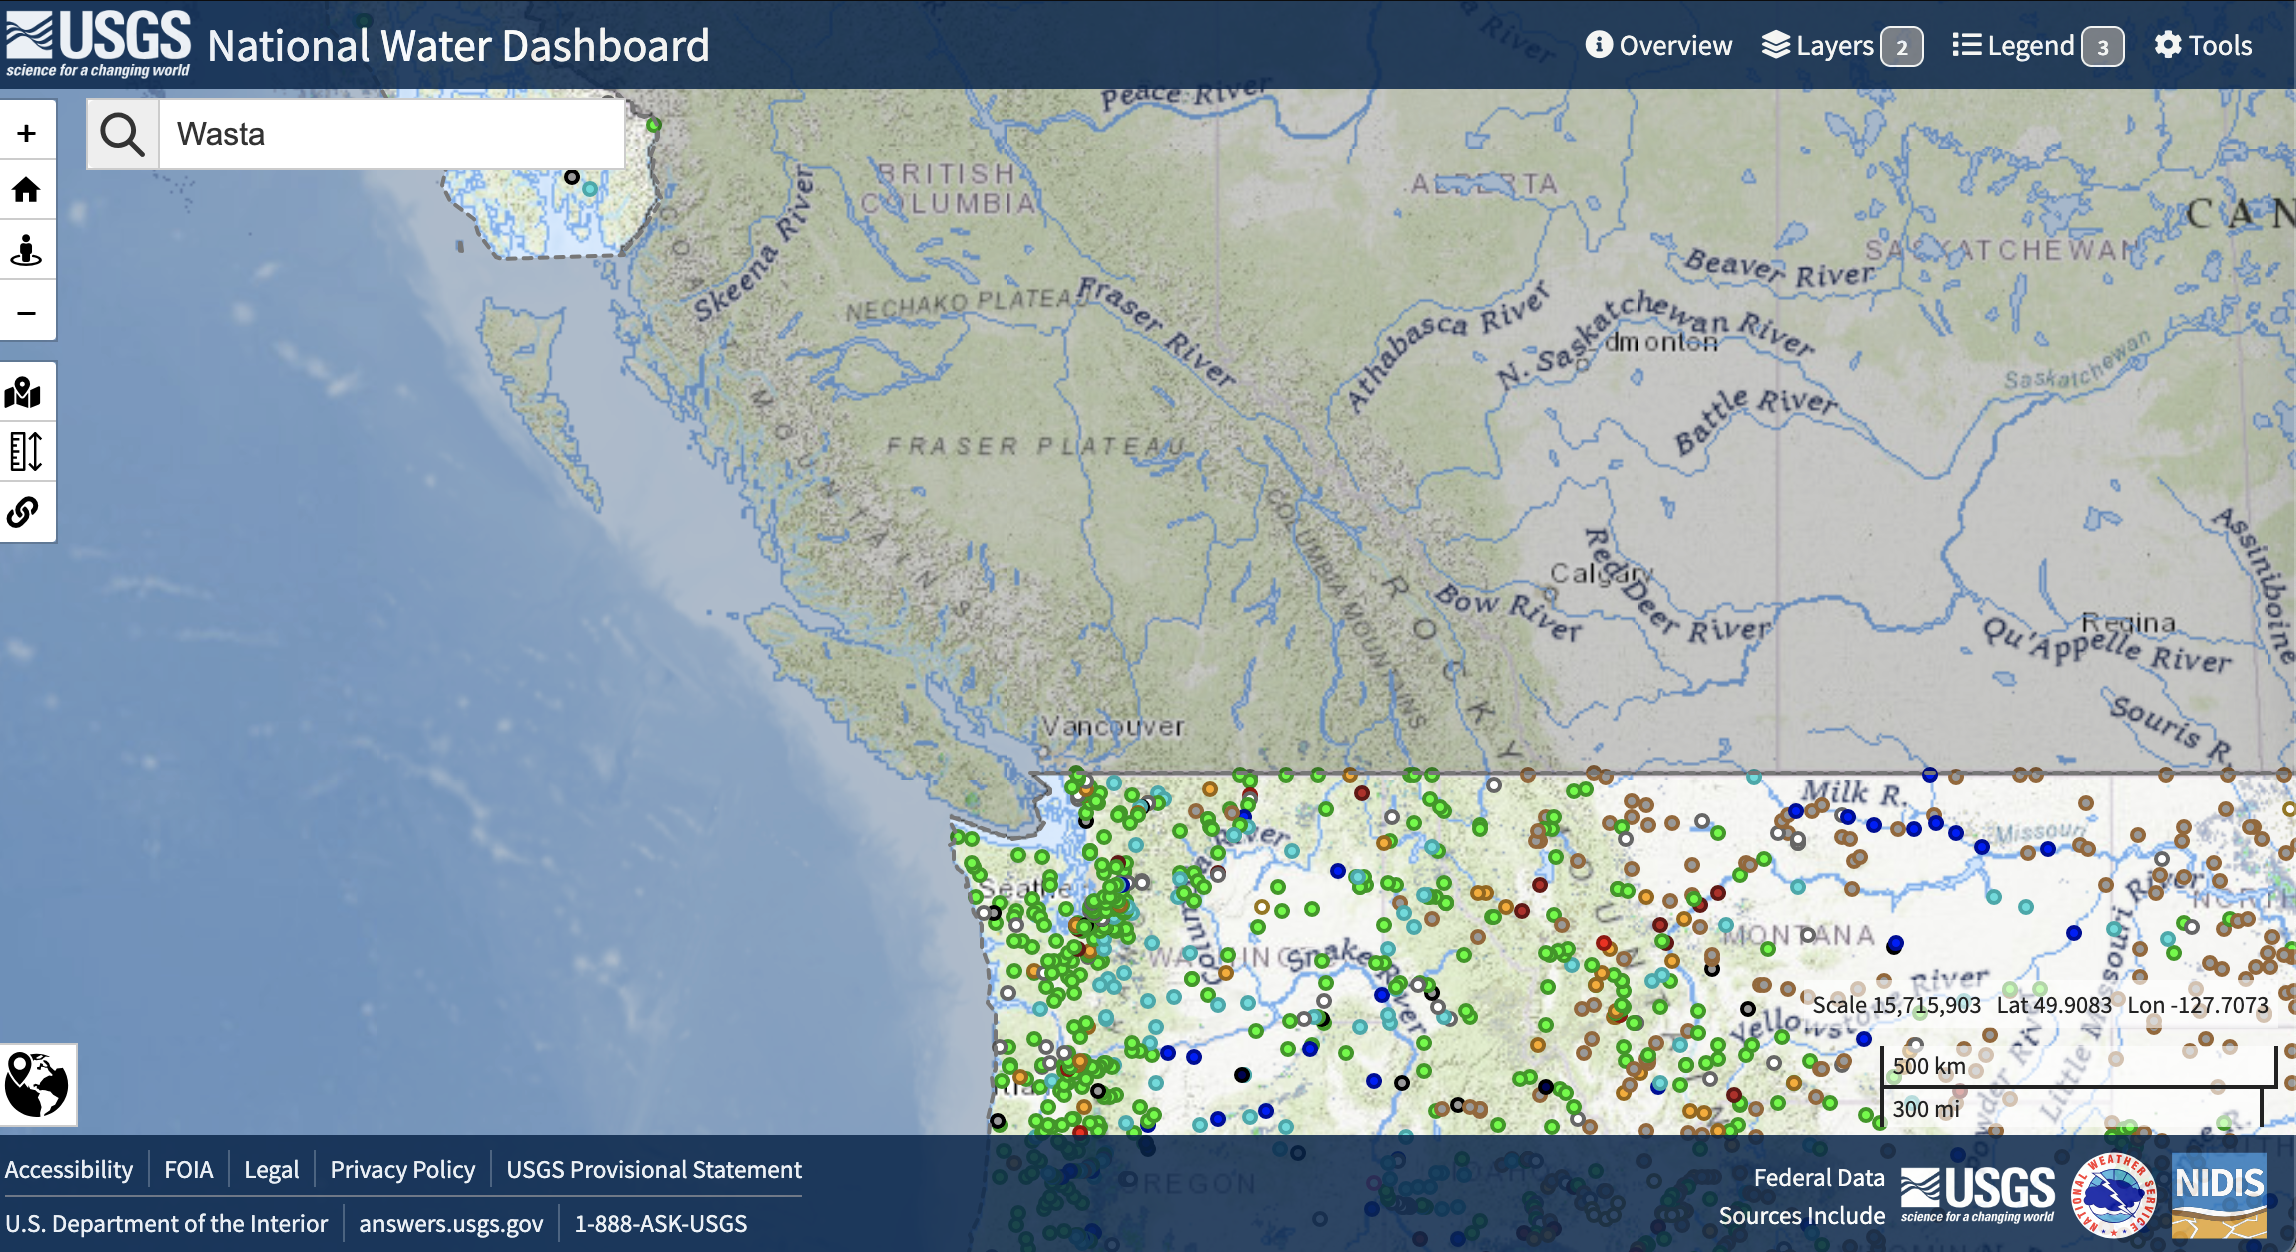
\includegraphics[keepaspectratio]{img/earth-analytics/flood-frequency/nwis-screenshots/02-place-search.png}}

}

\caption{Type in \texttt{Wasta} in the \texttt{Find\ a\ Place} box}

\end{figure}%

\paragraph{Step 3: Select gage}\label{step-3-select-gage}

\begin{figure}[H]

{\centering \pandocbounded{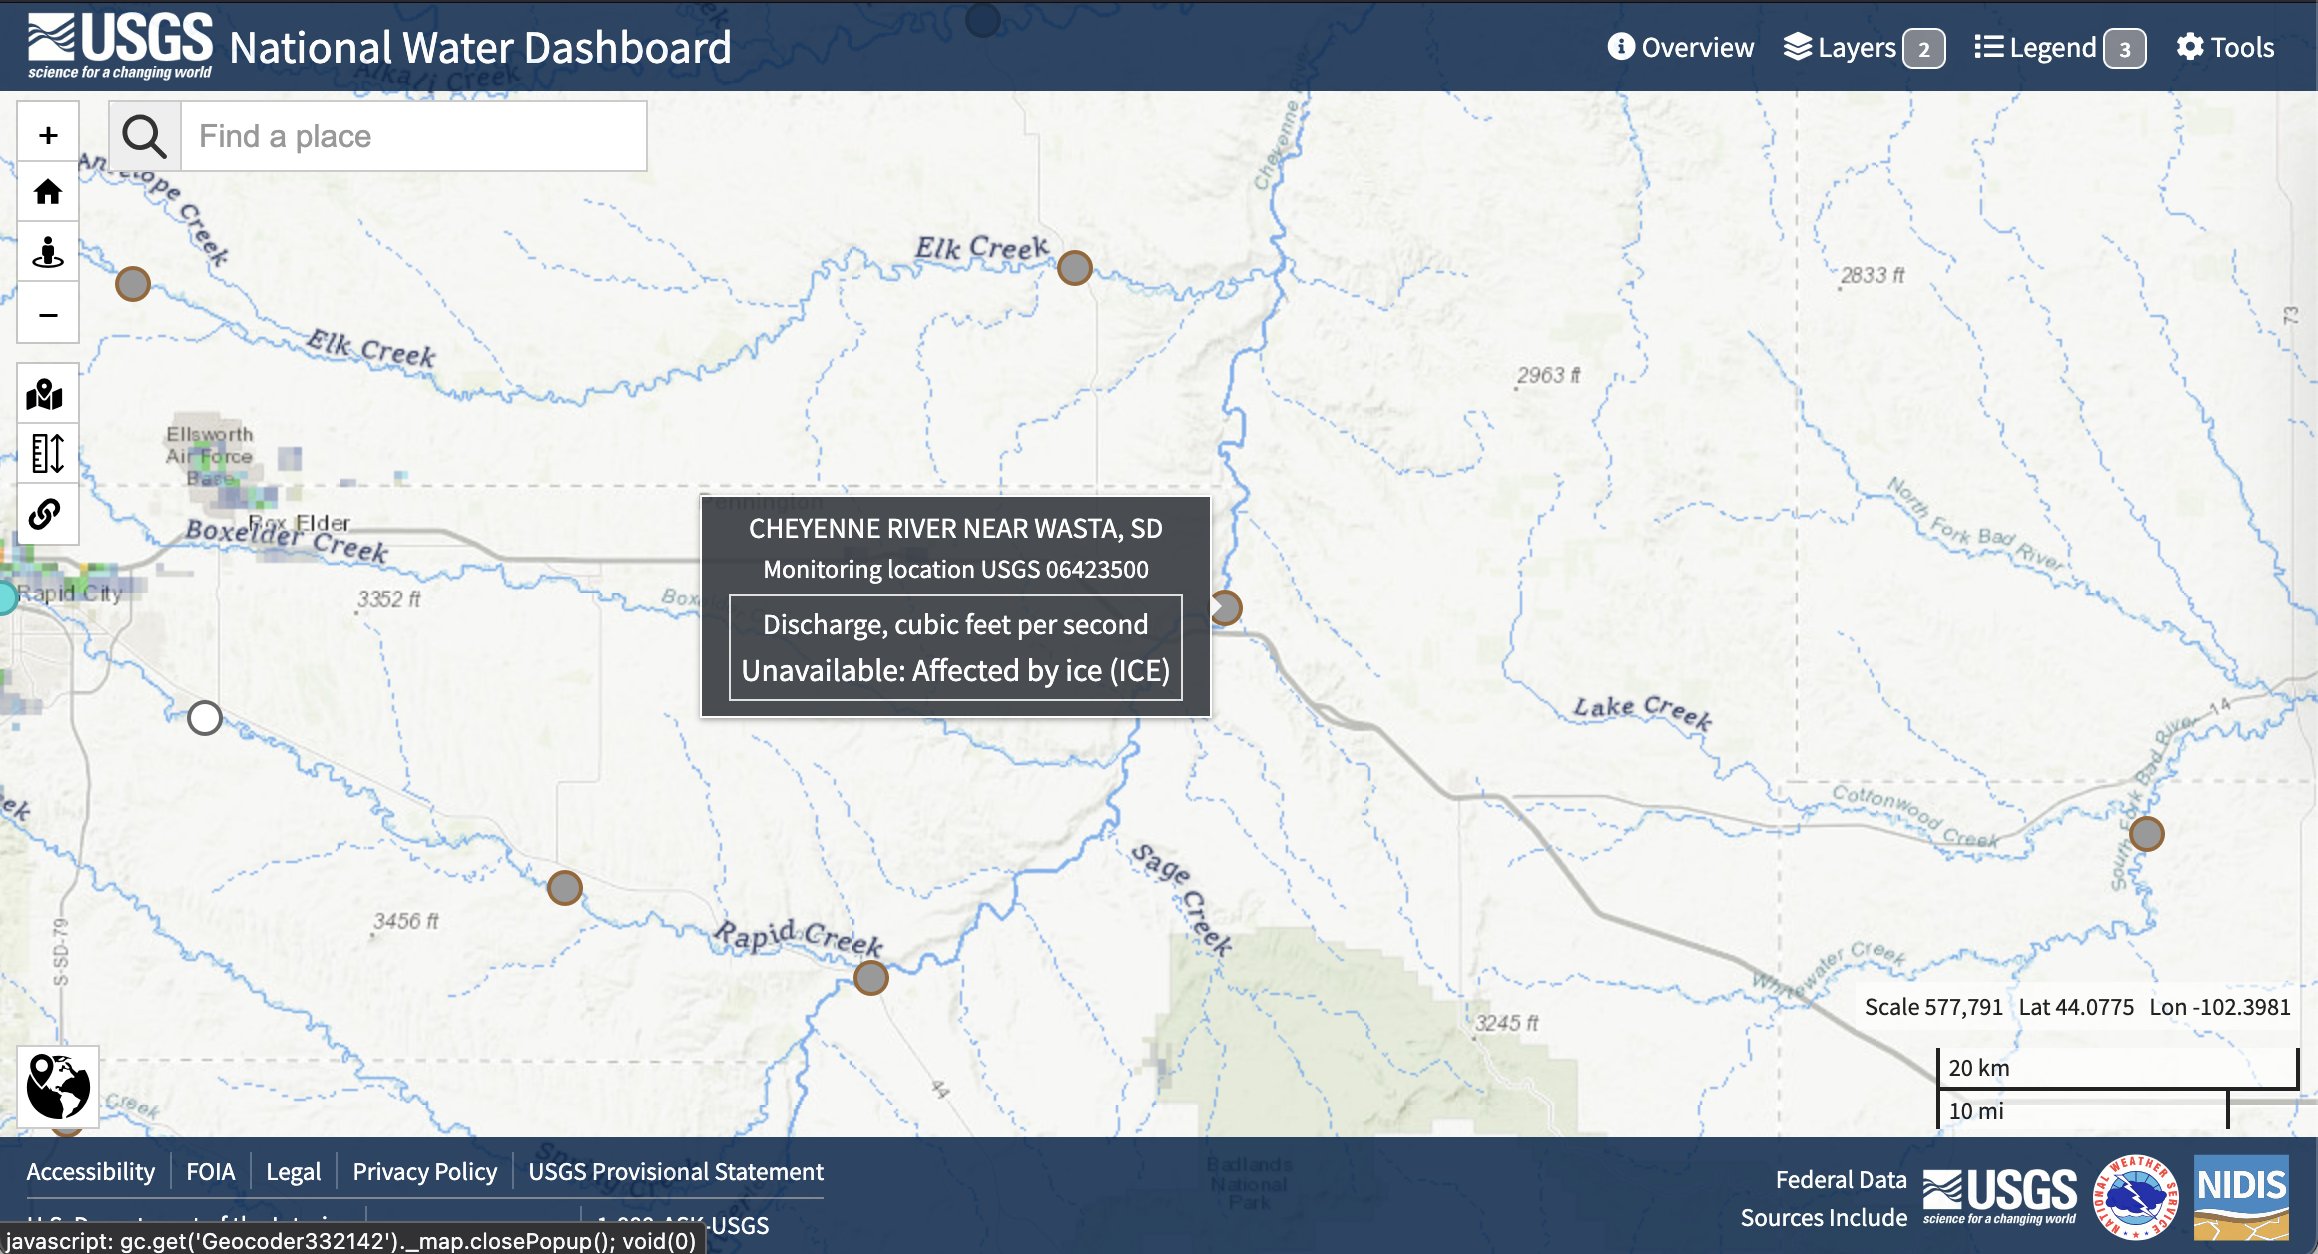
\includegraphics[keepaspectratio]{img/earth-analytics/flood-frequency/nwis-screenshots/03-open-gage.png}}

}

\caption{Click on the Cheyenne River near Wasta site. It should open a
new window.}

\end{figure}%

\paragraph{Step 4: Open site page}\label{step-4-open-site-page}

\begin{figure}[H]

{\centering \pandocbounded{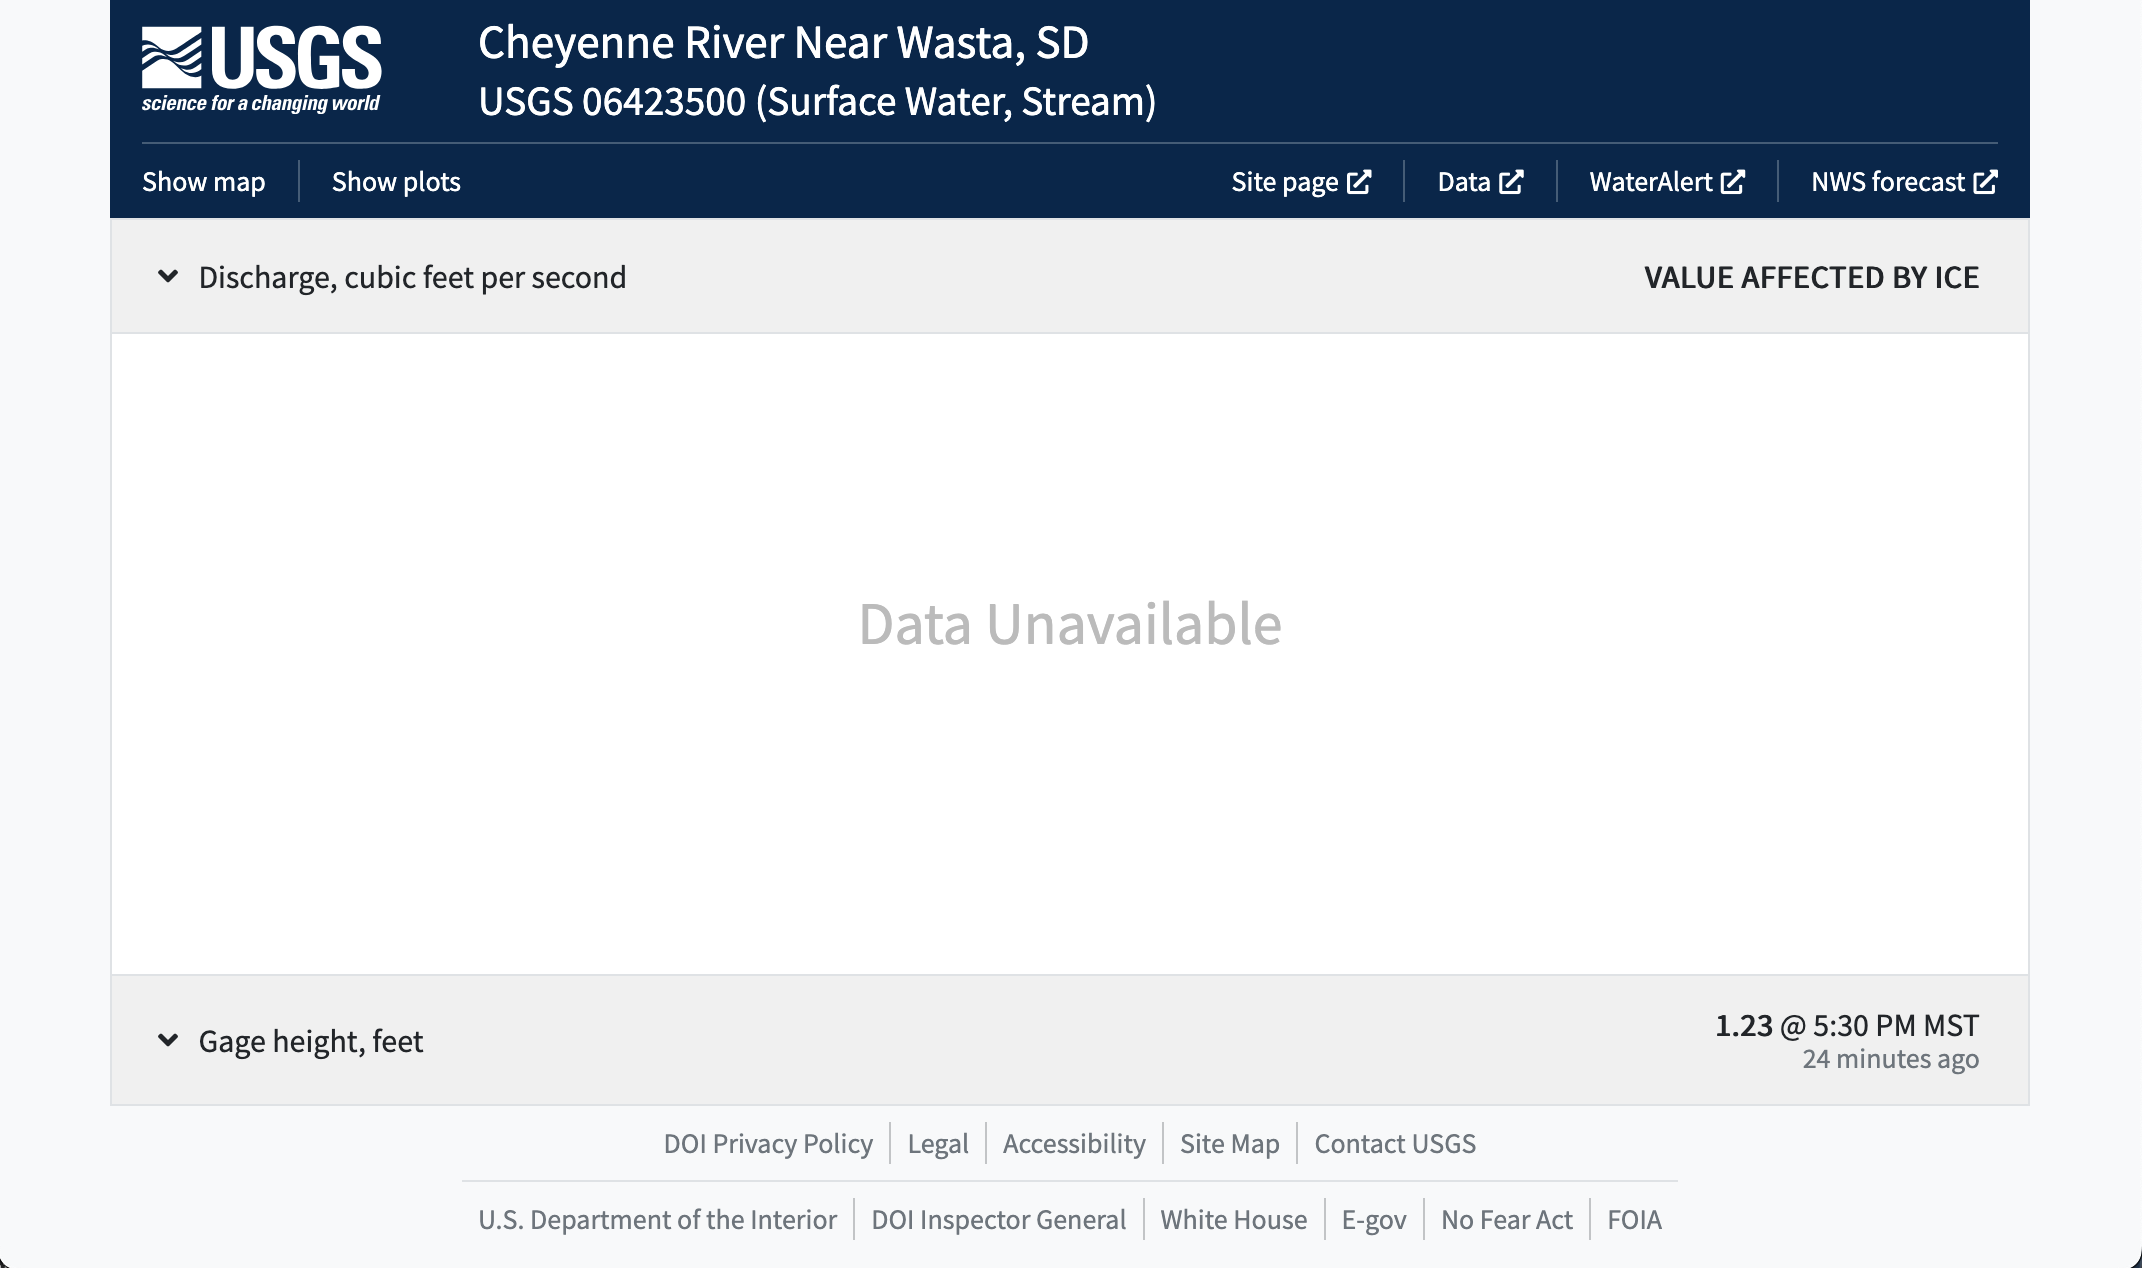
\includegraphics[keepaspectratio]{img/earth-analytics/flood-frequency/nwis-screenshots/04-open-site-info.png}}

}

\caption{Click on \texttt{Site\ page} at the top}

\end{figure}%

\begin{figure}[H]

{\centering \pandocbounded{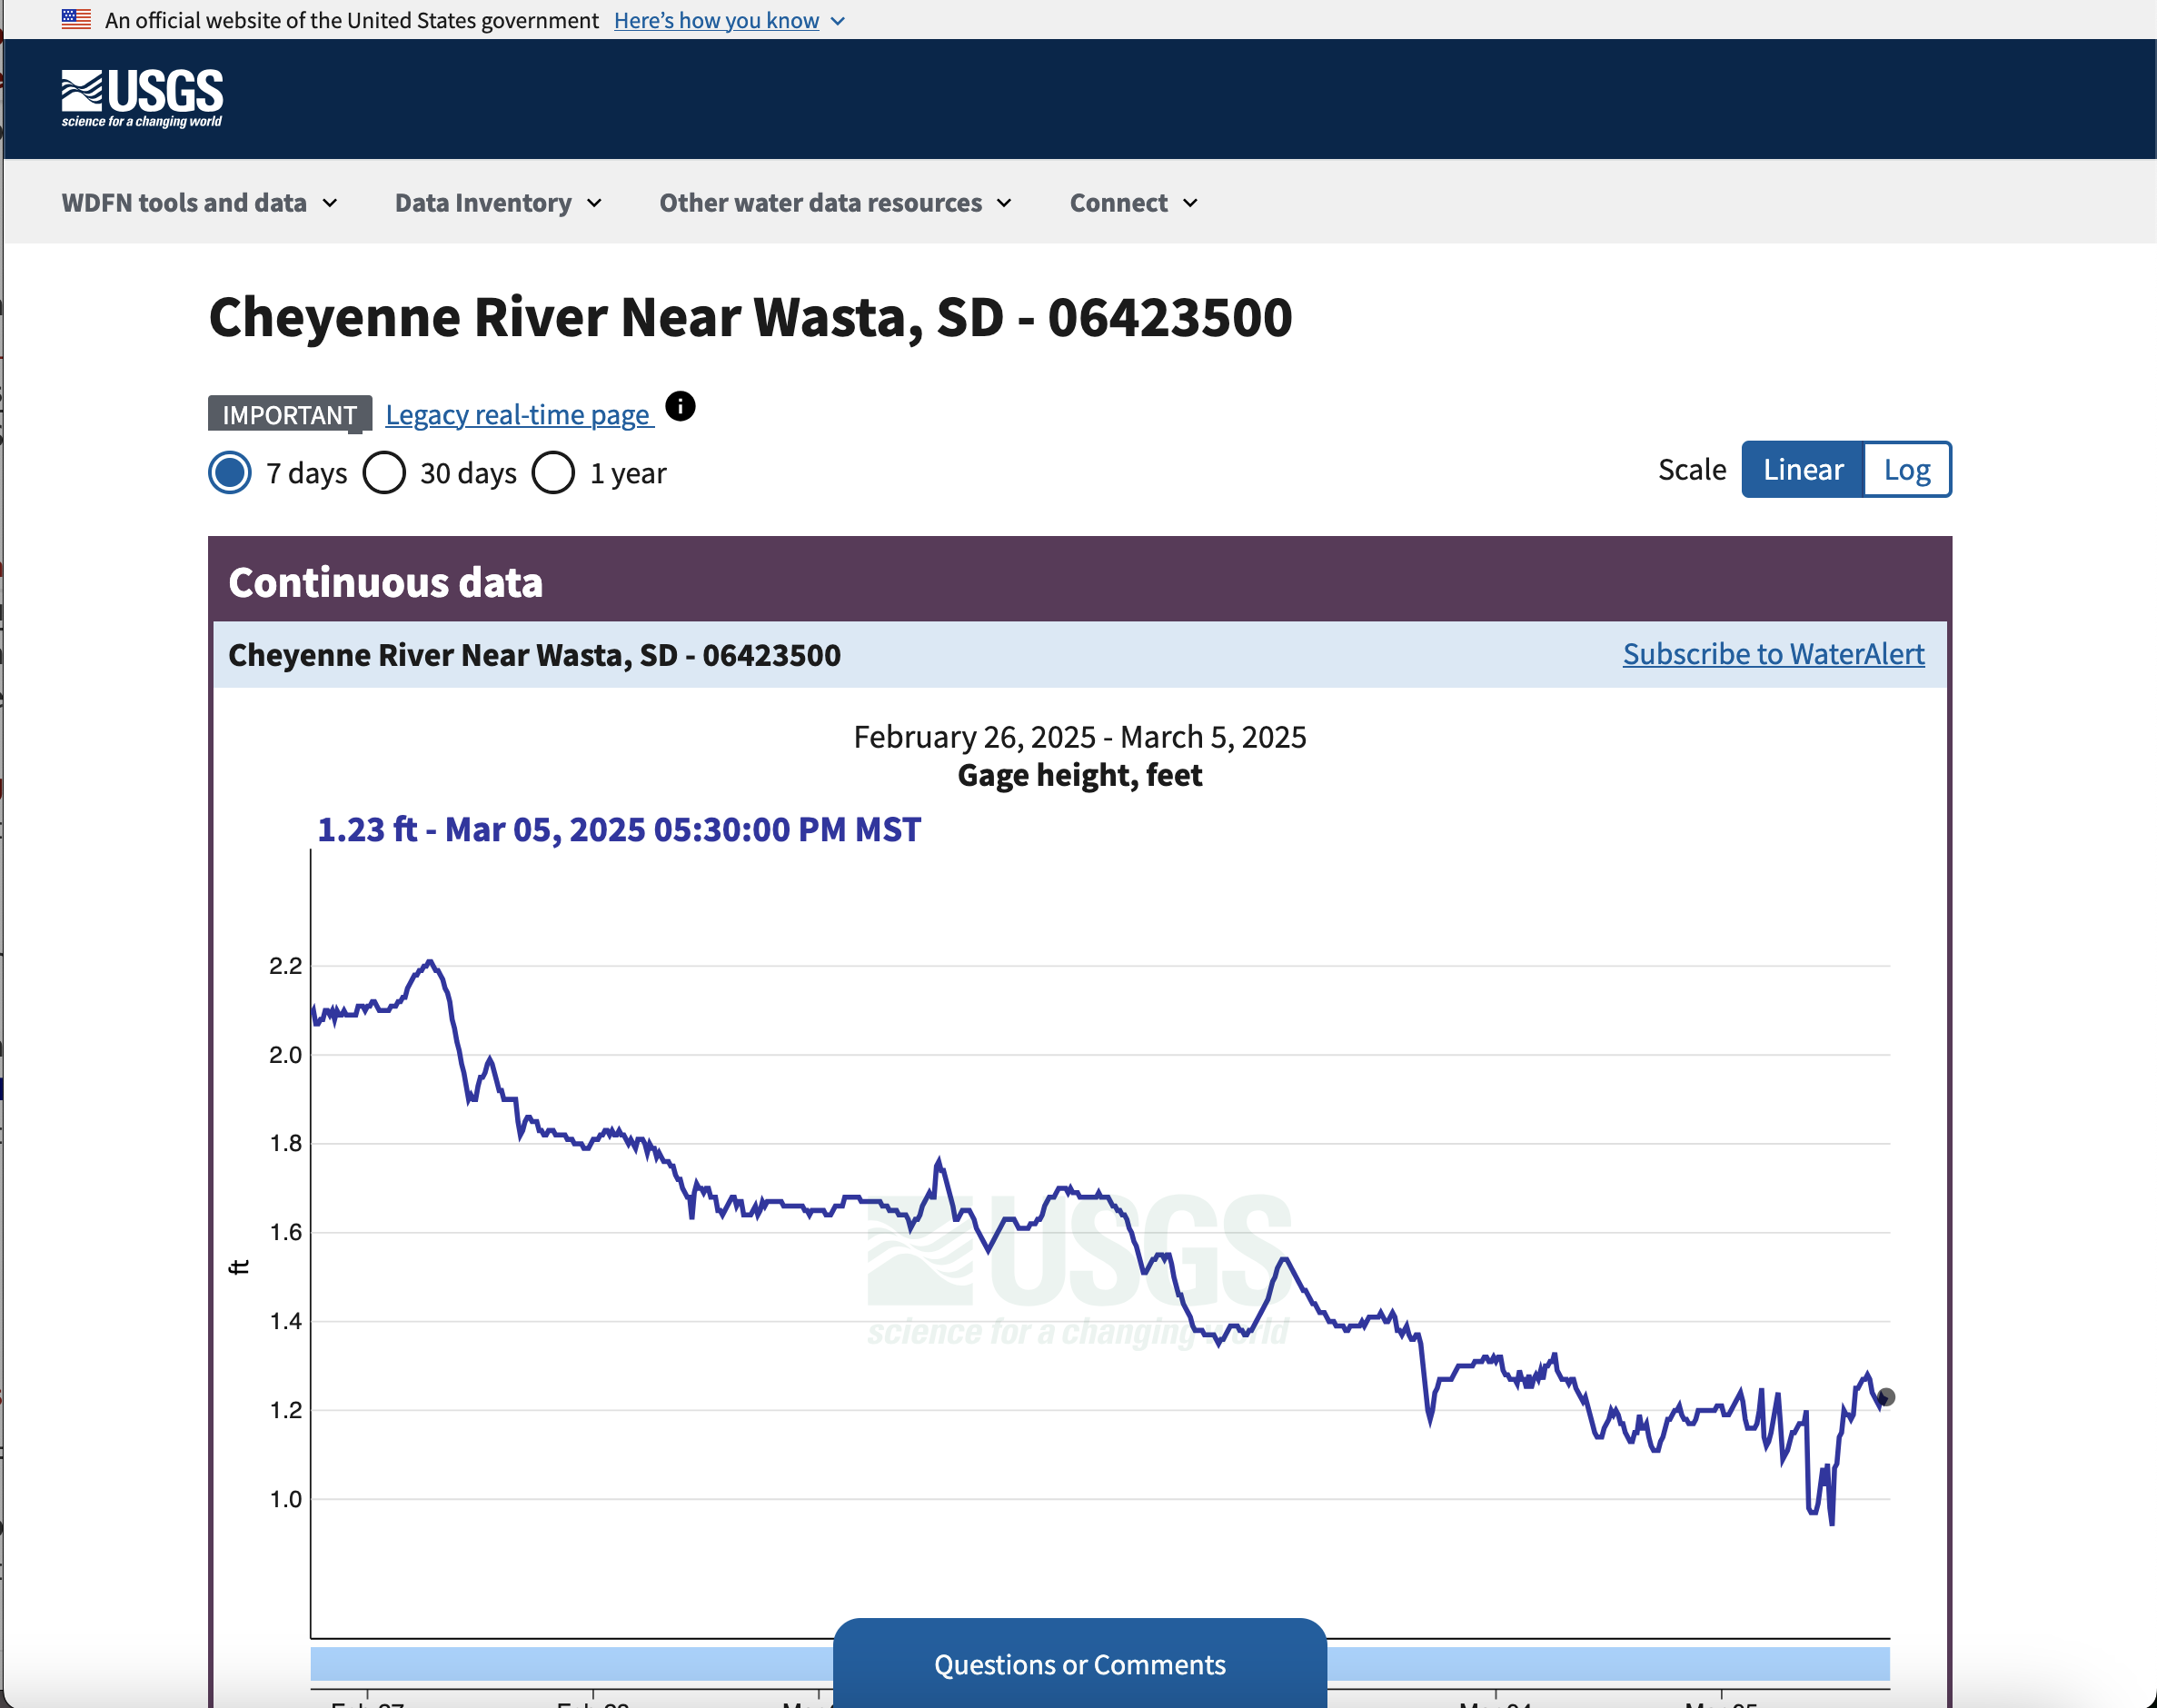
\includegraphics[keepaspectratio]{img/earth-analytics/flood-frequency/nwis-screenshots/05-site-info.png}}

}

\caption{You should now be on the Cheyenne River near Wasta gage site
page}

\end{figure}%

\paragraph{Step 5: Get coordinates}\label{step-5-get-coordinates}

\begin{figure}[H]

{\centering \pandocbounded{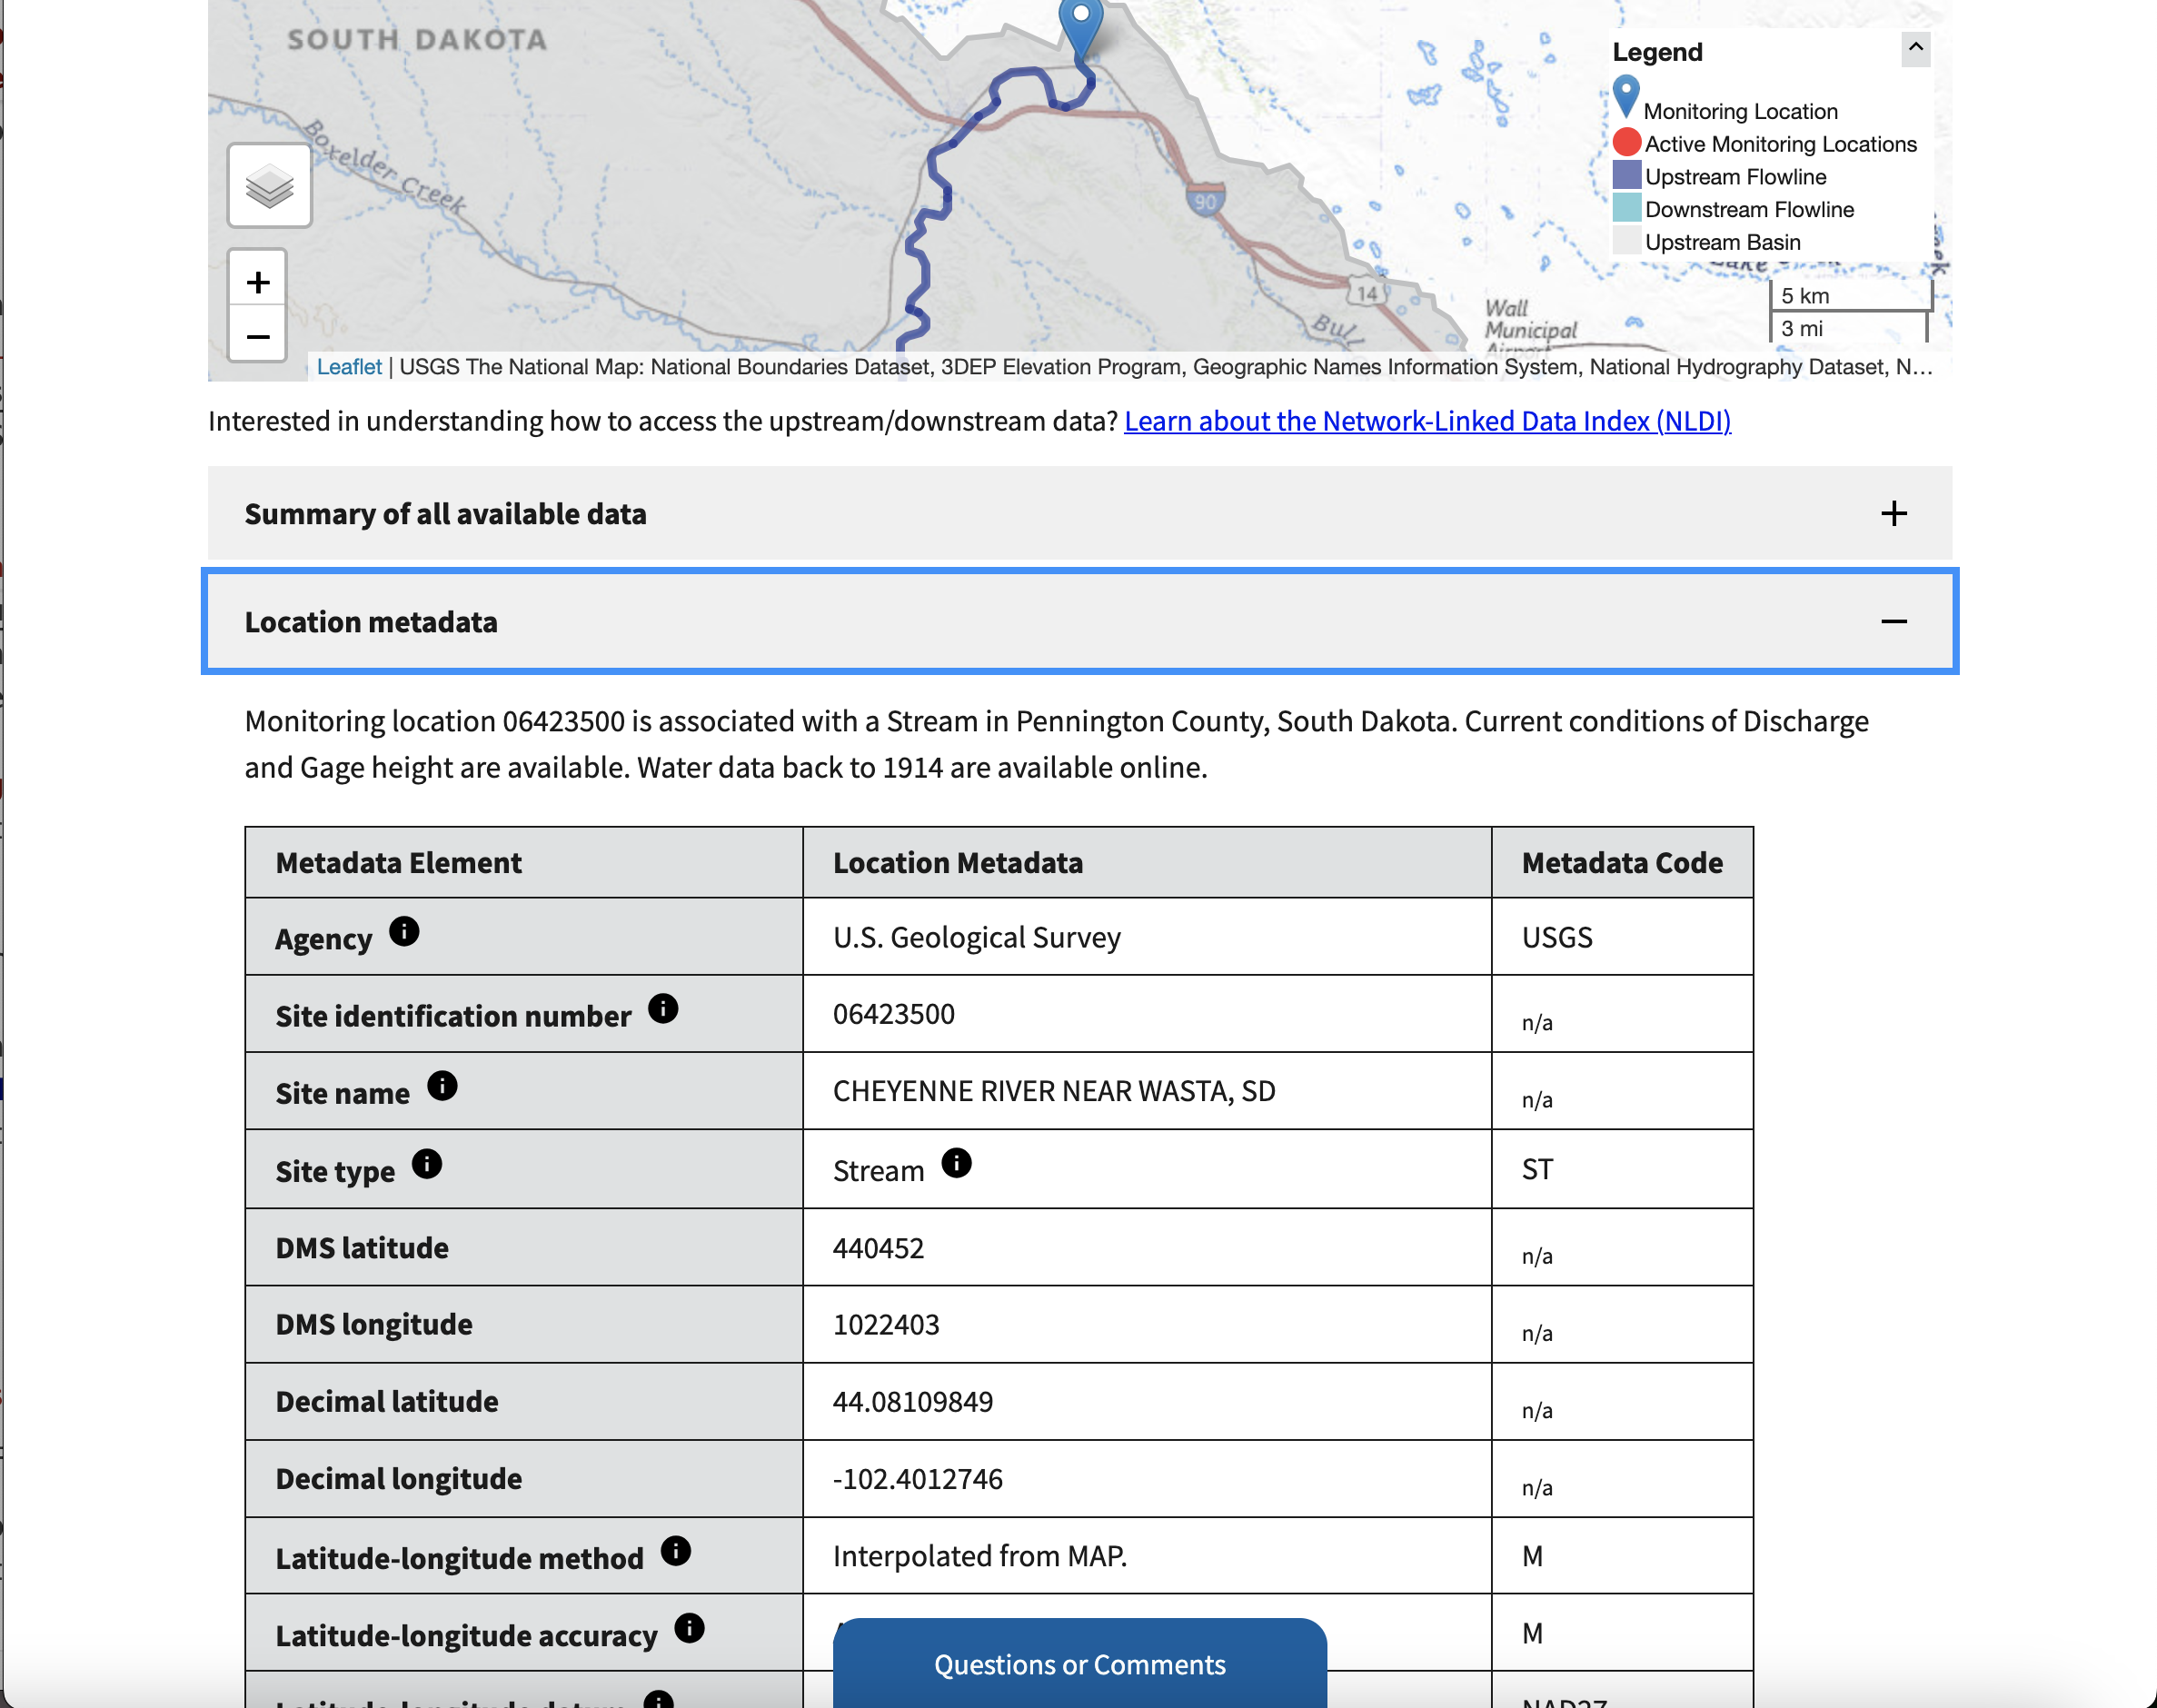
\includegraphics[keepaspectratio]{img/earth-analytics/flood-frequency/nwis-screenshots/06-get-latlon.png}}

}

\caption{Scroll to the bottom and open the \texttt{Location\ metadata}
section. Make a note of the decimal latitude and longitude!}

\end{figure}%

\begin{tcolorbox}[enhanced jigsaw, colbacktitle=quarto-callout-color!10!white, opacityback=0, bottomtitle=1mm, toptitle=1mm, bottomrule=.15mm, left=2mm, colframe=quarto-callout-color-frame, leftrule=.75mm, opacitybacktitle=0.6, colback=white, rightrule=.15mm, toprule=.15mm, breakable, titlerule=0mm, title=\textcolor{quarto-callout-color}{\faInfo}\hspace{0.5em}{Try It}, coltitle=black, arc=.35mm]

Now, you're ready to create your site map!

\begin{enumerate}
\def\labelenumi{\arabic{enumi}.}
\tightlist
\item
  Define latitude and longitude variables to \textbf{match the variable
  names used in the code}.
\item
  Rename the variable \texttt{gdf} with something \textbf{descriptive}
  wherever it occurs.
\item
  Run and test your cell to make sure everything works.
\end{enumerate}

\end{tcolorbox}

\begin{tcolorbox}[enhanced jigsaw, colbacktitle=quarto-callout-color!10!white, opacityback=0, bottomtitle=1mm, toptitle=1mm, bottomrule=.15mm, left=2mm, colframe=quarto-callout-color-frame, leftrule=.75mm, opacitybacktitle=0.6, colback=white, rightrule=.15mm, toprule=.15mm, breakable, titlerule=0mm, title=\textcolor{quarto-callout-color}{\faInfo}\hspace{0.5em}{Looking for an Extra Challenge?}, coltitle=black, arc=.35mm]

Customize your plot \href{https://hvplot.holoviz.org/index.html}{using
the hvplot documentation} or by asking your favorite AI tool. For
example, you could:

\begin{itemize}
\tightlist
\item
  Change the size of your map
\item
  Change the base map images
\item
  Change the color and size of your place marker
\item
  Remove the axis labels for a cleaner map
\end{itemize}

\end{tcolorbox}

\begin{Shaded}
\begin{Highlighting}[]
\CommentTok{\# Create a GeoDataFrame with the gage location}
\NormalTok{gdf }\OperatorTok{=}\NormalTok{ gpd.GeoDataFrame(}
    \CommentTok{\# Create the geometry from lat/lon}
\NormalTok{    geometry}\OperatorTok{=}\NormalTok{gpd.points\_from\_xy([gage\_lon], [gage\_lat]),}
    \CommentTok{\# Coordinate Reference System for lat/lon values}
\NormalTok{    crs}\OperatorTok{=}\StringTok{"EPSG:4326"}
\NormalTok{)}

\CommentTok{\# Plot using hvPlot with a basemap}
\BuiltInTok{buffer} \OperatorTok{=} \FloatTok{0.01}
\NormalTok{gdf.hvplot.points(}
    \CommentTok{\# Use web tile basemap imagery}
\NormalTok{    geo}\OperatorTok{=}\VariableTok{True}\NormalTok{, tiles}\OperatorTok{=}\StringTok{\textquotesingle{}OpenTopoMap\textquotesingle{}}\NormalTok{, }
    \CommentTok{\# Set approximate bounding box}
\NormalTok{    ylim}\OperatorTok{=}\NormalTok{(gage\_lat}\OperatorTok{{-}}\BuiltInTok{buffer}\NormalTok{, gage\_lat}\OperatorTok{+}\BuiltInTok{buffer}\NormalTok{),}
\NormalTok{    xlim}\OperatorTok{=}\NormalTok{(gage\_lon}\OperatorTok{{-}}\BuiltInTok{buffer}\NormalTok{, gage\_lon}\OperatorTok{+}\BuiltInTok{buffer}\NormalTok{),}
\NormalTok{)}
\end{Highlighting}
\end{Shaded}

\section{STEP 2 Data wrangling}\label{step-2-data-wrangling}

\subsection{Load sample data}\label{load-sample-data}

You should now have the sample data downloaded, but you still need to
open it up so you can use it. First, you'll need the path to your data.

\begin{tcolorbox}[enhanced jigsaw, colbacktitle=quarto-callout-color!10!white, opacityback=0, bottomtitle=1mm, toptitle=1mm, bottomrule=.15mm, left=2mm, colframe=quarto-callout-color-frame, leftrule=.75mm, opacitybacktitle=0.6, colback=white, rightrule=.15mm, toprule=.15mm, breakable, titlerule=0mm, title=\textcolor{quarto-callout-color}{\faInfo}\hspace{0.5em}{Try It}, coltitle=black, arc=.35mm]

\begin{enumerate}
\def\labelenumi{\arabic{enumi}.}
\tightlist
\item
  Replace \texttt{data\_path} with a descriptive name
\item
  Check your data directory for the file name of the streamflow data,
  and put it in the place of \texttt{data-filename-here}
\end{enumerate}

\end{tcolorbox}

\begin{Shaded}
\begin{Highlighting}[]
\NormalTok{data\_path }\OperatorTok{=}\NormalTok{ project.project\_dir }\OperatorTok{/} \StringTok{\textquotesingle{}data{-}filename{-}here.csv\textquotesingle{}}
\end{Highlighting}
\end{Shaded}

Let's take a look at the raw data (make sure to replace
\texttt{nwis\_path} with the name of your variable!):

\begin{Shaded}
\begin{Highlighting}[]
\OperatorTok{!}\NormalTok{head }\OperatorTok{{-}}\NormalTok{n }\DecValTok{5}\NormalTok{ $nwis\_path}
\end{Highlighting}
\end{Shaded}

\begin{verbatim}
head: /Users/elsa/Library/Application: No such file or directory
head: Support/earth-analytics/flood-cheyenne/cheyenne_streamflow_1934_2024.csv: No such file or directory
\end{verbatim}

\begin{tcolorbox}[enhanced jigsaw, colbacktitle=quarto-callout-color!10!white, opacityback=0, bottomtitle=1mm, toptitle=1mm, bottomrule=.15mm, left=2mm, colframe=quarto-callout-color-frame, leftrule=.75mm, opacitybacktitle=0.6, colback=white, rightrule=.15mm, toprule=.15mm, breakable, titlerule=0mm, title=\textcolor{quarto-callout-color}{\faInfo}\hspace{0.5em}{Try It}, coltitle=black, arc=.35mm]

The cell below imports \texttt{CSV} data like the flood data into
Python. A useful method for looking at the \textbf{datatypes} in your
\texttt{pd.DataFrame} is the \texttt{pd.DataFrame.info()} method.

\begin{enumerate}
\def\labelenumi{\arabic{enumi}.}
\tightlist
\item
  Replace \texttt{dataframe} with a descriptive name for your DataFrame
  variable
\item
  Run the cell to see the datatypes of each column.
\item
  Try \textbf{uncommenting} lines one by one by deleting the \texttt{\#}
  at the beginning and running the code again.
\end{enumerate}

What changes? Why do you think those lines are needed?

\end{tcolorbox}

\begin{tcolorbox}[enhanced jigsaw, colbacktitle=quarto-callout-tip-color!10!white, opacityback=0, bottomtitle=1mm, toptitle=1mm, bottomrule=.15mm, left=2mm, colframe=quarto-callout-tip-color-frame, leftrule=.75mm, opacitybacktitle=0.6, colback=white, rightrule=.15mm, toprule=.15mm, breakable, titlerule=0mm, title=\textcolor{quarto-callout-tip-color}{\faLightbulb}\hspace{0.5em}{Tip}, coltitle=black, arc=.35mm]

In Python, you will see both \textbf{methods} and \textbf{functions}
when you want to give the computer some instructions. This is an
\emph{important and tricky} distinction. For right now -- functions have
all of their arguments/parameters \textbf{inside} the parentheses, as in
\texttt{dataretrieval.nwis.get\_discharge\_measurements()}. For
\textbf{methods}, the first argument is always some kind of Python
object that is placed \textbf{before} the method. For example, take a
look at the next cell for an example of using the
\texttt{pd.DataFrame.info()} \textbf{method}.

\end{tcolorbox}

\begin{Shaded}
\begin{Highlighting}[]
\NormalTok{dataframe }\OperatorTok{=}\NormalTok{ pd.read\_csv(}
\NormalTok{    data\_path,}
    \CommentTok{\#index\_col=\textquotesingle{}datetime\textquotesingle{},}
    \CommentTok{\#parse\_dates=True)}
\NormalTok{dataframe.info()}
\end{Highlighting}
\end{Shaded}

\begin{tcolorbox}[enhanced jigsaw, colbacktitle=quarto-callout-color!10!white, opacityback=0, bottomtitle=1mm, toptitle=1mm, bottomrule=.15mm, left=2mm, colframe=quarto-callout-color-frame, leftrule=.75mm, opacitybacktitle=0.6, colback=white, rightrule=.15mm, toprule=.15mm, breakable, titlerule=0mm, title=\textcolor{quarto-callout-color}{\faInfo}\hspace{0.5em}{Reflect and Respond}, coltitle=black, arc=.35mm]

What column do you think the streamflow, or discharge, measurements are
in?

\end{tcolorbox}

\subsection{Organize your data
descriptively}\label{organize-your-data-descriptively}

It's important to make sure that your code is easy to read. Even if you
don't plan to share it, \textbf{you} will likely need to read code
you've written in the future!

\begin{tcolorbox}[enhanced jigsaw, colbacktitle=quarto-callout-color!10!white, opacityback=0, bottomtitle=1mm, toptitle=1mm, bottomrule=.15mm, left=2mm, colframe=quarto-callout-color-frame, leftrule=.75mm, opacitybacktitle=0.6, colback=white, rightrule=.15mm, toprule=.15mm, breakable, titlerule=0mm, title=\textcolor{quarto-callout-color}{\faInfo}\hspace{0.5em}{Try It}, coltitle=black, arc=.35mm]

Using the code below as a starting point, select the discharge column
and rename it to something descriptive:

\begin{enumerate}
\def\labelenumi{\arabic{enumi}.}
\tightlist
\item
  Identify the discharge/streamflow column.
\item
  Replace \texttt{discharge\_column\_name} with the discharge column
  name.
\item
  Replace \texttt{new\_column\_name} with a descriptive name. We
  recommend including the \textbf{units} of the discharge values in the
  column name as a way to keep track of them.
\end{enumerate}

\end{tcolorbox}

\begin{Shaded}
\begin{Highlighting}[]
\NormalTok{discharge\_df }\OperatorTok{=}\NormalTok{ (}
\NormalTok{    nwis\_df}
    \CommentTok{\# Select only the discharge column as a DataFrame}
\NormalTok{    [[}\StringTok{\textquotesingle{}discharge\_column\_name\textquotesingle{}}\NormalTok{]]}
    \CommentTok{\# Rename the discharge column}
\NormalTok{    .rename(columns}\OperatorTok{=}\NormalTok{\{}\StringTok{\textquotesingle{}discharge\_column\_name\textquotesingle{}}\NormalTok{: }\StringTok{\textquotesingle{}new\_column\_name\textquotesingle{}}\NormalTok{\})}
\NormalTok{)}

\NormalTok{discharge\_df}
\end{Highlighting}
\end{Shaded}

\begin{tcolorbox}[enhanced jigsaw, colbacktitle=quarto-callout-tip-color!10!white, opacityback=0, bottomtitle=1mm, toptitle=1mm, bottomrule=.15mm, left=2mm, colframe=quarto-callout-tip-color-frame, leftrule=.75mm, opacitybacktitle=0.6, colback=white, rightrule=.15mm, toprule=.15mm, breakable, titlerule=0mm, title=\textcolor{quarto-callout-tip-color}{\faLightbulb}\hspace{0.5em}{Strings}, coltitle=black, arc=.35mm]

How does a computer tell the difference between a \textbf{name} which is
linked to a value, and a \textbf{string} of characters to be interpreted
as text (like a column name)?

In most programming languages, we have to put quotes around strings of
characters that are meant to be interpreted \textbf{literally} as text
rather than \textbf{symbolically} as a variable. In Python, you can use
either single \texttt{\textquotesingle{}} or double \texttt{"} quotes
around strings. If you forget to put quotes around your strings, Python
will try to interpret them as variable \textbf{names} instead, and will
probably give you a \texttt{NameError} when it can't find the linked
value.

\end{tcolorbox}

\section{STEP 3: Visualize the flood}\label{step-3-visualize-the-flood}

Visualizing the data will help make sure that everything is formatted
correctly and makes sense. It also helps later on with communicating
your results.

\subsection{Can we see the flood in the streamflow
data?}\label{can-we-see-the-flood-in-the-streamflow-data}

Let's take a look at the data from February - September, 2019. This
should let us see the peak streamflow values and when they occurred.

\begin{tcolorbox}[enhanced jigsaw, colbacktitle=quarto-callout-color!10!white, opacityback=0, bottomtitle=1mm, toptitle=1mm, bottomrule=.15mm, left=2mm, colframe=quarto-callout-color-frame, leftrule=.75mm, opacitybacktitle=0.6, colback=white, rightrule=.15mm, toprule=.15mm, breakable, titlerule=0mm, title=\textcolor{quarto-callout-color}{\faInfo}\hspace{0.5em}{Try It}, coltitle=black, arc=.35mm]

Below, you will see an example of how to subset your streamflow data by
date.We do this using the \texttt{.loc} attribute of your
\texttt{DataFrame}, which is a powerful tool for selecting the rows you
want. Because the dates are in the Python \texttt{datetime64} format,
you can select based on the year and month, without needing to type out
dates or times!

\begin{enumerate}
\def\labelenumi{\arabic{enumi}.}
\tightlist
\item
  Replace \texttt{dataframe\_name} with your streamflow
  \texttt{DataFrame} name.
\item
  Save the result to a descriptive variable name, and call it at the end
  of the cell for testing.
\end{enumerate}

\end{tcolorbox}

You can find some
\href{https://www.earthdatascience.org/courses/use-data-open-source-python/use-time-series-data-in-python/date-time-types-in-pandas-python/subset-time-series-data-python/}{examples
of subsetting time series data in the textbook}.

\begin{Shaded}
\begin{Highlighting}[]
\NormalTok{dataframe\_name.loc[}\StringTok{\textquotesingle{}2019{-}02\textquotesingle{}}\NormalTok{:}\StringTok{\textquotesingle{}2019{-}09\textquotesingle{}}\NormalTok{]}
\end{Highlighting}
\end{Shaded}

\subsection{Create a line plot with
Python}\label{create-a-line-plot-with-python}

Next, plot your subsetted data. Don't forget to label your plot!

\begin{tcolorbox}[enhanced jigsaw, colbacktitle=quarto-callout-color!10!white, opacityback=0, bottomtitle=1mm, toptitle=1mm, bottomrule=.15mm, left=2mm, colframe=quarto-callout-color-frame, leftrule=.75mm, opacitybacktitle=0.6, colback=white, rightrule=.15mm, toprule=.15mm, breakable, titlerule=0mm, title=\textcolor{quarto-callout-color}{\faInfo}\hspace{0.5em}{Try It}, coltitle=black, arc=.35mm]

\end{tcolorbox}

\begin{Shaded}
\begin{Highlighting}[]
\NormalTok{(}
\NormalTok{    dataframe\_name}
\NormalTok{    .plot(}
\NormalTok{        xlabel}\OperatorTok{=}\StringTok{\textquotesingle{}\textquotesingle{}}\NormalTok{, }
\NormalTok{        ylabel}\OperatorTok{=}\StringTok{\textquotesingle{}\textquotesingle{}}\NormalTok{,}
\NormalTok{        title}\OperatorTok{=}\StringTok{\textquotesingle{}\textquotesingle{}}\NormalTok{)}
\NormalTok{)}
\end{Highlighting}
\end{Shaded}

You should be able to see the flood in your data going up above 12000
cfs at its peak! In the next section, you'll analyze how unusual that
is.

\section{STEP 4: Analyse the flood}\label{step-4-analyse-the-flood}

As scientists and engineers, we are interested in not just describing a
flood, but in understanding how often we would expect an event that
severe or extreme to happen. Some applications we need this information
for include:

\begin{itemize}
\tightlist
\item
  Designing and developing engineering standards for bridges and roads
  to withstand flooding
\item
  Choosing the capacity of water treatment plants to accommodate flood
  waters
\item
  Computing flood risk maps and choosing where to build
\item
  Determining flood insurance rates
\end{itemize}

The exceedance probability is a simple, data-driven way to quantify how
unusual a flood is and how often we can expect similar events to happen.
We calculate exceedance probability by counting how many years with
floods the same size or larger have been recorded, or ranking the and
dividing by the number of years we have records for:

\[P_e = \frac{\text{Annual peak flow rank}}{\text{Years of record}}\]

This value tells us historically what the likelihood was of a flood of a
certain size or larger each year, or the \textbf{exceedance
probability}. We can also express how unusual a flood is with the
\textbf{return period}, or an amount of time during which we'd expect
there to be about one flood the same size or larger. The return period
is the reciprocal of the exceedance probability:

\[R = \frac{\text{Years of record}}{\text{Annual peak flow rank}}\]

As an example -- suppose a streamflow of \(10000\) cfs occurs \(4\)
times over a 100-year record. The exceedance probability would be
\(\frac{4}{100} = .25\) and the return period would be 25 years.

There are advantages and disadvantages to this method of calculating the
\textbf{exceedance probability}. On one hand, we are not making any
assumptions about how often floods occur, and there is no way to
extrapolate to a size of flood that has never been observed. On the
other hand, we can't incorporate any information about how often floods
occur nearby or in other locations, and the data record for streamflow
is often less than the desired lifetime of the built environment.

\begin{tcolorbox}[enhanced jigsaw, colbacktitle=quarto-callout-color!10!white, opacityback=0, bottomtitle=1mm, toptitle=1mm, bottomrule=.15mm, left=2mm, colframe=quarto-callout-color-frame, leftrule=.75mm, opacitybacktitle=0.6, colback=white, rightrule=.15mm, toprule=.15mm, breakable, titlerule=0mm, title=\textcolor{quarto-callout-color}{\faInfo}\hspace{0.5em}{Read More}, coltitle=black, arc=.35mm]

You can learn more about exceedance probabilities and return periods in
\href{https://www.earthdatascience.org/courses/use-data-open-source-python/use-time-series-data-in-python/floods-return-period-and-probability/}{this
textbook page on the subject}

\end{tcolorbox}

Let's start by accessing and plotting ALL the data available for this
site. Then we'll use a return period \textbf{statistic} to quantify how
unusual it was.

\subsection{Visualize all the streamflow
data}\label{visualize-all-the-streamflow-data}

\begin{tcolorbox}[enhanced jigsaw, colbacktitle=quarto-callout-color!10!white, opacityback=0, bottomtitle=1mm, toptitle=1mm, bottomrule=.15mm, left=2mm, colframe=quarto-callout-color-frame, leftrule=.75mm, opacitybacktitle=0.6, colback=white, rightrule=.15mm, toprule=.15mm, breakable, titlerule=0mm, title=\textcolor{quarto-callout-color}{\faInfo}\hspace{0.5em}{Try It}, coltitle=black, arc=.35mm]

In the cell below, plot the entire time series of streamflow data,
without any parameters.

\end{tcolorbox}

\begin{Shaded}
\begin{Highlighting}[]
\CommentTok{\# Plot the entire streamflow time series}
\end{Highlighting}
\end{Shaded}

\begin{tcolorbox}[enhanced jigsaw, colbacktitle=quarto-callout-color!10!white, opacityback=0, bottomtitle=1mm, toptitle=1mm, bottomrule=.15mm, left=2mm, colframe=quarto-callout-color-frame, leftrule=.75mm, opacitybacktitle=0.6, colback=white, rightrule=.15mm, toprule=.15mm, breakable, titlerule=0mm, title=\textcolor{quarto-callout-color}{\faInfo}\hspace{0.5em}{Reflect and Respond}, coltitle=black, arc=.35mm]

Do you notice anything about this plot?

\end{tcolorbox}

First things first -- this plot looks a little fuzzy because it is
trying to fit too many data points in a small area. There aren't enough
pixels in this plot to represent all the data points! One way to improve
this is by \textbf{resampling} the data to \textbf{annual maxima}. That
way we still get the same peak streamflows, but the computer will be
able to plot all the values without overlapping.

\begin{tcolorbox}[enhanced jigsaw, colbacktitle=quarto-callout-tip-color!10!white, opacityback=0, bottomtitle=1mm, toptitle=1mm, bottomrule=.15mm, left=2mm, colframe=quarto-callout-tip-color-frame, leftrule=.75mm, opacitybacktitle=0.6, colback=white, rightrule=.15mm, toprule=.15mm, breakable, titlerule=0mm, title=\textcolor{quarto-callout-tip-color}{\faLightbulb}\hspace{0.5em}{Tip}, coltitle=black, arc=.35mm]

\textbf{Resampling} means changing the time interval between time series
observations - in this case from daily to annual.

\end{tcolorbox}

\begin{tcolorbox}[enhanced jigsaw, colbacktitle=quarto-callout-color!10!white, opacityback=0, bottomtitle=1mm, toptitle=1mm, bottomrule=.15mm, left=2mm, colframe=quarto-callout-color-frame, leftrule=.75mm, opacitybacktitle=0.6, colback=white, rightrule=.15mm, toprule=.15mm, breakable, titlerule=0mm, title=\textcolor{quarto-callout-color}{\faInfo}\hspace{0.5em}{Read More}, coltitle=black, arc=.35mm]

Read about
\href{https://www.earthdatascience.org/courses/use-data-open-source-python/use-time-series-data-in-python/date-time-types-in-pandas-python/resample-time-series-data-pandas-python/}{different
ways to resample time series data in your textbook}

You can use a
\href{https://pandas.pydata.org/docs/dev/user_guide/timeseries.html\#timeseries-offset-aliases}{list
of \textbf{offset aliases}} to look up how to specify the final dates.
This list is pretty hard to find - you might want to bookmark it or
check back with this page if you need it again.

\end{tcolorbox}

\begin{tcolorbox}[enhanced jigsaw, colbacktitle=quarto-callout-color!10!white, opacityback=0, bottomtitle=1mm, toptitle=1mm, bottomrule=.15mm, left=2mm, colframe=quarto-callout-color-frame, leftrule=.75mm, opacitybacktitle=0.6, colback=white, rightrule=.15mm, toprule=.15mm, breakable, titlerule=0mm, title=\textcolor{quarto-callout-color}{\faInfo}\hspace{0.5em}{Try It}, coltitle=black, arc=.35mm]

Resample your \texttt{DataFrame} to get an annual maximum:

\begin{enumerate}
\def\labelenumi{\arabic{enumi}.}
\tightlist
\item
  Replace \texttt{dataframe\_name} with the name of your
  \texttt{DataFrame}.
\item
  Replace \texttt{offset\_alias} with the correct offset alias from the
  \href{https://pandas.pydata.org/docs/dev/user_guide/timeseries.html\#timeseries-offset-aliases}{pandas
  documentation}
\item
  Save the results to a new, descriptive variable name, and display the
  results of the resampling.
\end{enumerate}

\end{tcolorbox}

\begin{Shaded}
\begin{Highlighting}[]
\CommentTok{\# Resample to annual maxima}
\NormalTok{dataframe\_name.resample(offset\_alias).}\BuiltInTok{max}\NormalTok{()}
\end{Highlighting}
\end{Shaded}

\begin{tcolorbox}[enhanced jigsaw, colbacktitle=quarto-callout-color!10!white, opacityback=0, bottomtitle=1mm, toptitle=1mm, bottomrule=.15mm, left=2mm, colframe=quarto-callout-color-frame, leftrule=.75mm, opacitybacktitle=0.6, colback=white, rightrule=.15mm, toprule=.15mm, breakable, titlerule=0mm, title=\textcolor{quarto-callout-color}{\faInfo}\hspace{0.5em}{Try It}, coltitle=black, arc=.35mm]

Plot your resampled data.

\end{tcolorbox}

\begin{Shaded}
\begin{Highlighting}[]
\CommentTok{\# Plot annual maximum streamflow values}
\end{Highlighting}
\end{Shaded}

\begin{tcolorbox}[enhanced jigsaw, colbacktitle=quarto-callout-color!10!white, opacityback=0, bottomtitle=1mm, toptitle=1mm, bottomrule=.15mm, left=2mm, colframe=quarto-callout-color-frame, leftrule=.75mm, opacitybacktitle=0.6, colback=white, rightrule=.15mm, toprule=.15mm, breakable, titlerule=0mm, title=\textcolor{quarto-callout-color}{\faInfo}\hspace{0.5em}{Reflect and Respond}, coltitle=black, arc=.35mm]

Write a headline and 2-3 sentence description of your plot. What is your
visual estimate of the return period was for the flood in 2019?

\end{tcolorbox}

\subsection{Select relevant data}\label{select-relevant-data}

When calculating exceedance probabilities, we are making an assumption
of \textbf{stationarity}, meaning that all the peak streamflows are
drawn from the same \textbf{probability distribution}. Put another way,
we only want to include data from years where the conditions on the
river are similar to what they are now.

Did you notice that the streamflow values from before 1950 or so? You
should investigate any obvious causes of that discrepancy so we know if
the pre-1950 data is relevant to current conditions.

\begin{tcolorbox}[enhanced jigsaw, colbacktitle=quarto-callout-color!10!white, opacityback=0, bottomtitle=1mm, toptitle=1mm, bottomrule=.15mm, left=2mm, colframe=quarto-callout-color-frame, leftrule=.75mm, opacitybacktitle=0.6, colback=white, rightrule=.15mm, toprule=.15mm, breakable, titlerule=0mm, title=\textcolor{quarto-callout-color}{\faInfo}\hspace{0.5em}{Reflect and Respond}, coltitle=black, arc=.35mm]

What are some possible causes for peak streamflows to decrease
systematically?

\end{tcolorbox}

\marginnote{\begin{footnotesize}

One of the problems with adapting to climate change is that we can no
longer assume stationarity in a lot of contexts. As scientists, we don't
yet have standard methods for incorporating climate change into flood
return period calculations. You can read more about the debate of
stationarity, climate change, and return periods in
\href{https://www.science.org/doi/10.1126/science.1151915}{a paper
called `Stationarity is Dead'} and the many related response papers.

\end{footnotesize}}

It turns out that construction on the Oahe dam on the Cheyenne River was
started in 1948. We therefor don't want to include any streamflow
measurements before that date, because the Cheyenne River now as a much
different flood response due to the dam. Dams tend to reduce peak
streamflow, depending on how they are managed, but can cause other
problems in the process.

\begin{tcolorbox}[enhanced jigsaw, colbacktitle=quarto-callout-color!10!white, opacityback=0, bottomtitle=1mm, toptitle=1mm, bottomrule=.15mm, left=2mm, colframe=quarto-callout-color-frame, leftrule=.75mm, opacitybacktitle=0.6, colback=white, rightrule=.15mm, toprule=.15mm, breakable, titlerule=0mm, title=\textcolor{quarto-callout-color}{\faInfo}\hspace{0.5em}{Read More}, coltitle=black, arc=.35mm]

Learn more about the Oahe Dam on
\href{https://en.wikipedia.org/wiki/Oahe_Dam}{its Wikipedia page}. You
can also find some local perspectives on the dam in some of the articles
about the 2019 flood at the beginning of this coding challenge.

\end{tcolorbox}

\begin{tcolorbox}[enhanced jigsaw, colbacktitle=quarto-callout-color!10!white, opacityback=0, bottomtitle=1mm, toptitle=1mm, bottomrule=.15mm, left=2mm, colframe=quarto-callout-color-frame, leftrule=.75mm, opacitybacktitle=0.6, colback=white, rightrule=.15mm, toprule=.15mm, breakable, titlerule=0mm, title=\textcolor{quarto-callout-color}{\faInfo}\hspace{0.5em}{Try It}, coltitle=black, arc=.35mm]

Remove years of data before the construction of the Oahe Dam. You can
use a colon inside the square brackets of the \texttt{.loc} attribute to
show that you would like all dates after a certain value,
e.g.~\texttt{\textquotesingle{}1950\textquotesingle{}:}

\end{tcolorbox}

\begin{Shaded}
\begin{Highlighting}[]
\CommentTok{\# Select data from after dam construction}
\end{Highlighting}
\end{Shaded}

\subsection{Calculate the exceedance probability and return period for
2019}\label{calculate-the-exceedance-probability-and-return-period-for-2019}

\begin{tcolorbox}[enhanced jigsaw, colbacktitle=quarto-callout-color!10!white, opacityback=0, bottomtitle=1mm, toptitle=1mm, bottomrule=.15mm, left=2mm, colframe=quarto-callout-color-frame, leftrule=.75mm, opacitybacktitle=0.6, colback=white, rightrule=.15mm, toprule=.15mm, breakable, titlerule=0mm, title=\textcolor{quarto-callout-color}{\faInfo}\hspace{0.5em}{Looking for an Extra Challenge?}, coltitle=black, arc=.35mm]

Calculate the \textbf{exceedance probability} and \textbf{return period}
for each year of the \textbf{annual} data, and add them as columns to
your DataFrame.

\begin{enumerate}
\def\labelenumi{\arabic{enumi}.}
\tightlist
\item
  Replace \texttt{df} with the name of your \textbf{annual maximum}
  \texttt{DataFrame}.
\item
  Replace \texttt{col} with the name of your streamflow column
\item
  Calculate the return period using Python mathematical operators
\end{enumerate}

\end{tcolorbox}

\begin{tcolorbox}[enhanced jigsaw, colbacktitle=quarto-callout-tip-color!10!white, opacityback=0, bottomtitle=1mm, toptitle=1mm, bottomrule=.15mm, left=2mm, colframe=quarto-callout-tip-color-frame, leftrule=.75mm, opacitybacktitle=0.6, colback=white, rightrule=.15mm, toprule=.15mm, breakable, titlerule=0mm, title=\textcolor{quarto-callout-tip-color}{\faLightbulb}\hspace{0.5em}{Tip}, coltitle=black, arc=.35mm]

When you use a Python mathematical operator on a
\texttt{pandas.DataFrame} column, Python will do the calculation for
every row in the \texttt{DataFrame} automatically!

\end{tcolorbox}

\begin{tcolorbox}[enhanced jigsaw, colbacktitle=quarto-callout-tip-color!10!white, opacityback=0, bottomtitle=1mm, toptitle=1mm, bottomrule=.15mm, left=2mm, colframe=quarto-callout-tip-color-frame, leftrule=.75mm, opacitybacktitle=0.6, colback=white, rightrule=.15mm, toprule=.15mm, breakable, titlerule=0mm, title=\textcolor{quarto-callout-tip-color}{\faLightbulb}\hspace{0.5em}{Tip}, coltitle=black, arc=.35mm]

When you rank the floods in your \texttt{DataFrame} with the
\texttt{.rank()} method, you will need the
ascending=False\texttt{parameter,\ by\ default\ the\ largest\ floods\ will\ have\ the\ higher\ number.\ We\ use}ascending=Falsa`
to reverse the rankings, since higher rank should be lower exceedence
probability.

\end{tcolorbox}

\begin{Shaded}
\begin{Highlighting}[]
\NormalTok{df[}\StringTok{\textquotesingle{}exceed\_prob\textquotesingle{}}\NormalTok{] }\OperatorTok{=}\NormalTok{ (df.rank(ascending}\OperatorTok{=}\VariableTok{False}\NormalTok{).col }\OperatorTok{/} \BuiltInTok{len}\NormalTok{(df))}
\NormalTok{df[}\StringTok{\textquotesingle{}return\_period\textquotesingle{}}\NormalTok{] }\OperatorTok{=} 

\NormalTok{peaks\_df}
\end{Highlighting}
\end{Shaded}

\begin{tcolorbox}[enhanced jigsaw, colbacktitle=quarto-callout-color!10!white, opacityback=0, bottomtitle=1mm, toptitle=1mm, bottomrule=.15mm, left=2mm, colframe=quarto-callout-color-frame, leftrule=.75mm, opacitybacktitle=0.6, colback=white, rightrule=.15mm, toprule=.15mm, breakable, titlerule=0mm, title=\textcolor{quarto-callout-color}{\faInfo}\hspace{0.5em}{Try It}, coltitle=black, arc=.35mm]

Select only the value for 2019.

\begin{enumerate}
\def\labelenumi{\arabic{enumi}.}
\tightlist
\item
  Replace \texttt{dataframe\_name} with the name of your
  \texttt{DataFrame}
\item
  Inside the square brackets, type the year you want to select (2019).
  Make sure to surround the year with quotes, or Python will interpret
  this as a \textbf{row number}.
\end{enumerate}

\end{tcolorbox}

\begin{Shaded}
\begin{Highlighting}[]
\NormalTok{dataframe\_name.loc[]}
\end{Highlighting}
\end{Shaded}

\begin{tcolorbox}[enhanced jigsaw, colbacktitle=quarto-callout-color!10!white, opacityback=0, bottomtitle=1mm, toptitle=1mm, bottomrule=.15mm, left=2mm, colframe=quarto-callout-color-frame, leftrule=.75mm, opacitybacktitle=0.6, colback=white, rightrule=.15mm, toprule=.15mm, breakable, titlerule=0mm, title=\textcolor{quarto-callout-color}{\faInfo}\hspace{0.5em}{Reflect and Respond}, coltitle=black, arc=.35mm]

What is the exceedance probability and return period for the 2019 floods
on the Cheyenne River?

\end{tcolorbox}

\bookmarksetup{startatroot}

\chapter{Download streamflow data}\label{download-streamflow-data}

Using the National Water Information Service

\hfill\break

\section{The National Water Information
Service}\label{the-national-water-information-service}

US streamflow data are freely available online from the National Water
Information Service (NWIS). These data are collected by the US
Geological Survey by comparing the height, or \textbf{stage} of a river
or stream with a series of flow measurements.

\subsection{Using the NWIS data
website}\label{using-the-nwis-data-website}

\begin{tcolorbox}[enhanced jigsaw, colbacktitle=quarto-callout-color!10!white, opacityback=0, bottomtitle=1mm, toptitle=1mm, bottomrule=.15mm, left=2mm, colframe=quarto-callout-color-frame, leftrule=.75mm, opacitybacktitle=0.6, colback=white, rightrule=.15mm, toprule=.15mm, breakable, titlerule=0mm, title=\textcolor{quarto-callout-color}{\faInfo}\hspace{0.5em}{Read More}, coltitle=black, arc=.35mm]

Read more about how the USGS collects streamflow data at the
\href{https://www.usgs.gov/index.php/special-topics/water-science-school/science/how-does-usgs-collect-streamflow-data}{USGS
Water Science School site}

\end{tcolorbox}

You'll start out by previewing the data online so that you can get a
feel for what it looks like. Then, you'll access the data using the
\href{https://doi-usgs.github.io/dataretrieval-python/}{\texttt{dataretrieval}
Python package} maintained by the USGS.

\begin{tcolorbox}[enhanced jigsaw, colbacktitle=quarto-callout-color!10!white, opacityback=0, bottomtitle=1mm, toptitle=1mm, bottomrule=.15mm, left=2mm, colframe=quarto-callout-color-frame, leftrule=.75mm, opacitybacktitle=0.6, colback=white, rightrule=.15mm, toprule=.15mm, breakable, titlerule=0mm, title=\textcolor{quarto-callout-color}{\faInfo}\hspace{0.5em}{Try It}, coltitle=black, arc=.35mm]

To preview the data, follow along with the screenshots below to complete
these steps:

\begin{enumerate}
\def\labelenumi{\arabic{enumi}.}
\tightlist
\item
  Return to the Cheyenne River near Wasta site page.
\item
  Change the dates on the data.
\item
  Try downloading some data with your web browser to see what it looks
  like
\end{enumerate}

\end{tcolorbox}

\subsubsection{Step 1: Open up the site
page}\label{step-1-open-up-the-site-page}

\begin{figure}[H]

{\centering \pandocbounded{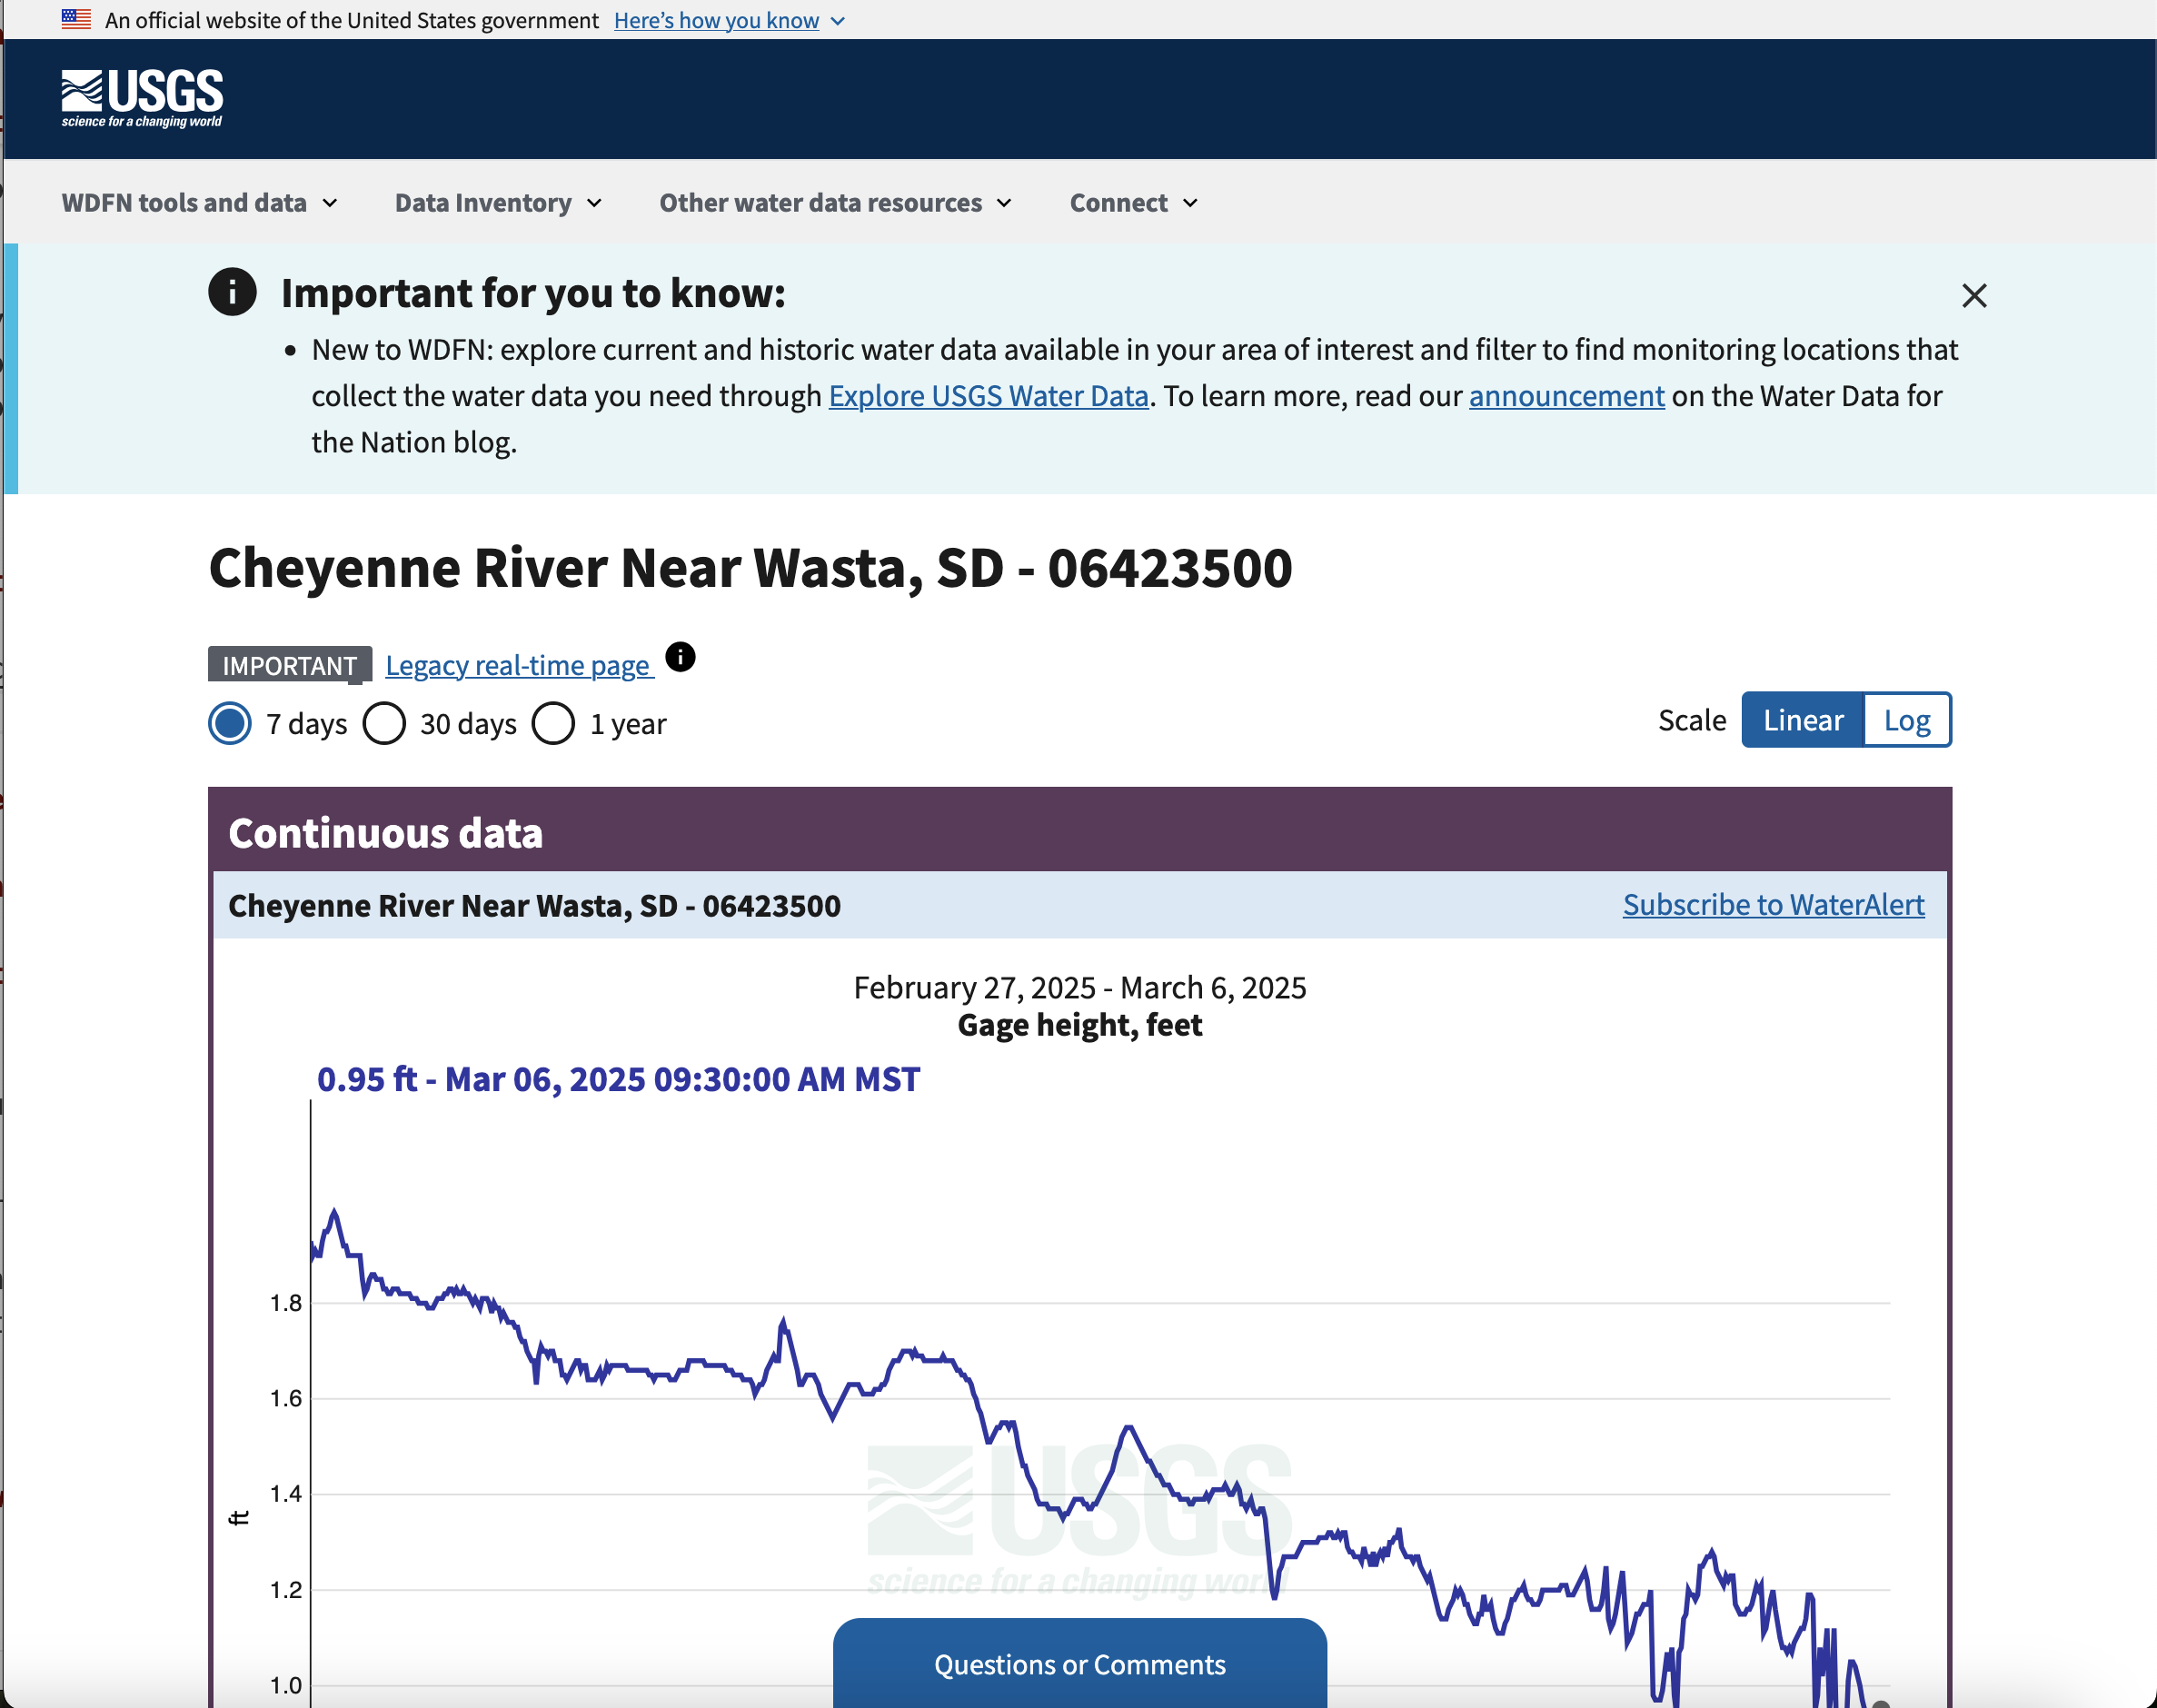
\includegraphics[keepaspectratio]{img/earth-analytics/flood-frequency/nwis-screenshots/11-preview-data.png}}

}

\caption{Return to the Cheyenne River near Wasta site page}

\end{figure}%

\subsubsection{Step 2: Data type}\label{step-2-data-type}

\begin{figure}[H]

{\centering \pandocbounded{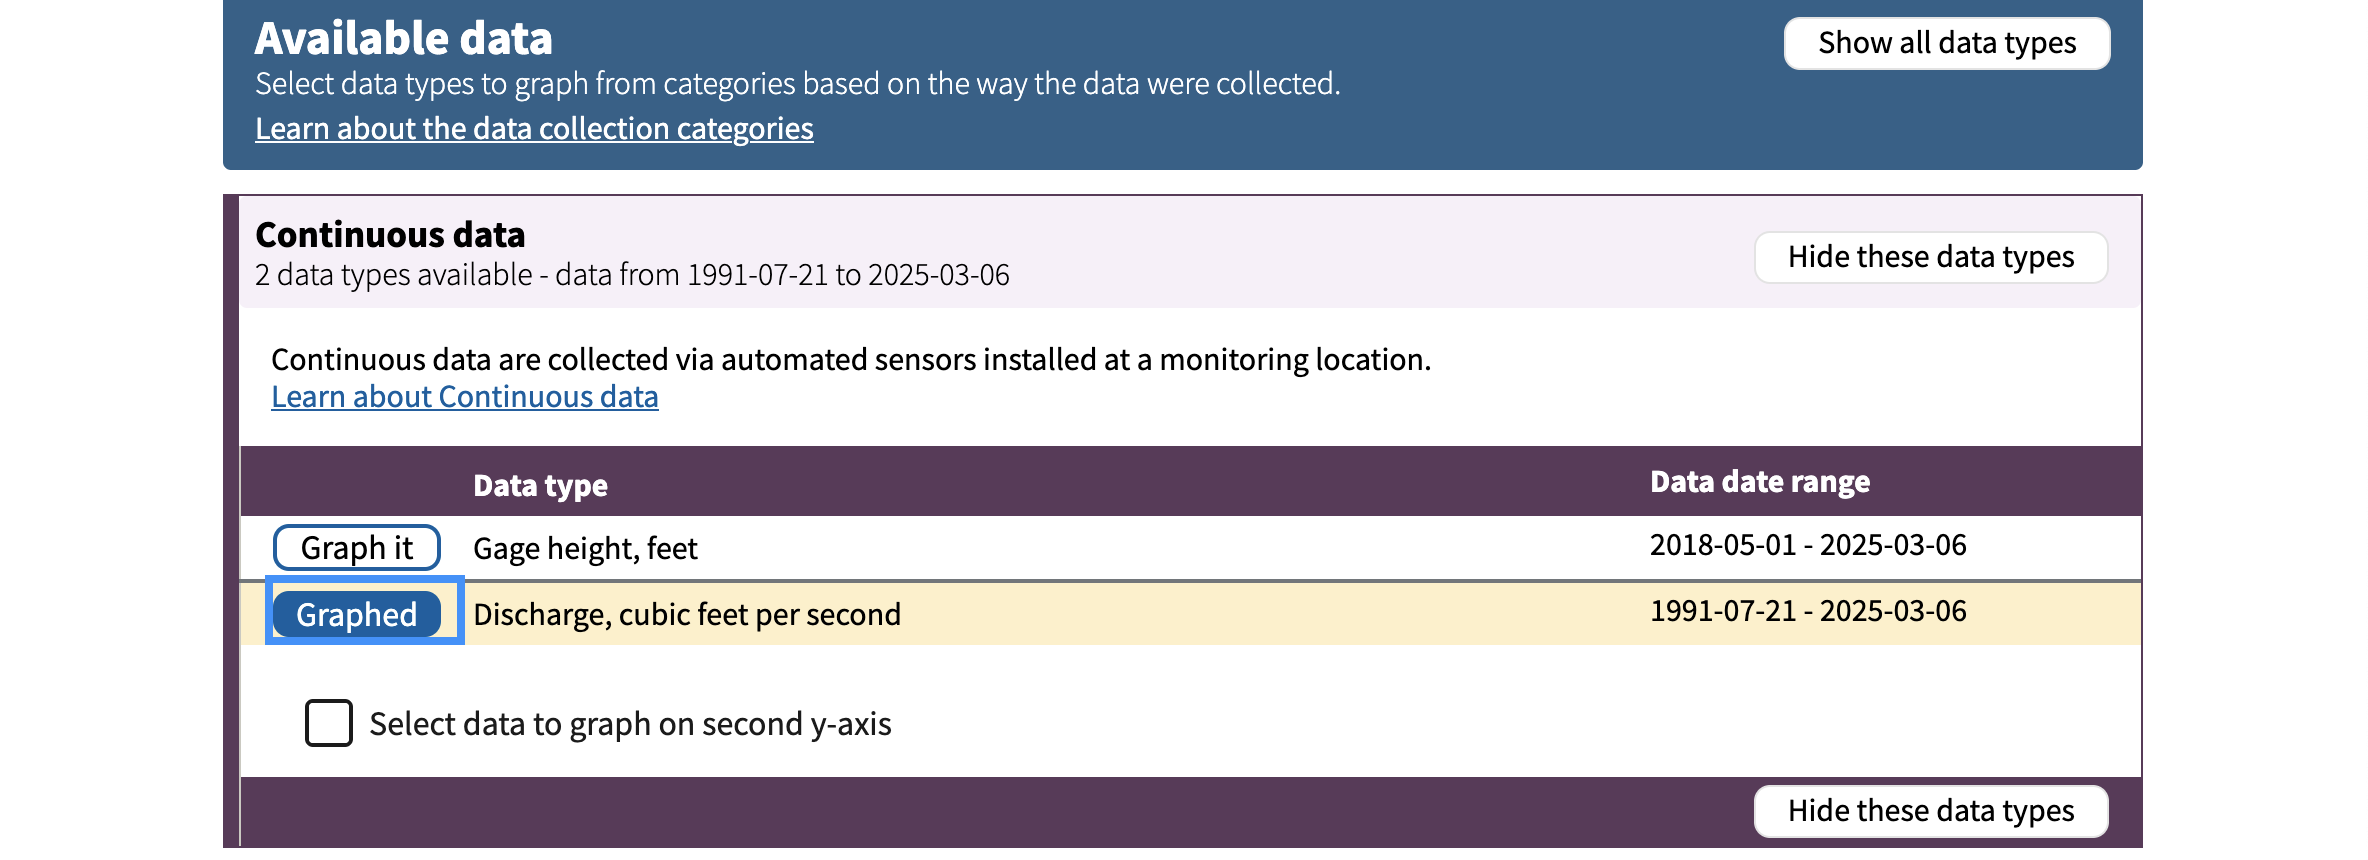
\includegraphics[keepaspectratio]{img/earth-analytics/flood-frequency/nwis-screenshots/12-data-type.png}}

}

\caption{Scroll down and switch the data type to Discharge instead of
Gage Height}

\end{figure}%

\subsubsection{Step 2: Change the plot
dates}\label{step-2-change-the-plot-dates}

\begin{figure}[H]

{\centering \pandocbounded{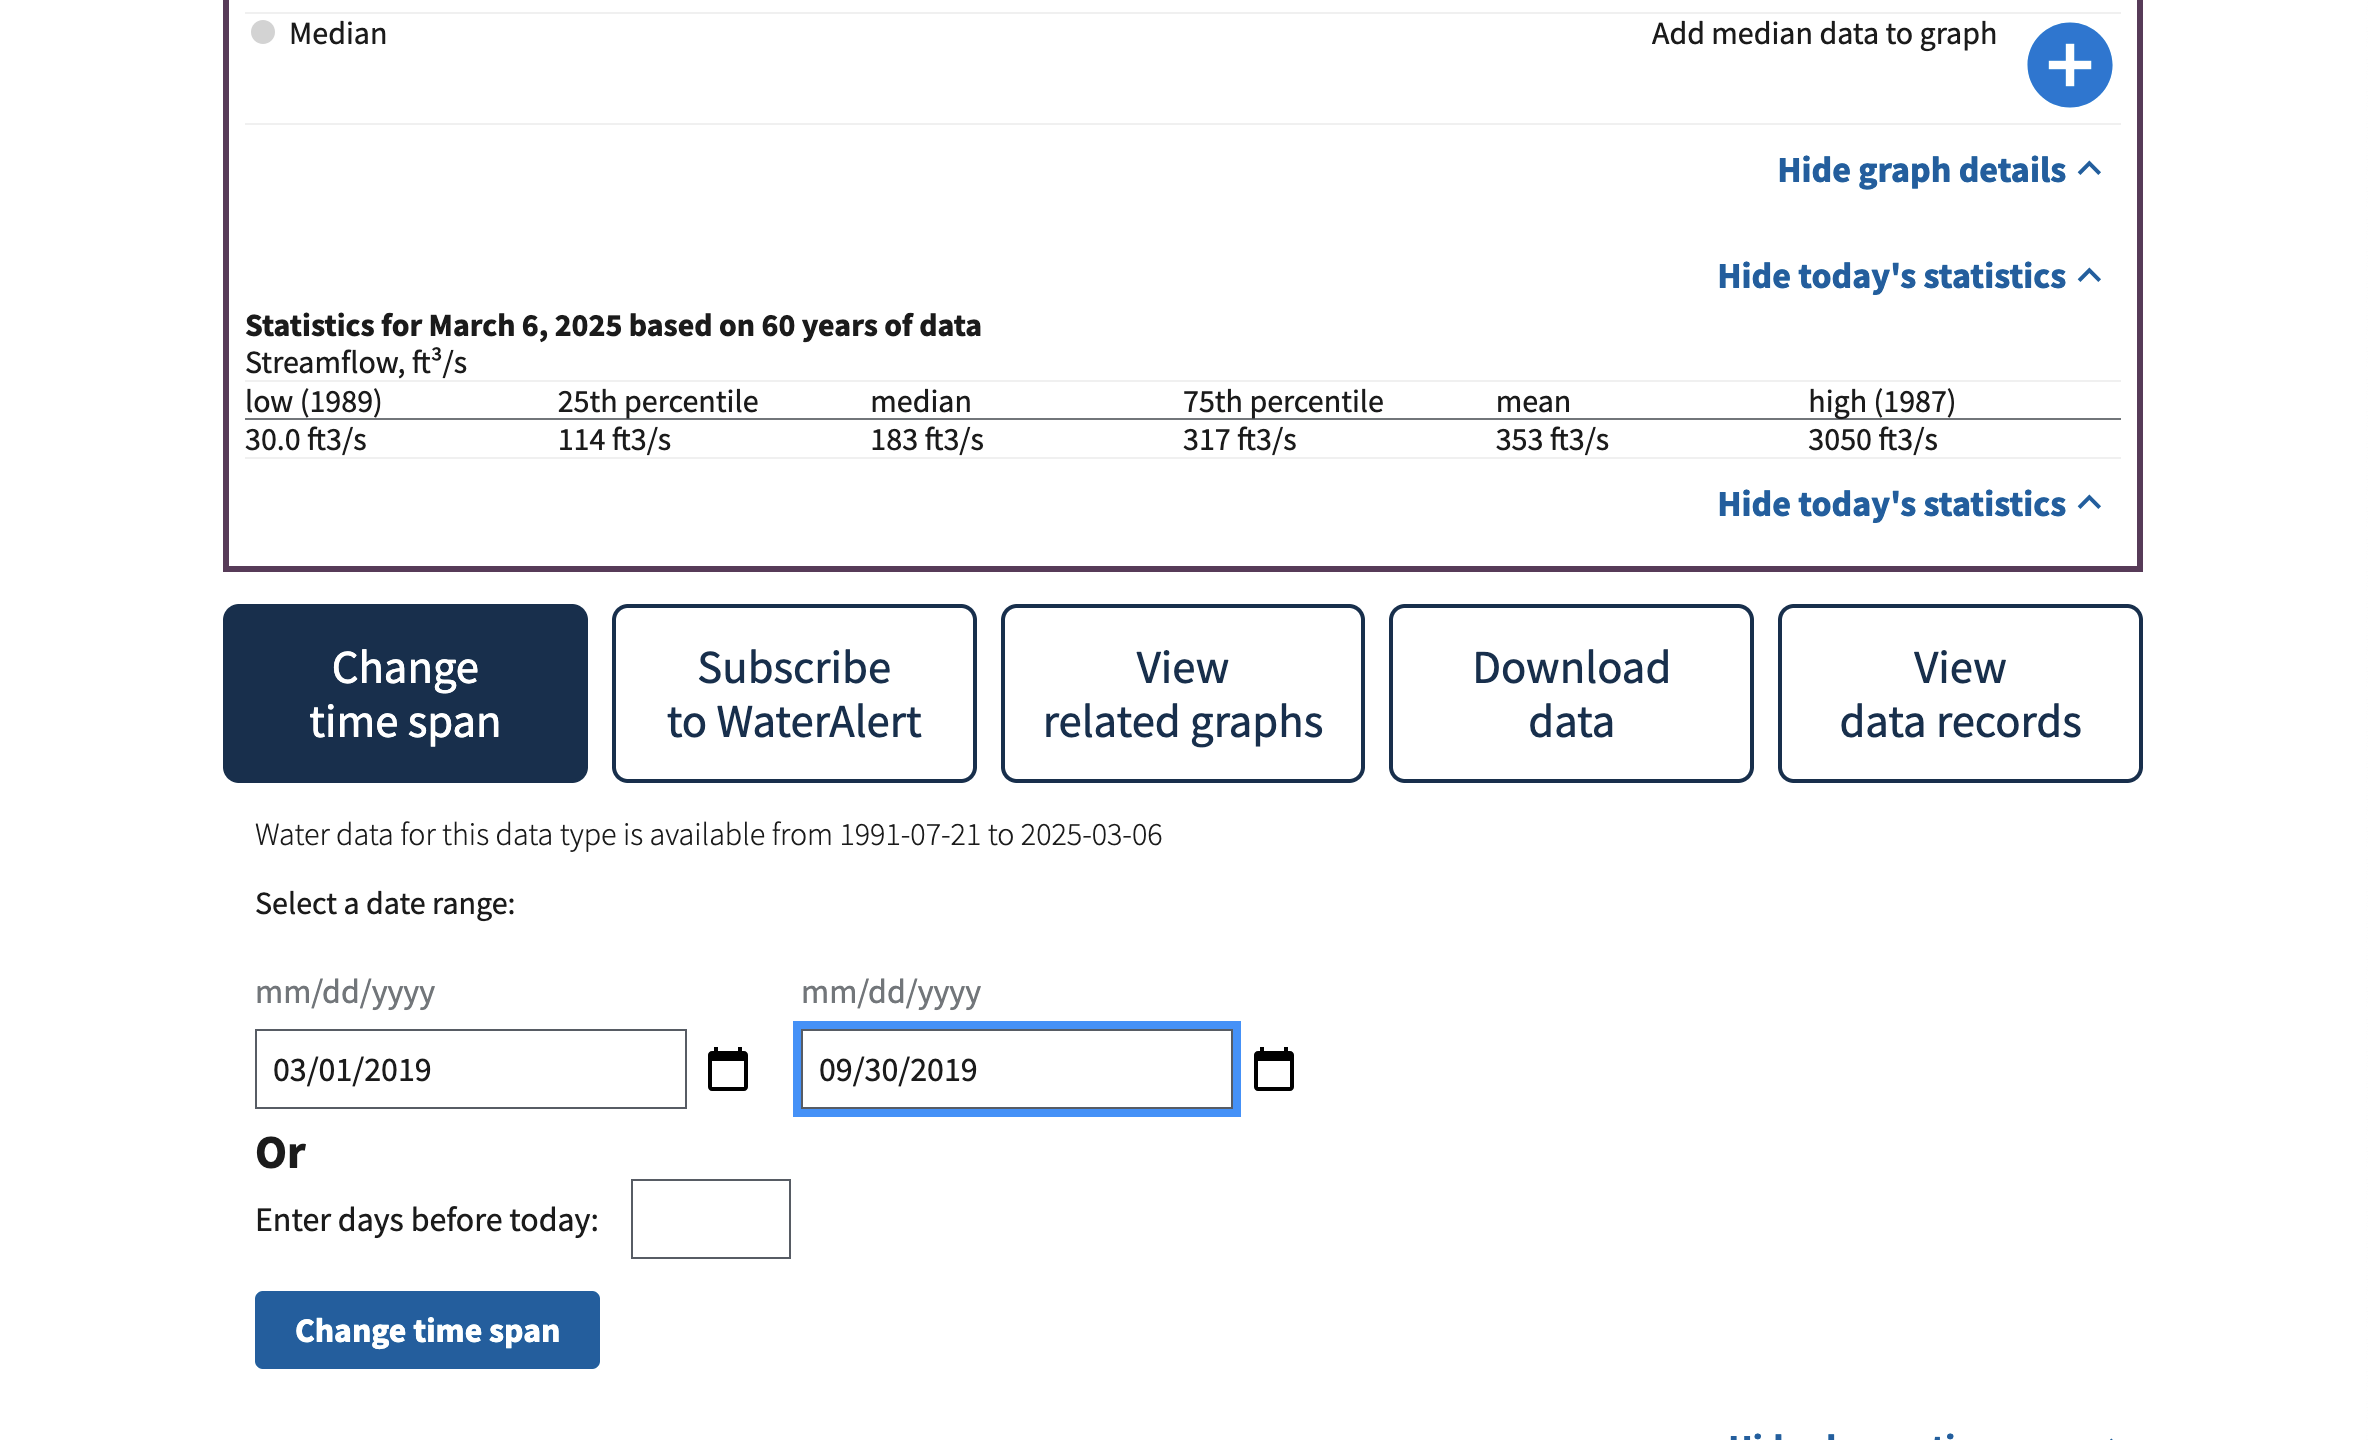
\includegraphics[keepaspectratio]{img/earth-analytics/flood-frequency/nwis-screenshots/13-dates.png}}

}

\caption{Scroll up and select the dates you want to look at.}

\end{figure}%

\subsubsection{Step 3: Look at the data}\label{step-3-look-at-the-data}

\begin{figure}[H]

{\centering \pandocbounded{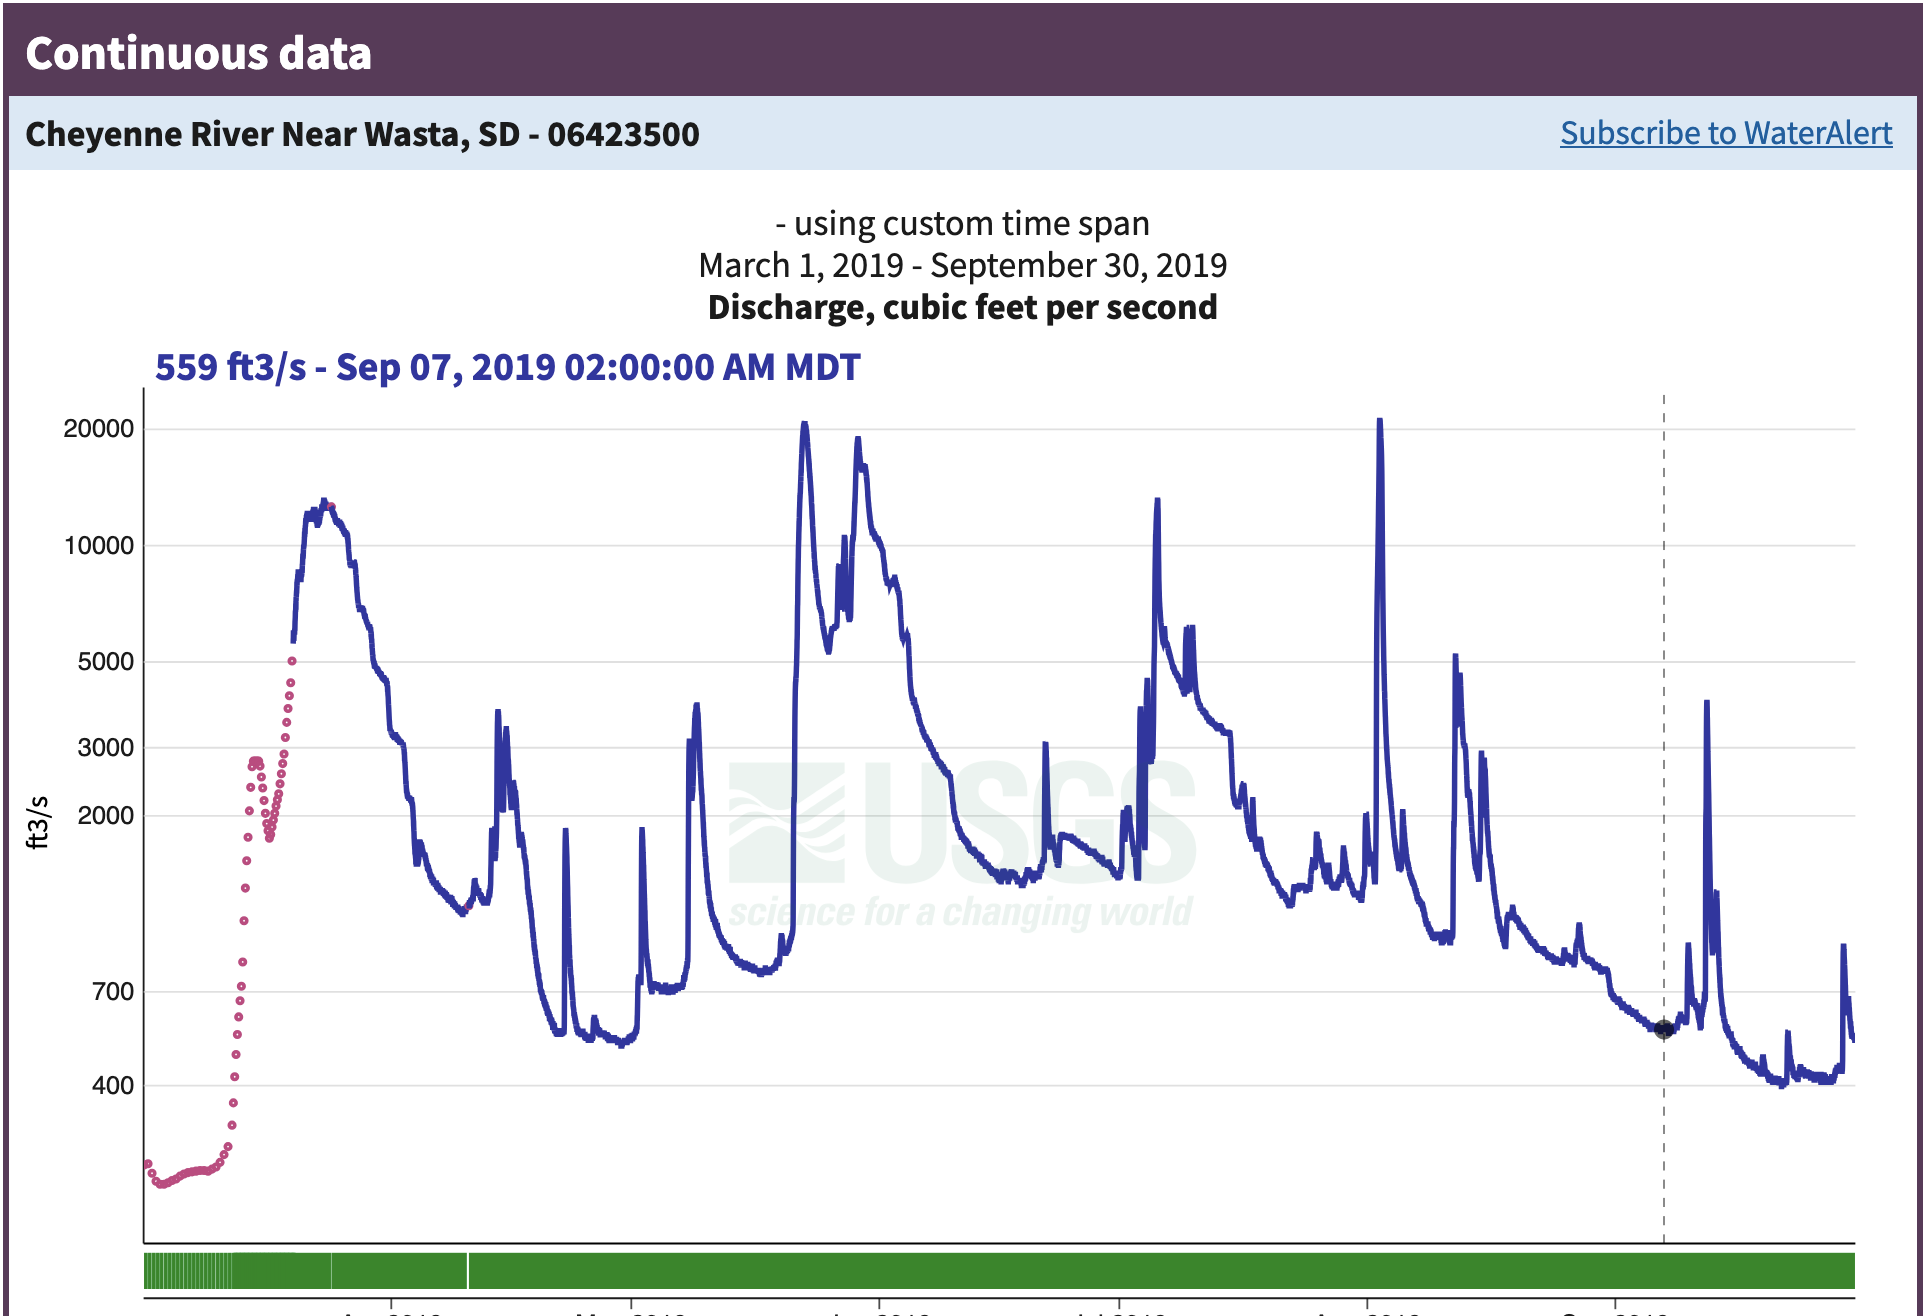
\includegraphics[keepaspectratio]{img/earth-analytics/flood-frequency/nwis-screenshots/14-finish.png}}

}

\caption{Take a look at your data. What do you see? You can try changing
some dates as well.}

\end{figure}%

\begin{tcolorbox}[enhanced jigsaw, colbacktitle=quarto-callout-color!10!white, opacityback=0, bottomtitle=1mm, toptitle=1mm, bottomrule=.15mm, left=2mm, colframe=quarto-callout-color-frame, leftrule=.75mm, opacitybacktitle=0.6, colback=white, rightrule=.15mm, toprule=.15mm, breakable, titlerule=0mm, title=\textcolor{quarto-callout-color}{\faInfo}\hspace{0.5em}{Reflect and Respond}, coltitle=black, arc=.35mm]

What do you notice about this data? You can think about:

\begin{itemize}
\tightlist
\item
  What type of data is it?
\item
  What dates in 2019 had the worst flooding?
\item
  How unusual were the 2019 floods?
\item
  Does anything about the data seem unusual to you?
\end{itemize}

\end{tcolorbox}

\subsubsection{Step 4: Look at some raw
data}\label{step-4-look-at-some-raw-data}

\pandocbounded{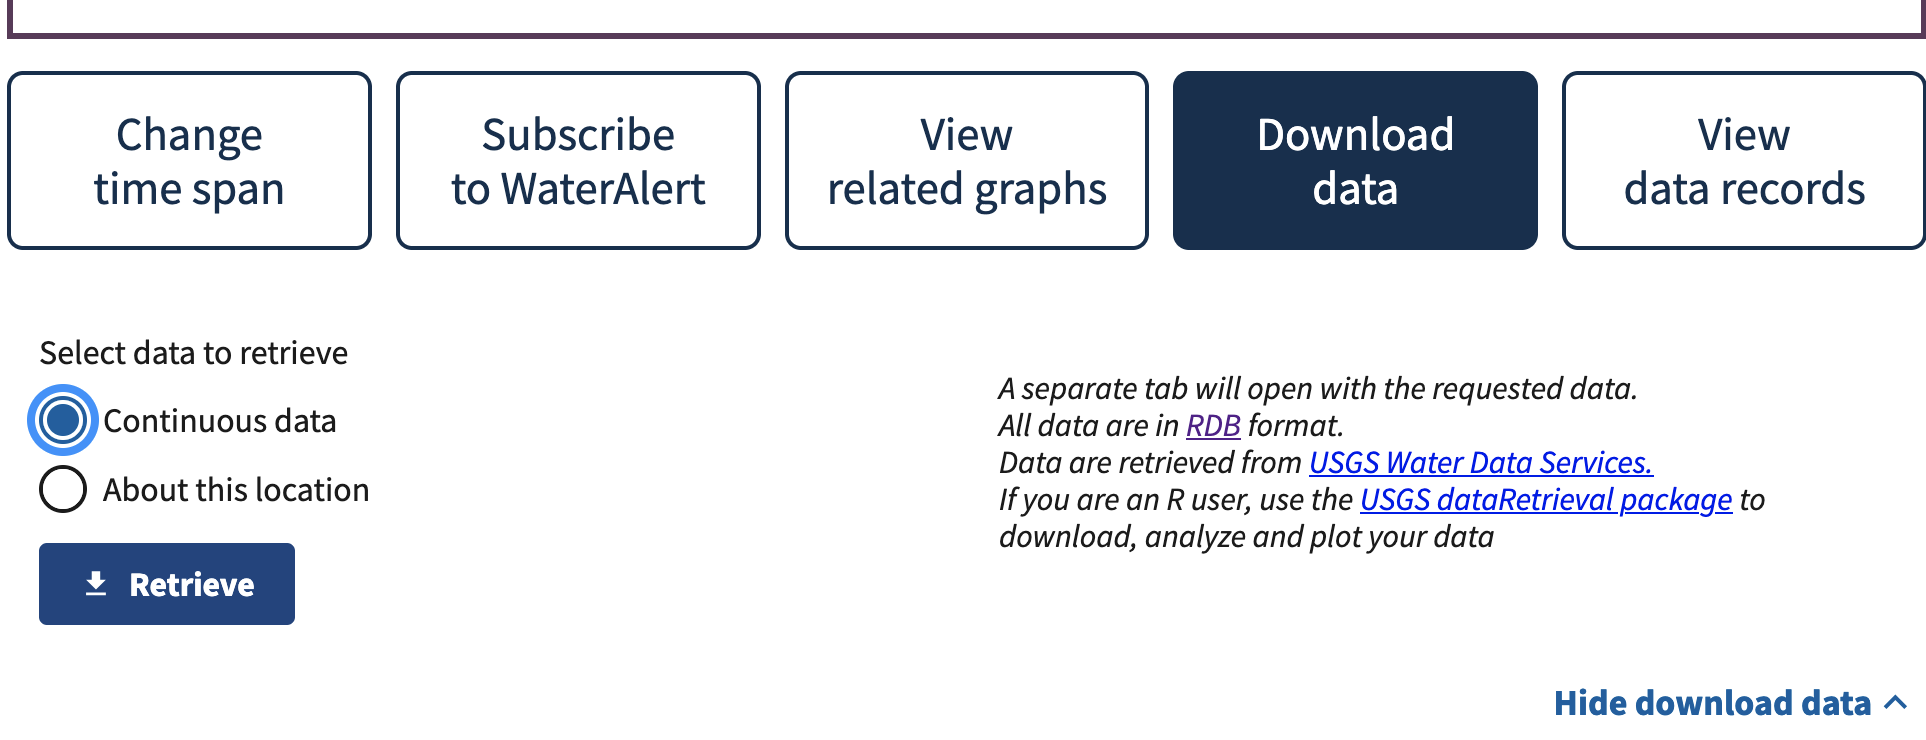
\includegraphics[keepaspectratio]{img/earth-analytics/flood-frequency/nwis-screenshots/15-download.png}}
Open up the file you downloaded -- it should automatically open in your
web browser. Does this look like streamflow data to you?

\begin{tcolorbox}[enhanced jigsaw, colbacktitle=quarto-callout-color!10!white, opacityback=0, bottomtitle=1mm, toptitle=1mm, bottomrule=.15mm, left=2mm, colframe=quarto-callout-color-frame, leftrule=.75mm, opacitybacktitle=0.6, colback=white, rightrule=.15mm, toprule=.15mm, breakable, titlerule=0mm, title=\textcolor{quarto-callout-color}{\faInfo}\hspace{0.5em}{Read More}, coltitle=black, arc=.35mm]

Check out the
\href{https://waterdata.usgs.gov/nwis/?tab_delimited_format_info}{NWIS
documentation} to find out more about how these data are formatted.

\end{tcolorbox}

\begin{tcolorbox}[enhanced jigsaw, colbacktitle=quarto-callout-color!10!white, opacityback=0, bottomtitle=1mm, toptitle=1mm, bottomrule=.15mm, left=2mm, colframe=quarto-callout-color-frame, leftrule=.75mm, opacitybacktitle=0.6, colback=white, rightrule=.15mm, toprule=.15mm, breakable, titlerule=0mm, title=\textcolor{quarto-callout-color}{\faInfo}\hspace{0.5em}{Reflect and Respond}, coltitle=black, arc=.35mm]

What do you notice about the data? Write down your thoughts on:

\begin{itemize}
\tightlist
\item
  What separator or \textbf{delimiter} does the data use to separate
  columns?
\item
  What should the data types of each column be?
\item
  Which column contains the streamflow data?
\item
  Do you need to skip any rows that don't contain data? How can you
  identify those rows?
\item
  Did you notice anything else?
\end{itemize}

\end{tcolorbox}

\subsection{Data description and
citation}\label{data-description-and-citation}

\begin{tcolorbox}[enhanced jigsaw, colbacktitle=quarto-callout-color!10!white, opacityback=0, bottomtitle=1mm, toptitle=1mm, bottomrule=.15mm, left=2mm, colframe=quarto-callout-color-frame, leftrule=.75mm, opacitybacktitle=0.6, colback=white, rightrule=.15mm, toprule=.15mm, breakable, titlerule=0mm, title=\textcolor{quarto-callout-color}{\faInfo}\hspace{0.5em}{Reflect and Respond}, coltitle=black, arc=.35mm]

Describe your data. Include the following information:

\begin{enumerate}
\def\labelenumi{\arabic{enumi}.}
\tightlist
\item
  A 1-2 sentence description of the data
\item
  Data citation
\item
  What are the units?
\item
  What is the time interval for each data point?
\item
  Is there a ``no data'' value, or a value used to indicate when the
  sensor was broken or didn't detect anything? (These are also known as
  NA, N/A, NaN, nan, or nodata values)
\end{enumerate}

\end{tcolorbox}

\section{Access the data with code}\label{access-the-data-with-code}

One way to access data is through an \textbf{Application Programming
Interface}, or \textbf{API}. Luckily for us, the USGS has written a
Python library to interface with the NWIS API, called
\texttt{dataretrieval}. The \texttt{dataretrieval.nwis}
\textbf{submodule} has a function or command for downloading stream
discharge data from the NWIS!

\begin{tcolorbox}[enhanced jigsaw, colbacktitle=quarto-callout-color!10!white, opacityback=0, bottomtitle=1mm, toptitle=1mm, bottomrule=.15mm, left=2mm, colframe=quarto-callout-color-frame, leftrule=.75mm, opacitybacktitle=0.6, colback=white, rightrule=.15mm, toprule=.15mm, breakable, titlerule=0mm, title=\textcolor{quarto-callout-color}{\faInfo}\hspace{0.5em}{Try It}, coltitle=black, arc=.35mm]

Import the \texttt{dataretrieval} library.

If you want to store the data so that you are not dependant on the API
to keep working, you will also need the \texttt{earthpy} library for
managing local files and the \texttt{pandas} library for loading a
\texttt{csv} file. If you are going that route, import the libraries you
need, making sure to follow PEP-8 guidelines by keeping your libraries
in alphabetical order.

\end{tcolorbox}

\begin{Shaded}
\begin{Highlighting}[]
\CommentTok{\# Import libraries}
\end{Highlighting}
\end{Shaded}

Next, we'll set some parameters. You can use these to customize your
workflow.

\begin{Shaded}
\begin{Highlighting}[]
\BuiltInTok{id} \OperatorTok{=} \StringTok{\textquotesingle{}stars\textquotesingle{}}
\NormalTok{site\_name }\OperatorTok{=} \StringTok{\textquotesingle{}Cheyenne River\textquotesingle{}}
\NormalTok{year }\OperatorTok{=} \DecValTok{2019}
\NormalTok{data\_dir }\OperatorTok{=} \StringTok{\textquotesingle{}cheyenne{-}river{-}flood\textquotesingle{}}
\NormalTok{download\_title }\OperatorTok{=} \StringTok{\textquotesingle{}Cheyenne River Flood Frequency\textquotesingle{}}
\NormalTok{csv\_filename }\OperatorTok{=} \StringTok{\textquotesingle{}cheyenne\_streamflow\_1934\_2024.csv\textquotesingle{}}
\end{Highlighting}
\end{Shaded}

\begin{tcolorbox}[enhanced jigsaw, colbacktitle=quarto-callout-color!10!white, opacityback=0, bottomtitle=1mm, toptitle=1mm, bottomrule=.15mm, left=2mm, colframe=quarto-callout-color-frame, leftrule=.75mm, opacitybacktitle=0.6, colback=white, rightrule=.15mm, toprule=.15mm, breakable, titlerule=0mm, title=\textcolor{quarto-callout-color}{\faInfo}\hspace{0.5em}{Try It}, coltitle=black, arc=.35mm]

The sample code below needs some changes from you before it will run.

\begin{enumerate}
\def\labelenumi{\arabic{enumi}.}
\tightlist
\item
  Find the site number on the site page for the Cheyenne River near
  Wasta gage.
\item
  Determine what date range you would like to download. For right now,
  start by downloading just the data
\item
  Define variables for the site number, start date, and end date to
  match the rest of the code. You can find the site number on the site
  page.
\item
  Download the data using the provided code.
\end{enumerate}

Note that the \texttt{dataretrieval.nwis.get\_discharge\_measurements()}
function returns data in a format called a \texttt{pandas}
\texttt{DataFrame}, as well as metadata in a format called a
\texttt{NWIS\_metadata}. That's why we need two variables to store the
results.

\end{tcolorbox}

\begin{tcolorbox}[enhanced jigsaw, colbacktitle=quarto-callout-color!10!white, opacityback=0, bottomtitle=1mm, toptitle=1mm, bottomrule=.15mm, left=2mm, colframe=quarto-callout-color-frame, leftrule=.75mm, opacitybacktitle=0.6, colback=white, rightrule=.15mm, toprule=.15mm, breakable, titlerule=0mm, title=\textcolor{quarto-callout-color}{\faInfo}\hspace{0.5em}{Looking for an Extra Challenge?}, coltitle=black, arc=.35mm]

Try to write some code:

\begin{enumerate}
\def\labelenumi{\arabic{enumi}.}
\tightlist
\item
  Store the data on your computer
\item
  Only download the data if it's not on the computer already.
\item
  Load the data from your computer.
\end{enumerate}

\end{tcolorbox}

\begin{tcolorbox}[enhanced jigsaw, colbacktitle=quarto-callout-tip-color!10!white, opacityback=0, bottomtitle=1mm, toptitle=1mm, bottomrule=.15mm, left=2mm, colframe=quarto-callout-tip-color-frame, leftrule=.75mm, opacitybacktitle=0.6, colback=white, rightrule=.15mm, toprule=.15mm, breakable, titlerule=0mm, title=\textcolor{quarto-callout-tip-color}{\faLightbulb}\hspace{0.5em}{Water Years}, coltitle=black, arc=.35mm]

When we look at streamflow data, we usually try to download
\textbf{water years} rather than calendar years. The water year in the
Northern Hemisphere starts on October 1 of the previous calendar year
and runs through September 31. For example, water year 2018 (or WY2018)
runs from October 1, 2017 to September 31, 2018.

Why is the water year different? In most of the Northern Hemisphere, the
snowpack is as low as it gets around October 1, and begins to build up
for the winter at that point. When we're keeping track of water fluxes,
it's easiest if we don't need a count on how much water is in the snow
pack at the start of the year.

\end{tcolorbox}

\begin{tcolorbox}[enhanced jigsaw, colbacktitle=quarto-callout-color!10!white, opacityback=0, bottomtitle=1mm, toptitle=1mm, bottomrule=.15mm, left=2mm, colframe=quarto-callout-color-frame, leftrule=.75mm, opacitybacktitle=0.6, colback=white, rightrule=.15mm, toprule=.15mm, breakable, titlerule=0mm, title=\textcolor{quarto-callout-color}{\faInfo}\hspace{0.5em}{Reflect and Respond}, coltitle=black, arc=.35mm]

What parameter would you change in the code below if you wanted to
switch locations?

\end{tcolorbox}

\begin{Shaded}
\begin{Highlighting}[]
\CommentTok{\# Define download parameters HERE}

\CommentTok{\# Get discharge data and metadata from NWIS}
\NormalTok{nwis\_df, meta }\OperatorTok{=}\NormalTok{ dataretrieval.nwis.get\_discharge\_measurements(}
\NormalTok{    sites}\OperatorTok{=}\NormalTok{site\_number,}
\NormalTok{    start}\OperatorTok{=}\NormalTok{start\_date,}
\NormalTok{    end}\OperatorTok{=}\NormalTok{end\_date)}
\NormalTok{nwis\_df}
\end{Highlighting}
\end{Shaded}

Now, let's check the data:

\begin{Shaded}
\begin{Highlighting}[]
\NormalTok{nwis\_df.info()}
\end{Highlighting}
\end{Shaded}

\begin{verbatim}
<class 'pandas.core.frame.DataFrame'>
DatetimeIndex: 32866 entries, 1934-10-01 00:00:00+00:00 to 2024-09-30 00:00:00+00:00
Data columns (total 5 columns):
 #   Column         Non-Null Count  Dtype  
---  ------         --------------  -----  
 0   site_no        32866 non-null  int64  
 1   00060_Mean     32866 non-null  float64
 2   00060_Mean_cd  32866 non-null  object 
 3   00065_Mean     1592 non-null   float64
 4   00065_Mean_cd  1592 non-null   object 
dtypes: float64(2), int64(1), object(2)
memory usage: 1.5+ MB
\end{verbatim}

The \texttt{dataretrieval} library has taken care of a lot of the work
of accessing and importing NWIS data. However, we still want to clean up
the data a little, by selecting the column we want and renaming it with
a descriptive label. You should also double-check that any
\texttt{NODATA} values are properly encoded, and that the data types
make sense! For example, plotting a histogram can be a useful way to see
if the data values are what you expect.

\begin{tcolorbox}[enhanced jigsaw, colbacktitle=quarto-callout-color!10!white, opacityback=0, bottomtitle=1mm, toptitle=1mm, bottomrule=.15mm, left=2mm, colframe=quarto-callout-color-frame, leftrule=.75mm, opacitybacktitle=0.6, colback=white, rightrule=.15mm, toprule=.15mm, breakable, titlerule=0mm, title=\textcolor{quarto-callout-color}{\faInfo}\hspace{0.5em}{Reflect and Respond}, coltitle=black, arc=.35mm]

Do you see any problems with your data? List out three things that you
checked to make sure that you won't have problems down the line.

\end{tcolorbox}

\bookmarksetup{startatroot}

\chapter{Spring returns to the Great
Plains}\label{spring-returns-to-the-great-plains}

Mapping Tasiyagnunpa migration

\hfill\break

Tasiyagnunpa (or Western Meadowlark, or \emph{sturnella neglecta})
migrates each year to nest on the Great Plains in the United States.
Using crowd-sourced observations of these birds, we can see that
migration happening throughout the year.

\begin{figure}[H]

{\centering \pandocbounded{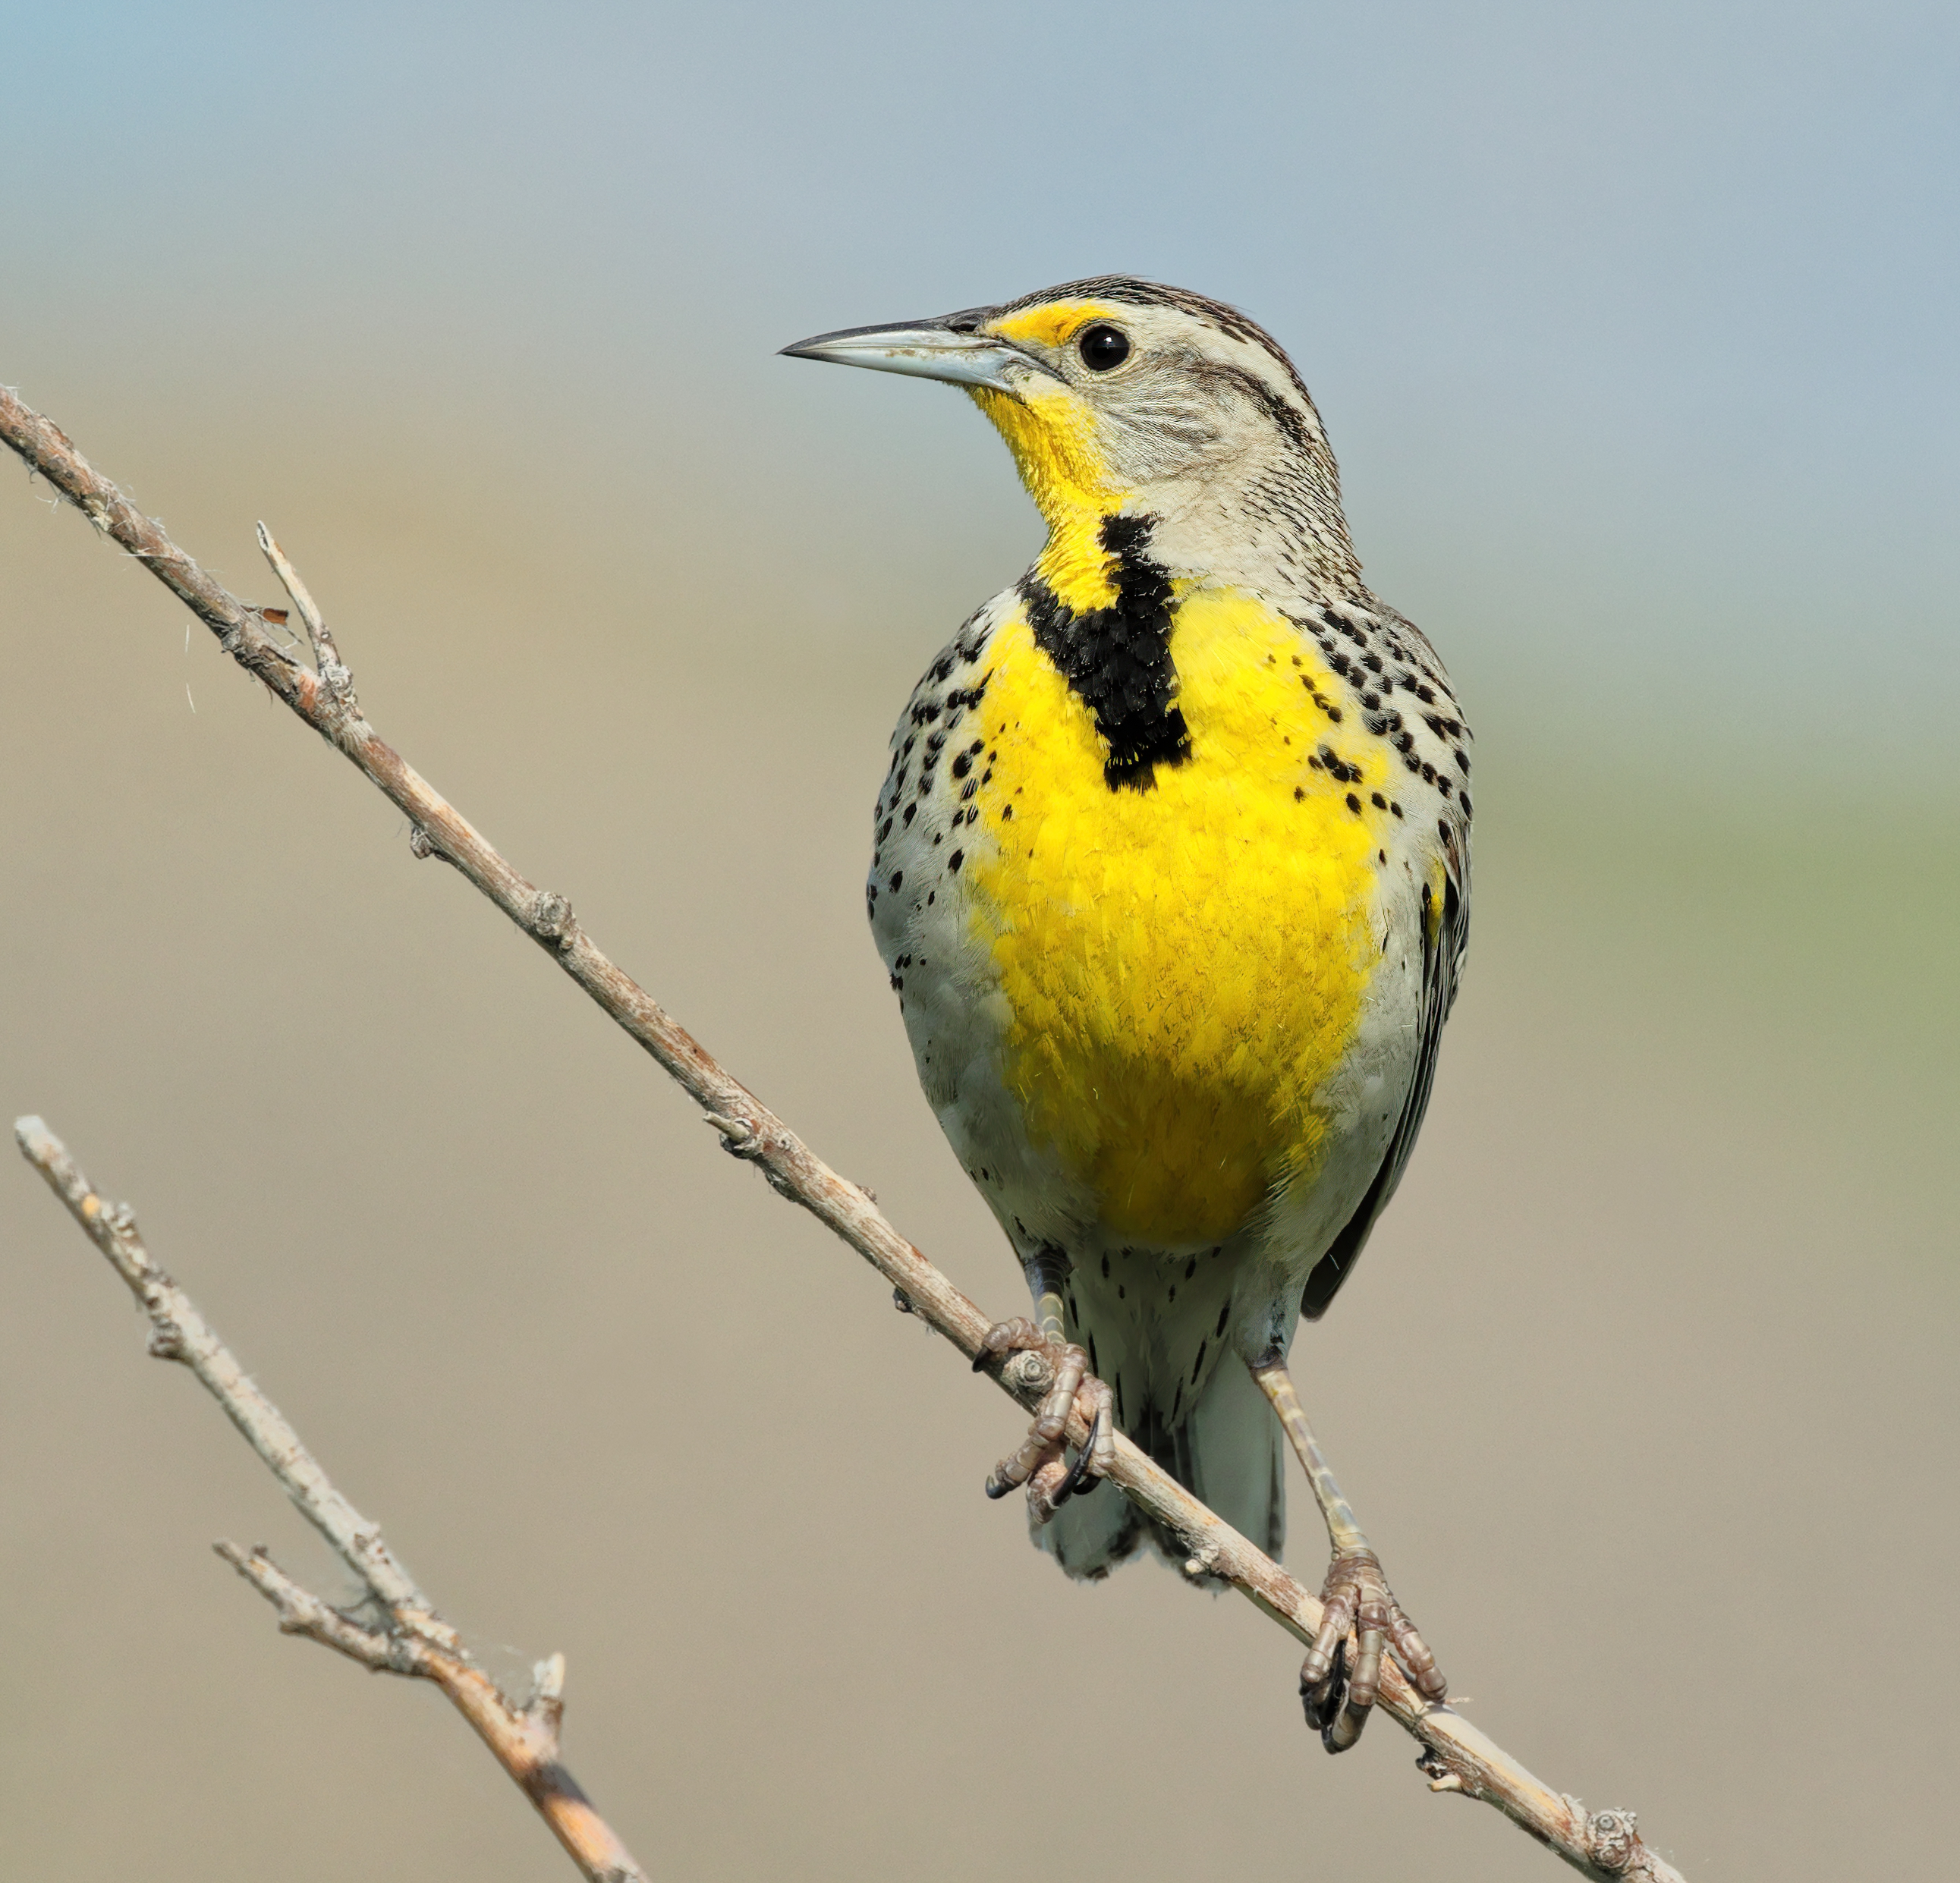
\includegraphics[keepaspectratio]{img/notebooks/migration/sturnella_neglecta.jpg}}

}

\caption{Western meadowlark (Sturnella neglecta), Grasslands National
Park, Saskatchewan, Canada from Cephas, CC BY-SA 4.0
\url{https://creativecommons.org/licenses/by-sa/4.0}, via Wikimedia
Commons url
https://commons.wikimedia.org/wiki/File:Sturnella\_neglecta\_GNP\_02.jpg)}

\end{figure}%

\begin{tcolorbox}[enhanced jigsaw, colbacktitle=quarto-callout-color!10!white, opacityback=0, bottomtitle=1mm, toptitle=1mm, bottomrule=.15mm, left=2mm, colframe=quarto-callout-color-frame, leftrule=.75mm, opacitybacktitle=0.6, colback=white, rightrule=.15mm, toprule=.15mm, breakable, titlerule=0mm, title=\textcolor{quarto-callout-color}{\faInfo}\hspace{0.5em}{Read More}, coltitle=black, arc=.35mm]

Read more about the Lakota connection to Tasiyagnunpa from
\href{https://www.nativesunnews.today/articles/meadowlarks-still-speak-lakota-humans-dont-anymore/}{Native
Sun News Today}

\end{tcolorbox}

\begin{tcolorbox}[enhanced jigsaw, colbacktitle=quarto-callout-color!10!white, opacityback=0, bottomtitle=1mm, toptitle=1mm, bottomrule=.15mm, left=2mm, colframe=quarto-callout-color-frame, leftrule=.75mm, opacitybacktitle=0.6, colback=white, rightrule=.15mm, toprule=.15mm, breakable, titlerule=0mm, title=\textcolor{quarto-callout-color}{\faInfo}\hspace{0.5em}{Check out our demo video!}, coltitle=black, arc=.35mm]

\subsection{Prepare Data}

DEMO: Migration Part 1 (EDA) by Earth Lab

\subsection{Dynamic Plot}

DEMO: Migration Part 2 (EDA) by Earth Lab

\subsection{Portfolio Post}

\end{tcolorbox}

Reflect on what you know about migration. You could consider:

\begin{enumerate}
\def\labelenumi{\arabic{enumi}.}
\tightlist
\item
  What are some reasons that animals migrate?
\item
  How might climate change affect animal migrations?
\item
  Do you notice any animal migrations in your area?
\end{enumerate}

Before we get started, let's define some parameters for the workflow.
We'll use these throughout to customize the workflow for this species:

\begin{Shaded}
\begin{Highlighting}[]
\BuiltInTok{id} \OperatorTok{=} \StringTok{\textquotesingle{}stars\textquotesingle{}}
\NormalTok{project\_title }\OperatorTok{=} \StringTok{\textquotesingle{}Tasiyagnunpa Migration 2023\textquotesingle{}}
\NormalTok{species\_name }\OperatorTok{=} \StringTok{\textquotesingle{}Tasiyagnunpa\textquotesingle{}}
\NormalTok{species\_lookup }\OperatorTok{=} \StringTok{\textquotesingle{}sturnella neglecta\textquotesingle{}}
\NormalTok{species\_key }\OperatorTok{=} \DecValTok{9596413}
\NormalTok{year }\OperatorTok{=} \DecValTok{2023}
\NormalTok{gbif\_filename }\OperatorTok{=} \StringTok{\textquotesingle{}gbif\_tasiyagnunpa.csv\textquotesingle{}}
\NormalTok{ecoregions\_dir }\OperatorTok{=} \StringTok{\textquotesingle{}wwf\_ecoregions\textquotesingle{}}
\NormalTok{plot\_filename }\OperatorTok{=} \StringTok{\textquotesingle{}tasiyagnunpa\_migration\textquotesingle{}}
\NormalTok{plot\_height }\OperatorTok{=} \DecValTok{500}
\end{Highlighting}
\end{Shaded}

\section{STEP 1: Set up your reproducible
workflow}\label{step-1-set-up-your-reproducible-workflow}

\subsection{Import Python libraries}\label{import-python-libraries}

\begin{tcolorbox}[enhanced jigsaw, colbacktitle=quarto-callout-color!10!white, opacityback=0, bottomtitle=1mm, toptitle=1mm, bottomrule=.15mm, left=2mm, colframe=quarto-callout-color-frame, leftrule=.75mm, opacitybacktitle=0.6, colback=white, rightrule=.15mm, toprule=.15mm, breakable, titlerule=0mm, title=\textcolor{quarto-callout-color}{\faInfo}\hspace{0.5em}{Try It: Import packages}, coltitle=black, arc=.35mm]

In the imports cell, we've included some packages that you will need.
Add imports for packages that will help you:

\begin{enumerate}
\def\labelenumi{\arabic{enumi}.}
\tightlist
\item
  Work with tabular data
\item
  Work with geospatial vector data
\end{enumerate}

\end{tcolorbox}

\begin{Shaded}
\begin{Highlighting}[]
\ImportTok{import}\NormalTok{ os}
\ImportTok{import}\NormalTok{ pathlib}

\ImportTok{import}\NormalTok{ earthpy}
\end{Highlighting}
\end{Shaded}

\subsection{Create a directory for your
data}\label{create-a-directory-for-your-data}

For this challenge, you will need to download some data to the computer
you're working on. We suggest using the \texttt{earthpy} library we
develop to manage your downloads, since it encapsulates many best
practices as far as:

\begin{enumerate}
\def\labelenumi{\arabic{enumi}.}
\tightlist
\item
  Where to store your data
\item
  Dealing with archived data like .zip files
\item
  Avoiding version control problems
\item
  Making sure your code works cross-platform
\item
  Avoiding duplicate downloads
\end{enumerate}

If you're working on one of our assignments through GitHub Classroom, it
also lets us build in some handy defaults so that you can see your data
files while you work.

\begin{tcolorbox}[enhanced jigsaw, colbacktitle=quarto-callout-color!10!white, opacityback=0, bottomtitle=1mm, toptitle=1mm, bottomrule=.15mm, left=2mm, colframe=quarto-callout-color-frame, leftrule=.75mm, opacitybacktitle=0.6, colback=white, rightrule=.15mm, toprule=.15mm, breakable, titlerule=0mm, title=\textcolor{quarto-callout-color}{\faInfo}\hspace{0.5em}{Try It: Create a project folder}, coltitle=black, arc=.35mm]

The code below will help you get started with making a project directory

\begin{enumerate}
\def\labelenumi{\arabic{enumi}.}
\tightlist
\item
  Replace
  \texttt{\textquotesingle{}your-project-directory-name-here\textquotesingle{}}
  with a \textbf{descriptive} name
\item
  Run the cell
\item
  The code should have printed out the path to your data files. Check
  that your data directory exists and has data in it using the terminal
  or your Finder/File Explorer.
\end{enumerate}

\end{tcolorbox}

\begin{tcolorbox}[enhanced jigsaw, colbacktitle=quarto-callout-tip-color!10!white, opacityback=0, bottomtitle=1mm, toptitle=1mm, bottomrule=.15mm, left=2mm, colframe=quarto-callout-tip-color-frame, leftrule=.75mm, opacitybacktitle=0.6, colback=white, rightrule=.15mm, toprule=.15mm, breakable, titlerule=0mm, title=\textcolor{quarto-callout-tip-color}{\faLightbulb}\hspace{0.5em}{File structure}, coltitle=black, arc=.35mm]

These days, a lot of people find your file by searching for them or
selecting from a \texttt{Bookmarks} or \texttt{Recents} list. Even if
you don't use it, your computer also keeps files in a \textbf{tree}
structure of folders. Put another way, you can organize and find files
by travelling along a unique \textbf{path}, e.g.~\texttt{My\ Drive}
\textgreater{} \texttt{Documents} \textgreater{}
\texttt{My\ awesome\ project} \textgreater{} \texttt{A\ project\ file}
where each subsequent folder is \textbf{inside} the previous one. This
is convenient because all the files for a project can be in the same
place, and both people and computers can rapidly locate files they want,
provided they remember the path.

You may notice that when Python prints out a file path like this, the
folder names are \textbf{separated} by a \texttt{/} or
\texttt{\textbackslash{}} (depending on your operating system). This
character is called the \textbf{file separator}, and it tells you that
the next piece of the path is \textbf{inside} the previous one.

\end{tcolorbox}

\begin{Shaded}
\begin{Highlighting}[]
\CommentTok{\# Create data directory}
\NormalTok{project }\OperatorTok{=}\NormalTok{ earthpy.Project(}
\NormalTok{    title}\OperatorTok{=}\NormalTok{project\_title,}
\NormalTok{    dirname}\OperatorTok{=}\StringTok{\textquotesingle{}your{-}project{-}directory{-}name{-}here\textquotesingle{}}\NormalTok{)}
\CommentTok{\# Download sample data}
\NormalTok{project.get\_data()}

\CommentTok{\# Display the project directory}
\NormalTok{project.project\_dir}
\end{Highlighting}
\end{Shaded}

\section{STEP 2: Define your study area -- the ecoregions of North
America}\label{step-2-define-your-study-area-the-ecoregions-of-north-america}

Your sample data package included a Shapefile of global
\textbf{ecoregions}. You should be able to see changes in the number of
observations of \textbf{?meta:params.species\_name} in each ecoregion
throughout the year.

\marginnote{\begin{footnotesize}

You don't have to use ecoregions to group species observations -- you
could choose to use political boundaries like countries or states, other
natural boundaries like watersheds, or even uniform hexagonal areas as
is common in conservation work. We chose ecoregions because we expect
the suitability for a species at a particular time of year to be
relatively consistent across the region.

\end{footnotesize}}

\begin{tcolorbox}[enhanced jigsaw, colbacktitle=quarto-callout-color!10!white, opacityback=0, bottomtitle=1mm, toptitle=1mm, bottomrule=.15mm, left=2mm, colframe=quarto-callout-color-frame, leftrule=.75mm, opacitybacktitle=0.6, colback=white, rightrule=.15mm, toprule=.15mm, breakable, titlerule=0mm, title=\textcolor{quarto-callout-color}{\faInfo}\hspace{0.5em}{Read More}, coltitle=black, arc=.35mm]

The ecoregion data will be available as a \textbf{shapefile}. Learn more
about shapefiles and vector data in this
\href{https://www.earthdatascience.org/courses/intro-to-earth-data-science/file-formats/use-spatial-data/use-vector-data/}{Introduction
to Spatial Vector Data File Formats in Open Source Python}

\end{tcolorbox}

\subsection{Load the ecoregions into
Python}\label{load-the-ecoregions-into-python}

\begin{tcolorbox}[enhanced jigsaw, colbacktitle=quarto-callout-color!10!white, opacityback=0, bottomtitle=1mm, toptitle=1mm, bottomrule=.15mm, left=2mm, colframe=quarto-callout-color-frame, leftrule=.75mm, opacitybacktitle=0.6, colback=white, rightrule=.15mm, toprule=.15mm, breakable, titlerule=0mm, title=\textcolor{quarto-callout-color}{\faInfo}\hspace{0.5em}{Try It: Load ecoregions into Python}, coltitle=black, arc=.35mm]

Download and save ecoregion boundaries from the EPA:

\begin{enumerate}
\def\labelenumi{\arabic{enumi}.}
\tightlist
\item
  Replace \texttt{a\_path} with the path your created for your
  ecoregions file.
\item
  (optional) Consider renaming and selecting columns to make your
  \texttt{GeoDataFrame} easier to work with. Many of the same methods
  you learned for \texttt{pandas} \texttt{DataFrame}s are the same for
  \texttt{GeoDataFrame}s! NOTE: Make sure to keep the
  \texttt{\textquotesingle{}SHAPE\_AREA\textquotesingle{}} column around
  -- we will need that later!
\item
  Make a quick plot with \texttt{.plot()} to make sure the download
  worked.
\item
  Run the cell to load the data into Python
\end{enumerate}

\end{tcolorbox}

\begin{Shaded}
\begin{Highlighting}[]
\CommentTok{\# Open up the ecoregions boundaries}
\NormalTok{gdf }\OperatorTok{=}\NormalTok{ gpd.read\_file(a\_path)}

\CommentTok{\# Name the index so it will match the other data later on}
\NormalTok{gdf.index.name }\OperatorTok{=} \StringTok{\textquotesingle{}ecoregion\textquotesingle{}}

\CommentTok{\# Plot the ecoregions quickly to check download}
\end{Highlighting}
\end{Shaded}

\section{STEP 3: Load species observation
data}\label{step-3-load-species-observation-data}

For this challenge, you will use a database called the
\href{https://www.gbif.org/}{Global Biodiversity Information Facility
(GBIF)}. GBIF is compiled from species observation data all over the
world, and includes everything from museum specimens to photos taken by
citizen scientists in their backyards. We've compiled some sample data
in the same format that you will get from GBIF.

Let's start by looking at a little of the raw data.

\begin{Shaded}
\begin{Highlighting}[]
\NormalTok{gbif\_path }\OperatorTok{=}\NormalTok{ project.project\_dir }\OperatorTok{/}\NormalTok{ gbif\_filename}
\end{Highlighting}
\end{Shaded}

\begin{tcolorbox}[enhanced jigsaw, colbacktitle=quarto-callout-color!10!white, opacityback=0, bottomtitle=1mm, toptitle=1mm, bottomrule=.15mm, left=2mm, colframe=quarto-callout-color-frame, leftrule=.75mm, opacitybacktitle=0.6, colback=white, rightrule=.15mm, toprule=.15mm, breakable, titlerule=0mm, title=\textcolor{quarto-callout-color}{\faInfo}\hspace{0.5em}{Try It: Load GBIF data}, coltitle=black, arc=.35mm]

\begin{enumerate}
\def\labelenumi{\arabic{enumi}.}
\tightlist
\item
  Look at the beginning of the file you downloaded using the code below.
  What do you think the \textbf{delimiter} is?
\item
  Run the following code cell. What happens?
\item
  Uncomment and modify the parameters of \texttt{pd.read\_csv()} below
  until your data loads successfully and you have only the columns you
  want.
\end{enumerate}

\end{tcolorbox}

You can use the following code to look at the beginning of your file:

\begin{Shaded}
\begin{Highlighting}[]
\OperatorTok{!}\NormalTok{head }\OperatorTok{{-}}\NormalTok{n }\DecValTok{2}\NormalTok{ $gbif\_path }
\end{Highlighting}
\end{Shaded}

\begin{verbatim}
head: /Users/elsa/Library/Application: No such file or directory
head: Support/earth-analytics/tasiyagnunpa-migration-2023/gbif_tasiyagnunpa.csv: No such file or directory
\end{verbatim}

\begin{Shaded}
\begin{Highlighting}[]
\CommentTok{\# Load the GBIF data}
\NormalTok{gbif\_df }\OperatorTok{=}\NormalTok{ pd.read\_csv(}
\NormalTok{    gbif\_path, }
\NormalTok{    delimiter}\OperatorTok{=}\StringTok{\textquotesingle{}\textquotesingle{}}\NormalTok{,}
\NormalTok{    index\_col}\OperatorTok{=}\StringTok{\textquotesingle{}\textquotesingle{}}\NormalTok{,}
\NormalTok{    usecols}\OperatorTok{=}\NormalTok{[]}
\NormalTok{)}
\NormalTok{gbif\_df.head()}
\end{Highlighting}
\end{Shaded}

\subsection{Convert the GBIF data to a
GeoDataFrame}\label{convert-the-gbif-data-to-a-geodataframe}

To plot the GBIF data, we need to convert it to a \texttt{GeoDataFrame}
first. This will make some special geospatial operations from
\texttt{geopandas} available, such as spatial joins and plotting.

\begin{tcolorbox}[enhanced jigsaw, colbacktitle=quarto-callout-color!10!white, opacityback=0, bottomtitle=1mm, toptitle=1mm, bottomrule=.15mm, left=2mm, colframe=quarto-callout-color-frame, leftrule=.75mm, opacitybacktitle=0.6, colback=white, rightrule=.15mm, toprule=.15mm, breakable, titlerule=0mm, title=\textcolor{quarto-callout-color}{\faInfo}\hspace{0.5em}{Try It: Convert `DataFrame` to `GeoDataFrame`}, coltitle=black, arc=.35mm]

\begin{enumerate}
\def\labelenumi{\arabic{enumi}.}
\tightlist
\item
  Replace \texttt{your\_dataframe} with the name of the
  \texttt{DataFrame} you just got from GBIF
\item
  Replace \texttt{longitude\_column\_name} and
  \texttt{latitude\_column\_name} with column names from your `DataFrame
\item
  Run the code to get a \texttt{GeoDataFrame} of the GBIF data.
\end{enumerate}

\end{tcolorbox}

\begin{Shaded}
\begin{Highlighting}[]
\NormalTok{gbif\_gdf }\OperatorTok{=}\NormalTok{ (}
\NormalTok{    gpd.GeoDataFrame(}
\NormalTok{        your\_dataframe, }
\NormalTok{        geometry}\OperatorTok{=}\NormalTok{gpd.points\_from\_xy(}
\NormalTok{            your\_dataframe.longitude\_column\_name, }
\NormalTok{            your\_dataframe.latitude\_column\_name), }
\NormalTok{        crs}\OperatorTok{=}\StringTok{"EPSG:4326"}\NormalTok{)}
    \CommentTok{\# Select the desired columns}
\NormalTok{    [[]]}
\NormalTok{)}
\NormalTok{gbif\_gdf}
\end{Highlighting}
\end{Shaded}

\section{STEP 4: Count the number of observations in each ecosystem,
during each month of
2023}\label{step-4-count-the-number-of-observations-in-each-ecosystem-during-each-month-of-2023}

Much of the data in GBIF is \textbf{crowd-sourced}. As a result, we need
not just the number of observations in each ecosystem each month -- we
need to \textbf{normalize} by some measure of \textbf{sampling effort}.
After all, we wouldn't expect the same number of observations at the
North Pole as we would in a National Park, even if there were the same
number organisms. In this case, we're normalizing using the average
number of observations for each ecosystem and each month. This should
help control for the number of active observers in each location and
time of year.

\subsection{Identify the ecoregion for each
observation}\label{identify-the-ecoregion-for-each-observation}

You can combine the ecoregions and the observations \textbf{spatially}
using a method called \texttt{.sjoin()}, which stands for spatial join.

\begin{tcolorbox}[enhanced jigsaw, colbacktitle=quarto-callout-color!10!white, opacityback=0, bottomtitle=1mm, toptitle=1mm, bottomrule=.15mm, left=2mm, colframe=quarto-callout-color-frame, leftrule=.75mm, opacitybacktitle=0.6, colback=white, rightrule=.15mm, toprule=.15mm, breakable, titlerule=0mm, title=\textcolor{quarto-callout-color}{\faInfo}\hspace{0.5em}{Read More}, coltitle=black, arc=.35mm]

Check out the
\href{https://geopandas.org/en/stable/docs/user_guide/mergingdata.html\#spatial-joins}{\texttt{geopandas}
documentation on spatial joins} to help you figure this one out. You can
also ask your favorite LLM (Large-Language Model, like ChatGPT)

\end{tcolorbox}

\begin{tcolorbox}[enhanced jigsaw, colbacktitle=quarto-callout-color!10!white, opacityback=0, bottomtitle=1mm, toptitle=1mm, bottomrule=.15mm, left=2mm, colframe=quarto-callout-color-frame, leftrule=.75mm, opacitybacktitle=0.6, colback=white, rightrule=.15mm, toprule=.15mm, breakable, titlerule=0mm, title=\textcolor{quarto-callout-color}{\faInfo}\hspace{0.5em}{Try It: Perform a spatial join}, coltitle=black, arc=.35mm]

\begin{enumerate}
\def\labelenumi{\arabic{enumi}.}
\tightlist
\item
  Identify the correct values for the \texttt{how=} and
  \texttt{predicate=} parameters of the spatial join.
\item
  Select only the columns you will need for your plot.
\item
  Run the code.
\end{enumerate}

\end{tcolorbox}

\begin{Shaded}
\begin{Highlighting}[]
\NormalTok{gbif\_ecoregion\_gdf }\OperatorTok{=}\NormalTok{ (}
\NormalTok{    ecoregions\_gdf}
    \CommentTok{\# Match the CRS of the GBIF data and the ecoregions}
\NormalTok{    .to\_crs(gbif\_gdf.crs)}
    \CommentTok{\# Find ecoregion for each observation}
\NormalTok{    .sjoin(}
\NormalTok{        gbif\_gdf,}
\NormalTok{        how}\OperatorTok{=}\StringTok{\textquotesingle{}\textquotesingle{}}\NormalTok{, }
\NormalTok{        predicate}\OperatorTok{=}\StringTok{\textquotesingle{}\textquotesingle{}}\NormalTok{)}
    \CommentTok{\# Select the required columns}
    
\NormalTok{)}
\NormalTok{gbif\_ecoregion\_gdf}
\end{Highlighting}
\end{Shaded}

\subsection{Count the observations in each ecoregion each
month}\label{count-the-observations-in-each-ecoregion-each-month}

\begin{tcolorbox}[enhanced jigsaw, colbacktitle=quarto-callout-color!10!white, opacityback=0, bottomtitle=1mm, toptitle=1mm, bottomrule=.15mm, left=2mm, colframe=quarto-callout-color-frame, leftrule=.75mm, opacitybacktitle=0.6, colback=white, rightrule=.15mm, toprule=.15mm, breakable, titlerule=0mm, title=\textcolor{quarto-callout-color}{\faInfo}\hspace{0.5em}{Try It: Group observations by ecoregion}, coltitle=black, arc=.35mm]

\begin{enumerate}
\def\labelenumi{\arabic{enumi}.}
\tightlist
\item
  Replace \texttt{columns\_to\_group\_by} with a list of columns. Keep
  in mind that you will end up with one row for each group -- you want
  to count the observations in each ecoregion by month.
\item
  Select only month/ecosystem combinations that have more than one
  occurrence recorded, since a single occurrence could be an error.
\item
  Use the \texttt{.groupby()} and \texttt{.mean()} methods to compute
  the mean occurrences by ecoregion and by month.
\item
  Run the code -- it will normalize the number of occurrences by month
  and ecoretion.
\end{enumerate}

\end{tcolorbox}

\begin{Shaded}
\begin{Highlighting}[]
\NormalTok{occurrence\_df }\OperatorTok{=}\NormalTok{ (}
\NormalTok{    gbif\_ecoregion\_gdf}
    \CommentTok{\# For each ecoregion, for each month...}
\NormalTok{    .groupby(columns\_to\_group\_by)}
    \CommentTok{\# ...count the number of occurrences}
\NormalTok{    .agg(occurrences}\OperatorTok{=}\NormalTok{(}\StringTok{\textquotesingle{}name\textquotesingle{}}\NormalTok{, }\StringTok{\textquotesingle{}count\textquotesingle{}}\NormalTok{))}
\NormalTok{)}

\CommentTok{\# Get rid of rare observations (possible misidentification?)}
\NormalTok{occurrence\_df }\OperatorTok{=}\NormalTok{ occurrence\_df[...]}

\CommentTok{\# Take the mean by ecoregion}
\NormalTok{mean\_occurrences\_by\_ecoregion }\OperatorTok{=}\NormalTok{ (}
\NormalTok{    occurrence\_df}
\NormalTok{    ...}
\NormalTok{)}
\CommentTok{\# Take the mean by month}
\NormalTok{mean\_occurrences\_by\_month }\OperatorTok{=}\NormalTok{ (}
\NormalTok{    occurrence\_df}
\NormalTok{    ...}
\NormalTok{)}
\end{Highlighting}
\end{Shaded}

\subsection{Normalize the
observations}\label{normalize-the-observations}

\begin{tcolorbox}[enhanced jigsaw, colbacktitle=quarto-callout-color!10!white, opacityback=0, bottomtitle=1mm, toptitle=1mm, bottomrule=.15mm, left=2mm, colframe=quarto-callout-color-frame, leftrule=.75mm, opacitybacktitle=0.6, colback=white, rightrule=.15mm, toprule=.15mm, breakable, titlerule=0mm, title=\textcolor{quarto-callout-color}{\faInfo}\hspace{0.5em}{Try It: Normalize}, coltitle=black, arc=.35mm]

\begin{enumerate}
\def\labelenumi{\arabic{enumi}.}
\tightlist
\item
  Divide occurrences by the mean occurrences by month AND the mean
  occurrences by ecoregion
\end{enumerate}

\end{tcolorbox}

\begin{Shaded}
\begin{Highlighting}[]
\CommentTok{\# Normalize by space and time for sampling effort}
\NormalTok{occurrence\_df[}\StringTok{\textquotesingle{}norm\_occurrences\textquotesingle{}}\NormalTok{] }\OperatorTok{=}\NormalTok{ (}
\NormalTok{    occurrence\_df}
\NormalTok{    ...}
\NormalTok{)}
\NormalTok{occurrence\_df}
\end{Highlighting}
\end{Shaded}

\section{\texorpdfstring{STEP 5: Plot the
\textbf{?meta:params.species\_name} observations by
month}{STEP 5: Plot the ?meta:params.species\_name observations by month}}\label{step-5-plot-the-observations-by-month}

First thing first -- let's load your stored variables and import
libraries.

\begin{Shaded}
\begin{Highlighting}[]
\OperatorTok{\%}\NormalTok{store }\OperatorTok{{-}}\NormalTok{r ecoregions\_gdf occurrence\_df}
\end{Highlighting}
\end{Shaded}

\begin{tcolorbox}[enhanced jigsaw, colbacktitle=quarto-callout-color!10!white, opacityback=0, bottomtitle=1mm, toptitle=1mm, bottomrule=.15mm, left=2mm, colframe=quarto-callout-color-frame, leftrule=.75mm, opacitybacktitle=0.6, colback=white, rightrule=.15mm, toprule=.15mm, breakable, titlerule=0mm, title=\textcolor{quarto-callout-color}{\faInfo}\hspace{0.5em}{Try It: Import packages}, coltitle=black, arc=.35mm]

In the imports cell, we've included some packages that you will need.
Add imports for packages that will help you:

\begin{enumerate}
\def\labelenumi{\arabic{enumi}.}
\tightlist
\item
  Make interactive maps with vector data
\end{enumerate}

\end{tcolorbox}

\begin{Shaded}
\begin{Highlighting}[]
\CommentTok{\# Get month names}
\ImportTok{import}\NormalTok{ calendar}

\CommentTok{\# Libraries for Dynamic mapping}
\ImportTok{import}\NormalTok{ cartopy.crs }\ImportTok{as}\NormalTok{ ccrs}
\ImportTok{import}\NormalTok{ panel }\ImportTok{as}\NormalTok{ pn}
\end{Highlighting}
\end{Shaded}

\subsection{\texorpdfstring{Create a simplified \texttt{GeoDataFrame}
for
plotting}{Create a simplified GeoDataFrame for plotting}}\label{create-a-simplified-geodataframe-for-plotting}

Plotting larger files can be time consuming. The code below will
streamline plotting with \texttt{hvplot} by simplifying the geometry,
projecting it to a Mercator projection that is compatible with
\texttt{geoviews}, and cropping off areas in the Arctic.

\begin{tcolorbox}[enhanced jigsaw, colbacktitle=quarto-callout-color!10!white, opacityback=0, bottomtitle=1mm, toptitle=1mm, bottomrule=.15mm, left=2mm, colframe=quarto-callout-color-frame, leftrule=.75mm, opacitybacktitle=0.6, colback=white, rightrule=.15mm, toprule=.15mm, breakable, titlerule=0mm, title=\textcolor{quarto-callout-color}{\faInfo}\hspace{0.5em}{Try It: Simplify ecoregion data}, coltitle=black, arc=.35mm]

Download and save ecoregion boundaries from the EPA:

\begin{enumerate}
\def\labelenumi{\arabic{enumi}.}
\tightlist
\item
  Simplify the ecoregions with \texttt{.simplify(.05)}, and save it back
  to the \texttt{geometry} column.
\item
  Change the Coordinate Reference System (CRS) to Mercator with
  \texttt{.to\_crs(ccrs.Mercator())}
\item
  Use the plotting code that is already in the cell to check that the
  plotting runs quickly (less than a minute) and looks the way you want,
  making sure to change \texttt{gdf} to YOUR \texttt{GeoDataFrame} name.
\end{enumerate}

\end{tcolorbox}

\begin{Shaded}
\begin{Highlighting}[]
\CommentTok{\# Simplify the geometry to speed up processing}

\CommentTok{\# Change the CRS to Mercator for mapping}

\CommentTok{\# Check that the plot runs in a reasonable amount of time}
\NormalTok{gdf.hvplot(geo}\OperatorTok{=}\VariableTok{True}\NormalTok{, crs}\OperatorTok{=}\NormalTok{ccrs.Mercator())}
\end{Highlighting}
\end{Shaded}

\begin{tcolorbox}[enhanced jigsaw, colbacktitle=quarto-callout-color!10!white, opacityback=0, bottomtitle=1mm, toptitle=1mm, bottomrule=.15mm, left=2mm, colframe=quarto-callout-color-frame, leftrule=.75mm, opacitybacktitle=0.6, colback=white, rightrule=.15mm, toprule=.15mm, breakable, titlerule=0mm, title=\textcolor{quarto-callout-color}{\faInfo}\hspace{0.5em}{Try It: Map migration over time}, coltitle=black, arc=.35mm]

\begin{enumerate}
\def\labelenumi{\arabic{enumi}.}
\tightlist
\item
  If applicable, replace any variable names with the names you defined
  previously.
\item
  Replace \texttt{column\_name\_used\_for\_ecoregion\_color} and
  \texttt{column\_name\_used\_for\_slider} with the column names you
  wish to use.
\item
  Customize your plot with your choice of title, tile source, color map,
  and size.
\end{enumerate}

\begin{quote}
\textbf{Note}

Your plot will probably still change months very slowly in your Jupyter
notebook, because it calculates each month's plot as needed. Open up the
saved HTML file to see faster performance!
\end{quote}

\end{tcolorbox}

\begin{Shaded}
\begin{Highlighting}[]
\CommentTok{\# Join the occurrences with the plotting GeoDataFrame}
\NormalTok{occurrence\_gdf }\OperatorTok{=}\NormalTok{ ecoregions\_gdf.join(occurrence\_df)}

\CommentTok{\# Get the plot bounds so they don\textquotesingle{}t change with the slider}
\NormalTok{xmin, ymin, xmax, ymax }\OperatorTok{=}\NormalTok{ occurrence\_gdf.total\_bounds}

\CommentTok{\# Plot occurrence by ecoregion and month}
\NormalTok{migration\_plot }\OperatorTok{=}\NormalTok{ (}
\NormalTok{    occurrence\_gdf}
\NormalTok{    .hvplot(}
\NormalTok{        c}\OperatorTok{=}\NormalTok{column\_name\_used\_for\_shape\_color,}
\NormalTok{        groupby}\OperatorTok{=}\NormalTok{column\_name\_used\_for\_slider,}
        \CommentTok{\# Use background tiles}
\NormalTok{        geo}\OperatorTok{=}\VariableTok{True}\NormalTok{, crs}\OperatorTok{=}\NormalTok{ccrs.Mercator(), tiles}\OperatorTok{=}\StringTok{\textquotesingle{}CartoLight\textquotesingle{}}\NormalTok{,}
\NormalTok{        title}\OperatorTok{=}\StringTok{"Your Title Here"}\NormalTok{,}
\NormalTok{        xlim}\OperatorTok{=}\NormalTok{(xmin, xmax), ylim}\OperatorTok{=}\NormalTok{(ymin, ymax),}
\NormalTok{        frame\_height}\OperatorTok{=}\DecValTok{600}\NormalTok{,}
\NormalTok{        widget\_location}\OperatorTok{=}\StringTok{\textquotesingle{}bottom\textquotesingle{}}
\NormalTok{    )}
\NormalTok{)}

\CommentTok{\# Save the plot}
\NormalTok{migration\_plot.save(}\StringTok{\textquotesingle{}migration.html\textquotesingle{}}\NormalTok{, embed}\OperatorTok{=}\VariableTok{True}\NormalTok{)}
\end{Highlighting}
\end{Shaded}

\begin{tcolorbox}[enhanced jigsaw, colbacktitle=quarto-callout-color!10!white, opacityback=0, bottomtitle=1mm, toptitle=1mm, bottomrule=.15mm, left=2mm, colframe=quarto-callout-color-frame, leftrule=.75mm, opacitybacktitle=0.6, colback=white, rightrule=.15mm, toprule=.15mm, breakable, titlerule=0mm, title=\textcolor{quarto-callout-color}{\faInfo}\hspace{0.5em}{Looking for an Extra Challenge?: Fix the month labels}, coltitle=black, arc=.35mm]

Notice that the \texttt{month} slider displays numbers instead of the
month name. Use \texttt{pn.widgets.DiscreteSlider()} with the
\texttt{options=} parameter set to give the months names. You might want
to try asking ChatGPT how to do this, or look at the documentation for
\texttt{pn.widgets.DiscreteSlider()}. This is pretty tricky!

\end{tcolorbox}

\bookmarksetup{startatroot}

\chapter{Migration Data Download}\label{migration-data-download}

Get Tasiagnunpa occurrence data from the Global Biodiversity Information
Facility (GBIF)

\hfill\break

Before we get started, let's define some parameters for the workflow.
We'll use these throughout to customize the workflow for this species:

\begin{Shaded}
\begin{Highlighting}[]
\BuiltInTok{id} \OperatorTok{=} \StringTok{\textquotesingle{}stars\textquotesingle{}}
\NormalTok{project\_dirname }\OperatorTok{=} \StringTok{\textquotesingle{}tasiyagnunpa{-}migration{-}2023\textquotesingle{}}
\NormalTok{species\_name }\OperatorTok{=} \StringTok{\textquotesingle{}Tasiyagnunpa\textquotesingle{}}
\NormalTok{species\_lookup }\OperatorTok{=} \StringTok{\textquotesingle{}sturnella neglecta\textquotesingle{}}
\NormalTok{sample\_filename }\OperatorTok{=} \StringTok{\textquotesingle{}migration{-}stars{-}data\textquotesingle{}}
\NormalTok{gbif\_filename }\OperatorTok{=} \StringTok{\textquotesingle{}gbif\_tasiyagnunpa.csv\textquotesingle{}}
\NormalTok{plot\_filename }\OperatorTok{=} \StringTok{\textquotesingle{}tasiyagnunpa\_migration\textquotesingle{}}
\NormalTok{plot\_height }\OperatorTok{=} \DecValTok{500}
\end{Highlighting}
\end{Shaded}

\section{Access locations and times of Veery
encounters}\label{access-locations-and-times-of-veery-encounters}

For this challenge, you will use a database called the
\href{https://www.gbif.org/}{Global Biodiversity Information Facility
(GBIF)}. GBIF is compiled from species observation data all over the
world, and includes everything from museum specimens to photos taken by
citizen scientists in their backyards.

\begin{tcolorbox}[enhanced jigsaw, colbacktitle=quarto-callout-color!10!white, opacityback=0, bottomtitle=1mm, toptitle=1mm, bottomrule=.15mm, left=2mm, colframe=quarto-callout-color-frame, leftrule=.75mm, opacitybacktitle=0.6, colback=white, rightrule=.15mm, toprule=.15mm, breakable, titlerule=0mm, title=\textcolor{quarto-callout-color}{\faInfo}\hspace{0.5em}{Try It: Explore GBIF}, coltitle=black, arc=.35mm]

Before your get started, go to the
\href{https://www.gbif.org/occurrence/search}{GBIF occurrences search
page} and explore the data.

\end{tcolorbox}

\begin{tcolorbox}[enhanced jigsaw, colbacktitle=quarto-callout-tip-color!10!white, opacityback=0, bottomtitle=1mm, toptitle=1mm, bottomrule=.15mm, left=2mm, colframe=quarto-callout-tip-color-frame, leftrule=.75mm, opacitybacktitle=0.6, colback=white, rightrule=.15mm, toprule=.15mm, breakable, titlerule=0mm, title=\textcolor{quarto-callout-tip-color}{\faLightbulb}\hspace{0.5em}{Contribute to open data}, coltitle=black, arc=.35mm]

You can get your own observations added to GBIF using
\href{https://www.inaturalist.org/}{iNaturalist}!

\end{tcolorbox}

\subsection{Set up your code to prepare for
download}\label{set-up-your-code-to-prepare-for-download}

We will be getting data from a source called
\href{https://www.gbif.org/}{GBIF (Global Biodiversity Information
Facility)}. We need a package called \texttt{pygbif} to access the data,
which may not be included in your environment. Install it by running the
cell below:

\begin{Shaded}
\begin{Highlighting}[]
\OperatorTok{\%\%}\NormalTok{bash}
\NormalTok{pip install pygbif}
\end{Highlighting}
\end{Shaded}

\begin{tcolorbox}[enhanced jigsaw, colbacktitle=quarto-callout-color!10!white, opacityback=0, bottomtitle=1mm, toptitle=1mm, bottomrule=.15mm, left=2mm, colframe=quarto-callout-color-frame, leftrule=.75mm, opacitybacktitle=0.6, colback=white, rightrule=.15mm, toprule=.15mm, breakable, titlerule=0mm, title=\textcolor{quarto-callout-color}{\faInfo}\hspace{0.5em}{Try It: Import packages}, coltitle=black, arc=.35mm]

In the imports cell, we've included some packages that you will need.
Add imports for packages that will help you:

\begin{enumerate}
\def\labelenumi{\arabic{enumi}.}
\tightlist
\item
  Work with reproducible file paths
\item
  Work with tabular data
\end{enumerate}

\end{tcolorbox}

\begin{Shaded}
\begin{Highlighting}[]
\ImportTok{import}\NormalTok{ time}
\ImportTok{import}\NormalTok{ zipfile}
\ImportTok{from}\NormalTok{ getpass }\ImportTok{import}\NormalTok{ getpass}
\ImportTok{from}\NormalTok{ glob }\ImportTok{import}\NormalTok{ glob}

\ImportTok{import}\NormalTok{ pygbif.occurrences }\ImportTok{as}\NormalTok{ occ}
\ImportTok{import}\NormalTok{ pygbif.species }\ImportTok{as}\NormalTok{ species}
\end{Highlighting}
\end{Shaded}

\subsection{Create a directory for your
data}\label{create-a-directory-for-your-data-1}

For this challenge, you will need to download some data to the computer
you're working on. We suggest using the \texttt{earthpy} library we
develop to manage your downloads, since it encapsulates many best
practices as far as:

\begin{enumerate}
\def\labelenumi{\arabic{enumi}.}
\tightlist
\item
  Where to store your data
\item
  Dealing with archived data like .zip files
\item
  Avoiding version control problems
\item
  Making sure your code works cross-platform
\item
  Avoiding duplicate downloads
\end{enumerate}

If you're working on one of our assignments through GitHub Classroom, it
also lets us build in some handy defaults so that you can see your data
files while you work.

\begin{tcolorbox}[enhanced jigsaw, colbacktitle=quarto-callout-color!10!white, opacityback=0, bottomtitle=1mm, toptitle=1mm, bottomrule=.15mm, left=2mm, colframe=quarto-callout-color-frame, leftrule=.75mm, opacitybacktitle=0.6, colback=white, rightrule=.15mm, toprule=.15mm, breakable, titlerule=0mm, title=\textcolor{quarto-callout-color}{\faInfo}\hspace{0.5em}{Try It: Create a project folder}, coltitle=black, arc=.35mm]

The code below will help you get started with making a project directory

\begin{enumerate}
\def\labelenumi{\arabic{enumi}.}
\tightlist
\item
  Replace
  \texttt{\textquotesingle{}your-project-directory-name-here\textquotesingle{}}
  with a \textbf{descriptive} name
\item
  Run the cell
\item
  The code should have printed out the path to your data files. Check
  that your data directory exists and has data in it using the terminal
  or your Finder/File Explorer.
\end{enumerate}

\end{tcolorbox}

\begin{tcolorbox}[enhanced jigsaw, colbacktitle=quarto-callout-tip-color!10!white, opacityback=0, bottomtitle=1mm, toptitle=1mm, bottomrule=.15mm, left=2mm, colframe=quarto-callout-tip-color-frame, leftrule=.75mm, opacitybacktitle=0.6, colback=white, rightrule=.15mm, toprule=.15mm, breakable, titlerule=0mm, title=\textcolor{quarto-callout-tip-color}{\faLightbulb}\hspace{0.5em}{File structure}, coltitle=black, arc=.35mm]

These days, a lot of people find your file by searching for them or
selecting from a \texttt{Bookmarks} or \texttt{Recents} list. Even if
you don't use it, your computer also keeps files in a \textbf{tree}
structure of folders. Put another way, you can organize and find files
by travelling along a unique \textbf{path}, e.g.~\texttt{My\ Drive}
\textgreater{} \texttt{Documents} \textgreater{}
\texttt{My\ awesome\ project} \textgreater{} \texttt{A\ project\ file}
where each subsequent folder is \textbf{inside} the previous one. This
is convenient because all the files for a project can be in the same
place, and both people and computers can rapidly locate files they want,
provided they remember the path.

You may notice that when Python prints out a file path like this, the
folder names are \textbf{separated} by a \texttt{/} or
\texttt{\textbackslash{}} (depending on your operating system). This
character is called the \textbf{file separator}, and it tells you that
the next piece of the path is \textbf{inside} the previous one.

\end{tcolorbox}

\begin{Shaded}
\begin{Highlighting}[]
\CommentTok{\# Create data directory}
\NormalTok{project }\OperatorTok{=}\NormalTok{ earthpy.Project(}
\NormalTok{    project\_dirname}\OperatorTok{=}\StringTok{\textquotesingle{}your{-}project{-}directory{-}name{-}here\textquotesingle{}}\NormalTok{)}
\CommentTok{\# Download sample data}
\NormalTok{project.get\_data()}

\CommentTok{\# Display the project directory}
\NormalTok{project.project\_dir}
\end{Highlighting}
\end{Shaded}

\subsection{Register and log in to
GBIF}\label{register-and-log-in-to-gbif}

You will need a \href{https://www.gbif.org/}{GBIF account} to complete
this challenge. You can use your GitHub account to authenticate with
GBIF. Then, run the following code to enter your credentials for the
rest of your session.

This code is \textbf{interactive}, meaning that it will \textbf{ask you
for a response}! The prompt can sometimes be hard to see if you are
using VSCode -- it appears at the \textbf{top} of your editor window.

\begin{tcolorbox}[enhanced jigsaw, colbacktitle=quarto-callout-tip-color!10!white, opacityback=0, bottomtitle=1mm, toptitle=1mm, bottomrule=.15mm, left=2mm, colframe=quarto-callout-tip-color-frame, leftrule=.75mm, opacitybacktitle=0.6, colback=white, rightrule=.15mm, toprule=.15mm, breakable, titlerule=0mm, title=\textcolor{quarto-callout-tip-color}{\faLightbulb}\hspace{0.5em}{Tip}, coltitle=black, arc=.35mm]

If you need to save credentials across multiple sessions, you can
consider loading them in from a file like a \texttt{.env}\ldots but make
sure to add it to .gitignore so you don't commit your credentials to
your repository!

\end{tcolorbox}

\begin{tcolorbox}[enhanced jigsaw, colbacktitle=quarto-callout-warning-color!10!white, opacityback=0, bottomtitle=1mm, toptitle=1mm, bottomrule=.15mm, left=2mm, colframe=quarto-callout-warning-color-frame, leftrule=.75mm, opacitybacktitle=0.6, colback=white, rightrule=.15mm, toprule=.15mm, breakable, titlerule=0mm, title=\textcolor{quarto-callout-warning-color}{\faExclamationTriangle}\hspace{0.5em}{Warning}, coltitle=black, arc=.35mm]

Your email address \textbf{must} match the email you used to sign up for
GBIF!

\end{tcolorbox}

\begin{tcolorbox}[enhanced jigsaw, colbacktitle=quarto-callout-tip-color!10!white, opacityback=0, bottomtitle=1mm, toptitle=1mm, bottomrule=.15mm, left=2mm, colframe=quarto-callout-tip-color-frame, leftrule=.75mm, opacitybacktitle=0.6, colback=white, rightrule=.15mm, toprule=.15mm, breakable, titlerule=0mm, title=\textcolor{quarto-callout-tip-color}{\faLightbulb}\hspace{0.5em}{Tip}, coltitle=black, arc=.35mm]

If you accidentally enter your credentials wrong, you can set
\texttt{reset=True} instead of \texttt{reset=False}.

\end{tcolorbox}

\begin{Shaded}
\begin{Highlighting}[]
\CommentTok{\#\#\#\#{-}{-}{-}{-}{-}{-}{-}{-}{-}{-}{-}{-}{-}{-}{-}{-}{-}{-}{-}{-}{-}{-}{-}{-}{-}{-}\#\#\#\#}
\CommentTok{\#\#\#\# DO NOT MODIFY THIS CODE! \#\#\#\#}
\CommentTok{\#\#\#\#{-}{-}{-}{-}{-}{-}{-}{-}{-}{-}{-}{-}{-}{-}{-}{-}{-}{-}{-}{-}{-}{-}{-}{-}{-}{-}\#\#\#\#}
\CommentTok{\# This code ASKS for your credentials and saves it for the rest of the session.}
\CommentTok{\# NEVER put your credentials into your code!!!!}

\CommentTok{\# GBIF needs a username, password, and email {-}{-} all need to match the account}
\NormalTok{reset }\OperatorTok{=} \VariableTok{False}

\CommentTok{\# Request and store username}
\ControlFlowTok{if}\NormalTok{ (}\KeywordTok{not}\NormalTok{ (}\StringTok{\textquotesingle{}GBIF\_USER\textquotesingle{}}  \KeywordTok{in}\NormalTok{ os.environ)) }\KeywordTok{or}\NormalTok{ reset:}
\NormalTok{    os.environ[}\StringTok{\textquotesingle{}GBIF\_USER\textquotesingle{}}\NormalTok{] }\OperatorTok{=} \BuiltInTok{input}\NormalTok{(}\StringTok{\textquotesingle{}GBIF username:\textquotesingle{}}\NormalTok{)}

\CommentTok{\# Securely request and store password}
\ControlFlowTok{if}\NormalTok{ (}\KeywordTok{not}\NormalTok{ (}\StringTok{\textquotesingle{}GBIF\_PWD\textquotesingle{}}  \KeywordTok{in}\NormalTok{ os.environ)) }\KeywordTok{or}\NormalTok{ reset:}
\NormalTok{    os.environ[}\StringTok{\textquotesingle{}GBIF\_PWD\textquotesingle{}}\NormalTok{] }\OperatorTok{=}\NormalTok{ getpass(}\StringTok{\textquotesingle{}GBIF password:\textquotesingle{}}\NormalTok{)}
    
\CommentTok{\# Request and store account email address}
\ControlFlowTok{if}\NormalTok{ (}\KeywordTok{not}\NormalTok{ (}\StringTok{\textquotesingle{}GBIF\_EMAIL\textquotesingle{}}  \KeywordTok{in}\NormalTok{ os.environ)) }\KeywordTok{or}\NormalTok{ reset:}
\NormalTok{    os.environ[}\StringTok{\textquotesingle{}GBIF\_EMAIL\textquotesingle{}}\NormalTok{] }\OperatorTok{=} \BuiltInTok{input}\NormalTok{(}\StringTok{\textquotesingle{}GBIF email:\textquotesingle{}}\NormalTok{)}
\end{Highlighting}
\end{Shaded}

\subsection{Get the species key}\label{get-the-species-key}

\begin{tcolorbox}[enhanced jigsaw, colbacktitle=quarto-callout-color!10!white, opacityback=0, bottomtitle=1mm, toptitle=1mm, bottomrule=.15mm, left=2mm, colframe=quarto-callout-color-frame, leftrule=.75mm, opacitybacktitle=0.6, colback=white, rightrule=.15mm, toprule=.15mm, breakable, titlerule=0mm, title=\textcolor{quarto-callout-color}{\faInfo}\hspace{0.5em}{Try It}, coltitle=black, arc=.35mm]

\begin{enumerate}
\def\labelenumi{\arabic{enumi}.}
\tightlist
\item
  Replace the \texttt{species\_name} with the name of the species you
  want to look up
\item
  Run the code to get the species key
\end{enumerate}

\end{tcolorbox}

\begin{Shaded}
\begin{Highlighting}[]
\CommentTok{\# Query species}
\NormalTok{species\_info }\OperatorTok{=}\NormalTok{ species.name\_lookup(species\_name, rank}\OperatorTok{=}\StringTok{\textquotesingle{}SPECIES\textquotesingle{}}\NormalTok{)}

\CommentTok{\# Get the first result}
\NormalTok{first\_result }\OperatorTok{=}\NormalTok{ species\_info[}\StringTok{\textquotesingle{}results\textquotesingle{}}\NormalTok{][}\DecValTok{0}\NormalTok{]}

\CommentTok{\# Get the species key (speciesKey)}
\NormalTok{species\_key }\OperatorTok{=}\NormalTok{ first\_result[}\StringTok{\textquotesingle{}speciesKey\textquotesingle{}}\NormalTok{]}

\CommentTok{\# Check the result}
\NormalTok{first\_result[}\StringTok{\textquotesingle{}species\textquotesingle{}}\NormalTok{], species\_key}
\end{Highlighting}
\end{Shaded}

\subsection{Download data from GBIF}\label{download-data-from-gbif}

\begin{tcolorbox}[enhanced jigsaw, colbacktitle=quarto-callout-color!10!white, opacityback=0, bottomtitle=1mm, toptitle=1mm, bottomrule=.15mm, left=2mm, colframe=quarto-callout-color-frame, leftrule=.75mm, opacitybacktitle=0.6, colback=white, rightrule=.15mm, toprule=.15mm, breakable, titlerule=0mm, title=\textcolor{quarto-callout-color}{\faInfo}\hspace{0.5em}{Try It: Submit a request to GBIF}, coltitle=black, arc=.35mm]

\begin{enumerate}
\def\labelenumi{\arabic{enumi}.}
\item
  Replace \texttt{csv\_file\_pattern} with a string that will match
  \textbf{any} \texttt{.csv} file when used in the \texttt{glob}
  function. HINT: the character \texttt{*} represents any number of any
  values except the file separator (e.g.~\texttt{/})
\item
  Add parameters to the GBIF download function, \texttt{occ.download()}
  to limit your query to:

  \begin{itemize}
  \tightlist
  \item
    observations of \textbf{?meta:params.species\_name}
  \item
    from 2023
  \item
    with spatial coordinates.
  \end{itemize}
\item
  Then, run the download. \textbf{This can take a few minutes}.
\end{enumerate}

\end{tcolorbox}

\begin{Shaded}
\begin{Highlighting}[]
\CommentTok{\# Only download once}
\ControlFlowTok{if} \KeywordTok{not}\NormalTok{ glob(}\BuiltInTok{str}\NormalTok{(project.project\_dir }\OperatorTok{/}\NormalTok{ csv\_file\_pattern)):}
    \CommentTok{\# Submit query to GBIF}
\NormalTok{    gbif\_query }\OperatorTok{=}\NormalTok{ occ.download([}
        \StringTok{"speciesKey = "}\NormalTok{,}
        \StringTok{"year = "}\NormalTok{,}
        \StringTok{"hasCoordinate = "}\NormalTok{,}
\NormalTok{    ])}
    \CommentTok{\# Only download once}
    \ControlFlowTok{if} \KeywordTok{not} \StringTok{\textquotesingle{}GBIF\_DOWNLOAD\_KEY\textquotesingle{}} \KeywordTok{in}\NormalTok{ os.environ:}
\NormalTok{        os.environ[}\StringTok{\textquotesingle{}GBIF\_DOWNLOAD\_KEY\textquotesingle{}}\NormalTok{] }\OperatorTok{=}\NormalTok{ gbif\_query[}\DecValTok{0}\NormalTok{]}

        \CommentTok{\# Wait for the download to build}
\NormalTok{        wait }\OperatorTok{=}\NormalTok{ occ.download\_meta(download\_key)[}\StringTok{\textquotesingle{}status\textquotesingle{}}\NormalTok{]}
        \ControlFlowTok{while} \KeywordTok{not}\NormalTok{ wait}\OperatorTok{==}\StringTok{\textquotesingle{}SUCCEEDED\textquotesingle{}}\NormalTok{:}
\NormalTok{            wait }\OperatorTok{=}\NormalTok{ occ.download\_meta(download\_key)[}\StringTok{\textquotesingle{}status\textquotesingle{}}\NormalTok{]}
\NormalTok{            time.sleep(}\DecValTok{5}\NormalTok{)}

    \CommentTok{\# Download GBIF data}
\NormalTok{    download\_info }\OperatorTok{=}\NormalTok{ occ.download\_get(}
\NormalTok{        os.environ[}\StringTok{\textquotesingle{}GBIF\_DOWNLOAD\_KEY\textquotesingle{}}\NormalTok{], }
\NormalTok{        path}\OperatorTok{=}\NormalTok{project.project\_dir)}

    \CommentTok{\# Unzip GBIF data}
    \ControlFlowTok{with}\NormalTok{ zipfile.ZipFile(download\_info[}\StringTok{\textquotesingle{}path\textquotesingle{}}\NormalTok{]) }\ImportTok{as}\NormalTok{ download\_zip:}
\NormalTok{        download\_zip.extractall(path}\OperatorTok{=}\NormalTok{project.project\_dir)}

\CommentTok{\# Find the extracted .csv file path (take the first result)}
\NormalTok{original\_gbif\_path }\OperatorTok{=}\NormalTok{ glob(}\BuiltInTok{str}\NormalTok{(project.project\_dir }\OperatorTok{/}\NormalTok{ csv\_file\_pattern))[}\DecValTok{0}\NormalTok{]}
\NormalTok{original\_gbif\_path}
\end{Highlighting}
\end{Shaded}

You might notice that the GBIF data filename isn't very
\textbf{descriptive}\ldots at this point, you may want to clean up your
data directory so that you know what the file is later on!

\begin{tcolorbox}[enhanced jigsaw, colbacktitle=quarto-callout-color!10!white, opacityback=0, bottomtitle=1mm, toptitle=1mm, bottomrule=.15mm, left=2mm, colframe=quarto-callout-color-frame, leftrule=.75mm, opacitybacktitle=0.6, colback=white, rightrule=.15mm, toprule=.15mm, breakable, titlerule=0mm, title=\textcolor{quarto-callout-color}{\faInfo}\hspace{0.5em}{Try It}, coltitle=black, arc=.35mm]

\begin{enumerate}
\def\labelenumi{\arabic{enumi}.}
\tightlist
\item
  Replace `your-gbif-filename-here' with a \textbf{descriptive} name.
\item
  Run the cell
\item
  Check your data folder. Is it organized the way you want?
\end{enumerate}

\end{tcolorbox}

\begin{Shaded}
\begin{Highlighting}[]
\CommentTok{\# Give the download a descriptive name}
\NormalTok{gbif\_path }\OperatorTok{=}\NormalTok{ project.project\_dir }\OperatorTok{/} \StringTok{\textquotesingle{}your{-}gbif{-}filename{-}here\textquotesingle{}}
\NormalTok{shutil.move(original\_gbif\_path, gbif\_path)}
\CommentTok{\# Clean up}
\NormalTok{shutil.rmtree(download\_info[}\StringTok{\textquotesingle{}path\textquotesingle{}}\NormalTok{])}
\end{Highlighting}
\end{Shaded}

\subsection{Load the GBIF data into
Python}\label{load-the-gbif-data-into-python}

\begin{tcolorbox}[enhanced jigsaw, colbacktitle=quarto-callout-color!10!white, opacityback=0, bottomtitle=1mm, toptitle=1mm, bottomrule=.15mm, left=2mm, colframe=quarto-callout-color-frame, leftrule=.75mm, opacitybacktitle=0.6, colback=white, rightrule=.15mm, toprule=.15mm, breakable, titlerule=0mm, title=\textcolor{quarto-callout-color}{\faInfo}\hspace{0.5em}{Try It: Load GBIF data}, coltitle=black, arc=.35mm]

\begin{enumerate}
\def\labelenumi{\arabic{enumi}.}
\tightlist
\item
  Look at the beginning of the file you downloaded using the code below.
  What do you think the \textbf{delimiter} is?
\item
  Run the following code cell. What happens?
\item
  Uncomment and modify the parameters of \texttt{pd.read\_csv()} below
  until your data loads successfully and you have only the columns you
  want.
\end{enumerate}

\end{tcolorbox}

You can use the following code to look at the beginning of your file:

\begin{Shaded}
\begin{Highlighting}[]
\OperatorTok{!}\NormalTok{head }\OperatorTok{{-}}\NormalTok{n }\DecValTok{2}\NormalTok{ $gbif\_path }
\end{Highlighting}
\end{Shaded}

\begin{verbatim}
head: /Users/elsa/Library/Application: No such file or directory
head: Support/earth-analytics/tasiyagnunpa-migration-2023/gbif_tasiyagnunpa.csv: No such file or directory
\end{verbatim}

\begin{Shaded}
\begin{Highlighting}[]
\CommentTok{\# Load the GBIF data}
\NormalTok{gbif\_df }\OperatorTok{=}\NormalTok{ pd.read\_csv(}
\NormalTok{    gbif\_path, }
\NormalTok{    delimiter}\OperatorTok{=}\StringTok{\textquotesingle{}\textquotesingle{}}\NormalTok{,}
\NormalTok{    index\_col}\OperatorTok{=}\StringTok{\textquotesingle{}\textquotesingle{}}\NormalTok{,}
\NormalTok{    usecols}\OperatorTok{=}\NormalTok{[]}
\NormalTok{)}
\NormalTok{gbif\_df.head()}
\end{Highlighting}
\end{Shaded}

\bookmarksetup{startatroot}

\chapter{Water Rights Restored to the Gila
River}\label{water-rights-restored-to-the-gila-river}

The impacts of irrigation on vegetation health in the Gila River Valley

\hfill\break

\section{Reclaiming Water Rights on the Gila
River}\label{reclaiming-water-rights-on-the-gila-river}

The Gila River Reservation south of Phoenix, AZ is the ancestral home of
the \href{https://www.gilariver.org/index.php}{Akimel O'otham and Tohono
O'odham tribes}. The Gila River area was known for its agriculture, with
miles of canals providing irrigation. However, in the 1800s, European
colonizers upstream installed dams which cut off water supply. This
resulted in the collapse of Gila River agriculture, along with
sky-rocketing rates of diabetes and heart disease in the community as
they were force to subsist only on US government surplus rations.

In 2004, the Gila River community won back much of its water rights in
court. The settlement granted senior water rights nearly matching
pre-colonial water use. Work has begun to rebuild the agriculture in the
Gila River Reservation. According to the Akimel O'otham and Tohono
O'odham tribes, ``It will take years to complete but in the end the
community members will once again hear the sweet music of rushing
water.''

\section{Observing vegetation health from
space}\label{observing-vegetation-health-from-space}

We will look at vegetation health using NDVI (Normalized Difference
Vegetation Index). How does it work? First, we need to learn about
spectral reflectance signatures.

Every object reflects some wavelengths of light more or less than
others. We can see this with our eyes, since, for example, plants
reflect a lot of green in the summer, and then as that green diminishes
in the fall they look more yellow or orange. The image below shows
spectral signatures for water, soil, and vegetation:

\pandocbounded{\includegraphics[keepaspectratio]{index_files/mediabag/Reflexionskurven.jpg}}
\textgreater{} Image source:
\href{https://seos-project.eu/remotesensing/remotesensing-c01-p06.html}{SEOS
Project}

\textbf{Healthy vegetation} reflects a lot of \textbf{Near-InfraRed
(NIR)} radiation. Less healthy vegetation reflects a similar amounts of
the visible light spectra, but less NIR radiation. We don't see a huge
drop in Green radiation until the plant is very stressed or dead. That
means that NIR allows us to get ahead of what we can see with our eyes.

\pandocbounded{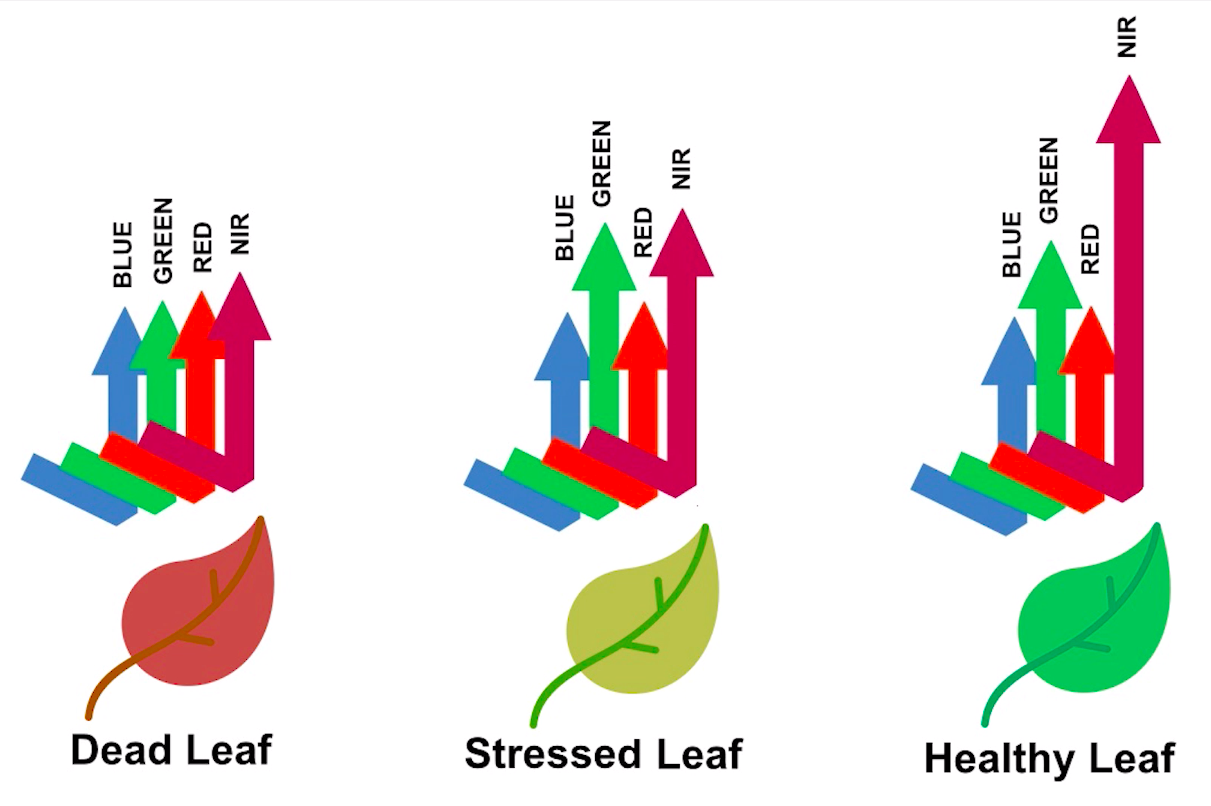
\includegraphics[keepaspectratio]{img/earth-analytics/remote-sensing/spectral_vegetation_stress.png}}
\textgreater{} Image source:
\href{https://github.com/px39n/Awesome-Vegetation-Index}{Spectral
signature literature review by px39n}

Different species of plants reflect different spectral signatures, but
the \emph{pattern} of the signatures across species and sitations is
similar. NDVI compares the amount of NIR reflectance to the amount of
Red reflectance, thus accounting for many of the species differences and
isolating the health of the plant. The formula for calculating NDVI is:

\[NDVI = \frac{(NIR - Red)}{(NIR + Red)}\]

\begin{tcolorbox}[enhanced jigsaw, colbacktitle=quarto-callout-color!10!white, opacityback=0, bottomtitle=1mm, toptitle=1mm, bottomrule=.15mm, left=2mm, colframe=quarto-callout-color-frame, leftrule=.75mm, opacitybacktitle=0.6, colback=white, rightrule=.15mm, toprule=.15mm, breakable, titlerule=0mm, title=\textcolor{quarto-callout-color}{\faInfo}\hspace{0.5em}{Read More}, coltitle=black, arc=.35mm]

Read more about NDVI and other vegetation indices:

\begin{itemize}
\tightlist
\item
  \href{https://www.earthdatascience.org/courses/use-data-open-source-python/multispectral-remote-sensing/vegetation-indices-in-python/calculate-NDVI-python/}{earthdatascience.org}
\item
  \href{https://www.usgs.gov/landsat-missions/landsat-surface-reflectance-derived-spectral-indices}{USGS}
\end{itemize}

\end{tcolorbox}

\bookmarksetup{startatroot}

\chapter{STEP 0: Set up}\label{step-0-set-up}

First, you can use the following parameters to change things about the
workflow:

\begin{Shaded}
\begin{Highlighting}[]
\BuiltInTok{id} \OperatorTok{=} \StringTok{\textquotesingle{}stars\textquotesingle{}}
\NormalTok{site\_name }\OperatorTok{=} \StringTok{\textquotesingle{}Gila River Indian Community\textquotesingle{}}
\NormalTok{project\_name }\OperatorTok{=} \StringTok{\textquotesingle{}Gila River Vegetation\textquotesingle{}}
\NormalTok{boundary\_dir }\OperatorTok{=} \StringTok{\textquotesingle{}tl\_2020\_us\_aitsn\textquotesingle{}}
\NormalTok{event }\OperatorTok{=} \StringTok{\textquotesingle{}water rights case\textquotesingle{}}
\NormalTok{start\_year }\OperatorTok{=} \StringTok{\textquotesingle{}2001\textquotesingle{}}
\NormalTok{end\_year }\OperatorTok{=} \StringTok{\textquotesingle{}2022\textquotesingle{}}
\NormalTok{event\_year }\OperatorTok{=} \StringTok{\textquotesingle{}2012\textquotesingle{}}
\end{Highlighting}
\end{Shaded}

\section{Import libraries}\label{import-libraries}

We'll need some Python libraries to complete this workflow.

\begin{tcolorbox}[enhanced jigsaw, colbacktitle=quarto-callout-color!10!white, opacityback=0, bottomtitle=1mm, toptitle=1mm, bottomrule=.15mm, left=2mm, colframe=quarto-callout-color-frame, leftrule=.75mm, opacitybacktitle=0.6, colback=white, rightrule=.15mm, toprule=.15mm, breakable, titlerule=0mm, title=\textcolor{quarto-callout-color}{\faInfo}\hspace{0.5em}{Try It: Import necessary libraries}, coltitle=black, arc=.35mm]

In the cell below, making sure to keep the packages in order, add
packages for:

\begin{itemize}
\tightlist
\item
  Working with DataFrames
\item
  Working with GeoDataFrames
\item
  Making interactive plots of tabular and vector data
\end{itemize}

\end{tcolorbox}

\begin{tcolorbox}[enhanced jigsaw, colbacktitle=quarto-callout-color!10!white, opacityback=0, bottomtitle=1mm, toptitle=1mm, bottomrule=.15mm, left=2mm, colframe=quarto-callout-color-frame, leftrule=.75mm, opacitybacktitle=0.6, colback=white, rightrule=.15mm, toprule=.15mm, breakable, titlerule=0mm, title=\textcolor{quarto-callout-color}{\faInfo}\hspace{0.5em}{Reflect and Respond}, coltitle=black, arc=.35mm]

What are we using the rest of these packages for? See if you can figure
it out as you complete the notebook.

\end{tcolorbox}

\begin{Shaded}
\begin{Highlighting}[]
\ImportTok{import}\NormalTok{ json}
\ImportTok{from}\NormalTok{ glob }\ImportTok{import}\NormalTok{ glob}

\ImportTok{import}\NormalTok{ earthpy}
\ImportTok{import}\NormalTok{ hvplot.xarray}
\ImportTok{import}\NormalTok{ rioxarray }\ImportTok{as}\NormalTok{ rxr}
\ImportTok{import}\NormalTok{ xarray }\ImportTok{as}\NormalTok{ xr}
\end{Highlighting}
\end{Shaded}

\section{Download sample data}\label{download-sample-data}

In this analysis, you'll need to download multiple data files to your
computer rather than streaming them from the web. You'll need to set up
a folder for the files, and while you're at it download the sample data
there.

\begin{tcolorbox}[enhanced jigsaw, colbacktitle=quarto-callout-caution-color!10!white, opacityback=0, bottomtitle=1mm, toptitle=1mm, bottomrule=.15mm, left=2mm, colframe=quarto-callout-caution-color-frame, leftrule=.75mm, opacitybacktitle=0.6, colback=white, rightrule=.15mm, toprule=.15mm, breakable, titlerule=0mm, title={GOTCHA ALERT!}, coltitle=black, arc=.35mm]

A lot of times in Python we say ``directory'' to mean a ``folder'' on
your computer. The two words mean the same thing in this context.

\end{tcolorbox}

\begin{tcolorbox}[enhanced jigsaw, colbacktitle=quarto-callout-color!10!white, opacityback=0, bottomtitle=1mm, toptitle=1mm, bottomrule=.15mm, left=2mm, colframe=quarto-callout-color-frame, leftrule=.75mm, opacitybacktitle=0.6, colback=white, rightrule=.15mm, toprule=.15mm, breakable, titlerule=0mm, title=\textcolor{quarto-callout-color}{\faInfo}\hspace{0.5em}{Try It}, coltitle=black, arc=.35mm]

In the cell below, replace `Project Name' with
`\textbf{?meta:params.project\_name} and 'my-data-folder' with a
\textbf{descriptive} directory name.

\end{tcolorbox}

\begin{Shaded}
\begin{Highlighting}[]
\NormalTok{project }\OperatorTok{=}\NormalTok{ earthpy.Project(}
    \StringTok{\textquotesingle{}Project Name\textquotesingle{}}\NormalTok{, dirname}\OperatorTok{=}\StringTok{\textquotesingle{}my{-}data{-}folder\textquotesingle{}}\NormalTok{)}
\NormalTok{project.get\_data()}
\end{Highlighting}
\end{Shaded}

If the water rights case took place in 2004, why are we listing the
event year as \textbf{?meta:params.event\_year}? It takes time for
practices to adjust. You can experiment with different years to see if
it affects the results.

\bookmarksetup{startatroot}

\chapter{STEP 1: Site map}\label{step-1-site-map}

\section{\texorpdfstring{Study Area:
\textbf{?meta:params.site\_name}}{Study Area: ?meta:params.site\_name}}\label{study-area}

\begin{tcolorbox}[enhanced jigsaw, colbacktitle=quarto-callout-color!10!white, opacityback=0, bottomtitle=1mm, toptitle=1mm, bottomrule=.15mm, left=2mm, colframe=quarto-callout-color-frame, leftrule=.75mm, opacitybacktitle=0.6, colback=white, rightrule=.15mm, toprule=.15mm, breakable, titlerule=0mm, title=\textcolor{quarto-callout-color}{\faInfo}\hspace{0.5em}{Reflect and Respond}, coltitle=black, arc=.35mm]

For this coding challenge, we are interested in the boundary of the
\textbf{?meta:params.site\_name}, and the health of vegetation in the
area measured on a scale from -1 to 1. In the cell below, answer the
following question: \textbf{What data type do you think the boundary
will be? What about the vegetation health?}

\end{tcolorbox}

\subsection{\texorpdfstring{Load the \textbf{?meta:params.site\_name}
boundary}{Load the ?meta:params.site\_name boundary}}\label{load-the-boundary}

\begin{tcolorbox}[enhanced jigsaw, colbacktitle=quarto-callout-color!10!white, opacityback=0, bottomtitle=1mm, toptitle=1mm, bottomrule=.15mm, left=2mm, colframe=quarto-callout-color-frame, leftrule=.75mm, opacitybacktitle=0.6, colback=white, rightrule=.15mm, toprule=.15mm, breakable, titlerule=0mm, title=\textcolor{quarto-callout-color}{\faInfo}\hspace{0.5em}{Try It}, coltitle=black, arc=.35mm]

\begin{itemize}
\tightlist
\item
  Locate the boundary files in your download directory
\item
  Change \texttt{\textquotesingle{}boundary-directory\textquotesingle{}}
  to the actual location
\item
  Load the data into Python and check that it worked
\end{itemize}

\end{tcolorbox}

\begin{Shaded}
\begin{Highlighting}[]
\CommentTok{\# Load in the boundary data}
\NormalTok{aitsn\_gdf }\OperatorTok{=}\NormalTok{ gpd.read\_file(project.project\_dir }\OperatorTok{/} \StringTok{\textquotesingle{}boundary{-}directory\textquotesingle{}}\NormalTok{)}
\CommentTok{\# Check that it worked}
\end{Highlighting}
\end{Shaded}

You might notice in this dataset that some of the names are not easily
searchable. For example, the Gila River subdivisions are named
``District 1-7''! So, how do we know what to search for? We recommend
making an \textbf{interactive} plot of the data so that you can find the
information you need, e.g.:

\begin{Shaded}
\begin{Highlighting}[]
\NormalTok{aitsn\_gdf.hvplot(}
\NormalTok{    geo}\OperatorTok{=}\VariableTok{True}\NormalTok{, tiles}\OperatorTok{=}\StringTok{\textquotesingle{}EsriImagery\textquotesingle{}}\NormalTok{, }
\NormalTok{    frame\_width}\OperatorTok{=}\DecValTok{500}\NormalTok{,}
\NormalTok{    legend}\OperatorTok{=}\VariableTok{False}\NormalTok{, fill\_color}\OperatorTok{=}\VariableTok{None}\NormalTok{, edge\_color}\OperatorTok{=}\StringTok{\textquotesingle{}white\textquotesingle{}}\NormalTok{,}
    \CommentTok{\# This parameter makes all the column values in the dataset visible.}
\NormalTok{    hover\_cols}\OperatorTok{=}\StringTok{\textquotesingle{}all\textquotesingle{}}\NormalTok{)}
\end{Highlighting}
\end{Shaded}

\begin{verbatim}
WARNING:param.main: edge_color option not found for polygons plot with bokeh; similar options include: ['muted_color', 'bgcolor', 'line_color']
\end{verbatim}

\begin{verbatim}
:Overlay
   .WMTS.I     :WMTS   [Longitude,Latitude]
   .Polygons.I :Polygons   [Longitude,Latitude]   (index,AIANNHCE,TRSUBCE,TRSUBNS,GEOID,NAME,NAMELSAD,LSAD,CLASSFP,MTFCC,FUNCSTAT,ALAND,AWATER,INTPTLAT,INTPTLON)
\end{verbatim}

\begin{tcolorbox}[enhanced jigsaw, colbacktitle=quarto-callout-color!10!white, opacityback=0, bottomtitle=1mm, toptitle=1mm, bottomrule=.15mm, left=2mm, colframe=quarto-callout-color-frame, leftrule=.75mm, opacitybacktitle=0.6, colback=white, rightrule=.15mm, toprule=.15mm, breakable, titlerule=0mm, title=\textcolor{quarto-callout-color}{\faInfo}\hspace{0.5em}{Reflect and Respond}, coltitle=black, arc=.35mm]

What column could you use to uniquely identify the subdivisions of the
reservation you want to study using this interactive map? What value do
you need to use to filter the \texttt{GeoDataFrame}?

\end{tcolorbox}

Now that you have the info you need, it's also a good idea to check the
data type. For example, we suggest looking at the \texttt{AIANNHCE}
column\ldots but is that value some kind of \textbf{number} or an
\textbf{object} like a text string? We can't tell just by looking, which
is where our friend the \texttt{.info()} method comes in:

\begin{Shaded}
\begin{Highlighting}[]
\NormalTok{aitsn\_gdf.info()}
\end{Highlighting}
\end{Shaded}

\begin{verbatim}
<class 'geopandas.geodataframe.GeoDataFrame'>
RangeIndex: 484 entries, 0 to 483
Data columns (total 15 columns):
 #   Column    Non-Null Count  Dtype   
---  ------    --------------  -----   
 0   AIANNHCE  484 non-null    object  
 1   TRSUBCE   484 non-null    object  
 2   TRSUBNS   484 non-null    object  
 3   GEOID     484 non-null    object  
 4   NAME      484 non-null    object  
 5   NAMELSAD  484 non-null    object  
 6   LSAD      484 non-null    object  
 7   CLASSFP   484 non-null    object  
 8   MTFCC     484 non-null    object  
 9   FUNCSTAT  484 non-null    object  
 10  ALAND     484 non-null    int64   
 11  AWATER    484 non-null    int64   
 12  INTPTLAT  484 non-null    object  
 13  INTPTLON  484 non-null    object  
 14  geometry  484 non-null    geometry
dtypes: geometry(1), int64(2), object(12)
memory usage: 56.8+ KB
\end{verbatim}

\begin{tcolorbox}[enhanced jigsaw, colbacktitle=quarto-callout-color!10!white, opacityback=0, bottomtitle=1mm, toptitle=1mm, bottomrule=.15mm, left=2mm, colframe=quarto-callout-color-frame, leftrule=.75mm, opacitybacktitle=0.6, colback=white, rightrule=.15mm, toprule=.15mm, breakable, titlerule=0mm, title=\textcolor{quarto-callout-color}{\faInfo}\hspace{0.5em}{Reflect and Respond}, coltitle=black, arc=.35mm]

What is the data type of the \texttt{AIANNHCE} column? How will that
affect your code?

\end{tcolorbox}

Let's go ahead and select the Gila River subdivisions, and make a site
map.

\begin{tcolorbox}[enhanced jigsaw, colbacktitle=quarto-callout-color!10!white, opacityback=0, bottomtitle=1mm, toptitle=1mm, bottomrule=.15mm, left=2mm, colframe=quarto-callout-color-frame, leftrule=.75mm, opacitybacktitle=0.6, colback=white, rightrule=.15mm, toprule=.15mm, breakable, titlerule=0mm, title=\textcolor{quarto-callout-color}{\faInfo}\hspace{0.5em}{Try It}, coltitle=black, arc=.35mm]

\begin{enumerate}
\def\labelenumi{\arabic{enumi}.}
\tightlist
\item
  Replace \texttt{identifier} with the value you found from exploring
  the interactive map. Make sure that you are using the correct
  \textbf{data type}!
\item
  Change the plot to have a web tile basemap, and look the way you want
  it to.
\end{enumerate}

\end{tcolorbox}

\begin{Shaded}
\begin{Highlighting}[]
\CommentTok{\# Select and merge the subdivisions you want}
\NormalTok{gdf }\OperatorTok{=}\NormalTok{ aitsn\_gdf.loc[aitsn\_gdf.AIANNHCE}\OperatorTok{==}\NormalTok{identifier].dissolve()}
\CommentTok{\# Plot the results with web tile images}
\NormalTok{gdf.hvplot()}
\end{Highlighting}
\end{Shaded}

\bookmarksetup{startatroot}

\chapter{STEP 2: Wrangle Raster Data}\label{step-2-wrangle-raster-data}

\section{Load in NDVI data}\label{load-in-ndvi-data}

Now you need to load all the downloaded files into Python. Let's start
by getting all the file names. You will also need to extract the date
from the filename. Check out
\href{https://www.earthdatascience.org/courses/intro-to-earth-data-science/write-efficient-python-code/loops/data-workflows-with-loops/}{the
lesson on getting information from filenames in the textbook}.

Instead of writing out the names of all the files you want, you can use
the \texttt{glob} utility to find all files that match a
\textbf{pattern} formed with the \textbf{wildcard} character \texttt{*}.
The wildcard can represent any string of alphanumeric characters. For
example, the pattern
\texttt{\textquotesingle{}file\_*.tif\textquotesingle{}} will match the
files \texttt{\textquotesingle{}file\_1.tif\textquotesingle{}},
\texttt{\textquotesingle{}file\_2.tiv\textquotesingle{}}, or even
\texttt{\textquotesingle{}file\_qeoiurghtfoqaegbn34pf.tif\textquotesingle{}}\ldots{}
but it will not match
\texttt{\textquotesingle{}something-else.csv\textquotesingle{}} or even
\texttt{\textquotesingle{}something-else.tif\textquotesingle{}}.

In this notebook, we'll use the \texttt{.rglob()}, or \textbf{recursive}
glob method of the Path object instead. It works similarly, but you'll
notice that we have to convert the results to a list with the
\texttt{list()} function.

\begin{tcolorbox}[enhanced jigsaw, colbacktitle=quarto-callout-caution-color!10!white, opacityback=0, bottomtitle=1mm, toptitle=1mm, bottomrule=.15mm, left=2mm, colframe=quarto-callout-caution-color-frame, leftrule=.75mm, opacitybacktitle=0.6, colback=white, rightrule=.15mm, toprule=.15mm, breakable, titlerule=0mm, title=\textcolor{quarto-callout-caution-color}{\faFire}\hspace{0.5em}{GOTCHA ALERT!}, coltitle=black, arc=.35mm]

\texttt{glob} doesn't necessarily find files in the order you would
expect. Make sure to \textbf{sort} your file names like it says in the
textbook.

\end{tcolorbox}

\begin{tcolorbox}[enhanced jigsaw, colbacktitle=quarto-callout-color!10!white, opacityback=0, bottomtitle=1mm, toptitle=1mm, bottomrule=.15mm, left=2mm, colframe=quarto-callout-color-frame, leftrule=.75mm, opacitybacktitle=0.6, colback=white, rightrule=.15mm, toprule=.15mm, breakable, titlerule=0mm, title=\textcolor{quarto-callout-color}{\faInfo}\hspace{0.5em}{Reflect and Respond}, coltitle=black, arc=.35mm]

Take a look at the file names for the NDVI files. What do you notice is
the same for all the files? Keep in mind that for this analysis you only
want to import the NDVI files, not the Quality files (which would be
used to identify potential incorrect measurements).

\end{tcolorbox}

\begin{tcolorbox}[enhanced jigsaw, colbacktitle=quarto-callout-color!10!white, opacityback=0, bottomtitle=1mm, toptitle=1mm, bottomrule=.15mm, left=2mm, colframe=quarto-callout-color-frame, leftrule=.75mm, opacitybacktitle=0.6, colback=white, rightrule=.15mm, toprule=.15mm, breakable, titlerule=0mm, title=\textcolor{quarto-callout-color}{\faInfo}\hspace{0.5em}{Try It}, coltitle=black, arc=.35mm]

\begin{enumerate}
\def\labelenumi{\arabic{enumi}.}
\tightlist
\item
  Create a \textbf{pattern} for the files you want to import. Your
  pattern should include the parts of the file names that are the same
  for all files, and replace the rest with the \texttt{*} character.
  Make sure to match the NDVI files, but not the Quality files!
\item
  Replace \texttt{ndvi-pattern} with your pattern
\item
  Run the code and make sure that you are getting all the files you want
  and none of the files you don't!
\end{enumerate}

\end{tcolorbox}

\begin{Shaded}
\begin{Highlighting}[]
\CommentTok{\# Get a sorted list of NDVI tif file paths}
\NormalTok{ndvi\_paths }\OperatorTok{=} \BuiltInTok{sorted}\NormalTok{(}\BuiltInTok{list}\NormalTok{(project.project\_dir.rglob(}\StringTok{\textquotesingle{}ndvi{-}pattern\textquotesingle{}}\NormalTok{)))}

\CommentTok{\# Display the first and last three files paths to check the pattern}
\NormalTok{ndvi\_paths[:}\DecValTok{3}\NormalTok{], ndvi\_paths[}\OperatorTok{{-}}\DecValTok{3}\NormalTok{:]}
\end{Highlighting}
\end{Shaded}

\section{Repeating tasks in Python}\label{repeating-tasks-in-python}

Now you should have a few dozen files! For each file, you need to:

\begin{itemize}
\tightlist
\item
  Load the file in using the \texttt{rioxarray} library
\item
  Get the date from the file name
\item
  Add the date as a dimension coordinate
\item
  Give your data variable a name
\end{itemize}

You don't want to write out the code for each file! That's a recipe for
copy pasta. Luckily, Python has tools for doing similar tasks
repeatedly. In this case, you'll use one called a \texttt{for} loop.

There's some code below that uses a \texttt{for} loop in what is called
an \textbf{accumulation pattern} to process each file. That means that
you will save the results of your processing to a list each time you
process the files, and then merge all the arrays in the list.

\begin{tcolorbox}[enhanced jigsaw, colbacktitle=quarto-callout-color!10!white, opacityback=0, bottomtitle=1mm, toptitle=1mm, bottomrule=.15mm, left=2mm, colframe=quarto-callout-color-frame, leftrule=.75mm, opacitybacktitle=0.6, colback=white, rightrule=.15mm, toprule=.15mm, breakable, titlerule=0mm, title=\textcolor{quarto-callout-color}{\faInfo}\hspace{0.5em}{Try It}, coltitle=black, arc=.35mm]

\begin{itemize}
\tightlist
\item
  Look at the file names. How many characters from the end is the date?
  \texttt{doy\_start} and \texttt{doy\_end} are used to extract the day
  of the year (doy) from the file name. You will need to count
  characters from the end and change the values to get the right part of
  the file name. HINT: the index -1 in Python means the last value, -2
  second-to-last, and so on.
\item
  Replace any required variable names with your chosen variable names
\end{itemize}

\end{tcolorbox}

\begin{Shaded}
\begin{Highlighting}[]
\NormalTok{doy\_start }\OperatorTok{=} \OperatorTok{{-}}\DecValTok{1}
\NormalTok{doy\_end }\OperatorTok{=} \OperatorTok{{-}}\DecValTok{1}

\CommentTok{\# Loop through each NDVI image}
\NormalTok{ndvi\_das }\OperatorTok{=}\NormalTok{ []}
\ControlFlowTok{for}\NormalTok{ ndvi\_path }\KeywordTok{in}\NormalTok{ ndvi\_paths:}
    \CommentTok{\# Get date from file name}

    \CommentTok{\# Open dataset}

    \CommentTok{\# Add date dimension and clean up metadata}
\NormalTok{    da }\OperatorTok{=}\NormalTok{ da.assign\_coords(\{}\StringTok{\textquotesingle{}date\textquotesingle{}}\NormalTok{: date\})}
\NormalTok{    da }\OperatorTok{=}\NormalTok{ da.expand\_dims(\{}\StringTok{\textquotesingle{}date\textquotesingle{}}\NormalTok{: }\DecValTok{1}\NormalTok{\})}
\NormalTok{    da.name }\OperatorTok{=} \StringTok{\textquotesingle{}NDVI\textquotesingle{}}

    \CommentTok{\# Prepare for concatenation}
\end{Highlighting}
\end{Shaded}

\section{Combine Rasters}\label{combine-rasters}

Next, stack your arrays by date into a time series using the
\texttt{xr.combine\_by\_coords()} function. You will have to tell it
which dimension you want to stack your data in.

\begin{Shaded}
\begin{Highlighting}[]
\CommentTok{\# Combine NDVI images from all dates}
\end{Highlighting}
\end{Shaded}

\bookmarksetup{startatroot}

\chapter{STEP 3: Plot NDVI}\label{step-3-plot-ndvi}

\begin{tcolorbox}[enhanced jigsaw, colbacktitle=quarto-callout-color!10!white, opacityback=0, bottomtitle=1mm, toptitle=1mm, bottomrule=.15mm, left=2mm, colframe=quarto-callout-color-frame, leftrule=.75mm, opacitybacktitle=0.6, colback=white, rightrule=.15mm, toprule=.15mm, breakable, titlerule=0mm, title=\textcolor{quarto-callout-color}{\faInfo}\hspace{0.5em}{Try It: Plot the change in NDVI spatially}, coltitle=black, arc=.35mm]

Complete the following:

\begin{itemize}
\tightlist
\item
  Select data from before the \textbf{?meta:params.event}
  (\textbf{?meta:params.start\_year} to
  \textbf{?meta:params.event\_year})
\item
  Take the temporal mean (over the \textbf{date}, not spatially)
\item
  Get the NDVI variable (should be a DataArray, not a Dataset)
\item
  Repeat for the data from after the \textbf{?meta:params.event}
  (\textbf{?meta:params.event\_year} to \textbf{?meta:params.end\_year})
\item
  Subtract the pre-event data \textbf{from} the post-event data
\item
  Plot the result using a \textbf{diverging} color map like
  \texttt{cmap=plt.cm.PiYG}
\end{itemize}

There are different types of color maps for different types of data. In
this case, we want decreases to be a different color from increases, so
we should use a \textbf{diverging} color map. Check out available
colormaps in the
\href{https://matplotlib.org/stable/tutorials/colors/colormaps.html}{matplotlib
documentation}.

\end{tcolorbox}

\begin{tcolorbox}[enhanced jigsaw, colbacktitle=quarto-callout-color!10!white, opacityback=0, bottomtitle=1mm, toptitle=1mm, bottomrule=.15mm, left=2mm, colframe=quarto-callout-color-frame, leftrule=.75mm, opacitybacktitle=0.6, colback=white, rightrule=.15mm, toprule=.15mm, breakable, titlerule=0mm, title=\textcolor{quarto-callout-color}{\faInfo}\hspace{0.5em}{Looking for an Extra Challenge?}, coltitle=black, arc=.35mm]

For an extra challenge, add the \textbf{?meta:params.site\_name}
boundary to the plot.

\end{tcolorbox}

\begin{Shaded}
\begin{Highlighting}[]
\CommentTok{\# Compute the difference in NDVI before and after}

\CommentTok{\# Plot the difference}
\NormalTok{(}
\NormalTok{    ndvi\_diff.hvplot(x}\OperatorTok{=}\StringTok{\textquotesingle{}\textquotesingle{}}\NormalTok{, y}\OperatorTok{=}\StringTok{\textquotesingle{}\textquotesingle{}}\NormalTok{, cmap}\OperatorTok{=}\StringTok{\textquotesingle{}\textquotesingle{}}\NormalTok{, geo}\OperatorTok{=}\VariableTok{True}\NormalTok{)}
    \OperatorTok{*}
\NormalTok{    gdf.hvplot(geo}\OperatorTok{=}\VariableTok{True}\NormalTok{, fill\_color}\OperatorTok{=}\VariableTok{None}\NormalTok{, line\_color}\OperatorTok{=}\StringTok{\textquotesingle{}black\textquotesingle{}}\NormalTok{)}
\NormalTok{)}
\end{Highlighting}
\end{Shaded}

\bookmarksetup{startatroot}

\chapter{\texorpdfstring{STEP 4: Is the NDVI different within the
\textbf{?meta:params.site\_name} after the
\textbf{?meta:params.event}?}{STEP 4: Is the NDVI different within the ?meta:params.site\_name after the ?meta:params.event?}}\label{step-4-is-the-ndvi-different-within-the-after-the}

You will compute the mean NDVI inside and outside the fire boundary.
First, use the code below to get a \texttt{GeoDataFrame} of the area
outside the Reservation.

\begin{tcolorbox}[enhanced jigsaw, colbacktitle=quarto-callout-color!10!white, opacityback=0, bottomtitle=1mm, toptitle=1mm, bottomrule=.15mm, left=2mm, colframe=quarto-callout-color-frame, leftrule=.75mm, opacitybacktitle=0.6, colback=white, rightrule=.15mm, toprule=.15mm, breakable, titlerule=0mm, title=\textcolor{quarto-callout-color}{\faInfo}\hspace{0.5em}{Try It}, coltitle=black, arc=.35mm]

\begin{enumerate}
\def\labelenumi{\arabic{enumi}.}
\tightlist
\item
  Check the variable names - Make sure that the code uses your boundary
  \texttt{GeoDataFrame}
\item
  How could you test if the geometry was modified correctly? Add some
  code to take a look at the results.
\end{enumerate}

\end{tcolorbox}

\begin{Shaded}
\begin{Highlighting}[]
\CommentTok{\# Compute the area outside the fire boundary}
\end{Highlighting}
\end{Shaded}

Next, clip your DataArray to the boundaries for both inside and outside
the reservation. You will need to replace the \texttt{GeoDataFrame} name
with your own. Check out the
\href{https://www.earthdatascience.org/courses/use-data-open-source-python/intro-raster-data-python/raster-data-processing/crop-raster-data-with-shapefile-in-python/}{lesson
on clipping data with the \texttt{rioxarray} library in the textbook}.

\begin{tcolorbox}[enhanced jigsaw, colbacktitle=quarto-callout-caution-color!10!white, opacityback=0, bottomtitle=1mm, toptitle=1mm, bottomrule=.15mm, left=2mm, colframe=quarto-callout-caution-color-frame, leftrule=.75mm, opacitybacktitle=0.6, colback=white, rightrule=.15mm, toprule=.15mm, breakable, titlerule=0mm, title=\textcolor{quarto-callout-caution-color}{\faFire}\hspace{0.5em}{GOTCHA ALERT}, coltitle=black, arc=.35mm]

It's important to use \texttt{from\_disk=True} when clipping large
arrays like this. It allows the computer to use less valuable memory
resources when clipping - you will probably find that otherwise the cell
below crashes your kernel.

\end{tcolorbox}

\begin{Shaded}
\begin{Highlighting}[]
\CommentTok{\# Clip data to both inside and outside the boundary}
\end{Highlighting}
\end{Shaded}

\begin{tcolorbox}[enhanced jigsaw, colbacktitle=quarto-callout-color!10!white, opacityback=0, bottomtitle=1mm, toptitle=1mm, bottomrule=.15mm, left=2mm, colframe=quarto-callout-color-frame, leftrule=.75mm, opacitybacktitle=0.6, colback=white, rightrule=.15mm, toprule=.15mm, breakable, titlerule=0mm, title=\textcolor{quarto-callout-color}{\faInfo}\hspace{0.5em}{Try It}, coltitle=black, arc=.35mm]

For \textbf{both inside and outside} the
\textbf{?meta:params.site\_name} boundary:

\begin{itemize}
\tightlist
\item
  Group the data by year
\item
  Take the mean. You always need to tell reducing methods in
  \texttt{xarray} what dimensions you want to reduce. When you want to
  summarize data across \textbf{all} dimensions, you can use the
  \texttt{...} syntax, e.g.~\texttt{.mean(...)} as a shorthand.
\item
  Select the NDVI variable
\item
  Convert to a DataFrame using the \texttt{to\_dataframe()} method
\item
  Join the two DataFrames for plotting using the \texttt{.join()}
  method. You will need to rename the columns using the
  \texttt{lsuffix=} and \texttt{rsuffix=} parameters
\end{itemize}

Finally, plot annual July means for both inside and outside the
Reservation on the same plot.

\end{tcolorbox}

\begin{tcolorbox}[enhanced jigsaw, colbacktitle=quarto-callout-caution-color!10!white, opacityback=0, bottomtitle=1mm, toptitle=1mm, bottomrule=.15mm, left=2mm, colframe=quarto-callout-caution-color-frame, leftrule=.75mm, opacitybacktitle=0.6, colback=white, rightrule=.15mm, toprule=.15mm, breakable, titlerule=0mm, title=\textcolor{quarto-callout-caution-color}{\faFire}\hspace{0.5em}{GOTCHA ALERT}, coltitle=black, arc=.35mm]

The DateIndex in pandas is a little different from the Datetime
Dimension in xarray. You will need to use the \texttt{.dt.year} syntax
to access information about the year, not just \texttt{.year}.

\end{tcolorbox}

\begin{Shaded}
\begin{Highlighting}[]
\CommentTok{\# Compute mean annual July NDVI}
\end{Highlighting}
\end{Shaded}

Now, take the difference between outside and inside the site boundary
and plot that. What do you observe? Don't forget to write a headline and
description of your plot!

\begin{Shaded}
\begin{Highlighting}[]
\CommentTok{\# Plot difference inside and outside the boundary}
\end{Highlighting}
\end{Shaded}

\bookmarksetup{startatroot}

\chapter{Vegetation Data Access}\label{vegetation-data-access}

Accessing NDVI data on Tribal Subdivisions

\hfill\break

\bookmarksetup{startatroot}

\chapter{STEP 0: Set up}\label{step-0-set-up-1}

\section{Import libraries}\label{import-libraries-1}

We'll need some Python libraries to complete this workflow.

\begin{tcolorbox}[enhanced jigsaw, colbacktitle=quarto-callout-color!10!white, opacityback=0, bottomtitle=1mm, toptitle=1mm, bottomrule=.15mm, left=2mm, colframe=quarto-callout-color-frame, leftrule=.75mm, opacitybacktitle=0.6, colback=white, rightrule=.15mm, toprule=.15mm, breakable, titlerule=0mm, title=\textcolor{quarto-callout-color}{\faInfo}\hspace{0.5em}{Try It: Import necessary libraries}, coltitle=black, arc=.35mm]

In the cell below, making sure to keep the packages in order, add
packages for:

\begin{itemize}
\tightlist
\item
  Working with DataFrames
\item
  Working with GeoDataFrames
\item
  Making interactive plots of tabular and vector data
\end{itemize}

\end{tcolorbox}

\begin{tcolorbox}[enhanced jigsaw, colbacktitle=quarto-callout-color!10!white, opacityback=0, bottomtitle=1mm, toptitle=1mm, bottomrule=.15mm, left=2mm, colframe=quarto-callout-color-frame, leftrule=.75mm, opacitybacktitle=0.6, colback=white, rightrule=.15mm, toprule=.15mm, breakable, titlerule=0mm, title=\textcolor{quarto-callout-color}{\faInfo}\hspace{0.5em}{Reflect and Respond}, coltitle=black, arc=.35mm]

What are we using the rest of these packages for? See if you can figure
it out as you complete the notebook.

\end{tcolorbox}

\begin{Shaded}
\begin{Highlighting}[]
\ImportTok{import}\NormalTok{ json}
\ImportTok{import}\NormalTok{ os}
\ImportTok{import}\NormalTok{ pathlib}
\ImportTok{from}\NormalTok{ glob }\ImportTok{import}\NormalTok{ glob}

\ImportTok{import}\NormalTok{ earthpy.api.appeears }\ImportTok{as}\NormalTok{ eaapp}
\ImportTok{import}\NormalTok{ earthpy}
\ImportTok{import}\NormalTok{ hvplot.xarray}
\ImportTok{import}\NormalTok{ rioxarray }\ImportTok{as}\NormalTok{ rxr}
\ImportTok{import}\NormalTok{ xarray }\ImportTok{as}\NormalTok{ xr}
\end{Highlighting}
\end{Shaded}

Next, we'll set some parameters. You can use these to customize your
workflow.

\begin{Shaded}
\begin{Highlighting}[]
\BuiltInTok{id} \OperatorTok{=} \StringTok{\textquotesingle{}stars\textquotesingle{}}
\NormalTok{site\_name }\OperatorTok{=} \StringTok{\textquotesingle{}Gila River Indian Community\textquotesingle{}}
\NormalTok{data\_dir }\OperatorTok{=} \StringTok{\textquotesingle{}gila{-}river\textquotesingle{}}
\NormalTok{download\_key }\OperatorTok{=} \StringTok{\textquotesingle{}gila{-}river{-}ndvi\textquotesingle{}}
\NormalTok{project\_title }\OperatorTok{=} \StringTok{\textquotesingle{}Gila River Vegetation\textquotesingle{}}
\NormalTok{start\_year }\OperatorTok{=} \DecValTok{2001}
\NormalTok{end\_year }\OperatorTok{=} \DecValTok{2022}
\NormalTok{event\_year }\OperatorTok{=} \DecValTok{2012}
\end{Highlighting}
\end{Shaded}

We have one more setup task. We're not going to be able to load all our
data directly from the web to Python this time. That means we need to
set up a place for it.

\begin{tcolorbox}[enhanced jigsaw, colbacktitle=quarto-callout-caution-color!10!white, opacityback=0, bottomtitle=1mm, toptitle=1mm, bottomrule=.15mm, left=2mm, colframe=quarto-callout-caution-color-frame, leftrule=.75mm, opacitybacktitle=0.6, colback=white, rightrule=.15mm, toprule=.15mm, breakable, titlerule=0mm, title={GOTCHA ALERT!}, coltitle=black, arc=.35mm]

A lot of times in Python we say ``directory'' to mean a ``folder'' on
your computer. The two words mean the same thing in this context.

\end{tcolorbox}

\begin{tcolorbox}[enhanced jigsaw, colbacktitle=quarto-callout-color!10!white, opacityback=0, bottomtitle=1mm, toptitle=1mm, bottomrule=.15mm, left=2mm, colframe=quarto-callout-color-frame, leftrule=.75mm, opacitybacktitle=0.6, colback=white, rightrule=.15mm, toprule=.15mm, breakable, titlerule=0mm, title=\textcolor{quarto-callout-color}{\faInfo}\hspace{0.5em}{Try It}, coltitle=black, arc=.35mm]

\begin{enumerate}
\def\labelenumi{\arabic{enumi}.}
\tightlist
\item
  Replace `my-data-folder' with a \textbf{descriptive} directory name.
\item
  Run the cell to display your project directory.
\item
  Can you find the directory, either in a terminal or through your
  operating system's file browser/explorer/finder?
\end{enumerate}

\end{tcolorbox}

\begin{Shaded}
\begin{Highlighting}[]
\CommentTok{\# Create a project directory in the system data folder}
\NormalTok{project }\OperatorTok{=}\NormalTok{ earthpy.project.Project(dirname}\OperatorTok{=}\StringTok{\textquotesingle{}my{-}data{-}folder\textquotesingle{}}\NormalTok{)}
\NormalTok{project.project\_dir}
\end{Highlighting}
\end{Shaded}

\bookmarksetup{startatroot}

\chapter{STEP 1: Study area}\label{step-1-study-area}

You can use any boundary for your study. In the example, we used the
``American Indian Tribal Subdivisions'' available from the US Census.

\marginnote{\begin{footnotesize}

We realize not everyone is cool with the term ``American Indian'',
especially when used by people who aren't Tribal members. At the same
time, others feel that it is important to reclaim ``Indian'', and more
importantly that's the term a lot of Tribal people use every day. In
this case, we're stuck because of how this dataset is named in the
Census boundary datasets\ldots however, when sharing your work or
publishing your own data, it's important to include local communities in
the area you are studying, about language choices but also
\emph{throughout} your project.

\end{footnotesize}}

We'll be downloading the boundaries using a web browser. The data
source, \href{https://catalog.data.gov/}{data.gov}, has placed
restrictions on programmatic downloads (downloads using code). There are
a number of ways to attempt to get around these restrictions, such as
pretending to be a web browser by setting the \textbf{User Agent}
parameter, but in this case we've found it's just not worth the time and
effort. Follow the steps below to download the data and put it somewhere
that your Python code can find it.

\section{STEP 1A: Open up the data
catalog}\label{step-1a-open-up-the-data-catalog}

Click this link:
\href{https://catalog.data.gov/}{https://catalog.data.gov}. You can also
open your web browser and type it in if you prefer.

\begin{figure}[H]

{\centering \pandocbounded{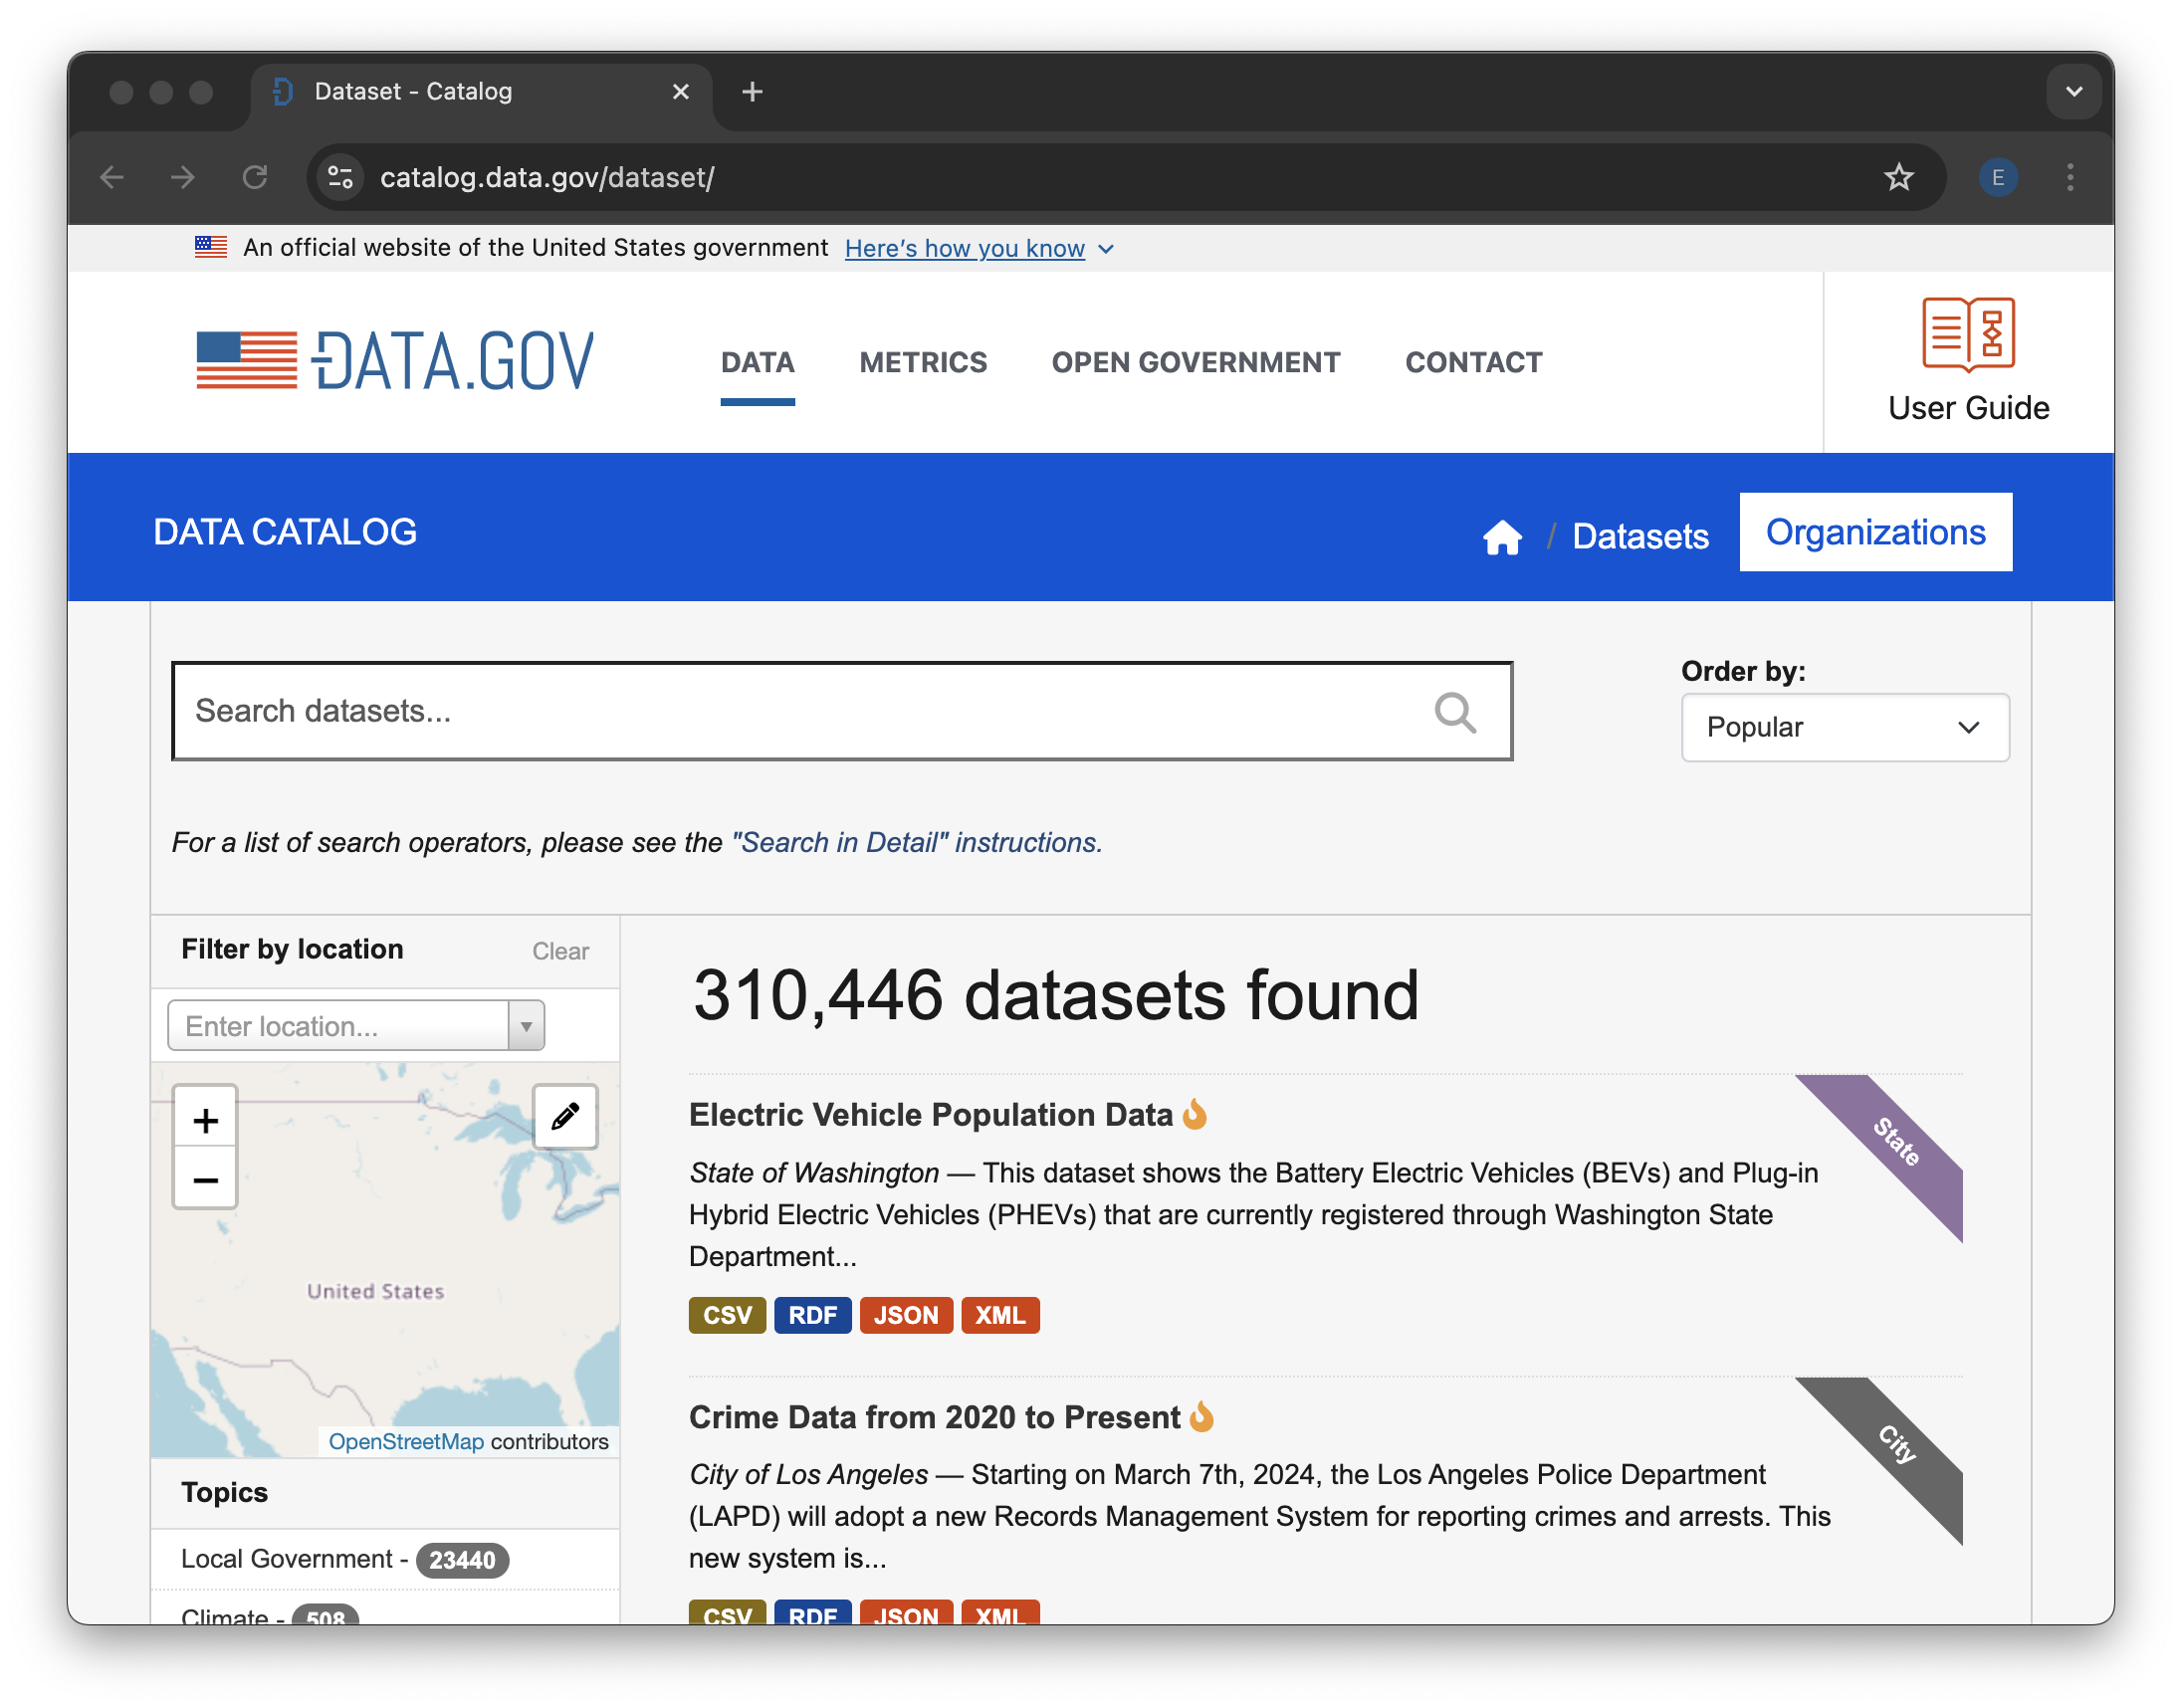
\includegraphics[keepaspectratio]{img/earth-analytics/download/aitsn/01-catalog.png}}

}

\caption{Open up the data.gov catalog.}

\end{figure}%

\section{STEP 1B: Search}\label{step-1b-search}

Search for the data you want. To get the American Indian Tribal
Subdivisions census data, we recommend the search term ``American Indian
Tribal Subdivisions 2020''. These census files are updated regularly at
the time of the census, so we want to make sure we have the most recent
version. The last census was in 2020.

\begin{figure}[H]

{\centering \pandocbounded{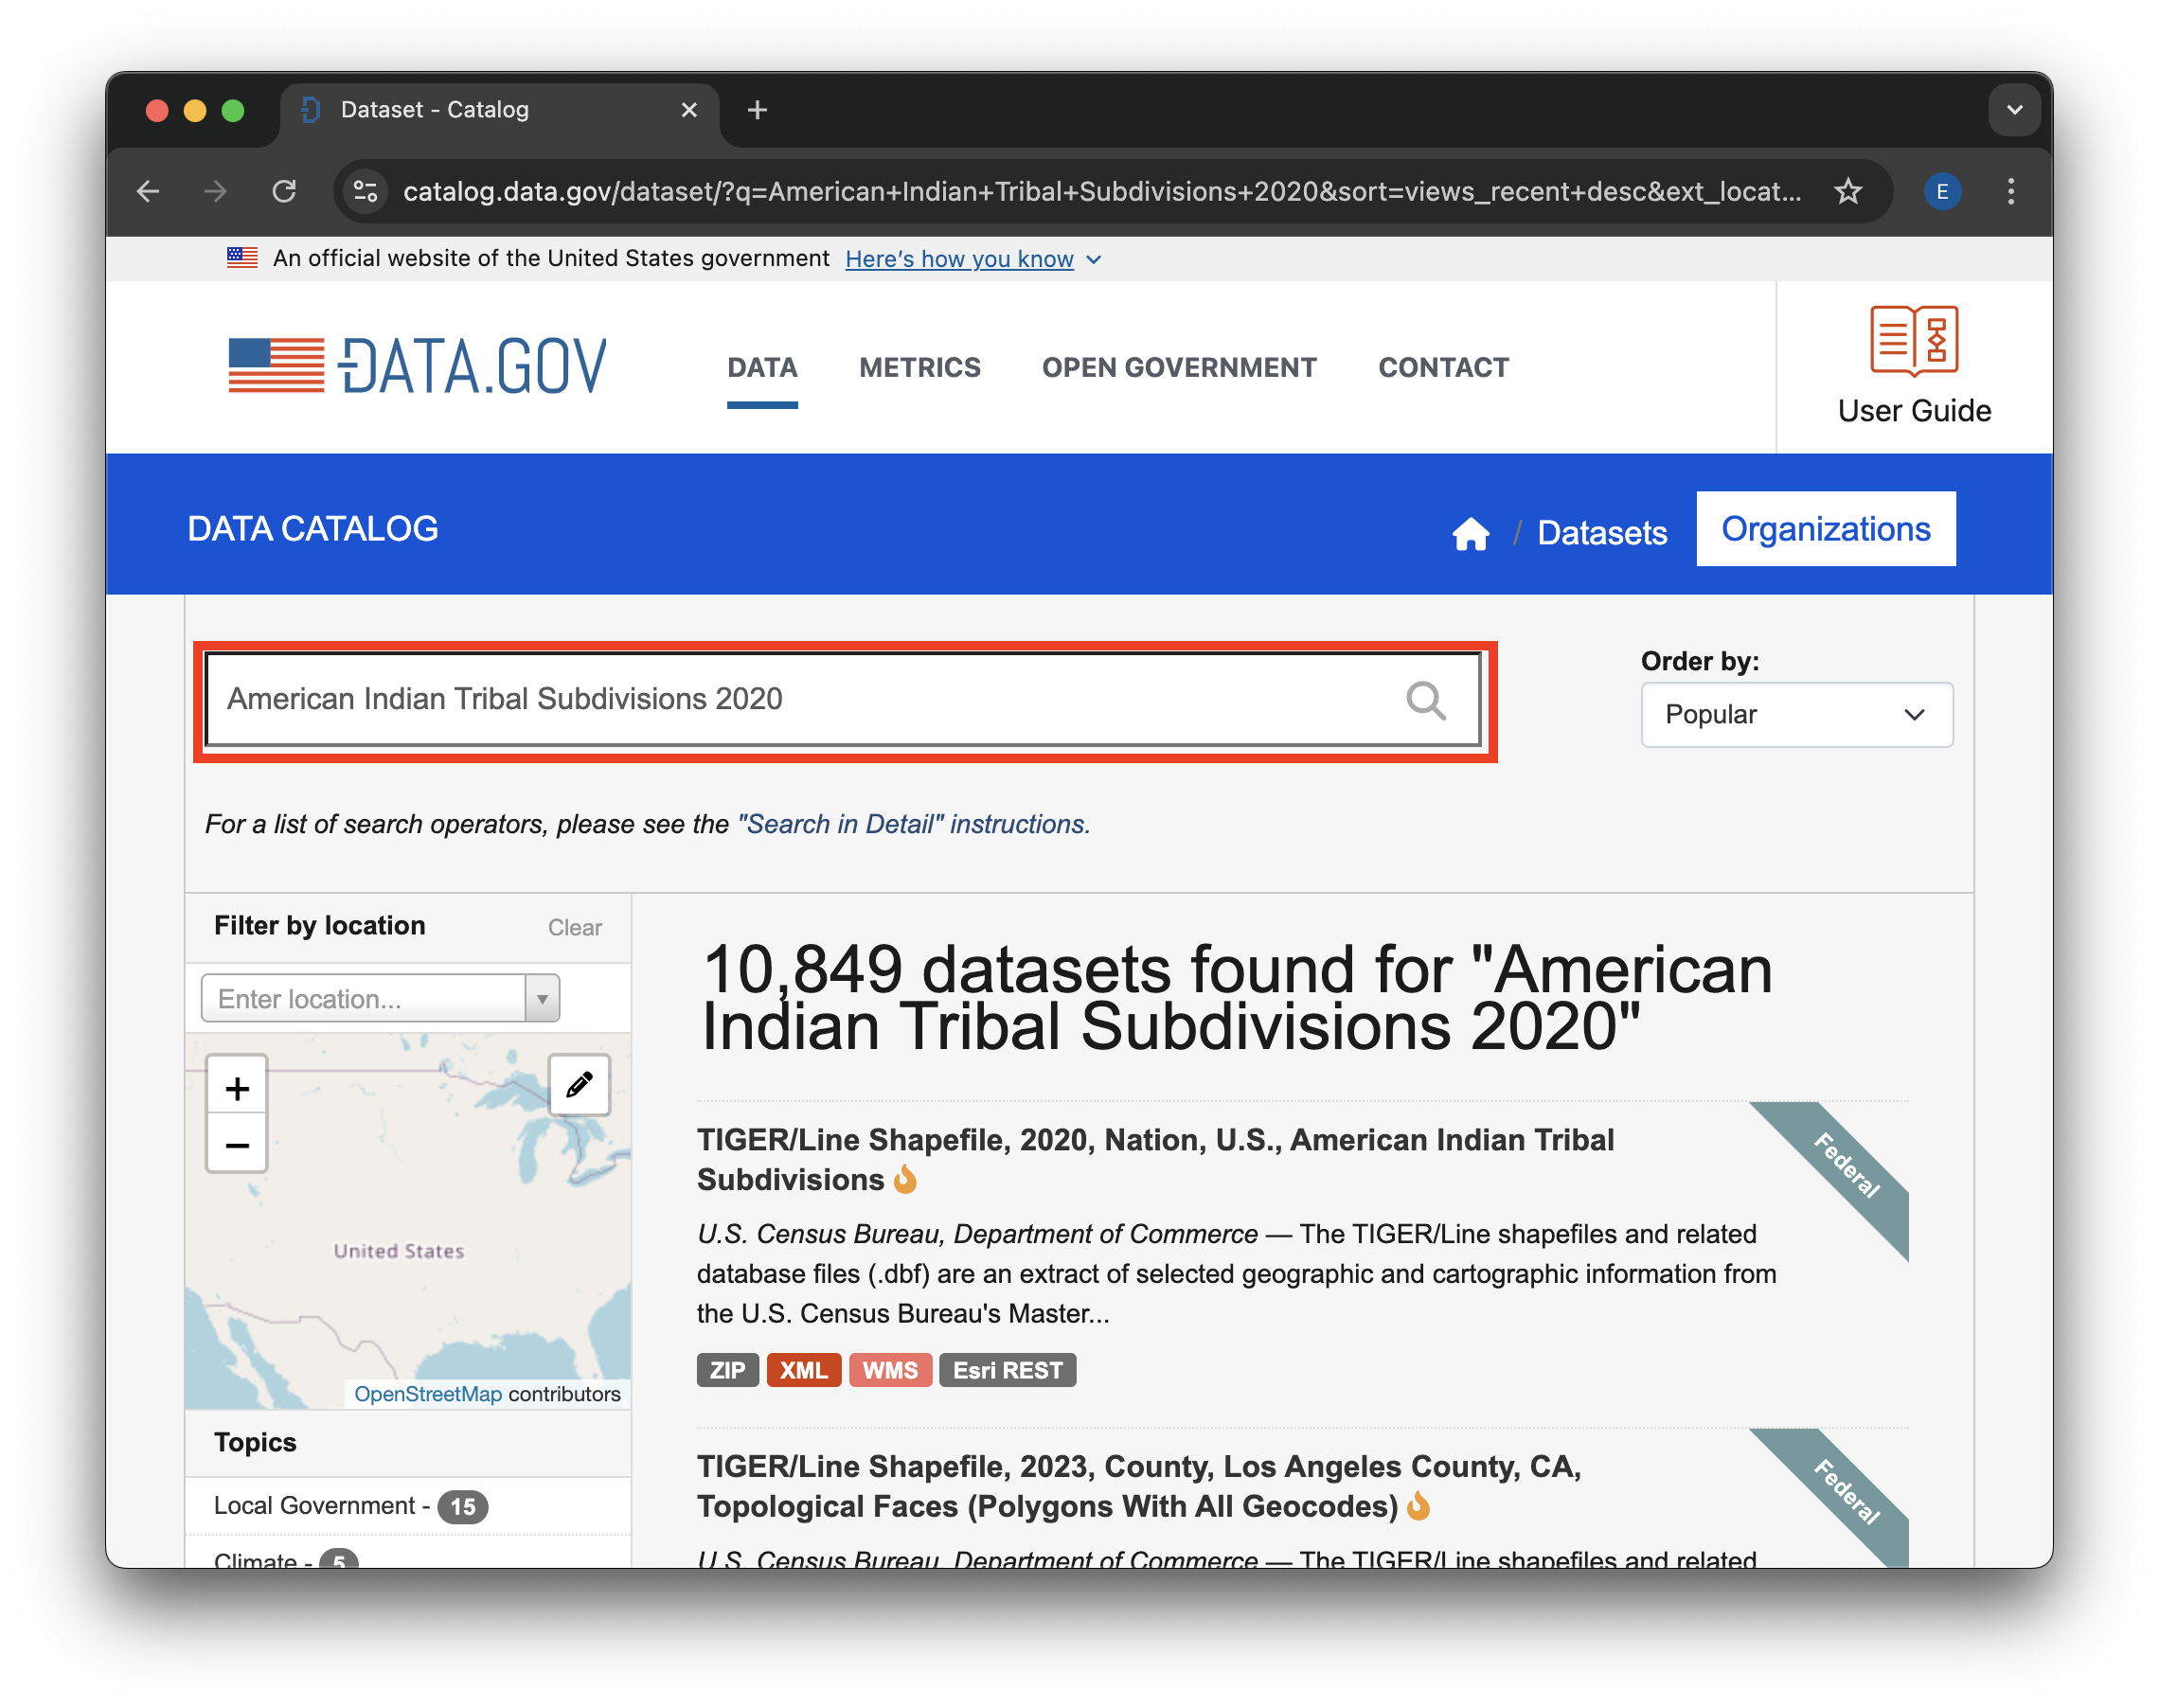
\includegraphics[keepaspectratio]{img/earth-analytics/download/aitsn/02-search.png}}

}

\caption{\textbf{Search} for ``American Indian Tribal Subdivisions
2020''}

\end{figure}%

\section{STEP 1C: Open the dataset
page}\label{step-1c-open-the-dataset-page}

Find the ``TIGER/Line Shapefile, 2020, Nation, U.S., American Indian
Tribal Subdivisions'' dataset in the search results, and click on the
title to go to the dataset page.

\begin{figure}[H]

{\centering \pandocbounded{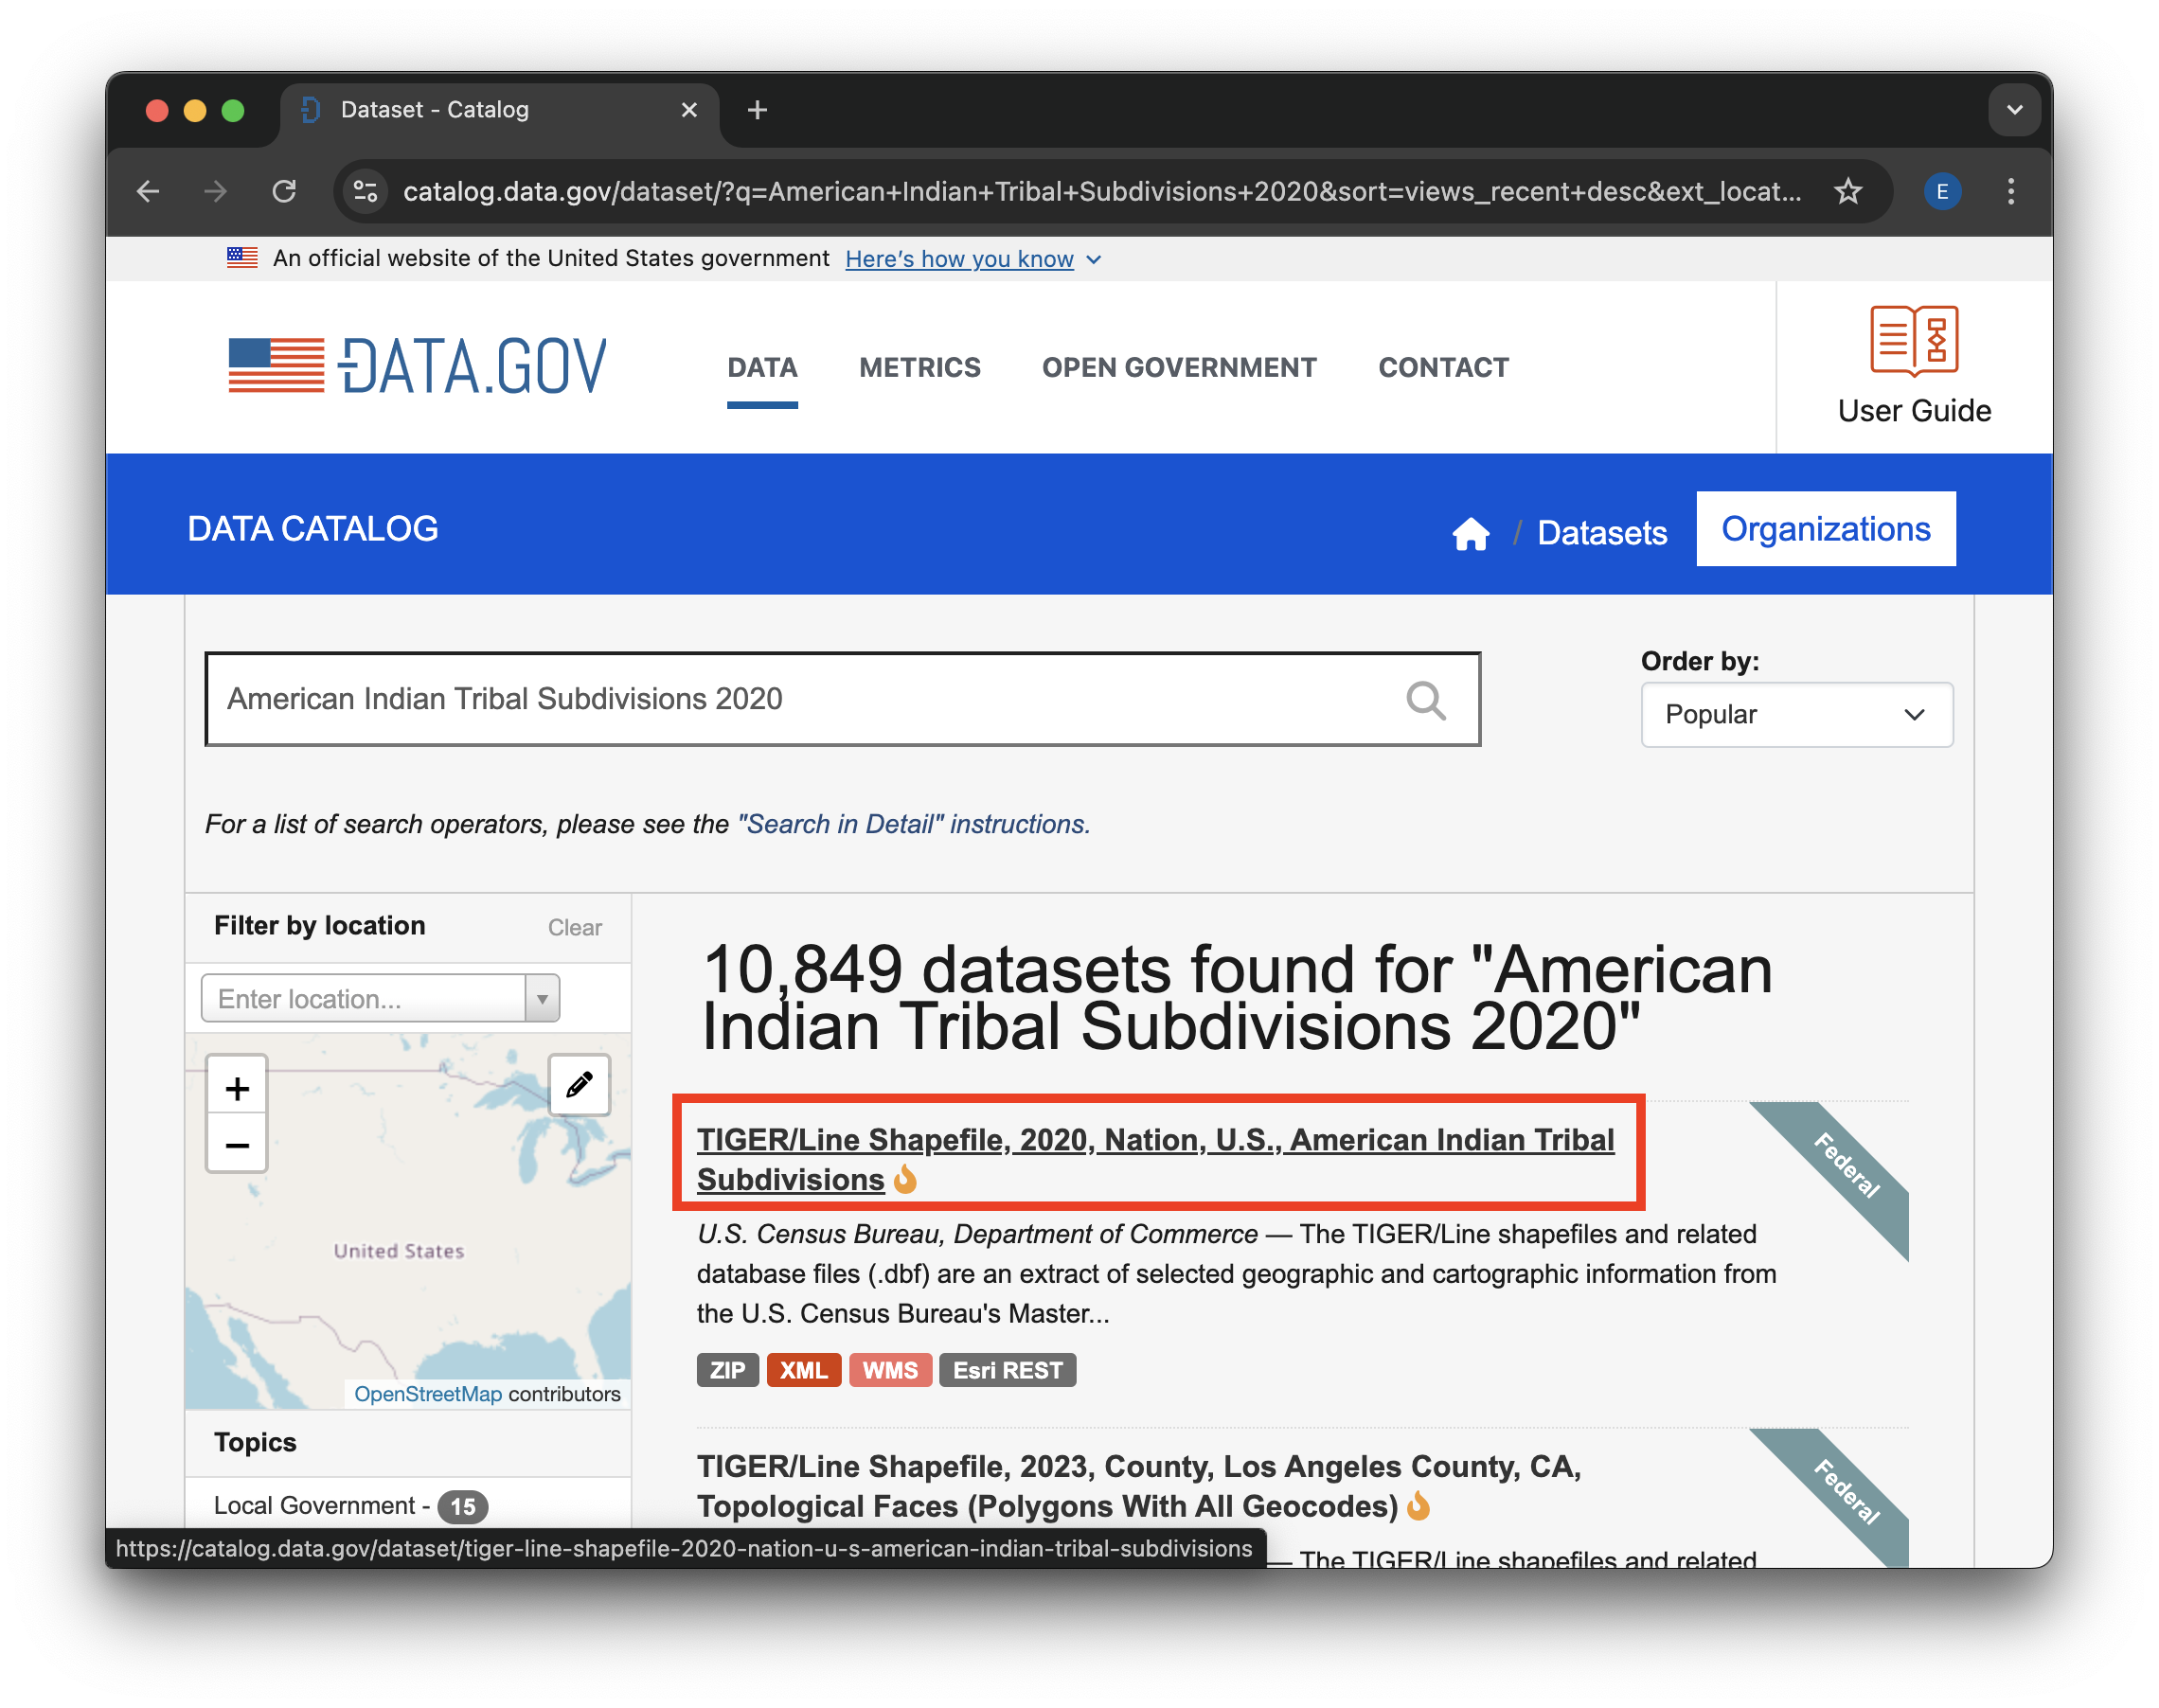
\includegraphics[keepaspectratio]{img/earth-analytics/download/aitsn/03-select.png}}

}

\caption{Select the ``TIGER/Line Shapefile, 2020, Nation, U.S., American
Indian Tribal Subdivisions'' dataset.}

\end{figure}%

\pandocbounded{
\includegraphics[keepaspectratio]{img/earth-analytics/download/aitsn/04-dataset.png}}
\#\# STEP 1D: Download

Next, scroll down to the available files to download. Click on the
\texttt{Download} button for the \texttt{.zip} file -- this will be the
easiest one to open in Python.

\begin{figure}[H]

{\centering \pandocbounded{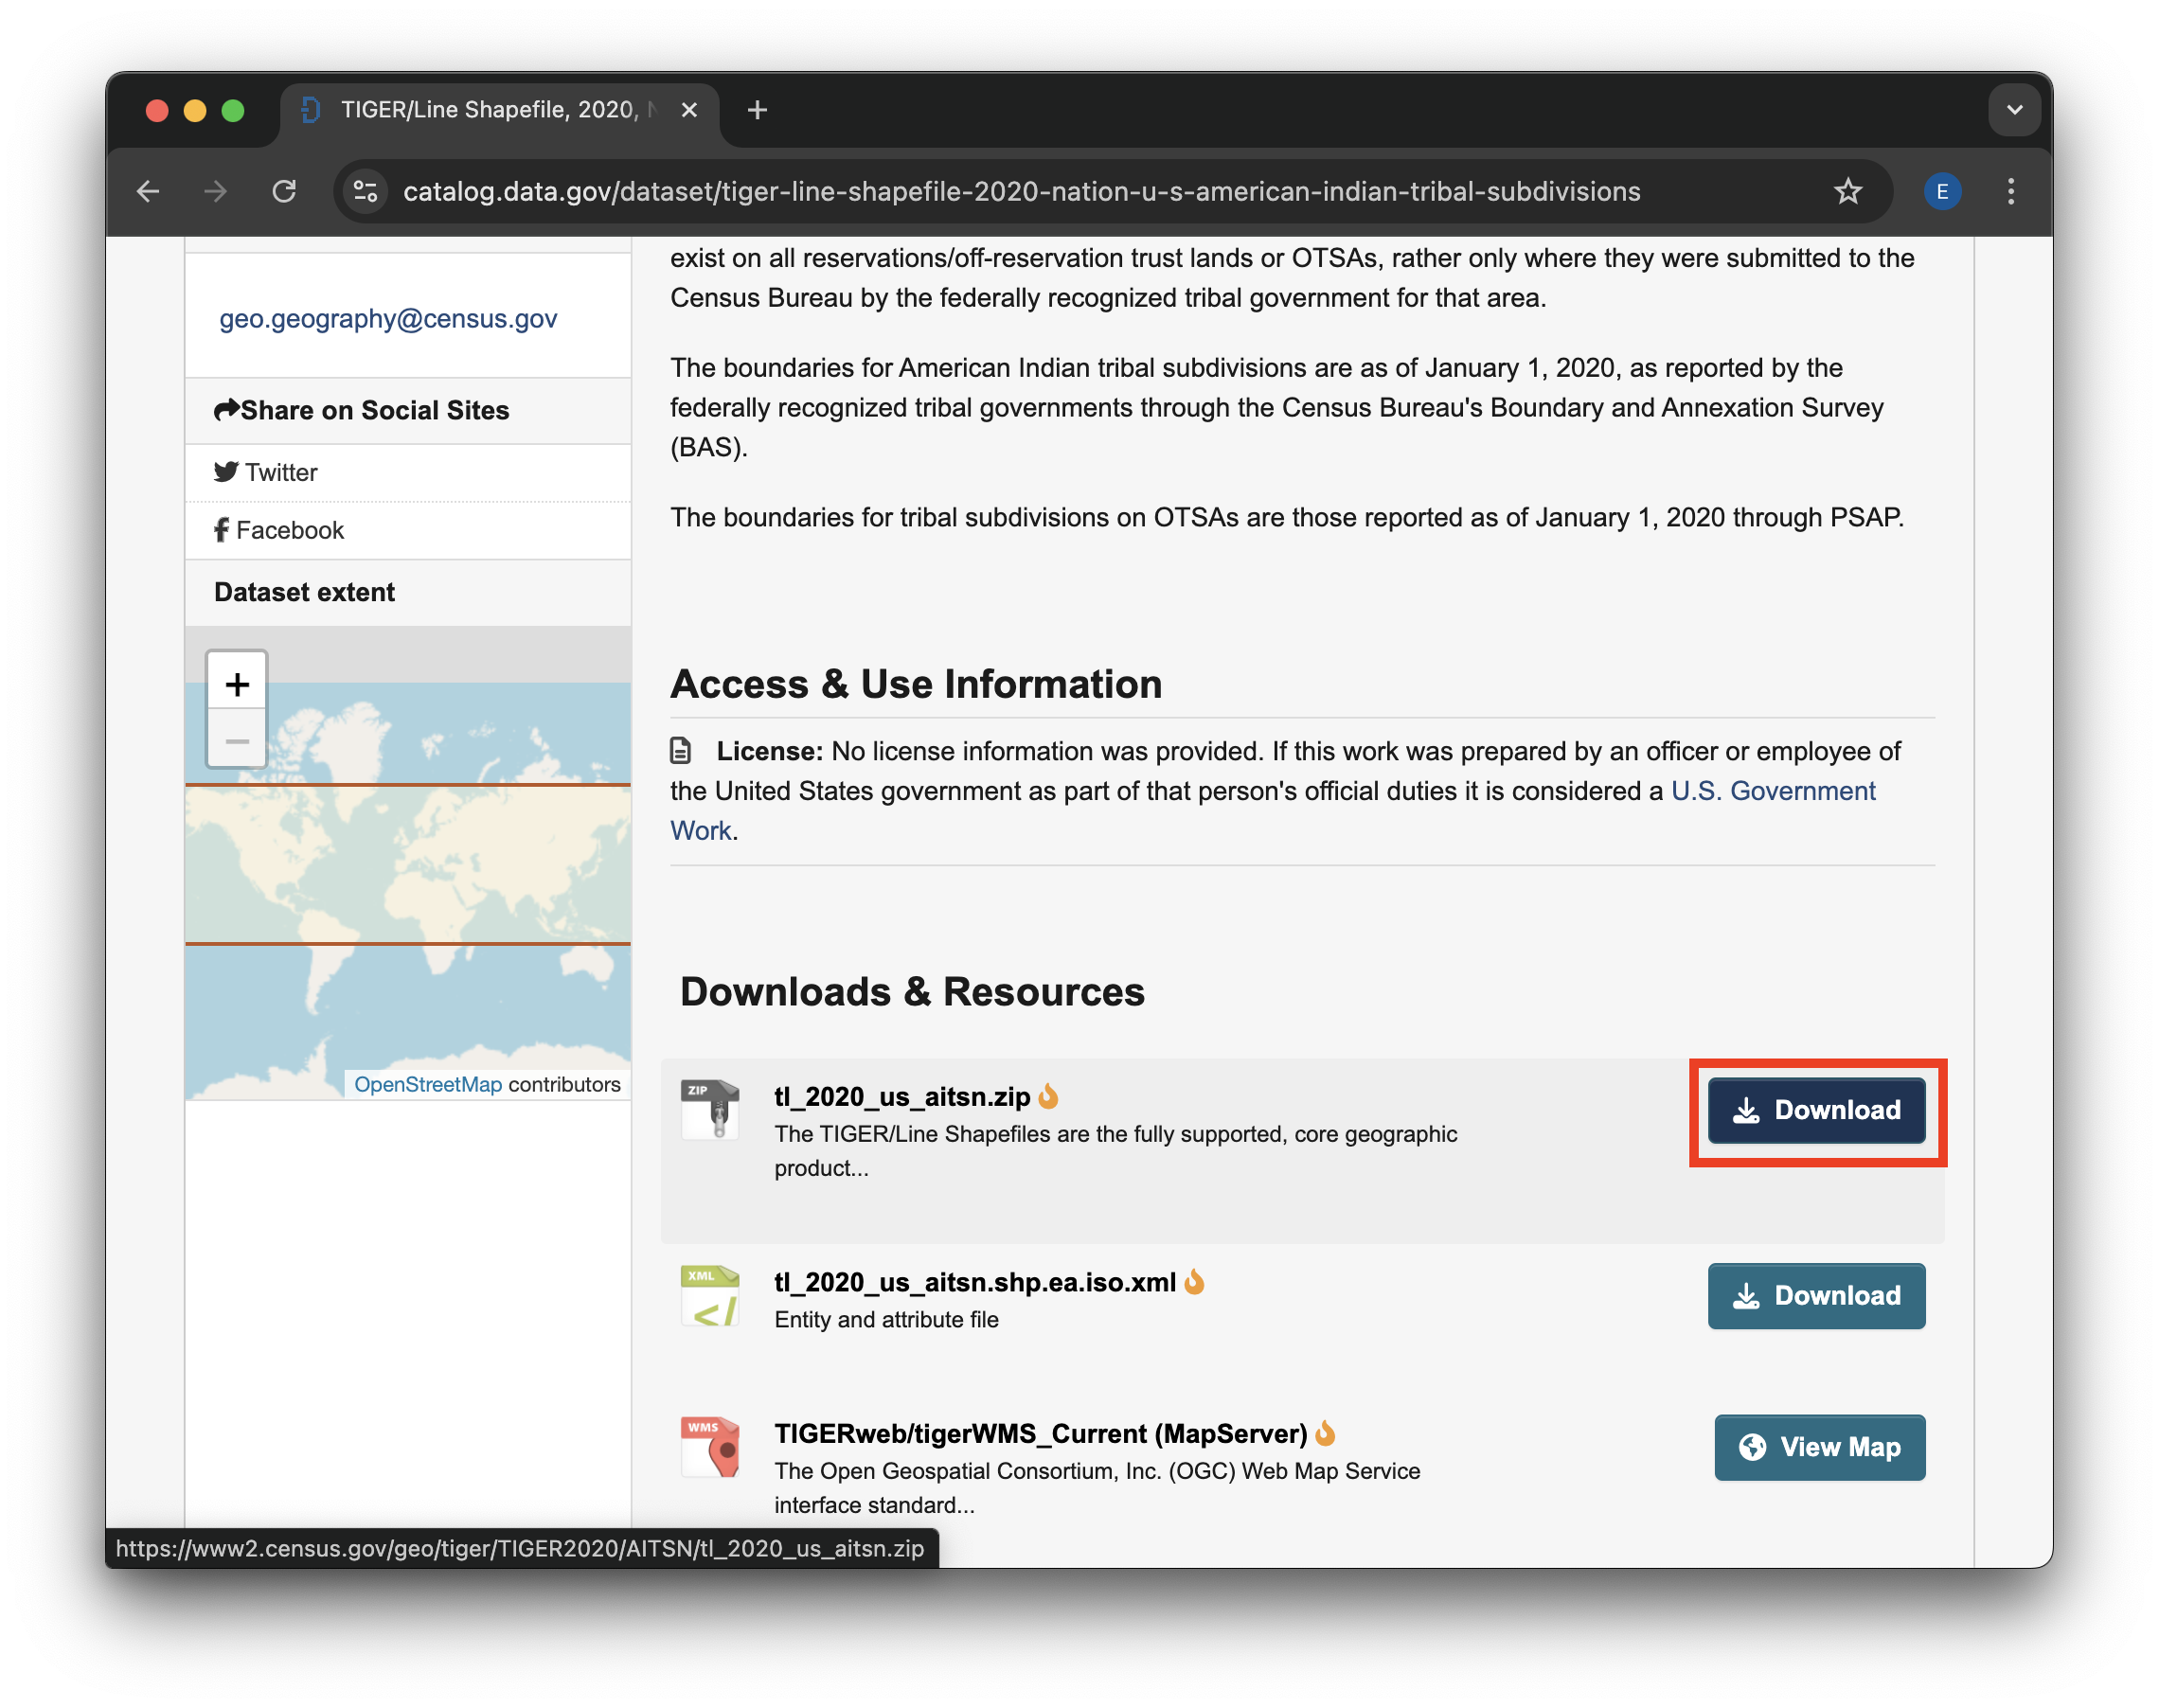
\includegraphics[keepaspectratio]{img/earth-analytics/download/aitsn/05-download.png}}

}

\caption{Scroll down and click on the \texttt{.zip} file
\texttt{Download} button.}

\end{figure}%

\section{STEP 1E: Move your file}\label{step-1e-move-your-file}

We now need to locate the file you downloaded and put it somewhere where
Python can find it. Ideally, you should put the downloaded \texttt{.zip}
file in your project directory. Most web browsers will pop up with some
kind of button to open up your File Explorer (Windows) or Finder (Mac)
in the location of your downloaded files. You can also check in your
user home directory for a \texttt{Downloads} folder. If none of that
works, try opening up your File Explorer/Finder and searching for the
file

\pandocbounded{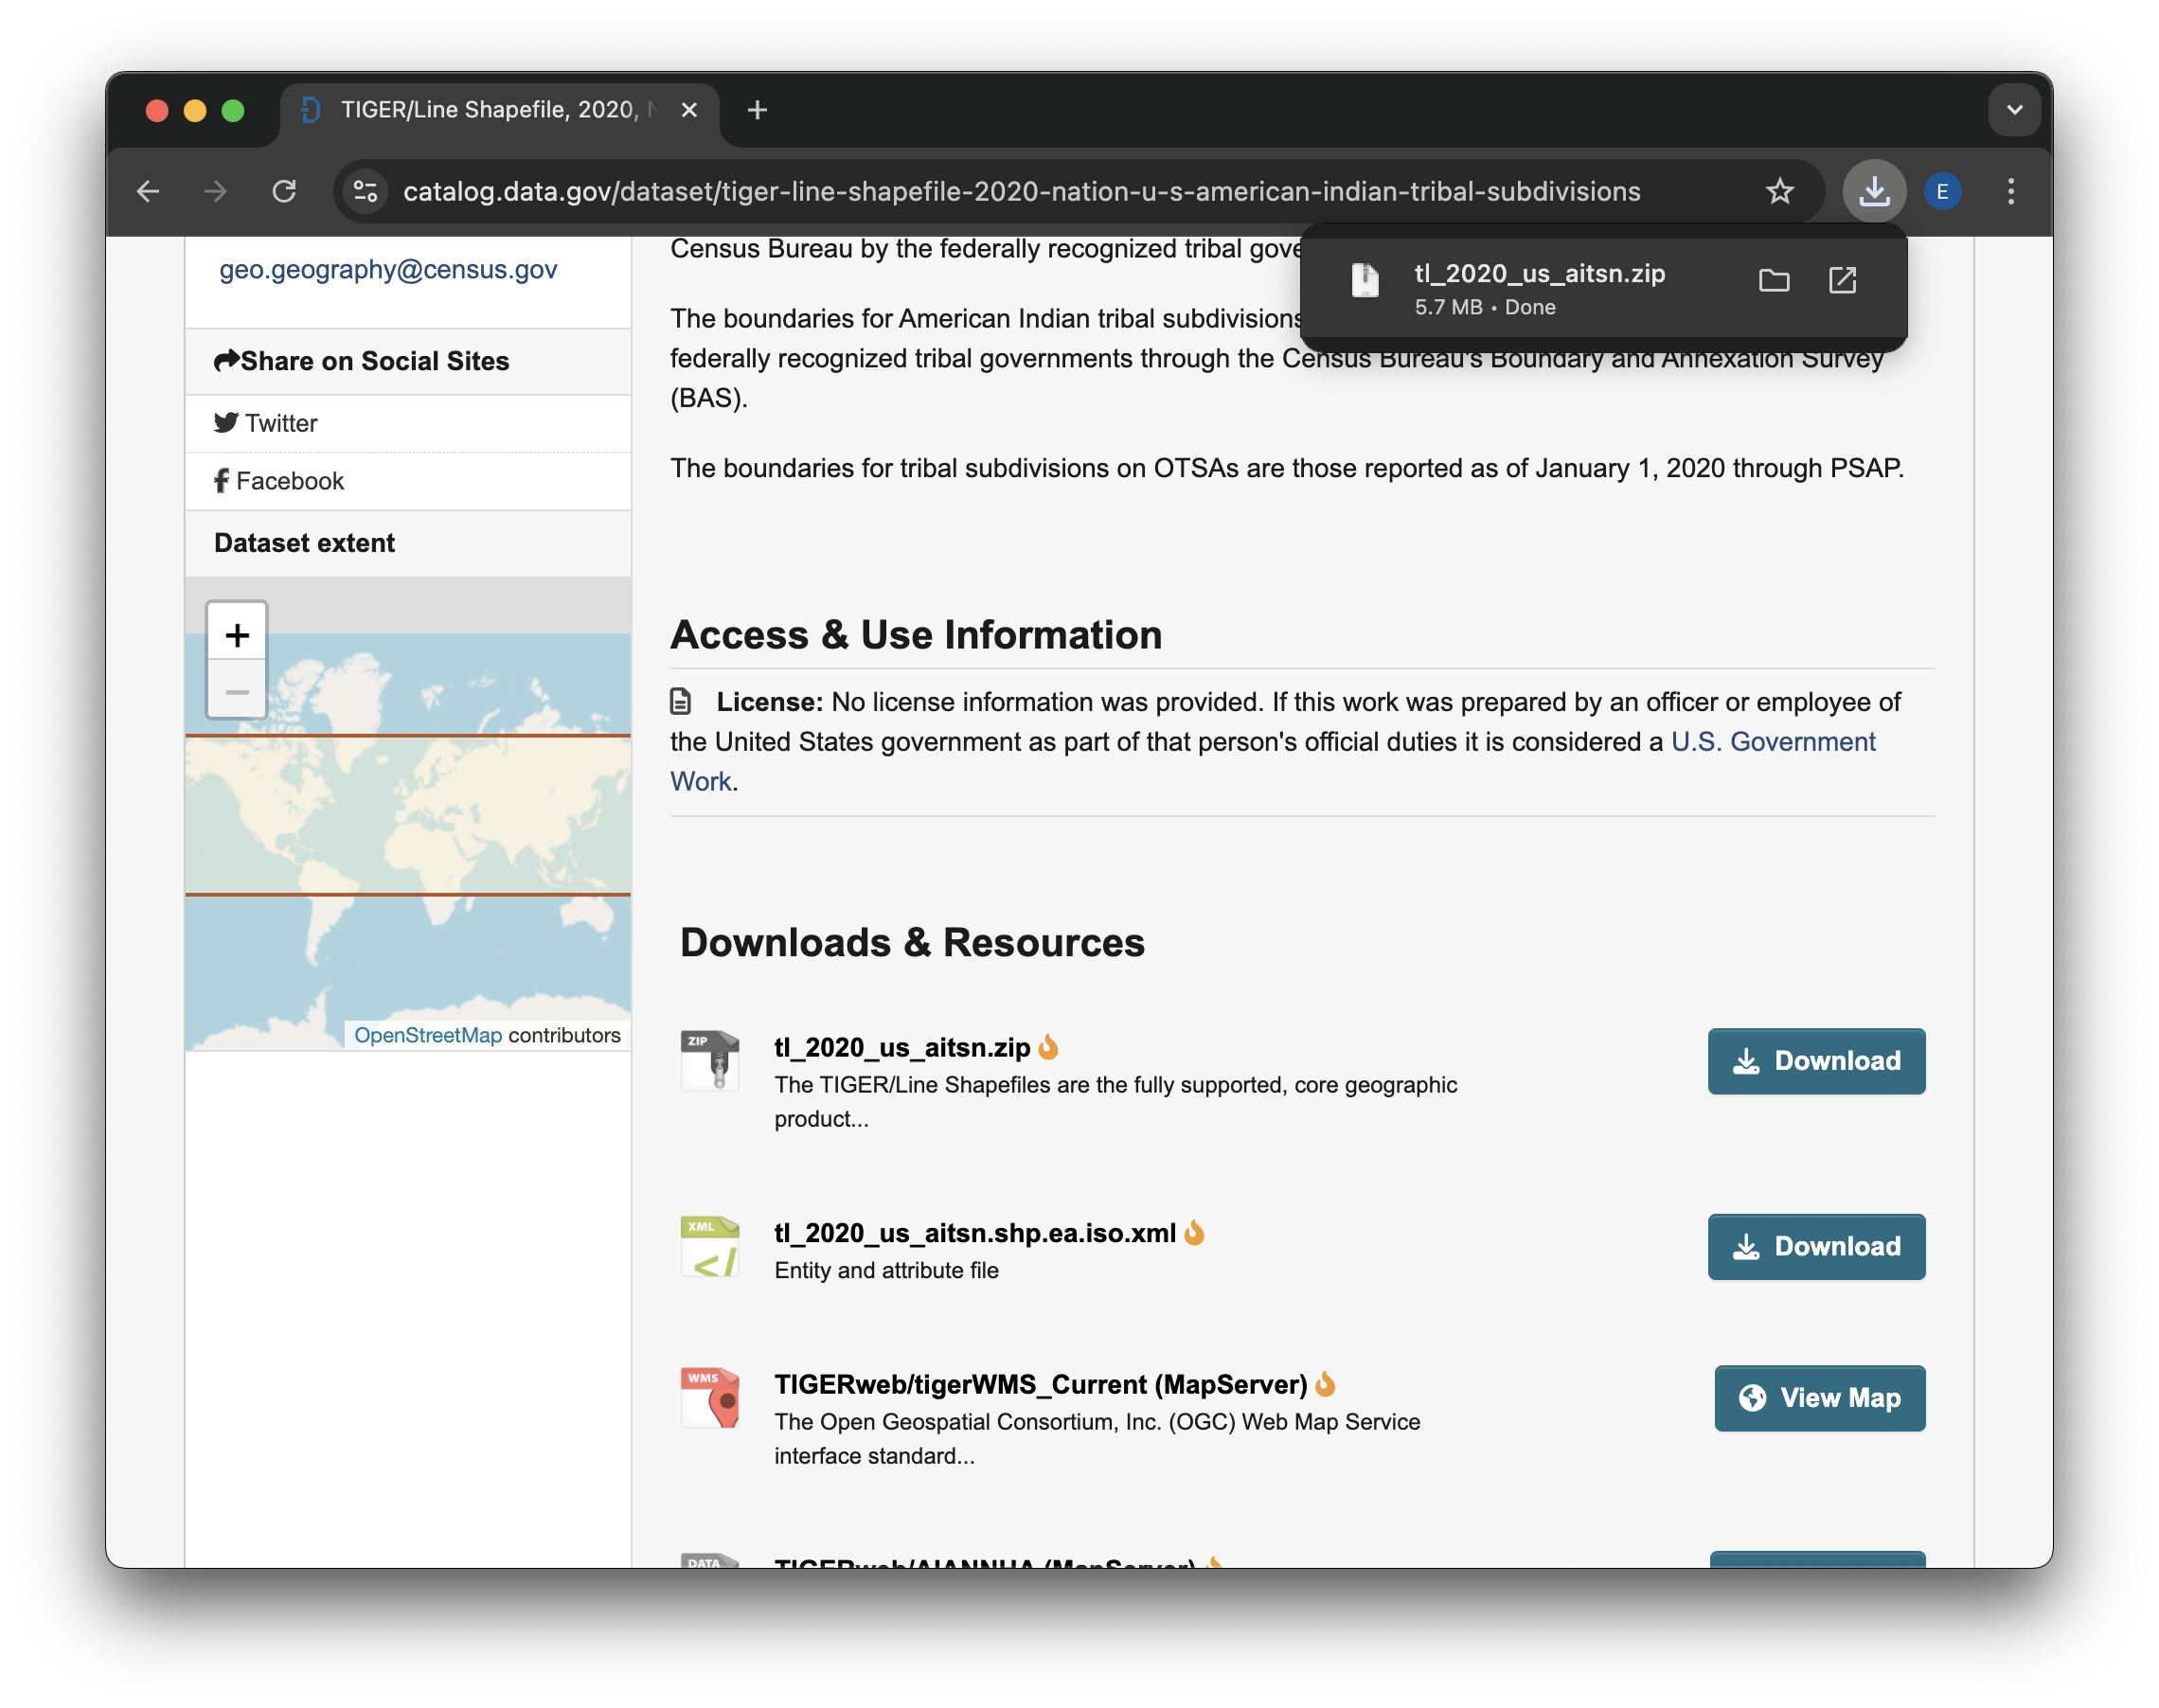
\includegraphics[keepaspectratio]{img/earth-analytics/download/aitsn/06-open-folder.png}}
\pandocbounded{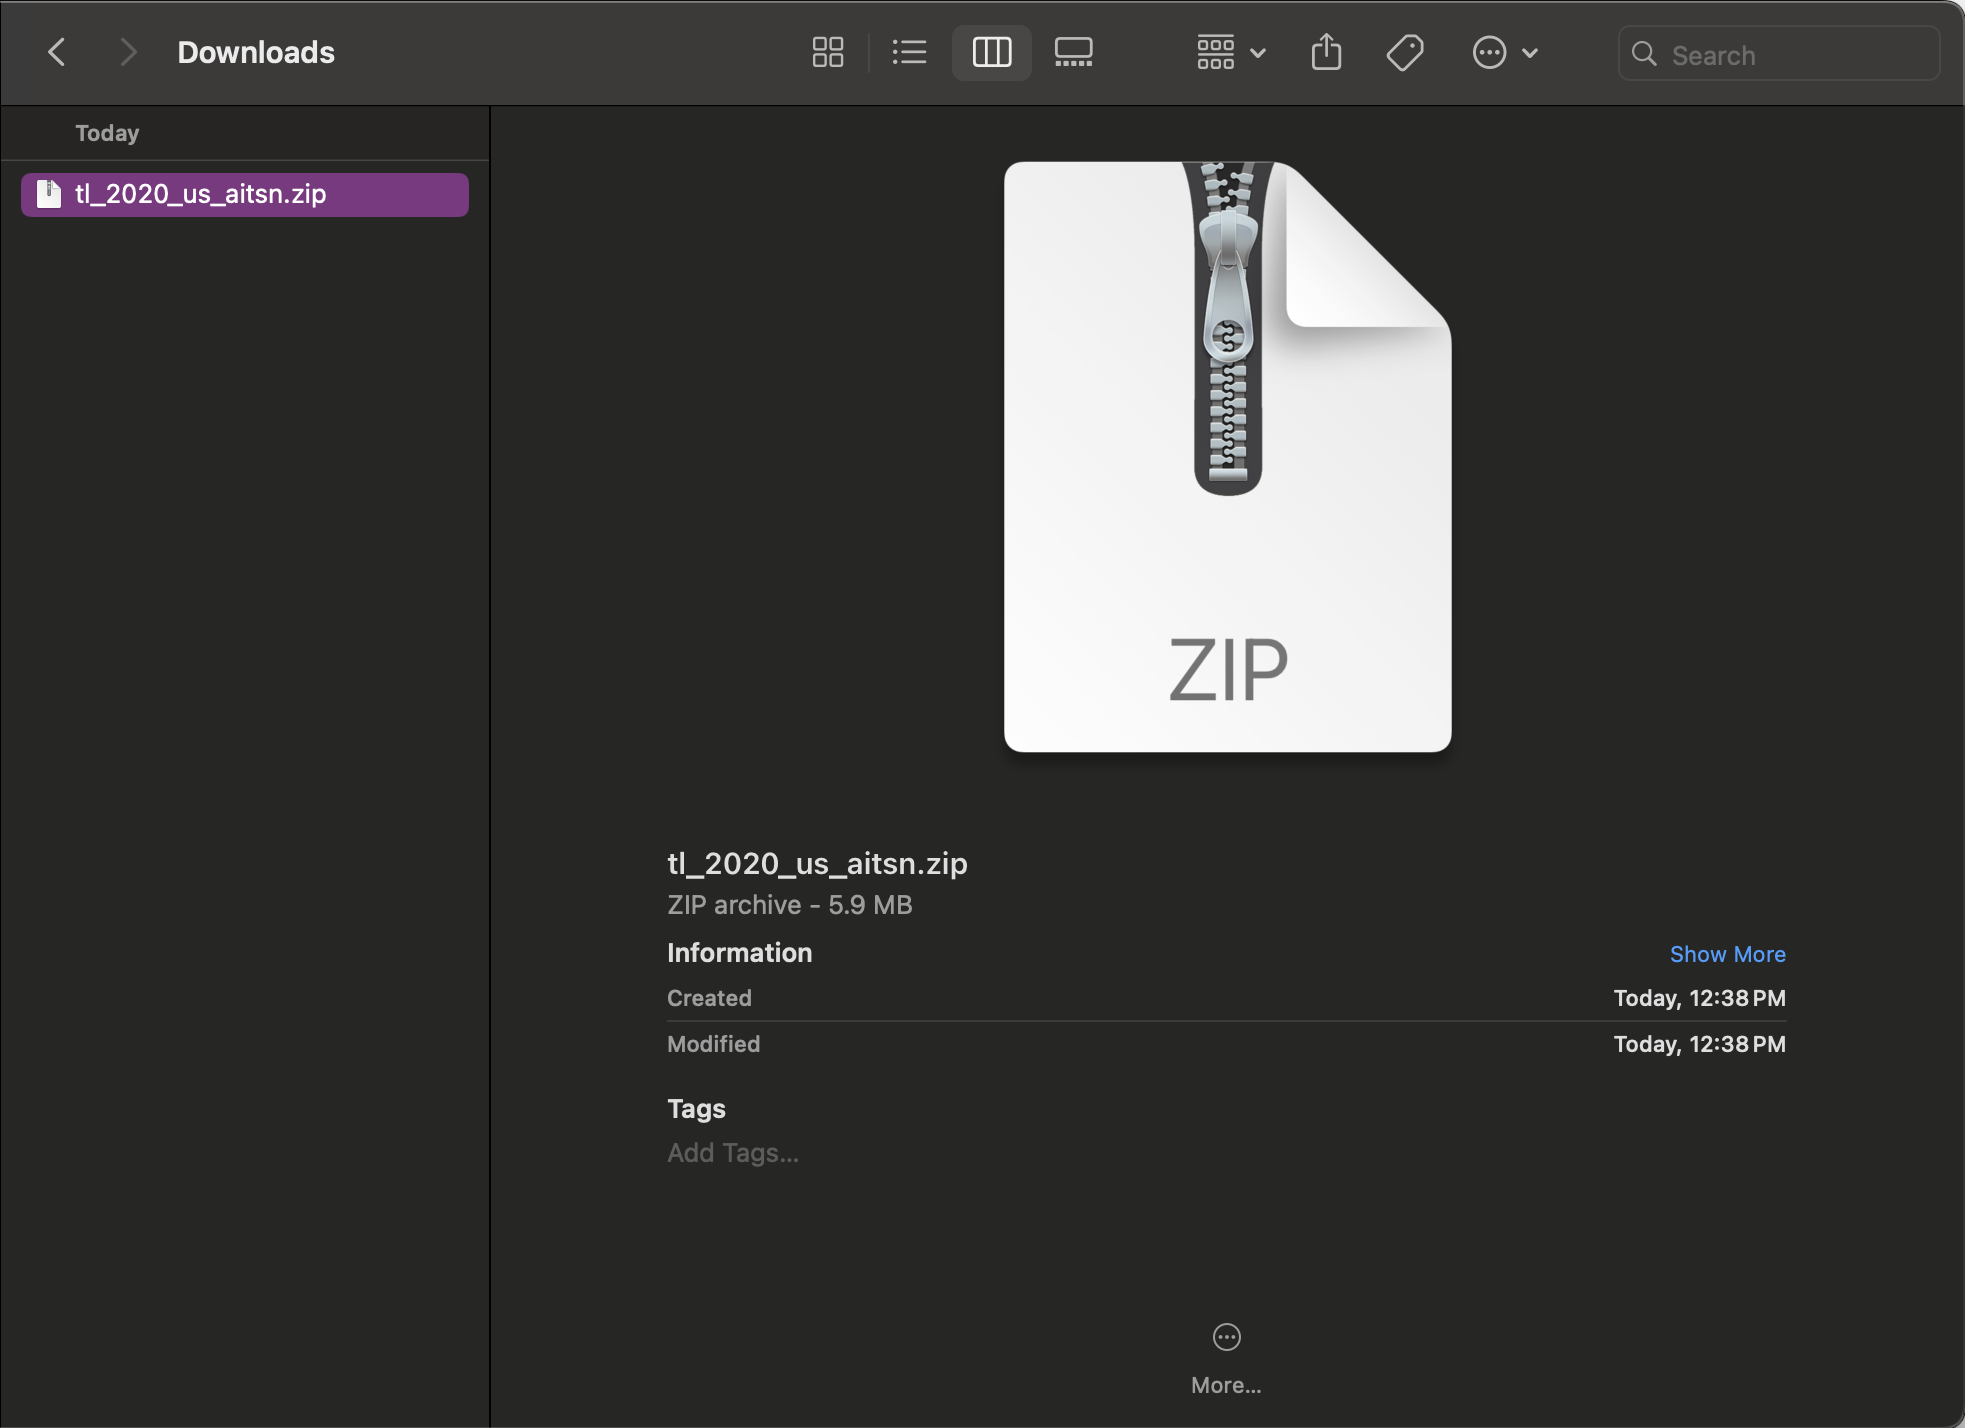
\includegraphics[keepaspectratio]{img/earth-analytics/download/aitsn/07-view.png}}

If you are working on GitHub Codespaces, you will need to upload your
file before relocating it:

\begin{enumerate}
\def\labelenumi{\arabic{enumi}.}
\tightlist
\item
  Go to the \texttt{Explorer} tab in your Codespace
\item
  Right-click on the \texttt{data} folder
\item
  Click \texttt{Upload}
\item
  Select the \texttt{.zip} file you just downloaded.
\end{enumerate}

\begin{figure}[H]

{\centering \pandocbounded{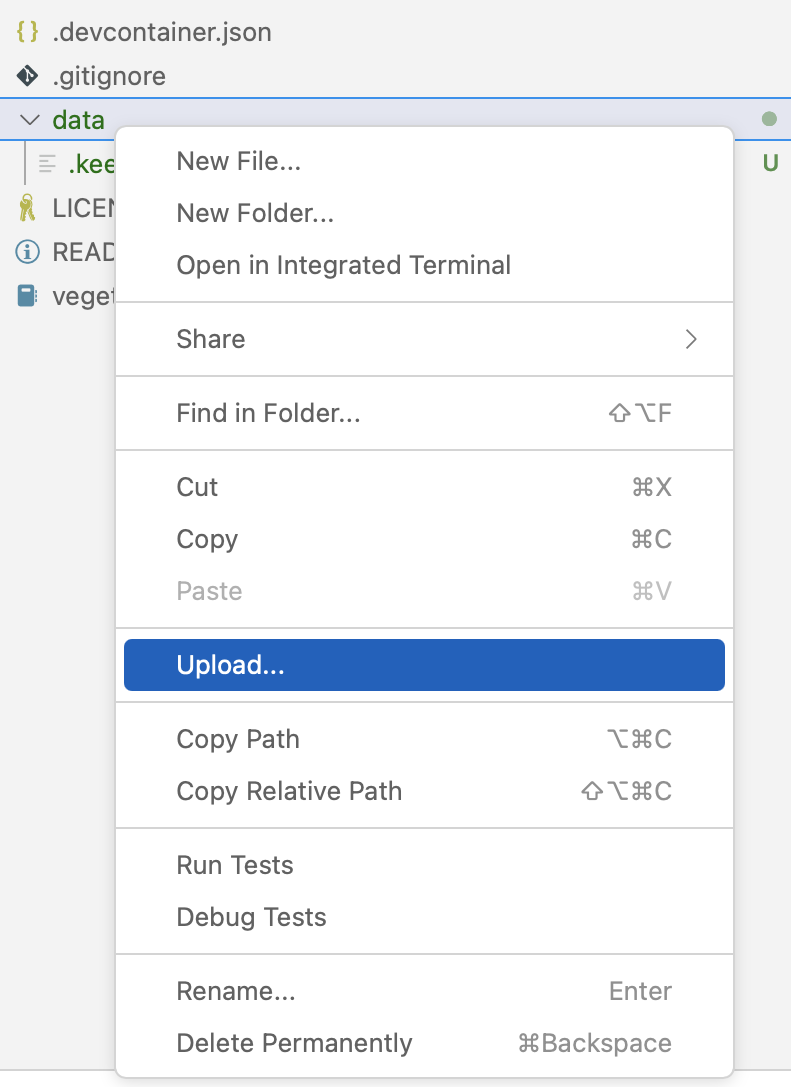
\includegraphics[keepaspectratio]{img/earth-analytics/download/aitsn/08-upload.png}}

}

\caption{If you are using GitHub Codespaces, upload the file.}

\end{figure}%

If you are working in GitHub Codespaces, you can skip ahead to unzipping
the file! If not, you'll need to relocate your file on your computer.
One way to do that is with \textbf{bash}.

\begin{tcolorbox}[enhanced jigsaw, colbacktitle=quarto-callout-color!10!white, opacityback=0, bottomtitle=1mm, toptitle=1mm, bottomrule=.15mm, left=2mm, colframe=quarto-callout-color-frame, leftrule=.75mm, opacitybacktitle=0.6, colback=white, rightrule=.15mm, toprule=.15mm, breakable, titlerule=0mm, title=\textcolor{quarto-callout-color}{\faInfo}\hspace{0.5em}{Try It}, coltitle=black, arc=.35mm]

The code cell below is using a language called \textbf{bash}, which can
be used to move files around your computer. To do that, we're using the
\texttt{cp} command, which stands for \textbf{copy}. In bash, you
indicate that you want to retrieve a variable with the \texttt{\$}
character. Since we're in a Jupyter notebook, we can also access Python
variables this way!

\begin{enumerate}
\def\labelenumi{\arabic{enumi}.}
\tightlist
\item
  Check that the path to your file,
  \texttt{\textasciitilde{}/Downloads/tl\_2020\_us\_aitsn.zip} is
  accurate, and change it if it isn't
\item
  Run the cell to move your file.
\end{enumerate}

\end{tcolorbox}

\begin{Shaded}
\begin{Highlighting}[]
\OperatorTok{!}\NormalTok{cp }\OperatorTok{\textasciitilde{}/}\NormalTok{Downloads}\OperatorTok{/}\NormalTok{tl\_2020\_us\_aitsn.}\BuiltInTok{zip} \OperatorTok{{-}}\NormalTok{d }\StringTok{"$project.project\_dir"}
\end{Highlighting}
\end{Shaded}

\begin{verbatim}
cp: /Users/elsa/Downloads/tl_2020_us_aitsn.zip: No such file or directory
cp: -d: No such file or directory
\end{verbatim}

Now, let's check that the file got moved.

\begin{Shaded}
\begin{Highlighting}[]
\OperatorTok{!}\NormalTok{ls }\StringTok{"$project.project\_dir"}
\end{Highlighting}
\end{Shaded}

\begin{verbatim}
figshare-upload      tl_2020_us_aitsn
gila-river-ndvi      tl_2020_us_aitsn.zip
\end{verbatim}

You can optionally unzip the file. \texttt{geopandas} will be able to
read this particular shapefile from a \texttt{.zip} archive, but some
other files may need to be unzipped. We'll first define the path in
Python, and then use bash to unzip. You can also unzip with the
\texttt{Python} \texttt{zipfile} library, but it is more complicated
than we need right now.

\begin{Shaded}
\begin{Highlighting}[]
\NormalTok{filename }\OperatorTok{=} \StringTok{"tl\_2020\_us\_aitsn"}
\NormalTok{zip\_path }\OperatorTok{=}\NormalTok{ project.project\_dir }\OperatorTok{/} \SpecialStringTok{f"}\SpecialCharTok{\{}\NormalTok{filename}\SpecialCharTok{\}}\SpecialStringTok{.zip"}
\NormalTok{unzip\_dir }\OperatorTok{=}\NormalTok{ project.project\_dir }\OperatorTok{/}\NormalTok{ filename}
\end{Highlighting}
\end{Shaded}

The following command unzips a zip archive to the specified directory
(\texttt{-d}). Any files that already exist are skipped without
prompting (\texttt{-n})

\begin{Shaded}
\begin{Highlighting}[]
\OperatorTok{!}\NormalTok{unzip }\OperatorTok{{-}}\NormalTok{n }\StringTok{"$zip\_path"} \OperatorTok{{-}}\NormalTok{d }\StringTok{"$unzip\_dir"}
\end{Highlighting}
\end{Shaded}

\begin{verbatim}
Archive:  /Users/elsa/Library/Application Support/earth-analytics/gila-river/tl_2020_us_aitsn.zip
\end{verbatim}

You can also delete the zip file, now that it is extracted. This will
help keep your data directory tidy:

\begin{Shaded}
\begin{Highlighting}[]
\OperatorTok{!}\NormalTok{rm }\StringTok{"$zip\_path"}
\end{Highlighting}
\end{Shaded}

\section{STEP 1F: Open boundary in
Python}\label{step-1f-open-boundary-in-python}

\begin{tcolorbox}[enhanced jigsaw, colbacktitle=quarto-callout-color!10!white, opacityback=0, bottomtitle=1mm, toptitle=1mm, bottomrule=.15mm, left=2mm, colframe=quarto-callout-color-frame, leftrule=.75mm, opacitybacktitle=0.6, colback=white, rightrule=.15mm, toprule=.15mm, breakable, titlerule=0mm, title=\textcolor{quarto-callout-color}{\faInfo}\hspace{0.5em}{Try It}, coltitle=black, arc=.35mm]

\begin{enumerate}
\def\labelenumi{\arabic{enumi}.}
\tightlist
\item
  Replace \texttt{"directory-name"} with the actual name of the file you
  downloaded (or the folder you unzipped to) and put in your project
  directory.
\item
  Modify the code below to use \textbf{descriptive variable names}. Feel
  free to refer back to previous challenges for similar code!
\item
  Add a line of code to open up the data path. What library and function
  do you need to open this type of data?
\item
  Add some code to check your data, either by viewing it or making a
  quick plot. Does it look like what you expected?
\end{enumerate}

\end{tcolorbox}

\begin{Shaded}
\begin{Highlighting}[]
\CommentTok{\# Define boundary path}
\NormalTok{path }\OperatorTok{=}\NormalTok{ project.project\_dir }\OperatorTok{/} \StringTok{"directory{-}name"}

\CommentTok{\# Open the site boundary}


\CommentTok{\# Check that the data were downloaded correctly}
\end{Highlighting}
\end{Shaded}

Let's go ahead and select the Gila River subdivisions, and make a site
map.

\begin{tcolorbox}[enhanced jigsaw, colbacktitle=quarto-callout-color!10!white, opacityback=0, bottomtitle=1mm, toptitle=1mm, bottomrule=.15mm, left=2mm, colframe=quarto-callout-color-frame, leftrule=.75mm, opacitybacktitle=0.6, colback=white, rightrule=.15mm, toprule=.15mm, breakable, titlerule=0mm, title=\textcolor{quarto-callout-color}{\faInfo}\hspace{0.5em}{Try It}, coltitle=black, arc=.35mm]

\begin{enumerate}
\def\labelenumi{\arabic{enumi}.}
\tightlist
\item
  Replace \texttt{identifier} with the value you found from exploring
  the interactive map. Make sure that you are using the correct
  \textbf{data type}!
\item
  Change the plot to have a web tile basemap, and look the way you want
  it to.
\end{enumerate}

\end{tcolorbox}

\begin{Shaded}
\begin{Highlighting}[]
\CommentTok{\# Select and merge the subdivisions you want}

\CommentTok{\# Plot the results with web tile images}
\end{Highlighting}
\end{Shaded}

\begin{Shaded}
\begin{Highlighting}[]
\CommentTok{\# Select and merge the subdivisions you want}
\NormalTok{boundary\_gdf }\OperatorTok{=}\NormalTok{ aitsn\_gdf.loc[aitsn\_gdf.AIANNHCE}\OperatorTok{==}\StringTok{\textquotesingle{}1310\textquotesingle{}}\NormalTok{].dissolve()}
\CommentTok{\# Plot the results with web tile images}
\NormalTok{boundary\_gdf.hvplot(}
\NormalTok{    geo}\OperatorTok{=}\VariableTok{True}\NormalTok{, tiles}\OperatorTok{=}\StringTok{\textquotesingle{}EsriImagery\textquotesingle{}}\NormalTok{,}
\NormalTok{    fill\_color}\OperatorTok{=}\VariableTok{None}\NormalTok{, line\_color}\OperatorTok{=}\StringTok{\textquotesingle{}black\textquotesingle{}}\NormalTok{,}
\NormalTok{    title}\OperatorTok{=}\NormalTok{site\_name,}
\NormalTok{    frame\_width}\OperatorTok{=}\DecValTok{500}\NormalTok{)}
\end{Highlighting}
\end{Shaded}

\begin{verbatim}
:Overlay
   .WMTS.I     :WMTS   [Longitude,Latitude]
   .Polygons.I :Polygons   [Longitude,Latitude]
\end{verbatim}

\bookmarksetup{startatroot}

\chapter{STEP 2: AppEEARS API}\label{step-2-appeears-api}

\section{Exploring the AppEEARS API for NASA Earthdata
access}\label{exploring-the-appeears-api-for-nasa-earthdata-access}

Before you get started with the data download today, you will need a
free \href{https://urs.earthdata.nasa.gov/home}{NASA Earthdata account}
if you don't have one already!

Over the next four cells, you will download MODIS NDVI data for the
study period. MODIS is a multispectral instrument that measures Red and
NIR data (and so can be used for NDVI). There are two MODIS sensors on
two different platforms: satellites Terra and Aqua.

\begin{tcolorbox}[enhanced jigsaw, colbacktitle=quarto-callout-color!10!white, opacityback=0, bottomtitle=1mm, toptitle=1mm, bottomrule=.15mm, left=2mm, colframe=quarto-callout-color-frame, leftrule=.75mm, opacitybacktitle=0.6, colback=white, rightrule=.15mm, toprule=.15mm, breakable, titlerule=0mm, title=\textcolor{quarto-callout-color}{\faInfo}\hspace{0.5em}{Read More}, coltitle=black, arc=.35mm]

\href{https://modis.gsfc.nasa.gov/}{Learn more about MODIS datasets and
the science they support}

\end{tcolorbox}

Since we're asking for a special download that only covers our study
area, we can't just find a link to the data - we have to negotiate with
the data server. We're doing this using the
\href{https://appeears.earthdatacloud.nasa.gov/api/}{APPEEARS} API
(Application Programming Interface). The API makes it possible for you
to request data using code. You can use code from the \texttt{earthpy}
library to handle the API request.

\begin{tcolorbox}[enhanced jigsaw, colbacktitle=quarto-callout-color!10!white, opacityback=0, bottomtitle=1mm, toptitle=1mm, bottomrule=.15mm, left=2mm, colframe=quarto-callout-color-frame, leftrule=.75mm, opacitybacktitle=0.6, colback=white, rightrule=.15mm, toprule=.15mm, breakable, titlerule=0mm, title=\textcolor{quarto-callout-color}{\faInfo}\hspace{0.5em}{Try It}, coltitle=black, arc=.35mm]

Often when we want to do something more complex in coding we find an
example and modify it. This download code is already almost a working
example. Your task will be:

\begin{enumerate}
\def\labelenumi{\arabic{enumi}.}
\tightlist
\item
  Replace the start and end dates in the task parameters. Download data
  from July, when greenery is at its peak in the Northern Hemisphere.
\item
  Replace the year range. You should get 3 years before and after the
  event so you can see the change!
\item
  Replace \texttt{gdf} with the name of \textbf{your} site geodataframe.
\item
  \textbf{Enter your NASA Earthdata username and password when
  prompted.} The prompts can be a little hard to see -- look at the top
  of your screen!
\end{enumerate}

\end{tcolorbox}

\begin{tcolorbox}[enhanced jigsaw, colbacktitle=quarto-callout-color!10!white, opacityback=0, bottomtitle=1mm, toptitle=1mm, bottomrule=.15mm, left=2mm, colframe=quarto-callout-color-frame, leftrule=.75mm, opacitybacktitle=0.6, colback=white, rightrule=.15mm, toprule=.15mm, breakable, titlerule=0mm, title=\textcolor{quarto-callout-color}{\faInfo}\hspace{0.5em}{Reflect and Respond}, coltitle=black, arc=.35mm]

What would the product and layer name be if you were trying to download
Landsat Surface Temperature Analysis Ready Data (ARD) instead of MODIS
NDVI?

\end{tcolorbox}

\begin{tcolorbox}[enhanced jigsaw, colbacktitle=quarto-callout-important-color!10!white, opacityback=0, bottomtitle=1mm, toptitle=1mm, bottomrule=.15mm, left=2mm, colframe=quarto-callout-important-color-frame, leftrule=.75mm, opacitybacktitle=0.6, colback=white, rightrule=.15mm, toprule=.15mm, breakable, titlerule=0mm, title=\textcolor{quarto-callout-important-color}{\faExclamation}\hspace{0.5em}{Important}, coltitle=black, arc=.35mm]

It can take some time for Appeears to process your request - anything
from a few minutes to a few hours depending on how busy they are. You
can check your progress by:

\begin{enumerate}
\def\labelenumi{\arabic{enumi}.}
\tightlist
\item
  Going to the \href{https://appeears.earthdatacloud.nasa.gov/}{Appeears
  webpage}
\item
  Clicking the \texttt{Explore} tab
\item
  Logging in with your Earthdata account
\end{enumerate}

\end{tcolorbox}

\begin{Shaded}
\begin{Highlighting}[]
\CommentTok{\# Initialize AppeearsDownloader for MODIS NDVI data}
\NormalTok{ndvi\_downloader }\OperatorTok{=}\NormalTok{ eaapp.AppeearsDownloader(}
\NormalTok{    download\_key}\OperatorTok{=}\NormalTok{download\_key,}
\NormalTok{    product}\OperatorTok{=}\StringTok{\textquotesingle{}MOD13Q1.061\textquotesingle{}}\NormalTok{,}
\NormalTok{    layer}\OperatorTok{=}\StringTok{\textquotesingle{}\_250m\_16\_days\_NDVI\textquotesingle{}}\NormalTok{,}
\NormalTok{    start\_date}\OperatorTok{=}\StringTok{\textquotesingle{}01{-}01\textquotesingle{}}\NormalTok{,}
\NormalTok{    end\_date}\OperatorTok{=}\StringTok{\textquotesingle{}01{-}31\textquotesingle{}}\NormalTok{,}
\NormalTok{    recurring}\OperatorTok{=}\VariableTok{True}\NormalTok{,}
\NormalTok{    year\_range}\OperatorTok{=}\NormalTok{[, ],}
\NormalTok{    polygon}\OperatorTok{=}\NormalTok{gdf}
\NormalTok{)}
\CommentTok{\# Download the prepared download {-}{-} this can take some time!}
\NormalTok{ndvi\_downloader.download\_files(cache}\OperatorTok{=}\VariableTok{True}\NormalTok{)}
\end{Highlighting}
\end{Shaded}

\section{Putting it together: Working with multi-file raster datasets in
Python}\label{putting-it-together-working-with-multi-file-raster-datasets-in-python}

Now you need to load all the downloaded files into Python. You may have
noticed that the `earthpy.appears module gives us all the downloaded
file names\ldots but only some of those are the NDVI files we want while
others are quality files that tell us about the confidence in the
dataset. For now, the files we want all have ``NDVI'' in the name.

Let's start by getting all the NDVI file names. You will also need to
extract the date from the filename. Check out
\href{https://www.earthdatascience.org/courses/intro-to-earth-data-science/write-efficient-python-code/loops/data-workflows-with-loops/}{the
lesson on getting information from filenames in the textbook}. We're
using a slightly different method here (the \texttt{.rglob()} or
\textbf{recursive} glob method, which searchs all the directories nested
inside the path), but the principle is the same.

\begin{tcolorbox}[enhanced jigsaw, colbacktitle=quarto-callout-caution-color!10!white, opacityback=0, bottomtitle=1mm, toptitle=1mm, bottomrule=.15mm, left=2mm, colframe=quarto-callout-caution-color-frame, leftrule=.75mm, opacitybacktitle=0.6, colback=white, rightrule=.15mm, toprule=.15mm, breakable, titlerule=0mm, title=\textcolor{quarto-callout-caution-color}{\faFire}\hspace{0.5em}{GOTCHA ALERT!}, coltitle=black, arc=.35mm]

\texttt{glob} doesn't necessarily find files in the order you would
expect. Make sure to \textbf{sort} your file names like it says in the
textbook.

\end{tcolorbox}

\begin{Shaded}
\begin{Highlighting}[]
\CommentTok{\# Get a sorted list of NDVI tif file paths}
\NormalTok{ndvi\_paths }\OperatorTok{=} \BuiltInTok{sorted}\NormalTok{(}\BuiltInTok{list}\NormalTok{(project.project\_dir.rglob(}\StringTok{\textquotesingle{}ndvi{-}pattern\textquotesingle{}}\NormalTok{)))}

\CommentTok{\# Display the first and last three files paths to check the pattern}
\NormalTok{ndvi\_paths[:}\DecValTok{3}\NormalTok{], ndvi\_paths[}\OperatorTok{{-}}\DecValTok{3}\NormalTok{:]}
\end{Highlighting}
\end{Shaded}

\subsection{Repeating tasks in
Python}\label{repeating-tasks-in-python-1}

Now you should have a few dozen files! For each file, you need to:

\begin{itemize}
\tightlist
\item
  Load the file in using the \texttt{rioxarray} library
\item
  Get the date from the file name
\item
  Add the date as a dimension coordinate
\item
  Give your data variable a name
\end{itemize}

You don't want to write out the code for each file! That's a recipe for
\textbf{copy pasta} and errors. Luckily, Python has tools for doing
similar tasks repeatedly. In this case, you'll use one called a
\texttt{for} loop.

There's some code below that uses a \texttt{for} loop in what is called
an \textbf{accumulation pattern} to process each file. That means that
you will save the results of your processing to a list each time you
process the files, and then merge all the arrays in the list.

\begin{tcolorbox}[enhanced jigsaw, colbacktitle=quarto-callout-color!10!white, opacityback=0, bottomtitle=1mm, toptitle=1mm, bottomrule=.15mm, left=2mm, colframe=quarto-callout-color-frame, leftrule=.75mm, opacitybacktitle=0.6, colback=white, rightrule=.15mm, toprule=.15mm, breakable, titlerule=0mm, title=\textcolor{quarto-callout-color}{\faInfo}\hspace{0.5em}{Try It}, coltitle=black, arc=.35mm]

\begin{itemize}
\tightlist
\item
  Look at the file names. How many characters from the end is the date?
  \texttt{doy\_start} and \texttt{doy\_end} are used to extract the day
  of the year (doy) from the file name. You will need to count
  characters from the end and change the values to get the right part of
  the file name. HINT: the index -1 in Python means the last value, -2
  second-to-last, and so on.
\item
  Replace any required variable names with your chosen variable names
\end{itemize}

\end{tcolorbox}

\begin{Shaded}
\begin{Highlighting}[]
\NormalTok{doy\_start }\OperatorTok{=} \OperatorTok{{-}}\DecValTok{1}
\NormalTok{doy\_end }\OperatorTok{=} \OperatorTok{{-}}\DecValTok{1}

\CommentTok{\# Loop through each NDVI image}
\NormalTok{ndvi\_das }\OperatorTok{=}\NormalTok{ []}
\ControlFlowTok{for}\NormalTok{ ndvi\_path }\KeywordTok{in}\NormalTok{ ndvi\_paths:}
    \CommentTok{\# Get date from file name}

    \CommentTok{\# Open dataset}

    \CommentTok{\# Add date dimension and clean up metadata}
\NormalTok{    da }\OperatorTok{=}\NormalTok{ da.assign\_coords(\{}\StringTok{\textquotesingle{}date\textquotesingle{}}\NormalTok{: date\})}
\NormalTok{    da }\OperatorTok{=}\NormalTok{ da.expand\_dims(\{}\StringTok{\textquotesingle{}date\textquotesingle{}}\NormalTok{: }\DecValTok{1}\NormalTok{\})}
\NormalTok{    da.name }\OperatorTok{=} \StringTok{\textquotesingle{}NDVI\textquotesingle{}}

    \CommentTok{\# Prepare for concatenation}
\end{Highlighting}
\end{Shaded}

\begin{tcolorbox}[enhanced jigsaw, colbacktitle=quarto-callout-color!10!white, opacityback=0, bottomtitle=1mm, toptitle=1mm, bottomrule=.15mm, left=2mm, colframe=quarto-callout-color-frame, leftrule=.75mm, opacitybacktitle=0.6, colback=white, rightrule=.15mm, toprule=.15mm, breakable, titlerule=0mm, title=\textcolor{quarto-callout-color}{\faInfo}\hspace{0.5em}{Try It}, coltitle=black, arc=.35mm]

Next, stack your arrays by date into a time series:

\begin{enumerate}
\def\labelenumi{\arabic{enumi}.}
\tightlist
\item
  Modify the code to match your prior workflow steps and to use
  descriptive variable names
\item
  Replace \texttt{coordinate\_name} with the actual name of the
  coordinate you want to build up.
\end{enumerate}

\end{tcolorbox}

\begin{Shaded}
\begin{Highlighting}[]
\CommentTok{\# Combine NDVI images from all dates}
\NormalTok{da }\OperatorTok{=}\NormalTok{ xr.combine\_by\_coords(list\_of\_data\_arrays, coords}\OperatorTok{=}\NormalTok{[}\StringTok{\textquotesingle{}coordinate\_name\textquotesingle{}}\NormalTok{])}
\NormalTok{da}
\end{Highlighting}
\end{Shaded}

\section{Your turn! Repeat this workflow in a different time and
place.}\label{your-turn-repeat-this-workflow-in-a-different-time-and-place.}

It's not only irrigation that affects NDVI! You could look at:

\begin{itemize}
\tightlist
\item
  Recovery after a national disaster, like a wildfire or hurricane
\item
  Drought
\item
  Deforestation
\item
  Irrigation
\item
  Beaver reintroduction
\end{itemize}

\bookmarksetup{startatroot}

\chapter{Climate Coding Challenge}\label{climate-coding-challenge}

Climate change is impacting the way people live around the world

\hfill\break

\bookmarksetup{startatroot}

\chapter{Part 1: Overview}\label{part-1-overview}

Higher highs, lower lows, storms, and smoke -- we're all feeling the
effects of climate change. In this workflow, you will take a look at
trends in temperature over time in \textbf{?meta:params.location}.

\begin{tcolorbox}[enhanced jigsaw, colbacktitle=quarto-callout-color!10!white, opacityback=0, bottomtitle=1mm, toptitle=1mm, bottomrule=.15mm, left=2mm, colframe=quarto-callout-color-frame, leftrule=.75mm, opacitybacktitle=0.6, colback=white, rightrule=.15mm, toprule=.15mm, breakable, titlerule=0mm, title=\textcolor{quarto-callout-color}{\faInfo}\hspace{0.5em}{Conversation Starter}, coltitle=black, arc=.35mm]

In a few sentences, how is climate change affecting your home?

\end{tcolorbox}

\section{What the fork?! Who wrote
this?}\label{what-the-fork-who-wrote-this}

For this challenge, you'll be running a scientific workflow in Python.
But something's wrong -- The code won't run! Your task is to follow the
instructions below to \textbf{clean and debug} the Python code below so
that it runs.

\begin{tcolorbox}[enhanced jigsaw, colbacktitle=quarto-callout-tip-color!10!white, opacityback=0, bottomtitle=1mm, toptitle=1mm, bottomrule=.15mm, left=2mm, colframe=quarto-callout-tip-color-frame, leftrule=.75mm, opacitybacktitle=0.6, colback=white, rightrule=.15mm, toprule=.15mm, breakable, titlerule=0mm, title=\textcolor{quarto-callout-tip-color}{\faLightbulb}\hspace{0.5em}{Tip}, coltitle=black, arc=.35mm]

Don't worry if you can't solve every bug right away. We'll get there! If
you are working on one bug for more than about 10 minutes, it's time to
ask for help.

\end{tcolorbox}

At the end, you'll \textbf{repeat the workflow} for a location and
measurement of your choosing.

Alright! Let's clean up this code.

Before we get started, let's define some parameters. You can use these
if you want to change how the workflow runs from the top:

\begin{Shaded}
\begin{Highlighting}[]
\BuiltInTok{id} \OperatorTok{=} \StringTok{\textquotesingle{}shortcourse\textquotesingle{}}
\NormalTok{ncei\_filename }\OperatorTok{=} \StringTok{\textquotesingle{}ncei{-}climate{-}karachi.csv\textquotesingle{}}
\NormalTok{project\_name }\OperatorTok{=} \StringTok{\textquotesingle{}Karachi Climate\textquotesingle{}}
\NormalTok{location }\OperatorTok{=} \StringTok{\textquotesingle{}Karachi, Pakistan\textquotesingle{}}
\NormalTok{station\_id }\OperatorTok{=} \StringTok{\textquotesingle{}PKM00041780\textquotesingle{}}
\NormalTok{start\_date }\OperatorTok{=} \StringTok{\textquotesingle{}1942{-}10{-}01\textquotesingle{}}
\NormalTok{end\_date }\OperatorTok{=} \StringTok{\textquotesingle{}2024{-}09{-}30\textquotesingle{}}
\NormalTok{data\_type }\OperatorTok{=} \StringTok{\textquotesingle{}TAVG\textquotesingle{}}
\end{Highlighting}
\end{Shaded}

\bookmarksetup{startatroot}

\chapter{STEP 2: Wrangle your data}\label{step-2-wrangle-your-data}

\section{\texorpdfstring{Python \textbf{packages} let you use code
written by experts around the
world}{Python packages let you use code written by experts around the world}}\label{python-packages-let-you-use-code-written-by-experts-around-the-world}

Because Python is open source, lots of different people and
organizations can contribute (including you!). Many contributions are in
the form of \textbf{packages} which do not come with a standard Python
download.

\begin{tcolorbox}[enhanced jigsaw, colbacktitle=quarto-callout-color!10!white, opacityback=0, bottomtitle=1mm, toptitle=1mm, bottomrule=.15mm, left=2mm, colframe=quarto-callout-color-frame, leftrule=.75mm, opacitybacktitle=0.6, colback=white, rightrule=.15mm, toprule=.15mm, breakable, titlerule=0mm, title=\textcolor{quarto-callout-color}{\faInfo}\hspace{0.5em}{Read More: Packages need to be installed and imported.}, coltitle=black, arc=.35mm]

Learn more about using Python packages. How do you find and use
packages? What is the difference between installing and importing
packages? When do you need to do each one?
\href{https://www.earthdatascience.org/courses/intro-to-earth-data-science/python-code-fundamentals/use-python-packages/}{This
article on Python packages} will walk you through the basics.

\end{tcolorbox}

In the cell below, someone was trying to import the \textbf{pandas
package}, which helps us to work with
\href{https://www.earthdatascience.org/courses/intro-to-earth-data-science/file-formats/use-text-files/}{\textbf{tabular
data} such as comma-separated value or csv files}. But something's
wrong!

\begin{tcolorbox}[enhanced jigsaw, colbacktitle=quarto-callout-color!10!white, opacityback=0, bottomtitle=1mm, toptitle=1mm, bottomrule=.15mm, left=2mm, colframe=quarto-callout-color-frame, leftrule=.75mm, opacitybacktitle=0.6, colback=white, rightrule=.15mm, toprule=.15mm, breakable, titlerule=0mm, title=\textcolor{quarto-callout-color}{\faInfo}\hspace{0.5em}{Try It: Import packages}, coltitle=black, arc=.35mm]

\begin{enumerate}
\def\labelenumi{\arabic{enumi}.}
\tightlist
\item
  Correct the typo below to properly import the pandas package under its
  \textbf{alias} pd.
\item
  Run the cell to import the libraries you'll need for this workflow.
\end{enumerate}

\end{tcolorbox}

\begin{Shaded}
\begin{Highlighting}[]
\CommentTok{\# Import libraries}
\ImportTok{import}\NormalTok{ earthpy}
\ImportTok{import}\NormalTok{ holoviews }\ImportTok{as}\NormalTok{ hv}
\ImportTok{import}\NormalTok{ hvplot.pandas}
\ImportTok{import}\NormalTok{ pandsa }\ImportTok{as}\NormalTok{ pd}
\end{Highlighting}
\end{Shaded}

\section{Download the practice data}\label{download-the-practice-data}

Next, lets download some climate data from
\textbf{?meta:params.location} to practice with.

\begin{enumerate}
\def\labelenumi{\arabic{enumi}.}
\tightlist
\item
  It is surrounded by quotes -- that means Python will interpret it as a
  \texttt{character\ string}, or text, rather than which makes sense for
  a URL.
\item
  The URL is too long to display as one line on most screens. We've put
  parentheses around it so that we can easily split it into multiple
  lines by writing two strings -- one on each line.
\item
  We replaced the figshare identifier for this dataset with
  \texttt{\textquotesingle{}FIGSHARE\_ID\_HERE\textquotesingle{}}.
  You'll have to replace that with the real identifier,
  \textbf{?meta:params.figshare\_id}
\end{enumerate}

However, we still have a problem - we can't get the URL back later on
because it isn't saved in a \textbf{variable}. In other words, we need
to give the url a \textbf{name} so that we can request in from Python
later (sadly, Python has no `hey what was that thingy I typed
yesterday?' function).

\begin{tcolorbox}[enhanced jigsaw, colbacktitle=quarto-callout-color!10!white, opacityback=0, bottomtitle=1mm, toptitle=1mm, bottomrule=.15mm, left=2mm, colframe=quarto-callout-color-frame, leftrule=.75mm, opacitybacktitle=0.6, colback=white, rightrule=.15mm, toprule=.15mm, breakable, titlerule=0mm, title=\textcolor{quarto-callout-color}{\faInfo}\hspace{0.5em}{Read More: Names/variables in Python}, coltitle=black, arc=.35mm]

One of the most common challenges for new programmers is making sure
that your results are stored so you can use them again. In Python, this
is called \textbf{naming}, or saving a \textbf{variable}. Learn more in
this
\href{https://www.earthdatascience.org/courses/intro-to-earth-data-science/python-code-fundamentals/get-started-using-python/variables/}{hands-on
activity on using variables} from our learning portal.

\end{tcolorbox}

\begin{tcolorbox}[enhanced jigsaw, colbacktitle=quarto-callout-color!10!white, opacityback=0, bottomtitle=1mm, toptitle=1mm, bottomrule=.15mm, left=2mm, colframe=quarto-callout-color-frame, leftrule=.75mm, opacitybacktitle=0.6, colback=white, rightrule=.15mm, toprule=.15mm, breakable, titlerule=0mm, title=\textcolor{quarto-callout-color}{\faInfo}\hspace{0.5em}{Try It: Save the URL for later}, coltitle=black, arc=.35mm]

\begin{enumerate}
\def\labelenumi{\arabic{enumi}.}
\tightlist
\item
  Replace \texttt{Project\ Name\ Here} with the actual project name,
  \textbf{?meta:params.project\_name}.
\item
  Replace \texttt{data-folder-name-here} with a \emph{descriptive} name
  for your data folder.
\item
  Run the cell. Can you find the data on your computer?
\end{enumerate}

\end{tcolorbox}

\begin{Shaded}
\begin{Highlighting}[]
\CommentTok{\# Set up project folders}
\NormalTok{project }\OperatorTok{=}\NormalTok{ earthpy.Project(}
    \StringTok{\textquotesingle{}Project Name Here\textquotesingle{}}\NormalTok{,}
\NormalTok{    dirname}\OperatorTok{=}\StringTok{\textquotesingle{}data{-}folder{-}name{-}here\textquotesingle{}}\NormalTok{)}

\CommentTok{\# Download data}
\NormalTok{project.get\_data()}

\CommentTok{\# Check where the data ended up}
\NormalTok{project.project\_dir}
\end{Highlighting}
\end{Shaded}

If you are on GitHub Codespaces, you should be able to see your data in
your \texttt{Explorer} tab.

\begin{figure}[H]

{\centering \pandocbounded{\includegraphics[keepaspectratio]{notebooks/01-climate/.pdf}}

}

\caption{You can find the Explorer tab on the left hand side of the
screen. Your data should be in the \texttt{data} folder mounted there.}

\end{figure}%

You can also take a look at your data using \texttt{bash}, either in
your terminal or here in your Jupyter notebook:

\begin{Shaded}
\begin{Highlighting}[]
\OperatorTok{\%\%}\NormalTok{bash}
\NormalTok{ls $(project.project\_dir)}
\end{Highlighting}
\end{Shaded}

\begin{verbatim}
bash: line 1: project.project_dir: command not found
\end{verbatim}

\begin{verbatim}
_climate-01-machine-readable.qmd
_climate-11-python-as-a-calculator.qmd
_climate-31-overview.qmd
_climate-32-wrangle.qmd
_climate-33-units.qmd
_climate-34-plot.qmd
_climate-35-trend-line.qmd
_climate-98-download.qmd
_climate-99-portfolio.qmd
annual_climate.html
climate-download-css.qmd
climate-download-foundations.qmd
climate-download-shortcourse.qmd
climate-foundations.qmd
climate-shortcourse.qmd
climate-shortcourse.quarto_ipynb
climate-stars.qmd
segments-shortcourse
\end{verbatim}

The \texttt{pandas} library you imported can download data from the
internet directly into a type of Python \textbf{object} called a
\texttt{DataFrame}. In the code cell below, you can see an attempt to do
just this. But there are some problems\ldots{}

\begin{tcolorbox}[enhanced jigsaw, colbacktitle=quarto-callout-color!10!white, opacityback=0, bottomtitle=1mm, toptitle=1mm, bottomrule=.15mm, left=2mm, colframe=quarto-callout-color-frame, leftrule=.75mm, opacitybacktitle=0.6, colback=white, rightrule=.15mm, toprule=.15mm, breakable, titlerule=0mm, title=\textcolor{quarto-callout-color}{\faInfo}\hspace{0.5em}{Try It: Fix some code!}, coltitle=black, arc=.35mm]

\begin{enumerate}
\def\labelenumi{\arabic{enumi}.}
\item
  Leave a space between the \texttt{\#} and text in the comment,
  capitalize it, and try to make it more informative
\item
  Make any changes needed to get this code to run. HINT: The
  \texttt{my\_url} variable doesn't exist - you need to replace it with
  the variable name \textbf{you} chose.
\item
  Modify the \texttt{.read\_csv()} function call to include the
  following parameters:

  \begin{itemize}
  \tightlist
  \item
    \texttt{index\_col=\textquotesingle{}DATE\textquotesingle{}} -- this
    sets the \texttt{DATE} column as the index. Needed for subsetting
    and resampling later on
  \item
    \texttt{parse\_dates=True} -- this lets \texttt{python} know that
    you are working with time-series data, and values in the indexed
    column are \textbf{date time objects}
  \item
    \texttt{na\_values={[}\textquotesingle{}NaN\textquotesingle{}{]}} --
    this lets \texttt{python} know how to handle missing values
  \end{itemize}
\item
  Clean up the code by using \textbf{expressive variable names},
  \textbf{expressive column names}, \textbf{PEP-8 compliant code}, and
  \textbf{descriptive comments}
\end{enumerate}

\end{tcolorbox}

\begin{Shaded}
\begin{Highlighting}[]
\CommentTok{\#download}
\NormalTok{climate\_df }\OperatorTok{=}\NormalTok{ pd.read\_csv(}
\NormalTok{    project.project\_dir }\OperatorTok{/} \StringTok{\textquotesingle{}filename.csv\textquotesingle{}}\NormalTok{,}
    \CommentTok{\#index\_col=\textquotesingle{}something\textquotesingle{})}
\NormalTok{climate\_df}
\end{Highlighting}
\end{Shaded}

\begin{tcolorbox}[enhanced jigsaw, colbacktitle=quarto-callout-tip-color!10!white, opacityback=0, bottomtitle=1mm, toptitle=1mm, bottomrule=.15mm, left=2mm, colframe=quarto-callout-tip-color-frame, leftrule=.75mm, opacitybacktitle=0.6, colback=white, rightrule=.15mm, toprule=.15mm, breakable, titlerule=0mm, title=\textcolor{quarto-callout-tip-color}{\faLightbulb}\hspace{0.5em}{Tip}, coltitle=black, arc=.35mm]

Check out the \texttt{type()} function below - you can use it to check
that your data is now in \texttt{DataFrame} type object.

\end{tcolorbox}

\begin{Shaded}
\begin{Highlighting}[]
\CommentTok{\# Check that the data was imported into a pandas DataFrame}
\BuiltInTok{type}\NormalTok{(climate\_df)}
\end{Highlighting}
\end{Shaded}

\section{\texorpdfstring{Clean up your
\texttt{DataFrame}}{Clean up your DataFrame}}\label{clean-up-your-dataframe}

\begin{tcolorbox}[enhanced jigsaw, colbacktitle=quarto-callout-color!10!white, opacityback=0, bottomtitle=1mm, toptitle=1mm, bottomrule=.15mm, left=2mm, colframe=quarto-callout-color-frame, leftrule=.75mm, opacitybacktitle=0.6, colback=white, rightrule=.15mm, toprule=.15mm, breakable, titlerule=0mm, title=\textcolor{quarto-callout-color}{\faInfo}\hspace{0.5em}{Try It: Get rid of unwanted columns}, coltitle=black, arc=.35mm]

You can use \textbf{double brackets} (\texttt{{[}{[}} and
\texttt{{]}{]}}) to select only the columns that you want from your
\texttt{DataFrame}:

\begin{enumerate}
\def\labelenumi{\arabic{enumi}.}
\tightlist
\item
  Change \texttt{some\_column\_name} to the Temperature column name.
\item
  Give the \texttt{DataFrame} a more descriptive name.
\item
  Add a properly formatted comment to describe what this code is doing.
\end{enumerate}

\end{tcolorbox}

\begin{tcolorbox}[enhanced jigsaw, colbacktitle=quarto-callout-warning-color!10!white, opacityback=0, bottomtitle=1mm, toptitle=1mm, bottomrule=.15mm, left=2mm, colframe=quarto-callout-warning-color-frame, leftrule=.75mm, opacitybacktitle=0.6, colback=white, rightrule=.15mm, toprule=.15mm, breakable, titlerule=0mm, title=\textcolor{quarto-callout-warning-color}{\faExclamationTriangle}\hspace{0.5em}{Warning}, coltitle=black, arc=.35mm]

Column names are text values, not variable names, so you need to put
them in quotes!

\end{tcolorbox}

\begin{Shaded}
\begin{Highlighting}[]
\NormalTok{climate\_df }\OperatorTok{=}\NormalTok{ climate\_df[[}\StringTok{\textquotesingle{}some\_column\_name\textquotesingle{}}\NormalTok{]]}
\NormalTok{climate\_df}
\end{Highlighting}
\end{Shaded}

\bookmarksetup{startatroot}

\chapter{STEP 3: Convert units}\label{step-3-convert-units}

It's important to keep track of the units of all your data. You don't
want to be like the
\href{https://www.latimes.com/archives/la-xpm-1999-oct-01-mn-17288-story.html}{NASA
team who crashed a probe into Mars because different teams used
different units})!

\section{Use labels to keep track of units for you and your
collaborators}\label{use-labels-to-keep-track-of-units-for-you-and-your-collaborators}

One way to keep track of your data's units is to include the unit in
data \textbf{labels}. In the case of a \texttt{DataFrame}, that usually
means the column names.

\begin{tcolorbox}[enhanced jigsaw, colbacktitle=quarto-callout-color!10!white, opacityback=0, bottomtitle=1mm, toptitle=1mm, bottomrule=.15mm, left=2mm, colframe=quarto-callout-color-frame, leftrule=.75mm, opacitybacktitle=0.6, colback=white, rightrule=.15mm, toprule=.15mm, breakable, titlerule=0mm, title=\textcolor{quarto-callout-color}{\faInfo}\hspace{0.5em}{Try It: Add units to your column name}, coltitle=black, arc=.35mm]

A big part of writing \textbf{expressive} code is descriptive labels.
Let's rename the columns of your dataframe to include units. Complete
the following steps:

\begin{enumerate}
\def\labelenumi{\arabic{enumi}.}
\tightlist
\item
  Replace \texttt{dataframe} with the name of \textbf{your}
  \texttt{DataFrame}, and \texttt{dataframe\_units} with an expressive
  new name.
\item
  Check out the
  \href{https://www.ncei.noaa.gov/data/global-historical-climatology-network-daily/doc/GHCND_documentation.pdf}{documentation
  for GCHNd data}. We downloaded data with ``standard'' units; find out
  what that means for both temperature and precipitation.
\item
  Replace \texttt{\textquotesingle{}TOBS\textquotesingle{}} with the
  temperature column name in your data, and
  \texttt{\textquotesingle{}TOBS\_UNIT\textquotesingle{}} with a column
  name that includes the correct unit.
\end{enumerate}

\end{tcolorbox}

\begin{Shaded}
\begin{Highlighting}[]
\NormalTok{dataframe\_units }\OperatorTok{=}\NormalTok{ dataframe.rename(columns}\OperatorTok{=}\NormalTok{\{}
    \StringTok{\textquotesingle{}TOBS\textquotesingle{}}\NormalTok{: }\StringTok{\textquotesingle{}TOBS\_UNIT\textquotesingle{}}\NormalTok{,}
\NormalTok{\})}

\NormalTok{dataframe\_units}
\end{Highlighting}
\end{Shaded}

\section{For scientific applications, it is often useful to have values
in metric
units}\label{for-scientific-applications-it-is-often-useful-to-have-values-in-metric-units}

\begin{tcolorbox}[enhanced jigsaw, colbacktitle=quarto-callout-color!10!white, opacityback=0, bottomtitle=1mm, toptitle=1mm, bottomrule=.15mm, left=2mm, colframe=quarto-callout-color-frame, leftrule=.75mm, opacitybacktitle=0.6, colback=white, rightrule=.15mm, toprule=.15mm, breakable, titlerule=0mm, title=\textcolor{quarto-callout-color}{\faInfo}\hspace{0.5em}{Try It: Convert units}, coltitle=black, arc=.35mm]

The code below attempts to convert the data to Celcius, using Python
mathematical \textbf{operators}, like \texttt{+}, \texttt{-},
\texttt{*}, and \texttt{/}. Mathematical operators in Python work just
like a calculator, and that includes using parentheses to designat the
\textbf{order of operations}. The equation for converting Fahrenheit
temperature to Celcius is:

\[ T_C = (T_F - 32) * \frac{5}{9} \]

This code is not well documented and doesn't follow
\href{https://peps.python.org/pep-0008/\#other-recommendations}{PEP-8
guidelines}, which has caused the author to miss an \textbf{important
error}!

Complete the following steps:

\begin{enumerate}
\def\labelenumi{\arabic{enumi}.}
\tightlist
\item
  Replace \texttt{dataframe} with the name of \textbf{your}
  \texttt{DataFrame}.
\item
  Replace \texttt{\textquotesingle{}old\_temperature\textquotesingle{}}
  with the column name \textbf{you} used; Replace
  \texttt{\textquotesingle{}new\_temperature\textquotesingle{}} with an
  \textbf{expressive} column name.
\item
  \textbf{THERE IS AN ERROR IN THE CONVERSION MATH - Fix it!}
\end{enumerate}

\end{tcolorbox}

\begin{Shaded}
\begin{Highlighting}[]
\NormalTok{dataframe\_units[}\StringTok{\textquotesingle{}new\_temperature\textquotesingle{}}\NormalTok{]}\OperatorTok{=}\NormalTok{ dataframe\_units[}\StringTok{\textquotesingle{}old\_temperature\textquotesingle{}}\NormalTok{]}\OperatorTok{{-}}\DecValTok{32}\OperatorTok{*}\DecValTok{5}\OperatorTok{/}\DecValTok{9}
\NormalTok{dataframe\_units}
\end{Highlighting}
\end{Shaded}

\begin{tcolorbox}[enhanced jigsaw, colbacktitle=quarto-callout-color!10!white, opacityback=0, bottomtitle=1mm, toptitle=1mm, bottomrule=.15mm, left=2mm, colframe=quarto-callout-color-frame, leftrule=.75mm, opacitybacktitle=0.6, colback=white, rightrule=.15mm, toprule=.15mm, breakable, titlerule=0mm, title=\textcolor{quarto-callout-color}{\faInfo}\hspace{0.5em}{Looking for an Extra Challenge?}, coltitle=black, arc=.35mm]

Using the code below as a framework, write and apply a \textbf{function}
that converts to Celcius. You should also rewrite this function name to
be more expressive.

\end{tcolorbox}

\begin{Shaded}
\begin{Highlighting}[]
\CommentTok{\# Convert units with a function}
\KeywordTok{def}\NormalTok{ convert(temperature):}
    \CommentTok{"""Convert temperature to Celcius"""}
    \ControlFlowTok{return}\NormalTok{ temperature }\CommentTok{\# Put your equation in here}

\NormalTok{dataframe[}\StringTok{\textquotesingle{}TEMP\_C\textquotesingle{}}\NormalTok{] }\OperatorTok{=}\NormalTok{ (}
\NormalTok{    dataframe[}\StringTok{\textquotesingle{}TEMP\_F\textquotesingle{}}\NormalTok{].}\BuiltInTok{apply}\NormalTok{(convert))}
\end{Highlighting}
\end{Shaded}

\begin{Shaded}
\begin{Highlighting}[]
\KeywordTok{def}\NormalTok{ convert\_f\_to\_c(temperature\_f):}
    \CommentTok{"""Convert temperature to Celcius"""}
    \ControlFlowTok{return}\NormalTok{ (temperature\_f }\OperatorTok{{-}} \DecValTok{32}\NormalTok{) }\OperatorTok{*} \DecValTok{5}\OperatorTok{/}\DecValTok{9}

\NormalTok{climate\_u\_df[}\StringTok{\textquotesingle{}temp\_c\textquotesingle{}}\NormalTok{] }\OperatorTok{=}\NormalTok{ (}
\NormalTok{    climate\_u\_df[}\StringTok{\textquotesingle{}temp\_f\textquotesingle{}}\NormalTok{].}\BuiltInTok{apply}\NormalTok{(convert\_f\_to\_c))}
\end{Highlighting}
\end{Shaded}

\bookmarksetup{startatroot}

\chapter{STEP 4: Plot your results}\label{step-4-plot-your-results}

\section{Plot the temperature column vs time to explore the
data}\label{plot-the-temperature-column-vs-time-to-explore-the-data}

Plotting in Python is easy, but not quite this easy:

\begin{Shaded}
\begin{Highlighting}[]
\NormalTok{climate\_u\_df.plot()}
\end{Highlighting}
\end{Shaded}

\pandocbounded{\includegraphics[keepaspectratio]{notebooks/01-climate/climate-shortcourse_files/figure-pdf/cell-19-output-1.png}}

Looks like we have \emph{both} temperature units on the same plot, and
it's hard to see what it is because it's missing labels!

\begin{tcolorbox}[enhanced jigsaw, colbacktitle=quarto-callout-tip-color!10!white, opacityback=0, bottomtitle=1mm, toptitle=1mm, bottomrule=.15mm, left=2mm, colframe=quarto-callout-tip-color-frame, leftrule=.75mm, opacitybacktitle=0.6, colback=white, rightrule=.15mm, toprule=.15mm, breakable, titlerule=0mm, title=\textcolor{quarto-callout-tip-color}{\faLightbulb}\hspace{0.5em}{\textbf{Label your plot}}, coltitle=black, arc=.35mm]

\begin{figure}[H]

{\centering \pandocbounded{\includegraphics[keepaspectratio]{index_files/mediabag/convincing.png}}

}

\caption{Source: https://xkcd.com/833}

\end{figure}%

Make sure each plot has:

\begin{itemize}
\tightlist
\item
  A title that explains where and when the data are from
\item
  x- and y- axis labels with \textbf{units} where appropriate
\item
  A legend where appropriate
\end{itemize}

\end{tcolorbox}

When plotting in Python, you'll always need to add some instructions on
labels and how you want your plot to look.

\begin{tcolorbox}[enhanced jigsaw, colbacktitle=quarto-callout-color!10!white, opacityback=0, bottomtitle=1mm, toptitle=1mm, bottomrule=.15mm, left=2mm, colframe=quarto-callout-color-frame, leftrule=.75mm, opacitybacktitle=0.6, colback=white, rightrule=.15mm, toprule=.15mm, breakable, titlerule=0mm, title=\textcolor{quarto-callout-color}{\faInfo}\hspace{0.5em}{Try It: Plot your data}, coltitle=black, arc=.35mm]

\begin{enumerate}
\def\labelenumi{\arabic{enumi}.}
\tightlist
\item
  Change \texttt{dataframe} to \textbf{your} \texttt{DataFrame} name.
\item
  Change \texttt{y=} to the name of your \textbf{temperature} column
  name.
\item
  Use the \texttt{title}, \texttt{ylabel}, and \texttt{xlabel}
  parameters to add key text to your plot.
\item
  Adjust the size of your figure using \texttt{figsize=(x,y)} where
  \texttt{x} is figure width and \texttt{y} is figure height
\end{enumerate}

\end{tcolorbox}

\begin{tcolorbox}[enhanced jigsaw, colbacktitle=quarto-callout-tip-color!10!white, opacityback=0, bottomtitle=1mm, toptitle=1mm, bottomrule=.15mm, left=2mm, colframe=quarto-callout-tip-color-frame, leftrule=.75mm, opacitybacktitle=0.6, colback=white, rightrule=.15mm, toprule=.15mm, breakable, titlerule=0mm, title=\textcolor{quarto-callout-tip-color}{\faLightbulb}\hspace{0.5em}{Tip}, coltitle=black, arc=.35mm]

Labels have to be a \emph{type} in Python called a \textbf{string}. You
can make a string by putting quotes around your label, just like the
column names in the sample code (eg
\texttt{y=\textquotesingle{}temperature\textquotesingle{}}).

\end{tcolorbox}

\begin{Shaded}
\begin{Highlighting}[]
\CommentTok{\# Plot the data using .plot}
\NormalTok{climate\_u\_df.plot(}
\NormalTok{    y}\OperatorTok{=}\StringTok{\textquotesingle{}the\_temperature\_column\textquotesingle{}}\NormalTok{,}
\NormalTok{    title}\OperatorTok{=}\StringTok{\textquotesingle{}Title Goes Here\textquotesingle{}}\NormalTok{,}
\NormalTok{    xlabel}\OperatorTok{=}\StringTok{\textquotesingle{}Horizontal Axis Label Goes Here\textquotesingle{}}\NormalTok{,}
\NormalTok{    ylabel}\OperatorTok{=}\StringTok{\textquotesingle{}Vertical Axis Label Goes Here\textquotesingle{}}\NormalTok{)}
\end{Highlighting}
\end{Shaded}

\begin{tcolorbox}[enhanced jigsaw, colbacktitle=quarto-callout-color!10!white, opacityback=0, bottomtitle=1mm, toptitle=1mm, bottomrule=.15mm, left=2mm, colframe=quarto-callout-color-frame, leftrule=.75mm, opacitybacktitle=0.6, colback=white, rightrule=.15mm, toprule=.15mm, breakable, titlerule=0mm, title=\textcolor{quarto-callout-color}{\faInfo}\hspace{0.5em}{Looking for an Extra Challenge?}, coltitle=black, arc=.35mm]

There are many other things you can do to customize your plot. Take a
look at the
\href{https://pandas.pydata.org/docs/user_guide/visualization.html}{pandas
plotting galleries} and the
\href{https://pandas.pydata.org/docs/reference/api/pandas.DataFrame.plot.html}{documentation
of plot} to see if there's other changes you want to make to your plot.
Some possibilities include:

\begin{itemize}
\tightlist
\item
  Remove the legend since there's only one data series
\item
  Increase the figure size
\item
  Increase the font size
\item
  Change the colors
\item
  Use a bar graph instead (usually we use lines for time series, but
  since this is annual it could go either way)
\item
  Add a trend line
\end{itemize}

Not sure how to do any of these? Try searching the internet, or asking
an AI!

\end{tcolorbox}

\section{Clean up time series plots by
resampling}\label{clean-up-time-series-plots-by-resampling}

You may notice that your plot looks a little ``fuzzy''. This happens
when Python is trying to plot a value for every date, but the resolution
of the image is too low to actually do that. You can address this issue
by \textbf{resampling} the data, or summarizing it over a time period of
your choice. In this case, we will resample annually, giving us one data
point per year.

\begin{tcolorbox}[enhanced jigsaw, colbacktitle=quarto-callout-color!10!white, opacityback=0, bottomtitle=1mm, toptitle=1mm, bottomrule=.15mm, left=2mm, colframe=quarto-callout-color-frame, leftrule=.75mm, opacitybacktitle=0.6, colback=white, rightrule=.15mm, toprule=.15mm, breakable, titlerule=0mm, title=\textcolor{quarto-callout-color}{\faInfo}\hspace{0.5em}{Try It: Resample}, coltitle=black, arc=.35mm]

\begin{enumerate}
\def\labelenumi{\arabic{enumi}.}
\tightlist
\item
  Set the frequency of your final data by replacing
  \texttt{DT\_OFFSET}with a \textbf{Datetime Offset Code}. Check out the
  table in the
  \href{https://pandas.pydata.org/pandas-docs/stable/user_guide/timeseries.html\#dateoffset-objects}{pandas
  datetime documentation} to find the one you want (we recommend the
  start of the year).
\item
  Choose how to summarize each year of data by replacing
  \texttt{agg\_method\_here} with a method that will calculate the
  \textbf{average annual value}. Check out the
  \href{https://pandas.pydata.org/pandas-docs/stable/user_guide/timeseries.html\#basics}{pandas
  resampling documentation} for a list of common built-in options.
\end{enumerate}

\end{tcolorbox}

\begin{Shaded}
\begin{Highlighting}[]
\NormalTok{ann\_climate\_df }\OperatorTok{=}\NormalTok{ climate\_u\_df.resample(}\StringTok{\textquotesingle{}DT\_OFFSET\textquotesingle{}}\NormalTok{).agg\_method\_here()}
\NormalTok{ann\_climate\_df}
\end{Highlighting}
\end{Shaded}

\begin{tcolorbox}[enhanced jigsaw, colbacktitle=quarto-callout-color!10!white, opacityback=0, bottomtitle=1mm, toptitle=1mm, bottomrule=.15mm, left=2mm, colframe=quarto-callout-color-frame, leftrule=.75mm, opacitybacktitle=0.6, colback=white, rightrule=.15mm, toprule=.15mm, breakable, titlerule=0mm, title=\textcolor{quarto-callout-color}{\faInfo}\hspace{0.5em}{Try It: Plot Annual Data}, coltitle=black, arc=.35mm]

\begin{enumerate}
\def\labelenumi{\arabic{enumi}.}
\tightlist
\item
  Try plotting your new DataFrame in the cell below. Can you see what is
  going on more clearly now? Don't forget to adjust your labels!
\end{enumerate}

\end{tcolorbox}

\begin{Shaded}
\begin{Highlighting}[]
\CommentTok{\# Plot the annual data}
\end{Highlighting}
\end{Shaded}

\begin{tcolorbox}[enhanced jigsaw, colbacktitle=quarto-callout-color!10!white, opacityback=0, bottomtitle=1mm, toptitle=1mm, bottomrule=.15mm, left=2mm, colframe=quarto-callout-color-frame, leftrule=.75mm, opacitybacktitle=0.6, colback=white, rightrule=.15mm, toprule=.15mm, breakable, titlerule=0mm, title=\textcolor{quarto-callout-color}{\faInfo}\hspace{0.5em}{Reflect and Respond: Interpret your plot}, coltitle=black, arc=.35mm]

\begin{enumerate}
\def\labelenumi{\arabic{enumi}.}
\item
  Create a new Markdown cell below this one.
\item
  In the new cell, answer the following questions using a
  \textbf{bulleted list} in Markdown -- what are 2 things you notice
  about this data? What physical phenomena or data anomaly could be
  causing each one?
\end{enumerate}

\end{tcolorbox}

\section{Check specific values with an interactive
plot}\label{check-specific-values-with-an-interactive-plot}

You can use the \texttt{.hvplot()} method with similar arguments to
create an interactive plot.

\begin{tcolorbox}[enhanced jigsaw, colbacktitle=quarto-callout-color!10!white, opacityback=0, bottomtitle=1mm, toptitle=1mm, bottomrule=.15mm, left=2mm, colframe=quarto-callout-color-frame, leftrule=.75mm, opacitybacktitle=0.6, colback=white, rightrule=.15mm, toprule=.15mm, breakable, titlerule=0mm, title=\textcolor{quarto-callout-color}{\faInfo}\hspace{0.5em}{Try It: Interactive Plot}, coltitle=black, arc=.35mm]

\begin{enumerate}
\def\labelenumi{\arabic{enumi}.}
\tightlist
\item
  Copy your plotting code into the cell below.
\item
  Replace \texttt{.plot} in your code with \texttt{.hvplot}
\end{enumerate}

Now, you should be able to hover over data points and see their values!

\end{tcolorbox}

\begin{Shaded}
\begin{Highlighting}[]
\CommentTok{\# Plot the annual data interactively}
\end{Highlighting}
\end{Shaded}

\begin{tcolorbox}[enhanced jigsaw, colbacktitle=quarto-callout-color!10!white, opacityback=0, bottomtitle=1mm, toptitle=1mm, bottomrule=.15mm, left=2mm, colframe=quarto-callout-color-frame, leftrule=.75mm, opacitybacktitle=0.6, colback=white, rightrule=.15mm, toprule=.15mm, breakable, titlerule=0mm, title=\textcolor{quarto-callout-color}{\faInfo}\hspace{0.5em}{Try It: Explore the data}, coltitle=black, arc=.35mm]

\begin{enumerate}
\def\labelenumi{\arabic{enumi}.}
\tightlist
\item
  Create a new Markdown cell below this one.
\item
  Hover over the lowest point on your plot. What is the overall maximum
  annual average temperature?
\end{enumerate}

\end{tcolorbox}

\section{BONUS: Save your work}\label{bonus-save-your-work}

You will need to save your analyses and plots to tell others about what
you find.

\begin{tcolorbox}[enhanced jigsaw, colbacktitle=quarto-callout-color!10!white, opacityback=0, bottomtitle=1mm, toptitle=1mm, bottomrule=.15mm, left=2mm, colframe=quarto-callout-color-frame, leftrule=.75mm, opacitybacktitle=0.6, colback=white, rightrule=.15mm, toprule=.15mm, breakable, titlerule=0mm, title=\textcolor{quarto-callout-color}{\faInfo}\hspace{0.5em}{Try It: Save Your Plot}, coltitle=black, arc=.35mm]

Just like with any other type of object in Python, if you want to reuse
your work, you need to give it a name.

\begin{enumerate}
\def\labelenumi{\arabic{enumi}.}
\tightlist
\item
  Go back to your \texttt{hvplot} code, and give your plot a name by
  assigning it to a variable. HINT: if you still want your plot to
  display in your notebook, make sure to \textbf{call} its name at the
  end of the cell.
\item
  Replace \texttt{my\_plot} with the name you gave to your plot.
\item
  Replace \texttt{\textquotesingle{}my\_plot.html\textquotesingle{}}
  with the name you want for your plot. If you change the file
  extension, \texttt{.html}, to \texttt{.png}, you will get an image
  instead of an interactive webpage, provided you have the necessary
  libraries installed.
\end{enumerate}

Once you run the code, you should see your saved plot in your files --
go ahead and open it up.

\end{tcolorbox}

\begin{tcolorbox}[enhanced jigsaw, colbacktitle=quarto-callout-warning-color!10!white, opacityback=0, bottomtitle=1mm, toptitle=1mm, bottomrule=.15mm, left=2mm, colframe=quarto-callout-warning-color-frame, leftrule=.75mm, opacitybacktitle=0.6, colback=white, rightrule=.15mm, toprule=.15mm, breakable, titlerule=0mm, title=\textcolor{quarto-callout-warning-color}{\faExclamationTriangle}\hspace{0.5em}{Warning}, coltitle=black, arc=.35mm]

If you are working in GitHub Codespaces, right-click on your file and
download it to view it.

\end{tcolorbox}

\begin{Shaded}
\begin{Highlighting}[]
\NormalTok{hv.save(my\_plot, }\StringTok{\textquotesingle{}my\_plot.html\textquotesingle{}}\NormalTok{)}
\end{Highlighting}
\end{Shaded}

\bookmarksetup{startatroot}

\chapter{Get Climate Data Online}\label{get-climate-data-online}

Climate change is impacting the way people live around the world

\hfill\break

Before we get started, let's define some parameters. You can use these
if you want to change how the workflow runs from the top:

\begin{Shaded}
\begin{Highlighting}[]
\BuiltInTok{id} \OperatorTok{=} \StringTok{\textquotesingle{}shortcourse\textquotesingle{}}
\NormalTok{project\_dirname }\OperatorTok{=} \StringTok{\textquotesingle{}climate{-}karachi\textquotesingle{}}
\NormalTok{ncei\_filename }\OperatorTok{=} \StringTok{\textquotesingle{}ncei{-}climate{-}karachi.csv\textquotesingle{}}
\NormalTok{location }\OperatorTok{=} \StringTok{\textquotesingle{}Karachi, Pakistan\textquotesingle{}}
\NormalTok{station\_id }\OperatorTok{=} \StringTok{\textquotesingle{}PKM00041780\textquotesingle{}}
\NormalTok{start\_date }\OperatorTok{=} \StringTok{\textquotesingle{}1942{-}10{-}01\textquotesingle{}}
\NormalTok{end\_date }\OperatorTok{=} \StringTok{\textquotesingle{}2024{-}09{-}30\textquotesingle{}}
\NormalTok{data\_type }\OperatorTok{=} \StringTok{\textquotesingle{}TAVG\textquotesingle{}}
\end{Highlighting}
\end{Shaded}

\section{There are more Earth Observation data online than any one
person could ever look
at}\label{there-are-more-earth-observation-data-online-than-any-one-person-could-ever-look-at}

\href{https://www.earthdata.nasa.gov/learn/articles/getting-petabytes-people-how-eosdis-facilitates-earth-observing-data-discovery-and-use}{NASA's
Earth Observing System Data and Information System (EOSDIS) alone
manages over 9PB of data}. 1 PB is roughly 100 times the entire Library
of Congress (a good approximation of all the books available in the US).
It's all available to \textbf{you} once you learn how to download what
you want.

Here we're using the NOAA National Centers for Environmental Information
(NCEI)
\href{https://www.ncei.noaa.gov/support/access-data-service-api-user-documentation}{Access
Data Service} application progamming interface (API) to request data
from their web servers. We will be using data collected as part of the
Global Historical Climatology Network daily (GHCNd) from their
\href{https://www.ncdc.noaa.gov/cdo-web/datasets}{Climate Data Online
library} program at NOAA.

For this example we're requesting
\href{https://www.ncdc.noaa.gov/cdo-web/datasets/GHCND/stations/GHCND:?meta:params.station_id/detail}{daily
summary data in \textbf{?meta:params.location} (station ID
\textbf{?meta:params.station\_id})}.

\begin{enumerate}
\def\labelenumi{\arabic{enumi}.}
\tightlist
\item
  Research the
  \href{https://www.ncei.noaa.gov/metadata/geoportal/rest/metadata/item/gov.noaa.ncdc:C00861/html}{\textbf{Global
  Historical Climatology Network - Daily}} data source.
\item
  In the cell below, write a 2-3 sentence description of the data
  source.
\item
  Include a citation of the data (\textbf{HINT:} See the `Data Citation'
  tab on the GHCNd overview page).
\end{enumerate}

Your description should include:

\begin{itemize}
\tightlist
\item
  who takes the data
\item
  where the data were taken
\item
  what the maximum temperature units are
\item
  how the data are collected
\end{itemize}

\section{Access NCEI GHCNd Data from the internet using its API 🖥️ 📡
🖥️}\label{access-ncei-ghcnd-data-from-the-internet-using-its-api}

The cell below contains the URL for the data you will use in this part
of the notebook. We created this URL by generating what is called an
\textbf{API endpoint} using the NCEI
\href{https://www.ncei.noaa.gov/support/access-data-service-api-user-documentation}{API
documentation}.

\begin{tcolorbox}[enhanced jigsaw, colbacktitle=quarto-callout-note-color!10!white, opacityback=0, bottomtitle=1mm, toptitle=1mm, bottomrule=.15mm, left=2mm, colframe=quarto-callout-note-color-frame, leftrule=.75mm, opacitybacktitle=0.6, colback=white, rightrule=.15mm, toprule=.15mm, breakable, titlerule=0mm, title=\textcolor{quarto-callout-note-color}{\faInfo}\hspace{0.5em}{What's an API?}, coltitle=black, arc=.35mm]

An \textbf{application programming interface} (API) is a way for two or
more computer programs or components to communicate with each other. It
is a type of software interface, offering a service to other pieces of
software (\href{https://en.wikipedia.org/wiki/API}{Wikipedia}).

\end{tcolorbox}

First things first -- you will need to import the \texttt{earthpy}
library to help with data management and the \texttt{pandas} library to
work with tabular data:

\begin{Shaded}
\begin{Highlighting}[]
\CommentTok{\# Import required packages}
\end{Highlighting}
\end{Shaded}

The cell below contains the URL you will use to download climate data.
There are two things to notice about the URL code:

\begin{enumerate}
\def\labelenumi{\arabic{enumi}.}
\tightlist
\item
  It is surrounded by quotes -- that means Python will interpret it as a
  \texttt{string}, or text, type, which makes sense for a URL.
\item
  The URL is too long to display as one line on most screens. We've put
  parentheses around it so that we can easily split it into multiple
  lines by writing two strings -- one on each line.
\end{enumerate}

\begin{tcolorbox}[enhanced jigsaw, colbacktitle=quarto-callout-color!10!white, opacityback=0, bottomtitle=1mm, toptitle=1mm, bottomrule=.15mm, left=2mm, colframe=quarto-callout-color-frame, leftrule=.75mm, opacitybacktitle=0.6, colback=white, rightrule=.15mm, toprule=.15mm, breakable, titlerule=0mm, title=\textcolor{quarto-callout-color}{\faInfo}\hspace{0.5em}{Try It: Format your URL for readability}, coltitle=black, arc=.35mm]

\begin{enumerate}
\def\labelenumi{\arabic{enumi}.}
\tightlist
\item
  Pick an expressive variable name for the URL.
\item
  Reformat the URL so that it adheres to the
  \href{https://peps.python.org/pep-0008/\#maximum-line-length}{79-character
  PEP-8 line limit}, and so that it is \textbf{easy to read}. If you are
  using GitHub Codespaces, you should see two vertical lines in each
  cell -- don't let your code go past the second line.
\item
  Replace `DATATYPE', `STATION', and the start and end dates
  `YYYY-MM-DD', with the values for the data you want to download.
\end{enumerate}

\end{tcolorbox}

\begin{Shaded}
\begin{Highlighting}[]
\NormalTok{stuff23 }\OperatorTok{=}\NormalTok{ (}\StringTok{\textquotesingle{}https://www.ncei.noaa.gov/access/services/da\textquotesingle{}}
\StringTok{\textquotesingle{}ta/v1?dataset=daily{-}summaries\&dataTypes=DATATYPE\&stations=STATION\&startDate=YYYY{-}MM{-}DD\&endDate=YYYY{-}MM{-}DD\&units=standard\textquotesingle{}}\NormalTok{)}
\NormalTok{stuff23}
\end{Highlighting}
\end{Shaded}

\section{Get NCEI data using the API}\label{get-ncei-data-using-the-api}

\begin{tcolorbox}[enhanced jigsaw, colbacktitle=quarto-callout-color!10!white, opacityback=0, bottomtitle=1mm, toptitle=1mm, bottomrule=.15mm, left=2mm, colframe=quarto-callout-color-frame, leftrule=.75mm, opacitybacktitle=0.6, colback=white, rightrule=.15mm, toprule=.15mm, breakable, titlerule=0mm, title=\textcolor{quarto-callout-color}{\faInfo}\hspace{0.5em}{Try It}, coltitle=black, arc=.35mm]

\begin{enumerate}
\def\labelenumi{\arabic{enumi}.}
\tightlist
\item
  Replace \texttt{url} with the name of your URL
\item
  Run the code to download and check your data
\end{enumerate}

\end{tcolorbox}

\begin{Shaded}
\begin{Highlighting}[]
\CommentTok{\# Download the climate data}
\NormalTok{climate\_df }\OperatorTok{=}\NormalTok{ pd.read\_csv(}
\NormalTok{    url,}
\NormalTok{    index\_col}\OperatorTok{=}\StringTok{\textquotesingle{}DATE\textquotesingle{}}\NormalTok{,}
\NormalTok{    parse\_dates}\OperatorTok{=}\VariableTok{True}\NormalTok{,}
\NormalTok{    na\_values}\OperatorTok{=}\NormalTok{[}\StringTok{\textquotesingle{}NaN\textquotesingle{}}\NormalTok{]}
\NormalTok{)}

\CommentTok{\# Check that the download worked}
\NormalTok{climate\_df.head()}
\end{Highlighting}
\end{Shaded}

\section{Save climate data to your
computer}\label{save-climate-data-to-your-computer}

\begin{tcolorbox}[enhanced jigsaw, colbacktitle=quarto-callout-color!10!white, opacityback=0, bottomtitle=1mm, toptitle=1mm, bottomrule=.15mm, left=2mm, colframe=quarto-callout-color-frame, leftrule=.75mm, opacitybacktitle=0.6, colback=white, rightrule=.15mm, toprule=.15mm, breakable, titlerule=0mm, title=\textcolor{quarto-callout-color}{\faInfo}\hspace{0.5em}{Try It}, coltitle=black, arc=.35mm]

\begin{enumerate}
\def\labelenumi{\arabic{enumi}.}
\tightlist
\item
  Replace \texttt{filename} with the name of the file you want to save
  your data in. Your data file should end up in the same folder\\
\item
  (optional) You can also construct a \textbf{reproducible file path}
  using the \texttt{pathlib} or \texttt{os} libraries and use that, or
  use \texttt{earthpy} to make a data directory based on your system
  settings.
\item
  Run the code to save your data
\end{enumerate}

\end{tcolorbox}

\begin{tcolorbox}[enhanced jigsaw, colbacktitle=quarto-callout-warning-color!10!white, opacityback=0, bottomtitle=1mm, toptitle=1mm, bottomrule=.15mm, left=2mm, colframe=quarto-callout-warning-color-frame, leftrule=.75mm, opacitybacktitle=0.6, colback=white, rightrule=.15mm, toprule=.15mm, breakable, titlerule=0mm, title=\textcolor{quarto-callout-warning-color}{\faExclamationTriangle}\hspace{0.5em}{Warning}, coltitle=black, arc=.35mm]

For this activity it's fine, but as a general rule you don't want to
upload data files to a GitHub repository! You can get into a situation
where it's impossible to upload to GitHub.

\end{tcolorbox}

\begin{Shaded}
\begin{Highlighting}[]
\CommentTok{\# Save the climate data}
\NormalTok{climate\_df.to\_csv(}\StringTok{\textquotesingle{}filename\textquotesingle{}}\NormalTok{)}
\end{Highlighting}
\end{Shaded}

\begin{tcolorbox}[enhanced jigsaw, colbacktitle=quarto-callout-color!10!white, opacityback=0, bottomtitle=1mm, toptitle=1mm, bottomrule=.15mm, left=2mm, colframe=quarto-callout-color-frame, leftrule=.75mm, opacitybacktitle=0.6, colback=white, rightrule=.15mm, toprule=.15mm, breakable, titlerule=0mm, title=\textcolor{quarto-callout-color}{\faInfo}\hspace{0.5em}{Reflect and Respond}, coltitle=black, arc=.35mm]

What question do you want to answer with climate data? The options are
limitless! To get started, you could think about:

\begin{itemize}
\tightlist
\item
  How is climate change happening in your home town?
\item
  How is climate change different at different latitudes?
\item
  Do heat waves affect urban areas more?
\end{itemize}

\end{tcolorbox}

\section{Pick a new location and/or measurement to plot 🌏
📈}\label{pick-a-new-location-andor-measurement-to-plot}

Recreate the workflow you just did in a place that interests you OR with
a different measurement. You will need to make your own new Markdown and
Code cells below this one, or create a new notebook.

Your analysis should include:

\begin{enumerate}
\def\labelenumi{\arabic{enumi}.}
\tightlist
\item
  A researched (with citations or links) \textbf{site description},
  including \emph{why} you chose the site
\item
  A researched (with citations or links) \textbf{data description},
  including a \textbf{data citation}
\item
  A researched (with citations or links) \textbf{methods overview}
\item
  Some kind of \textbf{visual evidence} (plot, chart, diagram) for your
  results
\item
  A \textbf{headline and description} for the visual evidence that
  \emph{interprets} your analysis and puts it \emph{in context}
\end{enumerate}

You should also delete the instructions before posting a portfolio page.

\section{BONUS: Create a shareable Markdown of your
work}\label{bonus-create-a-shareable-markdown-of-your-work}

Below is some code that you can run that will save a Markdown file of
your work that is easily shareable and can be uploaded to GitHub Pages.
You can use it as a starting point for writing your portfolio post!

\begin{Shaded}
\begin{Highlighting}[]
\OperatorTok{\%\%}\NormalTok{capture}
\OperatorTok{\%\%}\NormalTok{bash}
\NormalTok{jupyter nbconvert }\OperatorTok{*}\NormalTok{.ipynb }\OperatorTok{{-}{-}}\NormalTok{to markdown}
\end{Highlighting}
\end{Shaded}

\bookmarksetup{startatroot}

\chapter{Aquifers and Groundwater Irrigation in Saudi
Arabia}\label{aquifers-and-groundwater-irrigation-in-saudi-arabia}

The impacts of irrigation on vegetation health in Saudi Arabia

\hfill\break

\section{Saudi Arabia is drilling for
water}\label{saudi-arabia-is-drilling-for-water}

Groundwater irrigation has been growing in Saudi Arabia for the past 40
years. In this analysis, we'll observe the land-use changes brought on
by drilling for water using satellite-based measurements.

\begin{tcolorbox}[enhanced jigsaw, colbacktitle=quarto-callout-color!10!white, opacityback=0, bottomtitle=1mm, toptitle=1mm, bottomrule=.15mm, left=2mm, colframe=quarto-callout-color-frame, leftrule=.75mm, opacitybacktitle=0.6, colback=white, rightrule=.15mm, toprule=.15mm, breakable, titlerule=0mm, title=\textcolor{quarto-callout-color}{\faInfo}\hspace{0.5em}{Read More}, coltitle=black, arc=.35mm]

\href{https://earthobservatory.nasa.gov/images/145975/desert-crops-thrive-as-the-aquifer-shrinks}{Desert
Crops Thrive as the Aquifer Shrinks}

\end{tcolorbox}

\section{Observing vegetation health from
space}\label{observing-vegetation-health-from-space-1}

We will look at vegetation health using NDVI (Normalized Difference
Vegetation Index). How does it work? First, we need to learn about
spectral reflectance signatures.

Every object reflects some wavelengths of light more or less than
others. We can see this with our eyes, since, for example, plants
reflect a lot of green in the summer, and then as that green diminishes
in the fall they look more yellow or orange. The image below shows
spectral signatures for water, soil, and vegetation:

\pandocbounded{\includegraphics[keepaspectratio]{index_files/mediabag/Reflexionskurven.jpg}}
\textgreater{} Image source:
\href{https://seos-project.eu/remotesensing/remotesensing-c01-p06.html}{SEOS
Project}

\textbf{Healthy vegetation} reflects a lot of \textbf{Near-InfraRed
(NIR)} radiation. Less healthy vegetation reflects a similar amounts of
the visible light spectra, but less NIR radiation. We don't see a huge
drop in Green radiation until the plant is very stressed or dead. That
means that NIR allows us to get ahead of what we can see with our eyes.

\pandocbounded{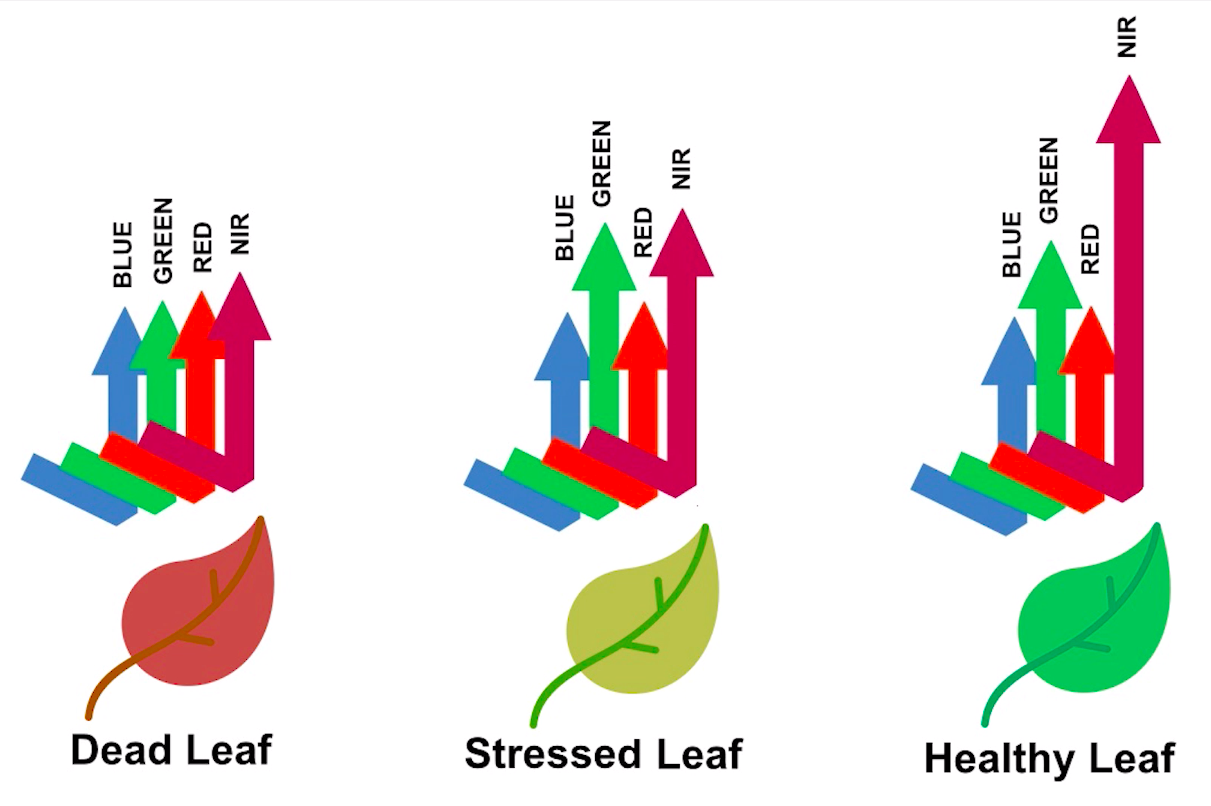
\includegraphics[keepaspectratio]{img/earth-analytics/remote-sensing/spectral_vegetation_stress.png}}
\textgreater{} Image source:
\href{https://github.com/px39n/Awesome-Vegetation-Index}{Spectral
signature literature review by px39n}

Different species of plants reflect different spectral signatures, but
the \emph{pattern} of the signatures across species and sitations is
similar. NDVI compares the amount of NIR reflectance to the amount of
Red reflectance, thus accounting for many of the species differences and
isolating the health of the plant. The formula for calculating NDVI is:

\[NDVI = \frac{(NIR - Red)}{(NIR + Red)}\]

\begin{tcolorbox}[enhanced jigsaw, colbacktitle=quarto-callout-color!10!white, opacityback=0, bottomtitle=1mm, toptitle=1mm, bottomrule=.15mm, left=2mm, colframe=quarto-callout-color-frame, leftrule=.75mm, opacitybacktitle=0.6, colback=white, rightrule=.15mm, toprule=.15mm, breakable, titlerule=0mm, title=\textcolor{quarto-callout-color}{\faInfo}\hspace{0.5em}{Read More}, coltitle=black, arc=.35mm]

Read more about NDVI and other vegetation indices:

\begin{itemize}
\tightlist
\item
  \href{https://www.earthdatascience.org/courses/use-data-open-source-python/multispectral-remote-sensing/vegetation-indices-in-python/calculate-NDVI-python/}{earthdatascience.org}
\item
  \href{https://www.usgs.gov/landsat-missions/landsat-surface-reflectance-derived-spectral-indices}{USGS}
\end{itemize}

\end{tcolorbox}

\subsection{Earth Data Science data
formats}\label{earth-data-science-data-formats}

In Earth Data Science, we get data in three main formats:

\begin{longtable}[]{@{}
  >{\raggedright\arraybackslash}p{(\linewidth - 6\tabcolsep) * \real{0.2500}}
  >{\raggedright\arraybackslash}p{(\linewidth - 6\tabcolsep) * \real{0.2500}}
  >{\raggedright\arraybackslash}p{(\linewidth - 6\tabcolsep) * \real{0.2500}}
  >{\raggedright\arraybackslash}p{(\linewidth - 6\tabcolsep) * \real{0.2500}}@{}}
\toprule\noalign{}
\begin{minipage}[b]{\linewidth}\raggedright
Data type
\end{minipage} & \begin{minipage}[b]{\linewidth}\raggedright
Descriptions
\end{minipage} & \begin{minipage}[b]{\linewidth}\raggedright
Common file formats
\end{minipage} & \begin{minipage}[b]{\linewidth}\raggedright
Python type
\end{minipage} \\
\midrule\noalign{}
\endhead
\bottomrule\noalign{}
\endlastfoot
Time Series & The same data points (e.g.~streamflow) collected multiple
times over time & Tabular formats (e.g.~.csv, or .xlsx) & pandas
DataFrame \\
Vector & Points, lines, and areas (with coordinates) & Shapefile (often
an archive like a \texttt{.zip} file because a Shapefile is actually a
collection of at least 3 files) & geopandas GeoDataFrame \\
Raster & Evenly spaced spatial grid (with coordinates) & GeoTIFF
(\texttt{.tif}), NetCDF (\texttt{.nc}), HDF (\texttt{.hdf}) & rioxarray
DataArray \\
\end{longtable}

\begin{tcolorbox}[enhanced jigsaw, colbacktitle=quarto-callout-color!10!white, opacityback=0, bottomtitle=1mm, toptitle=1mm, bottomrule=.15mm, left=2mm, colframe=quarto-callout-color-frame, leftrule=.75mm, opacitybacktitle=0.6, colback=white, rightrule=.15mm, toprule=.15mm, breakable, titlerule=0mm, title=\textcolor{quarto-callout-color}{\faInfo}\hspace{0.5em}{Read More}, coltitle=black, arc=.35mm]

Check out the sections about about
\href{https://www.earthdatascience.org/courses/use-data-open-source-python/intro-vector-data-python/spatial-data-vector-shapefiles/}{vector
data} and
\href{https://www.earthdatascience.org/courses/intro-to-earth-data-science/file-formats/use-spatial-data/use-raster-data/}{raster
data} in the textbook.

\end{tcolorbox}

\bookmarksetup{startatroot}

\chapter{STEP 0: Set up}\label{step-0-set-up-2}

First, you can use the following parameters to change things about the
workflow:

\begin{Shaded}
\begin{Highlighting}[]
\BuiltInTok{id} \OperatorTok{=} \StringTok{\textquotesingle{}shortcourse\textquotesingle{}}
\NormalTok{site\_name }\OperatorTok{=} \StringTok{\textquotesingle{}Tubarjal Valley Saudi Arabia\textquotesingle{}}
\NormalTok{project\_name }\OperatorTok{=} \StringTok{\textquotesingle{}Tubarjal Valley Saudi Arabia Irrigation\textquotesingle{}}
\NormalTok{boundary\_dir }\OperatorTok{=} \StringTok{\textquotesingle{}tubarjal{-}valley\textquotesingle{}}
\NormalTok{event }\OperatorTok{=} \StringTok{\textquotesingle{}groundwater irrigation\textquotesingle{}}
\NormalTok{start\_year }\OperatorTok{=} \StringTok{\textquotesingle{}2001\textquotesingle{}}
\NormalTok{end\_year }\OperatorTok{=} \StringTok{\textquotesingle{}2022\textquotesingle{}}
\NormalTok{event\_year }\OperatorTok{=} \StringTok{\textquotesingle{}2012\textquotesingle{}}
\end{Highlighting}
\end{Shaded}

\section{Import libraries}\label{import-libraries-2}

We'll need some Python libraries to complete this workflow.

\begin{tcolorbox}[enhanced jigsaw, colbacktitle=quarto-callout-color!10!white, opacityback=0, bottomtitle=1mm, toptitle=1mm, bottomrule=.15mm, left=2mm, colframe=quarto-callout-color-frame, leftrule=.75mm, opacitybacktitle=0.6, colback=white, rightrule=.15mm, toprule=.15mm, breakable, titlerule=0mm, title=\textcolor{quarto-callout-color}{\faInfo}\hspace{0.5em}{Try It: Import necessary libraries}, coltitle=black, arc=.35mm]

In the cell below, making sure to keep the packages in order, add
packages for:

\begin{itemize}
\tightlist
\item
  Working with DataFrames
\item
  Working with GeoDataFrames
\item
  Making interactive plots of tabular and vector data
\end{itemize}

\end{tcolorbox}

\begin{tcolorbox}[enhanced jigsaw, colbacktitle=quarto-callout-color!10!white, opacityback=0, bottomtitle=1mm, toptitle=1mm, bottomrule=.15mm, left=2mm, colframe=quarto-callout-color-frame, leftrule=.75mm, opacitybacktitle=0.6, colback=white, rightrule=.15mm, toprule=.15mm, breakable, titlerule=0mm, title=\textcolor{quarto-callout-color}{\faInfo}\hspace{0.5em}{Reflect and Respond}, coltitle=black, arc=.35mm]

What are we using the rest of these packages for? See if you can figure
it out as you complete the notebook.

\end{tcolorbox}

\begin{Shaded}
\begin{Highlighting}[]
\ImportTok{import}\NormalTok{ json}
\ImportTok{from}\NormalTok{ glob }\ImportTok{import}\NormalTok{ glob}

\ImportTok{import}\NormalTok{ earthpy}
\ImportTok{import}\NormalTok{ hvplot.xarray}
\ImportTok{import}\NormalTok{ rioxarray }\ImportTok{as}\NormalTok{ rxr}
\ImportTok{import}\NormalTok{ xarray }\ImportTok{as}\NormalTok{ xr}
\end{Highlighting}
\end{Shaded}

\section{Download sample data}\label{download-sample-data-1}

In this analysis, you'll need to download multiple data files to your
computer rather than streaming them from the web. You'll need to set up
a folder for the files, and while you're at it download the sample data
there.

\begin{tcolorbox}[enhanced jigsaw, colbacktitle=quarto-callout-caution-color!10!white, opacityback=0, bottomtitle=1mm, toptitle=1mm, bottomrule=.15mm, left=2mm, colframe=quarto-callout-caution-color-frame, leftrule=.75mm, opacitybacktitle=0.6, colback=white, rightrule=.15mm, toprule=.15mm, breakable, titlerule=0mm, title={GOTCHA ALERT!}, coltitle=black, arc=.35mm]

A lot of times in Python we say ``directory'' to mean a ``folder'' on
your computer. The two words mean the same thing in this context.

\end{tcolorbox}

\begin{tcolorbox}[enhanced jigsaw, colbacktitle=quarto-callout-color!10!white, opacityback=0, bottomtitle=1mm, toptitle=1mm, bottomrule=.15mm, left=2mm, colframe=quarto-callout-color-frame, leftrule=.75mm, opacitybacktitle=0.6, colback=white, rightrule=.15mm, toprule=.15mm, breakable, titlerule=0mm, title=\textcolor{quarto-callout-color}{\faInfo}\hspace{0.5em}{Try It}, coltitle=black, arc=.35mm]

In the cell below, replace `Project Name' with
`\textbf{?meta:params.project\_name} and 'my-data-folder' with a
\textbf{descriptive} directory name.

\end{tcolorbox}

\begin{Shaded}
\begin{Highlighting}[]
\NormalTok{project }\OperatorTok{=}\NormalTok{ earthpy.Project(}
    \StringTok{\textquotesingle{}Project Name\textquotesingle{}}\NormalTok{, dirname}\OperatorTok{=}\StringTok{\textquotesingle{}my{-}data{-}folder\textquotesingle{}}\NormalTok{)}
\NormalTok{project.get\_data()}
\end{Highlighting}
\end{Shaded}

\bookmarksetup{startatroot}

\chapter{STEP 1: Site map}\label{step-1-site-map-1}

\section{\texorpdfstring{Study Area:
\textbf{?meta:params.site\_name}}{Study Area: ?meta:params.site\_name}}\label{study-area-1}

\begin{tcolorbox}[enhanced jigsaw, colbacktitle=quarto-callout-color!10!white, opacityback=0, bottomtitle=1mm, toptitle=1mm, bottomrule=.15mm, left=2mm, colframe=quarto-callout-color-frame, leftrule=.75mm, opacitybacktitle=0.6, colback=white, rightrule=.15mm, toprule=.15mm, breakable, titlerule=0mm, title=\textcolor{quarto-callout-color}{\faInfo}\hspace{0.5em}{Reflect and Respond}, coltitle=black, arc=.35mm]

For this coding challenge, we are interested in the boundary of the
\textbf{?meta:params.site\_name}, and the health of vegetation in the
area measured on a scale from -1 to 1. In the cell below, answer the
following question: \textbf{What data type do you think the boundary
will be? What about the vegetation health?}

\end{tcolorbox}

\subsection{\texorpdfstring{Load the \textbf{?meta:params.site\_name}
boundary}{Load the ?meta:params.site\_name boundary}}\label{load-the-boundary-1}

\begin{tcolorbox}[enhanced jigsaw, colbacktitle=quarto-callout-color!10!white, opacityback=0, bottomtitle=1mm, toptitle=1mm, bottomrule=.15mm, left=2mm, colframe=quarto-callout-color-frame, leftrule=.75mm, opacitybacktitle=0.6, colback=white, rightrule=.15mm, toprule=.15mm, breakable, titlerule=0mm, title=\textcolor{quarto-callout-color}{\faInfo}\hspace{0.5em}{Try It}, coltitle=black, arc=.35mm]

\begin{itemize}
\tightlist
\item
  Locate the boundary files in your download directory
\item
  Change \texttt{\textquotesingle{}boundary-directory\textquotesingle{}}
  to the actual location
\item
  Load the data into Python and check that it worked
\end{itemize}

\end{tcolorbox}

\begin{Shaded}
\begin{Highlighting}[]
\CommentTok{\# Load in the boundary data}
\NormalTok{boundary\_gdf }\OperatorTok{=}\NormalTok{ gpd.read\_file(}
\NormalTok{    project.project\_dir }\OperatorTok{/} \StringTok{\textquotesingle{}boundary{-}directory\textquotesingle{}}\NormalTok{)}
\CommentTok{\# Check that it worked}
\end{Highlighting}
\end{Shaded}

\begin{Shaded}
\begin{Highlighting}[]
\CommentTok{\# Plot the results with web tile images}
\NormalTok{boundary\_gdf.hvplot()}
\end{Highlighting}
\end{Shaded}

\bookmarksetup{startatroot}

\chapter{STEP 2: Wrangle Raster
Data}\label{step-2-wrangle-raster-data-1}

\section{Load in NDVI data}\label{load-in-ndvi-data-1}

Now you need to load all the downloaded files into Python. Let's start
by getting all the file names. You will also need to extract the date
from the filename. Check out
\href{https://www.earthdatascience.org/courses/intro-to-earth-data-science/write-efficient-python-code/loops/data-workflows-with-loops/}{the
lesson on getting information from filenames in the textbook}.

Instead of writing out the names of all the files you want, you can use
the \texttt{glob} utility to find all files that match a
\textbf{pattern} formed with the \textbf{wildcard} character \texttt{*}.
The wildcard can represent any string of alphanumeric characters. For
example, the pattern
\texttt{\textquotesingle{}file\_*.tif\textquotesingle{}} will match the
files \texttt{\textquotesingle{}file\_1.tif\textquotesingle{}},
\texttt{\textquotesingle{}file\_2.tiv\textquotesingle{}}, or even
\texttt{\textquotesingle{}file\_qeoiurghtfoqaegbn34pf.tif\textquotesingle{}}\ldots{}
but it will not match
\texttt{\textquotesingle{}something-else.csv\textquotesingle{}} or even
\texttt{\textquotesingle{}something-else.tif\textquotesingle{}}.

In this notebook, we'll use the \texttt{.rglob()}, or \textbf{recursive}
glob method of the Path object instead. It works similarly, but you'll
notice that we have to convert the results to a list with the
\texttt{list()} function.

\begin{tcolorbox}[enhanced jigsaw, colbacktitle=quarto-callout-caution-color!10!white, opacityback=0, bottomtitle=1mm, toptitle=1mm, bottomrule=.15mm, left=2mm, colframe=quarto-callout-caution-color-frame, leftrule=.75mm, opacitybacktitle=0.6, colback=white, rightrule=.15mm, toprule=.15mm, breakable, titlerule=0mm, title=\textcolor{quarto-callout-caution-color}{\faFire}\hspace{0.5em}{GOTCHA ALERT!}, coltitle=black, arc=.35mm]

\texttt{glob} doesn't necessarily find files in the order you would
expect. Make sure to \textbf{sort} your file names like it says in the
textbook.

\end{tcolorbox}

\begin{tcolorbox}[enhanced jigsaw, colbacktitle=quarto-callout-color!10!white, opacityback=0, bottomtitle=1mm, toptitle=1mm, bottomrule=.15mm, left=2mm, colframe=quarto-callout-color-frame, leftrule=.75mm, opacitybacktitle=0.6, colback=white, rightrule=.15mm, toprule=.15mm, breakable, titlerule=0mm, title=\textcolor{quarto-callout-color}{\faInfo}\hspace{0.5em}{Reflect and Respond}, coltitle=black, arc=.35mm]

Take a look at the file names for the NDVI files. What do you notice is
the same for all the files? Keep in mind that for this analysis you only
want to import the NDVI files, not the Quality files (which would be
used to identify potential incorrect measurements).

\end{tcolorbox}

\begin{tcolorbox}[enhanced jigsaw, colbacktitle=quarto-callout-color!10!white, opacityback=0, bottomtitle=1mm, toptitle=1mm, bottomrule=.15mm, left=2mm, colframe=quarto-callout-color-frame, leftrule=.75mm, opacitybacktitle=0.6, colback=white, rightrule=.15mm, toprule=.15mm, breakable, titlerule=0mm, title=\textcolor{quarto-callout-color}{\faInfo}\hspace{0.5em}{Try It}, coltitle=black, arc=.35mm]

\begin{enumerate}
\def\labelenumi{\arabic{enumi}.}
\tightlist
\item
  Create a \textbf{pattern} for the files you want to import. Your
  pattern should include the parts of the file names that are the same
  for all files, and replace the rest with the \texttt{*} character.
  Make sure to match the NDVI files, but not the Quality files!
\item
  Replace \texttt{ndvi-pattern} with your pattern
\item
  Run the code and make sure that you are getting all the files you want
  and none of the files you don't!
\end{enumerate}

\end{tcolorbox}

\begin{Shaded}
\begin{Highlighting}[]
\CommentTok{\# Get a sorted list of NDVI tif file paths}
\NormalTok{ndvi\_paths }\OperatorTok{=} \BuiltInTok{sorted}\NormalTok{(}\BuiltInTok{list}\NormalTok{(project.project\_dir.rglob(}\StringTok{\textquotesingle{}ndvi{-}pattern\textquotesingle{}}\NormalTok{)))}

\CommentTok{\# Display the first and last three files paths to check the pattern}
\NormalTok{ndvi\_paths[:}\DecValTok{3}\NormalTok{], ndvi\_paths[}\OperatorTok{{-}}\DecValTok{3}\NormalTok{:]}
\end{Highlighting}
\end{Shaded}

\section{Repeating tasks in Python}\label{repeating-tasks-in-python-2}

Now you should have a few dozen files! For each file, you need to:

\begin{itemize}
\tightlist
\item
  Load the file in using the \texttt{rioxarray} library
\item
  Get the date from the file name
\item
  Add the date as a dimension coordinate
\item
  Give your data variable a name
\end{itemize}

You don't want to write out the code for each file! That's a recipe for
copy pasta. Luckily, Python has tools for doing similar tasks
repeatedly. In this case, you'll use one called a \texttt{for} loop.

There's some code below that uses a \texttt{for} loop in what is called
an \textbf{accumulation pattern} to process each file. That means that
you will save the results of your processing to a list each time you
process the files, and then merge all the arrays in the list.

\begin{tcolorbox}[enhanced jigsaw, colbacktitle=quarto-callout-color!10!white, opacityback=0, bottomtitle=1mm, toptitle=1mm, bottomrule=.15mm, left=2mm, colframe=quarto-callout-color-frame, leftrule=.75mm, opacitybacktitle=0.6, colback=white, rightrule=.15mm, toprule=.15mm, breakable, titlerule=0mm, title=\textcolor{quarto-callout-color}{\faInfo}\hspace{0.5em}{Try It}, coltitle=black, arc=.35mm]

\begin{itemize}
\tightlist
\item
  Look at the file names. How many characters from the end is the date?
  \texttt{doy\_start} and \texttt{doy\_end} are used to extract the day
  of the year (doy) from the file name. You will need to count
  characters from the end and change the values to get the right part of
  the file name. HINT: the index -1 in Python means the last value, -2
  second-to-last, and so on.
\item
  Replace any required variable names with your chosen variable names
\end{itemize}

\end{tcolorbox}

\begin{Shaded}
\begin{Highlighting}[]
\NormalTok{doy\_start }\OperatorTok{=} \OperatorTok{{-}}\DecValTok{1}
\NormalTok{doy\_end }\OperatorTok{=} \OperatorTok{{-}}\DecValTok{1}

\CommentTok{\# Loop through each NDVI image}
\NormalTok{ndvi\_das }\OperatorTok{=}\NormalTok{ []}
\ControlFlowTok{for}\NormalTok{ ndvi\_path }\KeywordTok{in}\NormalTok{ ndvi\_paths:}
    \CommentTok{\# Get date from file name}

    \CommentTok{\# Open dataset}

    \CommentTok{\# Add date dimension and clean up metadata}
\NormalTok{    da }\OperatorTok{=}\NormalTok{ da.assign\_coords(\{}\StringTok{\textquotesingle{}date\textquotesingle{}}\NormalTok{: date\})}
\NormalTok{    da }\OperatorTok{=}\NormalTok{ da.expand\_dims(\{}\StringTok{\textquotesingle{}date\textquotesingle{}}\NormalTok{: }\DecValTok{1}\NormalTok{\})}
\NormalTok{    da.name }\OperatorTok{=} \StringTok{\textquotesingle{}NDVI\textquotesingle{}}

    \CommentTok{\# Prepare for concatenation}
\end{Highlighting}
\end{Shaded}

\section{Combine Rasters}\label{combine-rasters-1}

Next, stack your arrays by date into a time series using the
\texttt{xr.combine\_by\_coords()} function. You will have to tell it
which dimension you want to stack your data in.

\begin{Shaded}
\begin{Highlighting}[]
\CommentTok{\# Combine NDVI images from all dates}
\end{Highlighting}
\end{Shaded}

\bookmarksetup{startatroot}

\chapter{STEP 3: Plot NDVI}\label{step-3-plot-ndvi-1}

\begin{tcolorbox}[enhanced jigsaw, colbacktitle=quarto-callout-color!10!white, opacityback=0, bottomtitle=1mm, toptitle=1mm, bottomrule=.15mm, left=2mm, colframe=quarto-callout-color-frame, leftrule=.75mm, opacitybacktitle=0.6, colback=white, rightrule=.15mm, toprule=.15mm, breakable, titlerule=0mm, title=\textcolor{quarto-callout-color}{\faInfo}\hspace{0.5em}{Try It: Plot the change in NDVI spatially}, coltitle=black, arc=.35mm]

Complete the following:

\begin{itemize}
\tightlist
\item
  Select data from before the \textbf{?meta:params.event}
  (\textbf{?meta:params.start\_year} to
  \textbf{?meta:params.event\_year})
\item
  Take the temporal mean (over the \textbf{date}, not spatially)
\item
  Get the NDVI variable (should be a DataArray, not a Dataset)
\item
  Repeat for the data from after the \textbf{?meta:params.event}
  (\textbf{?meta:params.event\_year} to \textbf{?meta:params.end\_year})
\item
  Subtract the pre-event data \textbf{from} the post-event data
\item
  Plot the result using a \textbf{diverging} color map like
  \texttt{cmap=plt.cm.PiYG}
\end{itemize}

There are different types of color maps for different types of data. In
this case, we want decreases to be a different color from increases, so
we should use a \textbf{diverging} color map. Check out available
colormaps in the
\href{https://matplotlib.org/stable/tutorials/colors/colormaps.html}{matplotlib
documentation}.

\end{tcolorbox}

\begin{tcolorbox}[enhanced jigsaw, colbacktitle=quarto-callout-color!10!white, opacityback=0, bottomtitle=1mm, toptitle=1mm, bottomrule=.15mm, left=2mm, colframe=quarto-callout-color-frame, leftrule=.75mm, opacitybacktitle=0.6, colback=white, rightrule=.15mm, toprule=.15mm, breakable, titlerule=0mm, title=\textcolor{quarto-callout-color}{\faInfo}\hspace{0.5em}{Looking for an Extra Challenge?}, coltitle=black, arc=.35mm]

For an extra challenge, add the \textbf{?meta:params.site\_name}
boundary to the plot.

\end{tcolorbox}

\begin{Shaded}
\begin{Highlighting}[]
\CommentTok{\# Compute the difference in NDVI before and after}

\CommentTok{\# Plot the difference}
\NormalTok{(}
\NormalTok{    ndvi\_diff.hvplot(x}\OperatorTok{=}\StringTok{\textquotesingle{}\textquotesingle{}}\NormalTok{, y}\OperatorTok{=}\StringTok{\textquotesingle{}\textquotesingle{}}\NormalTok{, cmap}\OperatorTok{=}\StringTok{\textquotesingle{}\textquotesingle{}}\NormalTok{, geo}\OperatorTok{=}\VariableTok{True}\NormalTok{)}
    \OperatorTok{*}
\NormalTok{    gdf.hvplot(geo}\OperatorTok{=}\VariableTok{True}\NormalTok{, fill\_color}\OperatorTok{=}\VariableTok{None}\NormalTok{, line\_color}\OperatorTok{=}\StringTok{\textquotesingle{}black\textquotesingle{}}\NormalTok{)}
\NormalTok{)}
\end{Highlighting}
\end{Shaded}

\bookmarksetup{startatroot}

\chapter{\texorpdfstring{STEP 4: Is the NDVI different after the
\textbf{?meta:params.event}?}{STEP 4: Is the NDVI different after the ?meta:params.event?}}\label{step-4-is-the-ndvi-different-after-the}

You will apply an NDVI threshold and determine how many pixels have
healthy vegetation. You can then look at the growth of vegetation over
time.

\begin{tcolorbox}[enhanced jigsaw, colbacktitle=quarto-callout-color!10!white, opacityback=0, bottomtitle=1mm, toptitle=1mm, bottomrule=.15mm, left=2mm, colframe=quarto-callout-color-frame, leftrule=.75mm, opacitybacktitle=0.6, colback=white, rightrule=.15mm, toprule=.15mm, breakable, titlerule=0mm, title=\textcolor{quarto-callout-color}{\faInfo}\hspace{0.5em}{Try It}, coltitle=black, arc=.35mm]

\begin{itemize}
\tightlist
\item
  Apply an NDVI threshold to identify pixels with healthy vegetation
\item
  Check that your threshold worked
\end{itemize}

\end{tcolorbox}

\begin{Shaded}
\begin{Highlighting}[]
\CommentTok{\# Apply NDVI threshold}
\end{Highlighting}
\end{Shaded}

Now, add up the number of pixels with healthy vegetation plot that over
time.

\begin{Shaded}
\begin{Highlighting}[]
\CommentTok{\# Plot difference inside and outside the boundary}
\end{Highlighting}
\end{Shaded}

Finally, plot your \texttt{DataFrame}. What do you observe? Don't forget
to write a headline and description of your plot!

\begin{Shaded}
\begin{Highlighting}[]
\CommentTok{\# Plot number of vegetated pixels over time}
\end{Highlighting}
\end{Shaded}

\bookmarksetup{startatroot}

\chapter{Vegetation Data Access}\label{vegetation-data-access-1}

Accessing NDVI data

\hfill\break

\bookmarksetup{startatroot}

\chapter{STEP 0: Set up}\label{step-0-set-up-3}

\section{Import libraries}\label{import-libraries-3}

We'll need some Python libraries to complete this workflow.

\begin{tcolorbox}[enhanced jigsaw, colbacktitle=quarto-callout-color!10!white, opacityback=0, bottomtitle=1mm, toptitle=1mm, bottomrule=.15mm, left=2mm, colframe=quarto-callout-color-frame, leftrule=.75mm, opacitybacktitle=0.6, colback=white, rightrule=.15mm, toprule=.15mm, breakable, titlerule=0mm, title=\textcolor{quarto-callout-color}{\faInfo}\hspace{0.5em}{Try It: Import necessary libraries}, coltitle=black, arc=.35mm]

In the cell below, making sure to keep the packages in order, add
packages for:

\begin{itemize}
\tightlist
\item
  Working with DataFrames
\item
  Working with GeoDataFrames
\item
  Making interactive plots of tabular and vector data
\end{itemize}

\end{tcolorbox}

\begin{tcolorbox}[enhanced jigsaw, colbacktitle=quarto-callout-color!10!white, opacityback=0, bottomtitle=1mm, toptitle=1mm, bottomrule=.15mm, left=2mm, colframe=quarto-callout-color-frame, leftrule=.75mm, opacitybacktitle=0.6, colback=white, rightrule=.15mm, toprule=.15mm, breakable, titlerule=0mm, title=\textcolor{quarto-callout-color}{\faInfo}\hspace{0.5em}{Reflect and Respond}, coltitle=black, arc=.35mm]

What are we using the rest of these packages for? See if you can figure
it out as you complete the notebook.

\end{tcolorbox}

\begin{Shaded}
\begin{Highlighting}[]
\ImportTok{import}\NormalTok{ json}
\ImportTok{import}\NormalTok{ os}
\ImportTok{import}\NormalTok{ pathlib}
\ImportTok{import}\NormalTok{ shutil}
\ImportTok{from}\NormalTok{ glob }\ImportTok{import}\NormalTok{ glob}

\ImportTok{import}\NormalTok{ earthpy.api.appeears }\ImportTok{as}\NormalTok{ eaapp}
\ImportTok{import}\NormalTok{ earthpy}
\ImportTok{import}\NormalTok{ hvplot.xarray}
\ImportTok{import}\NormalTok{ rioxarray }\ImportTok{as}\NormalTok{ rxr}
\ImportTok{import}\NormalTok{ xarray }\ImportTok{as}\NormalTok{ xr}
\end{Highlighting}
\end{Shaded}

Next, we'll set some parameters that are used later on in the workflow.
You can use these to customize your workflow, or you can choose to put
the values you want directly into your code.

\begin{Shaded}
\begin{Highlighting}[]
\BuiltInTok{id} \OperatorTok{=} \StringTok{\textquotesingle{}shortcourse\textquotesingle{}}
\NormalTok{data\_dir }\OperatorTok{=} \StringTok{\textquotesingle{}tubarjal\textquotesingle{}}
\NormalTok{download\_key }\OperatorTok{=} \StringTok{\textquotesingle{}tubarjal{-}ndvi\textquotesingle{}}
\NormalTok{project\_title }\OperatorTok{=} \StringTok{\textquotesingle{}Irrigation in Saudi Arabia\textquotesingle{}}
\NormalTok{start\_year }\OperatorTok{=} \DecValTok{2001}
\NormalTok{end\_year }\OperatorTok{=} \DecValTok{2022}
\NormalTok{event\_year }\OperatorTok{=} \DecValTok{2012}
\NormalTok{address }\OperatorTok{=} \StringTok{\textquotesingle{}Wadi Tubarjal\textquotesingle{}}
\NormalTok{tag\_key }\OperatorTok{=} \StringTok{\textquotesingle{}natural\textquotesingle{}}
\NormalTok{tag\_value }\OperatorTok{=} \StringTok{\textquotesingle{}valley\textquotesingle{}}
\NormalTok{boundary\_dirname }\OperatorTok{=} \StringTok{\textquotesingle{}tubarjal{-}valley\textquotesingle{}}
\end{Highlighting}
\end{Shaded}

We have one more setup task. We're not going to be able to load all our
data directly from the web to Python this time. That means we need to
set up a place for it.

\begin{tcolorbox}[enhanced jigsaw, colbacktitle=quarto-callout-caution-color!10!white, opacityback=0, bottomtitle=1mm, toptitle=1mm, bottomrule=.15mm, left=2mm, colframe=quarto-callout-caution-color-frame, leftrule=.75mm, opacitybacktitle=0.6, colback=white, rightrule=.15mm, toprule=.15mm, breakable, titlerule=0mm, title={GOTCHA ALERT!}, coltitle=black, arc=.35mm]

A lot of times in Python we say ``directory'' to mean a ``folder'' on
your computer. The two words mean the same thing in this context.

\end{tcolorbox}

\begin{tcolorbox}[enhanced jigsaw, colbacktitle=quarto-callout-color!10!white, opacityback=0, bottomtitle=1mm, toptitle=1mm, bottomrule=.15mm, left=2mm, colframe=quarto-callout-color-frame, leftrule=.75mm, opacitybacktitle=0.6, colback=white, rightrule=.15mm, toprule=.15mm, breakable, titlerule=0mm, title=\textcolor{quarto-callout-color}{\faInfo}\hspace{0.5em}{Try It}, coltitle=black, arc=.35mm]

\begin{enumerate}
\def\labelenumi{\arabic{enumi}.}
\tightlist
\item
  Replace `my-data-folder' with a \textbf{descriptive} directory name.
\item
  Run the cell to display your project directory.
\item
  Can you find the directory, either in a terminal or through your
  operating system's file browser/explorer/finder?
\end{enumerate}

\end{tcolorbox}

\begin{Shaded}
\begin{Highlighting}[]
\CommentTok{\# Create a project directory in the system data folder}
\NormalTok{project }\OperatorTok{=}\NormalTok{ earthpy.project.Project(}
\NormalTok{    dirname}\OperatorTok{=}\StringTok{\textquotesingle{}my{-}data{-}folder\textquotesingle{}}\NormalTok{)}
\NormalTok{project.project\_dir}
\end{Highlighting}
\end{Shaded}

\bookmarksetup{startatroot}

\chapter{Download Study Area}\label{download-study-area}

You can use any boundary for your study. One great way to get political
boundaries is through the Open Street Map API. Open Street Map is an
open-source, editable map of the world -- a little like a wiki for
places. They also provide a service (or API) for looking up locations
using code.

\section{Search online}\label{search-online}

It can be a little tricky to find the place you want using the OSM API.
We recommend that you start out on the
\href{https://www.openstreetmap.org/}{Open Street Map (OSM)} web page,
and search for your site there. Then, you can get key pieces of
information you will need to reproducibly find your site area using
code.

In this example, we are downloading images to match
\href{https://svs.gsfc.nasa.gov/11290}{these images from NASA}.

\subsection{STEP 1A: Navigate to Open Street
Map}\label{step-1a-navigate-to-open-street-map}

\begin{figure}[H]

{\centering \pandocbounded{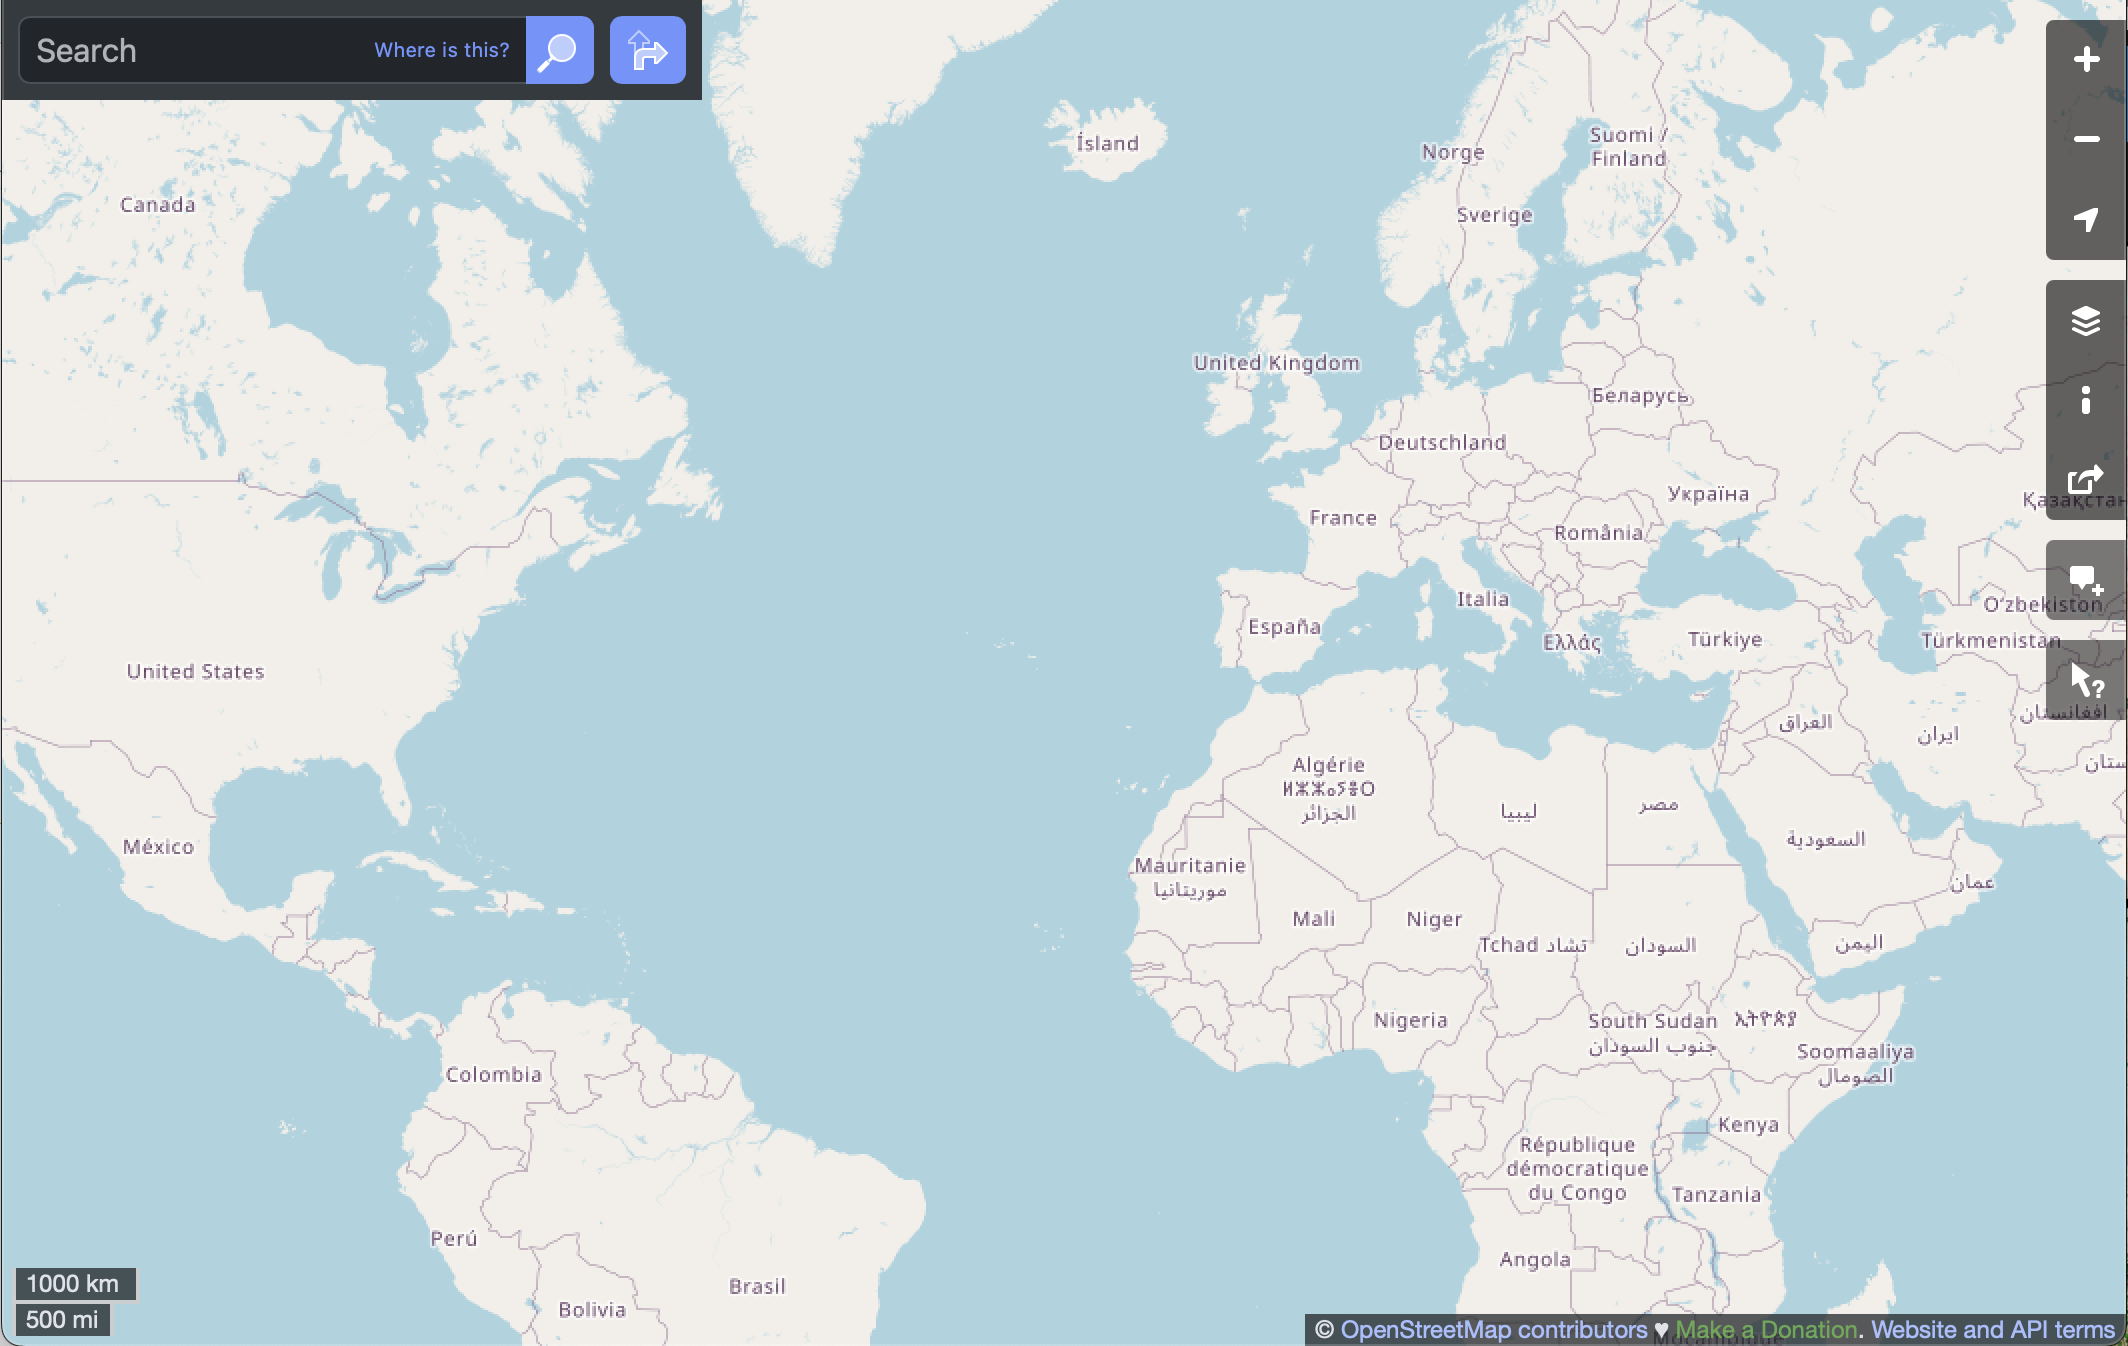
\includegraphics[keepaspectratio]{img/earth-analytics/irrigation/osm-saudi-arabia/00-osm-site.png}}

}

\caption{Start out on the \href{https://www.openstreetmap.org/}{Open
Street Map (OSM)} web page}

\end{figure}%

\subsection{STEP 1B: Search for a nearby
landmark}\label{step-1b-search-for-a-nearby-landmark}

We'll start by searching for the town of Tubarjal.

\begin{figure}[H]

{\centering \pandocbounded{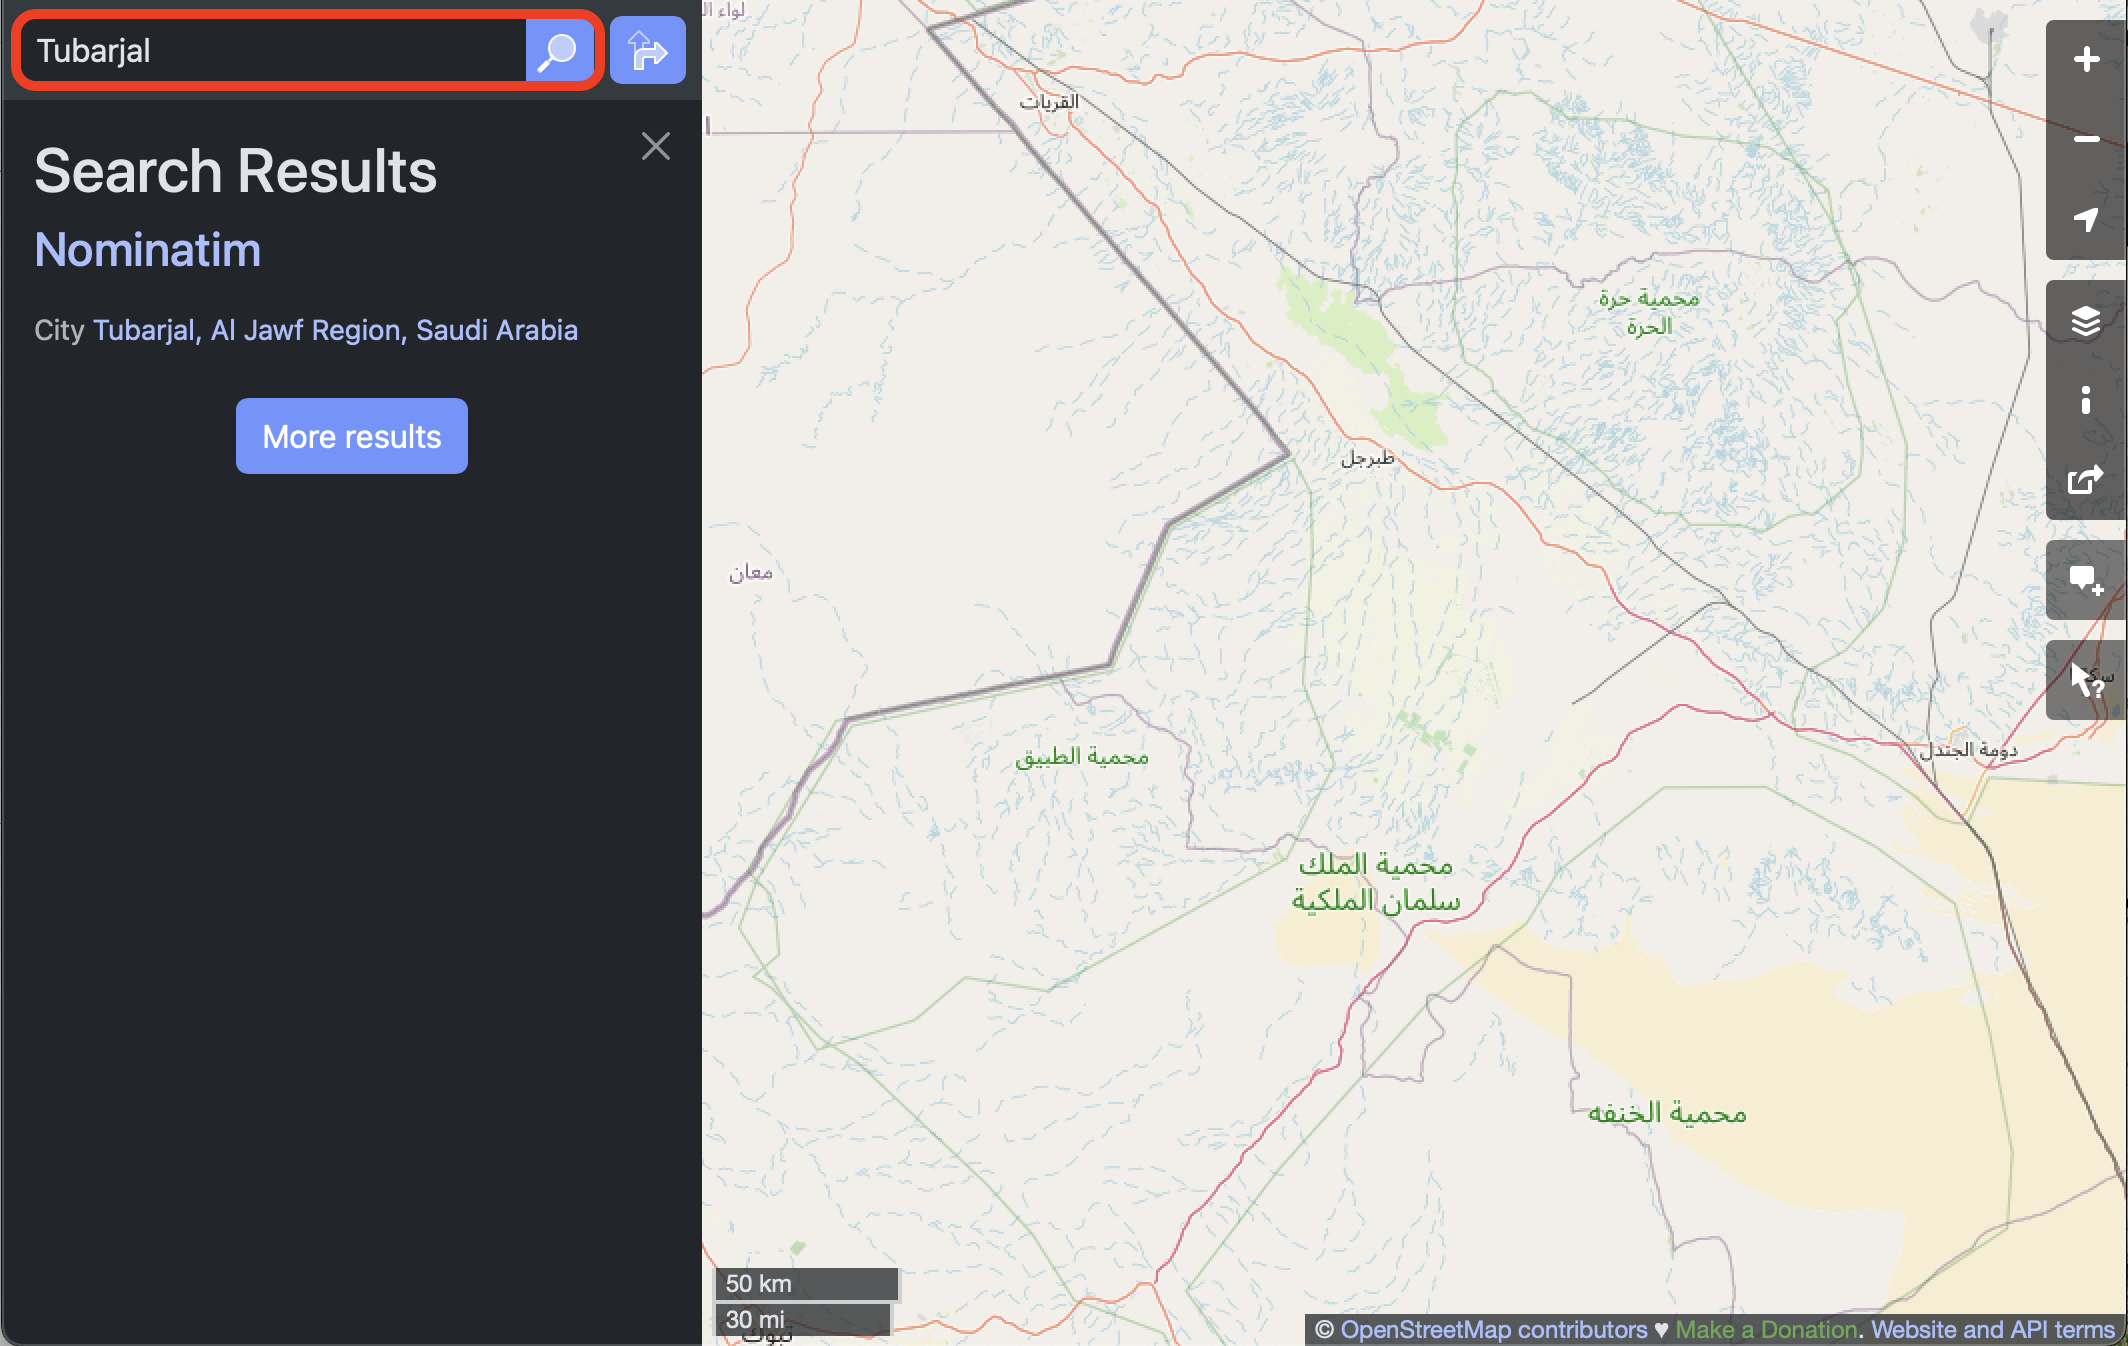
\includegraphics[keepaspectratio]{img/earth-analytics/irrigation/osm-saudi-arabia/01-search-landmark.png}}

}

\caption{Search for Tubarjal.}

\end{figure}%

\begin{figure}[H]

{\centering \pandocbounded{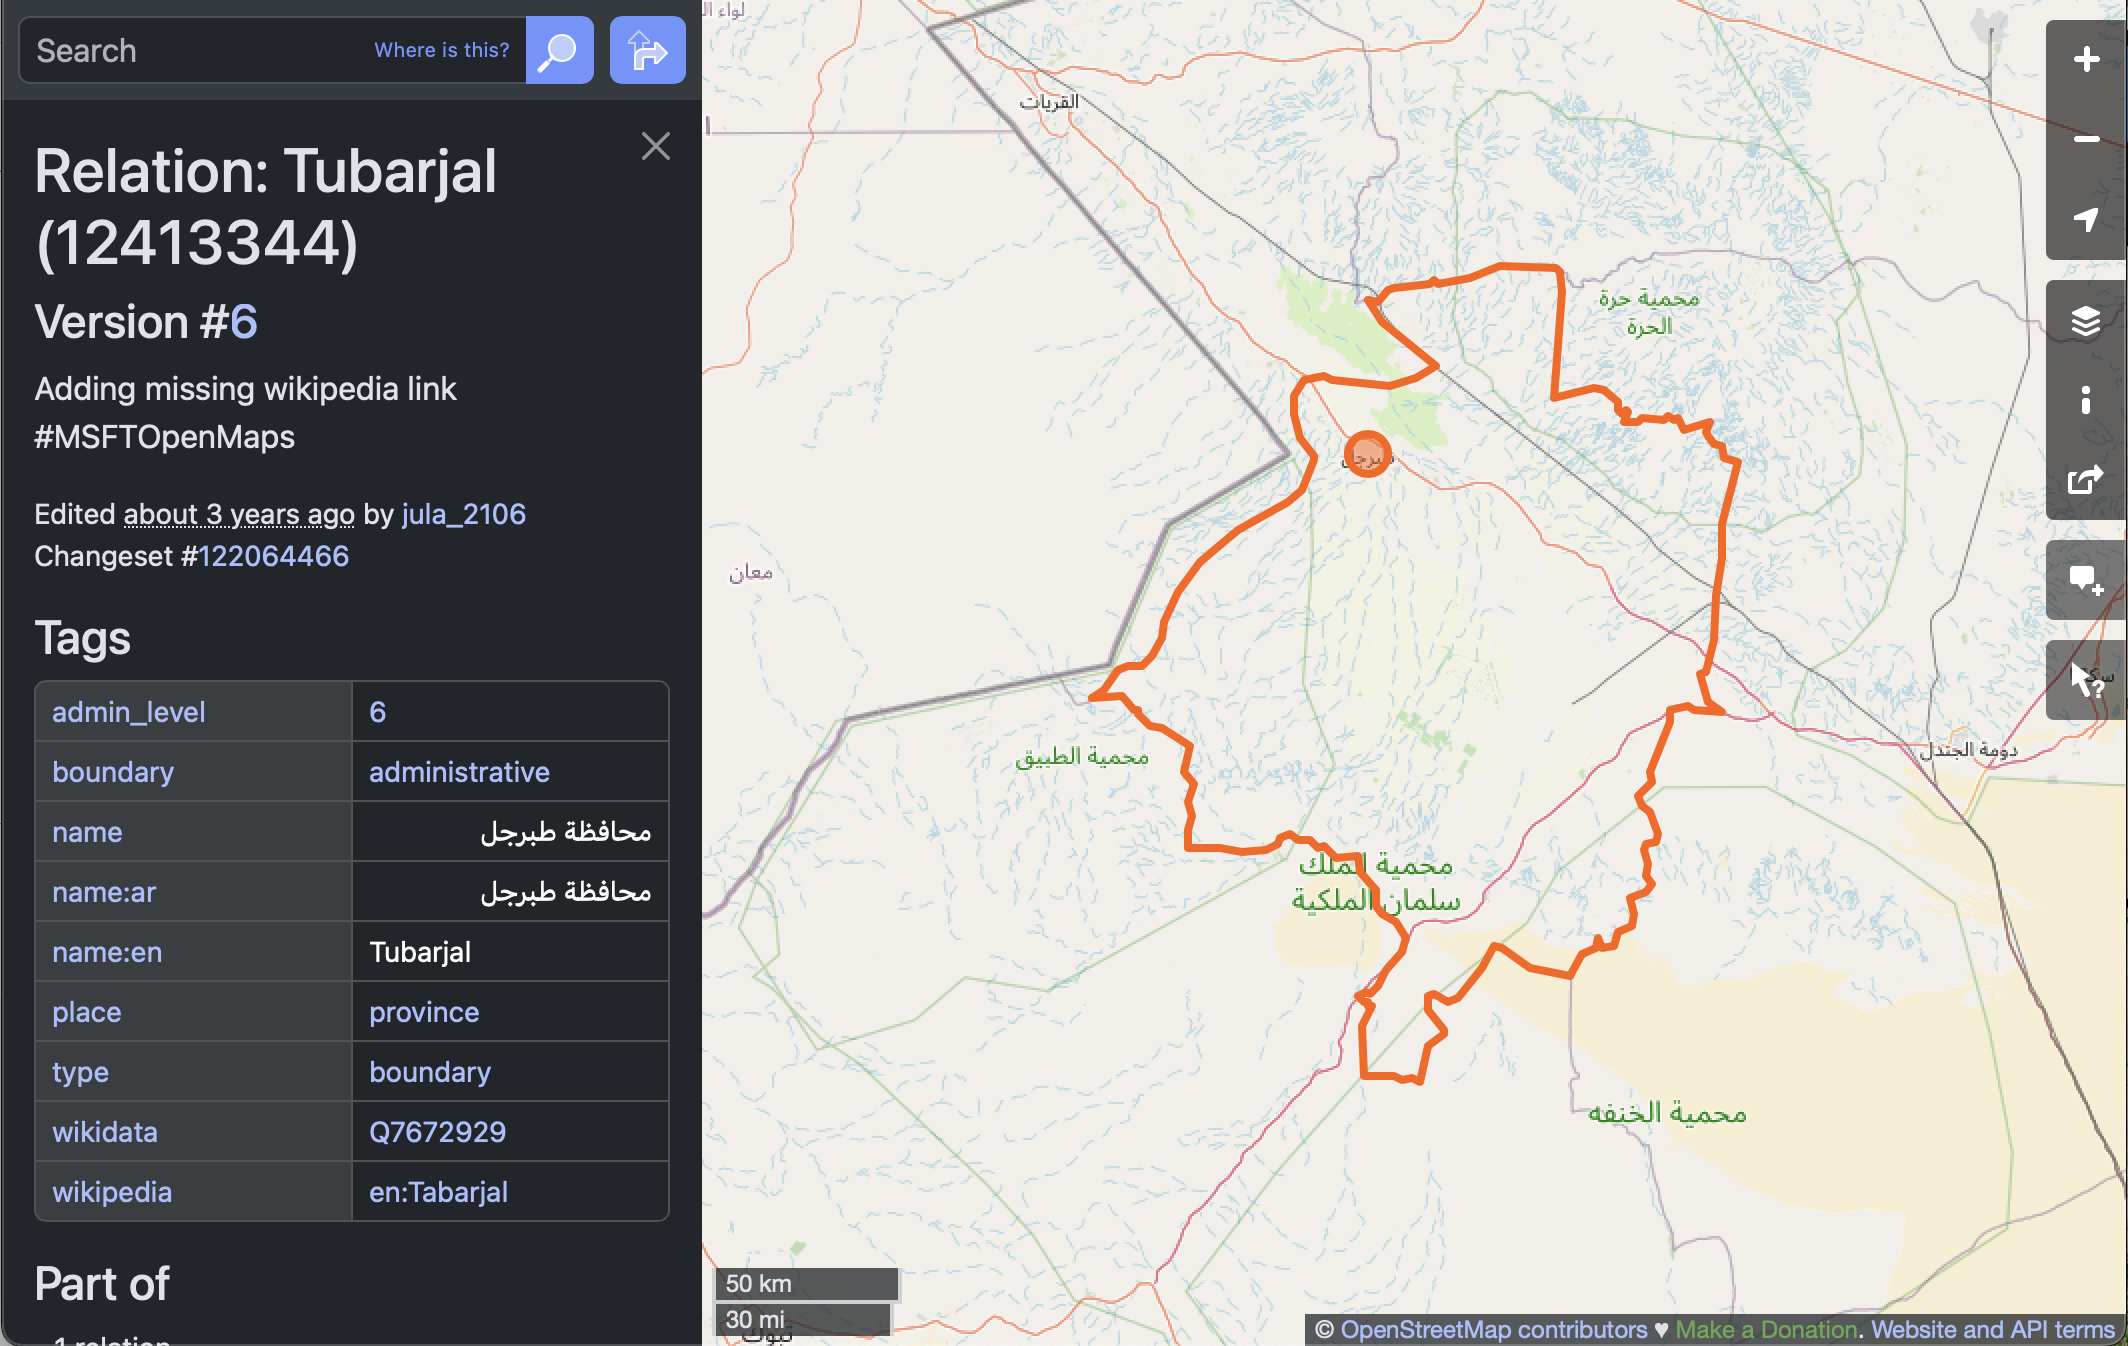
\includegraphics[keepaspectratio]{img/earth-analytics/irrigation/osm-saudi-arabia/02-search-result.png}}

}

\caption{Select the first result.}

\end{figure}%

\subsection{STEP 1C: Select the region}\label{step-1c-select-the-region}

We'll need and area, not just a point, as a site boundary.

\pandocbounded{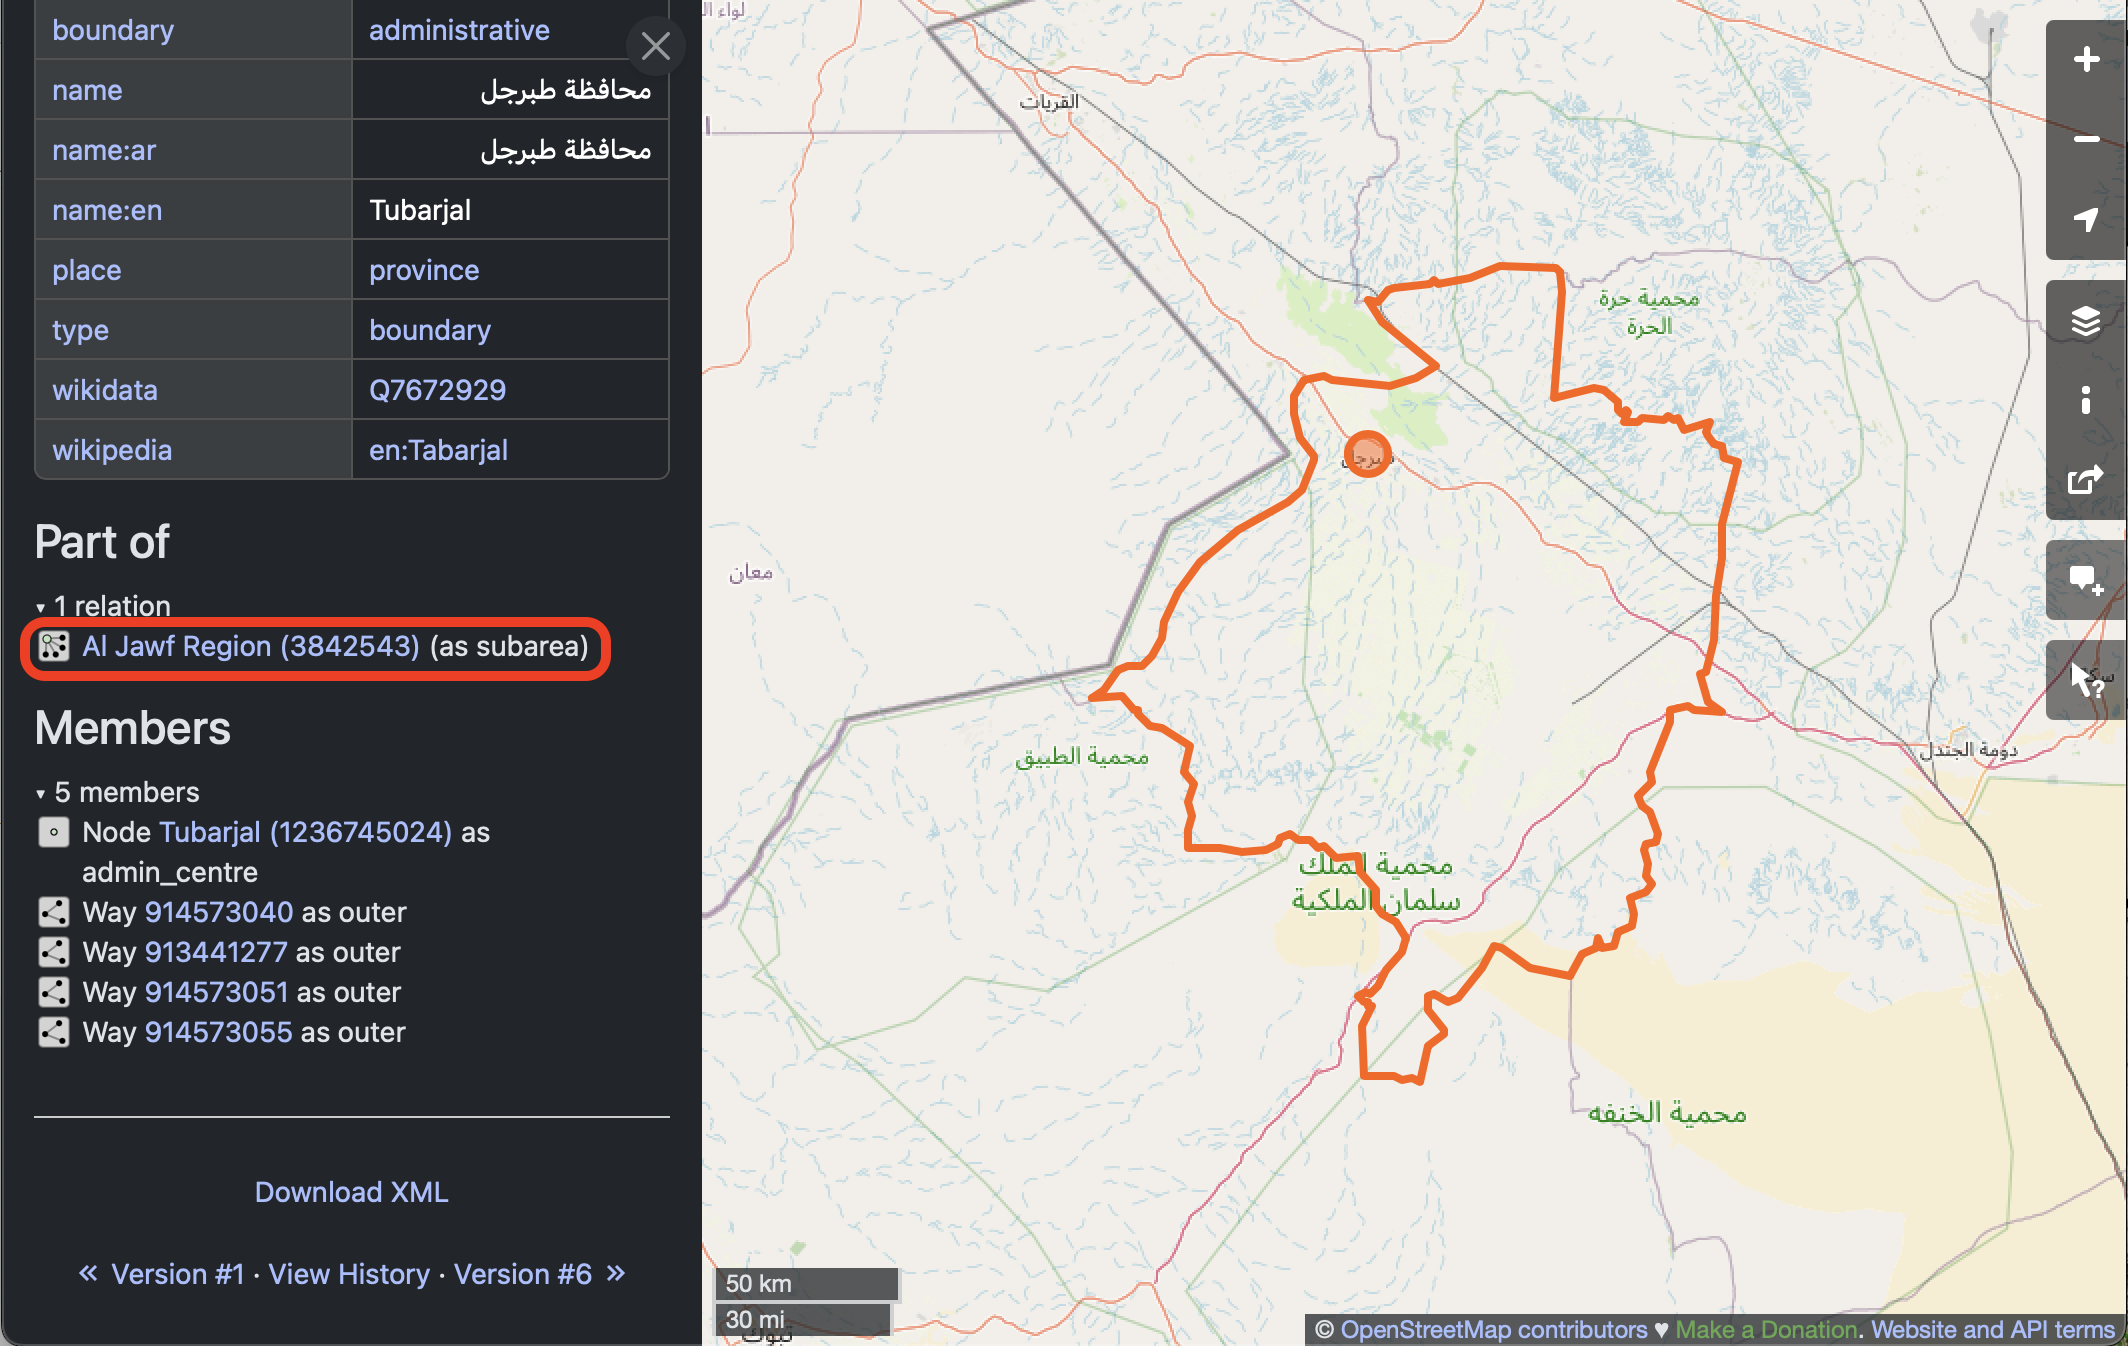
\includegraphics[keepaspectratio]{img/earth-analytics/irrigation/osm-saudi-arabia/03-select-region.png}}
Make a note of the name of the region, as well as at least one of the
tags, for later.

\begin{figure}[H]

{\centering \pandocbounded{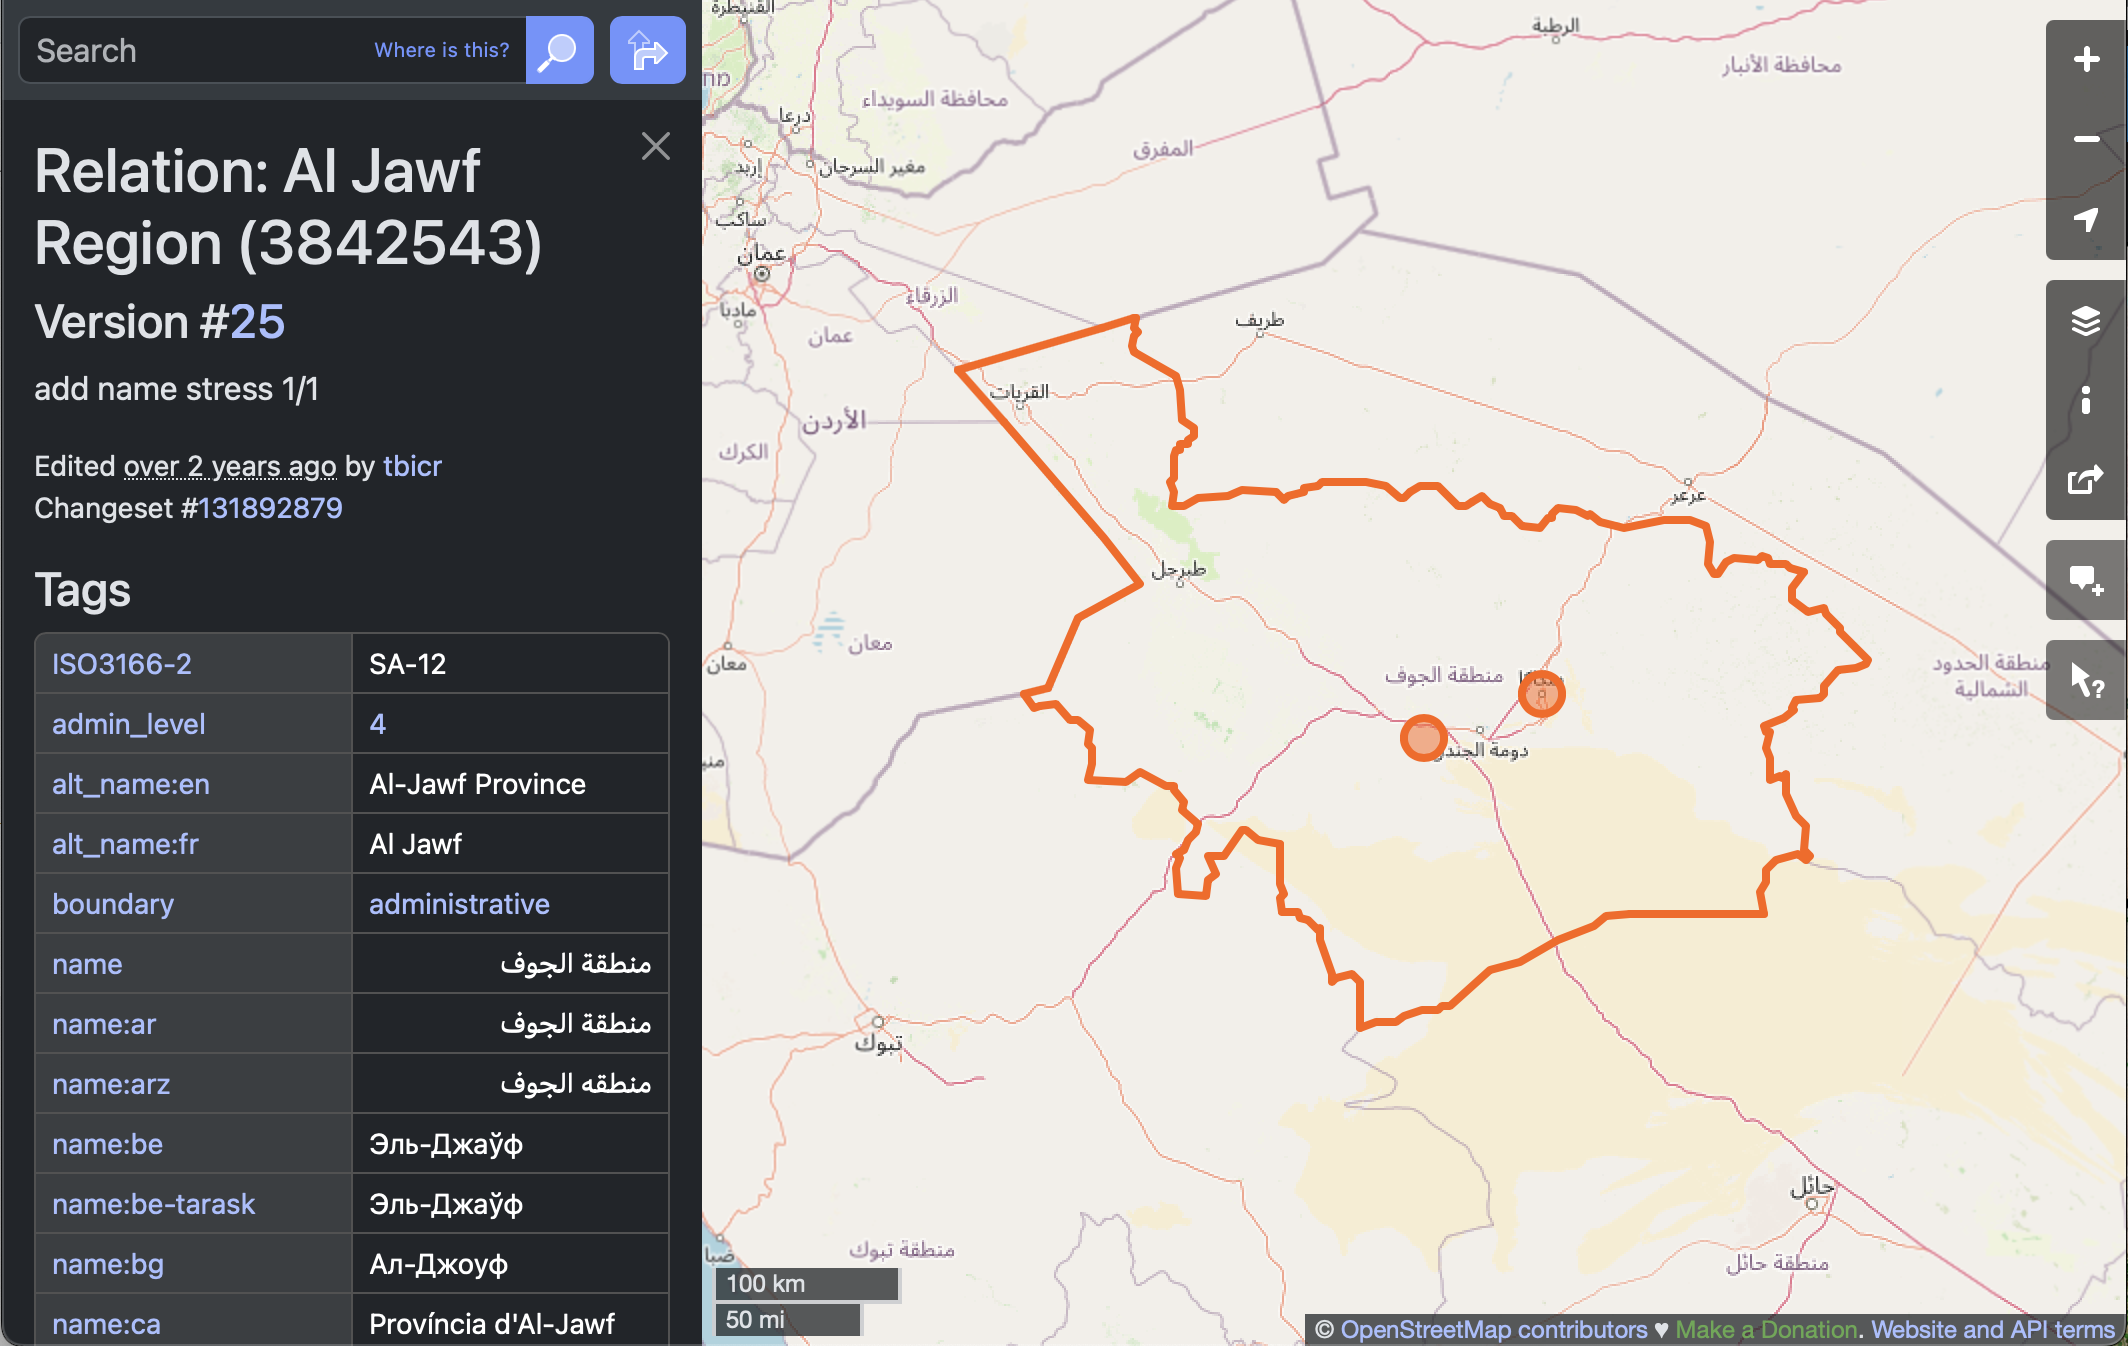
\includegraphics[keepaspectratio]{img/earth-analytics/irrigation/osm-saudi-arabia/04-region-result.png}}

}

\caption{Copy key details about the Al Jawr region from the OSM page.}

\end{figure}%

\bookmarksetup{startatroot}

\chapter{STEP 0: Import Mapping
packages}\label{step-0-import-mapping-packages}

To access the Open Street Map API, we'll use the osmnx package.

\begin{tcolorbox}[enhanced jigsaw, colbacktitle=quarto-callout-color!10!white, opacityback=0, bottomtitle=1mm, toptitle=1mm, bottomrule=.15mm, left=2mm, colframe=quarto-callout-color-frame, leftrule=.75mm, opacitybacktitle=0.6, colback=white, rightrule=.15mm, toprule=.15mm, breakable, titlerule=0mm, title=\textcolor{quarto-callout-color}{\faInfo}\hspace{0.5em}{Try It}, coltitle=black, arc=.35mm]

Add code to import the other necessary libraries to:

\begin{enumerate}
\def\labelenumi{\arabic{enumi}.}
\tightlist
\item
  Create interactive maps and plots
\item
  Save maps and plots to .html files
\end{enumerate}

\end{tcolorbox}

\begin{Shaded}
\begin{Highlighting}[]
\CommentTok{\# Save maps and plots to HTML files}
\CommentTok{\# Create interactive maps and plots}
\ImportTok{from}\NormalTok{ osmnx }\ImportTok{import}\NormalTok{ features }\ImportTok{as}\NormalTok{ osm }\CommentTok{\# Search for locations by name}
\end{Highlighting}
\end{Shaded}

\bookmarksetup{startatroot}

\chapter{STEP 1: Search for a point of
interest}\label{step-1-search-for-a-point-of-interest}

You can use the \texttt{osmnx} package to download and search for
spatial vector data in your area, or anywhere around the world.

In this case, we're looking for the location of the United Tribes
Technical College campus in North Dakota. The address in here,
\texttt{\textquotesingle{}United\ Tribes\ Technical\ College,\ Bismarck,\ ND,\ United\ States\textquotesingle{}},
does not have to be complete or exact, but it should be specific enough
to narrow it down.

\begin{tcolorbox}[enhanced jigsaw, colbacktitle=quarto-callout-tip-color!10!white, opacityback=0, bottomtitle=1mm, toptitle=1mm, bottomrule=.15mm, left=2mm, colframe=quarto-callout-tip-color-frame, leftrule=.75mm, opacitybacktitle=0.6, colback=white, rightrule=.15mm, toprule=.15mm, breakable, titlerule=0mm, title=\textcolor{quarto-callout-tip-color}{\faLightbulb}\hspace{0.5em}{Tip}, coltitle=black, arc=.35mm]

You can use the \href{https://www.openstreetmap.org/}{Open Street Maps}
website to fine-tune your address before you copy it into your code.

\end{tcolorbox}

With the \texttt{osmnx} library, in addition to the address or place
name you are using, you need to supply at least one tag. In this case,
we are specifying that we want it to be tagged as a
\textbf{?meta:params.tag\_key} of type \textbf{?meta:params.tag\_value}.
You might have to try a couple different searches with different
addresses and/or tags to get the address you want, just like if you are
using a map website or app.

\begin{tcolorbox}[enhanced jigsaw, colbacktitle=quarto-callout-tip-color!10!white, opacityback=0, bottomtitle=1mm, toptitle=1mm, bottomrule=.15mm, left=2mm, colframe=quarto-callout-tip-color-frame, leftrule=.75mm, opacitybacktitle=0.6, colback=white, rightrule=.15mm, toprule=.15mm, breakable, titlerule=0mm, title=\textcolor{quarto-callout-tip-color}{\faLightbulb}\hspace{0.5em}{Tip}, coltitle=black, arc=.35mm]

Check out the
\href{https://wiki.openstreetmap.org/wiki/Key:amenity}{list of all the
different amenity types available on Open Street Maps}! Different
amenity types might be different types of vector data, such as a
\textbf{point} location or a building footprint \textbf{polygon}.

\end{tcolorbox}

\begin{Shaded}
\begin{Highlighting}[]
\CommentTok{\# Search for your site}
\NormalTok{boundary\_gdf }\OperatorTok{=}\NormalTok{ osm.features\_from\_address(}
\NormalTok{    address,}
\NormalTok{    \{tag\_key: tag\_value\},}
\NormalTok{    dist}\OperatorTok{=}\DecValTok{1000}\NormalTok{)}
\NormalTok{boundary\_gdf}
\end{Highlighting}
\end{Shaded}

\begin{longtable}[]{@{}lllllllllllll@{}}
\toprule\noalign{}
& & geometry & GNS:dsg\_code & GNS:dsg\_name & GNS:id & int\_name &
intermittent & name & name:ar & name:en & natural & waterway \\
element & id & & & & & & & & & & & \\
\midrule\noalign{}
\endhead
\bottomrule\noalign{}
\endlastfoot
way & 1017205033 & LINESTRING (37.87449 30.1571, 37.87669 30.1579... &
WAD & wadi & 184246 & Wādī Ţubarjal & yes & وادي طبرجل & وادي طبرجل &
Wadi Tubarjal & valley & river \\
\end{longtable}

\begin{Shaded}
\begin{Highlighting}[]
\NormalTok{boundary\_gdf.plot()}
\end{Highlighting}
\end{Shaded}

\pandocbounded{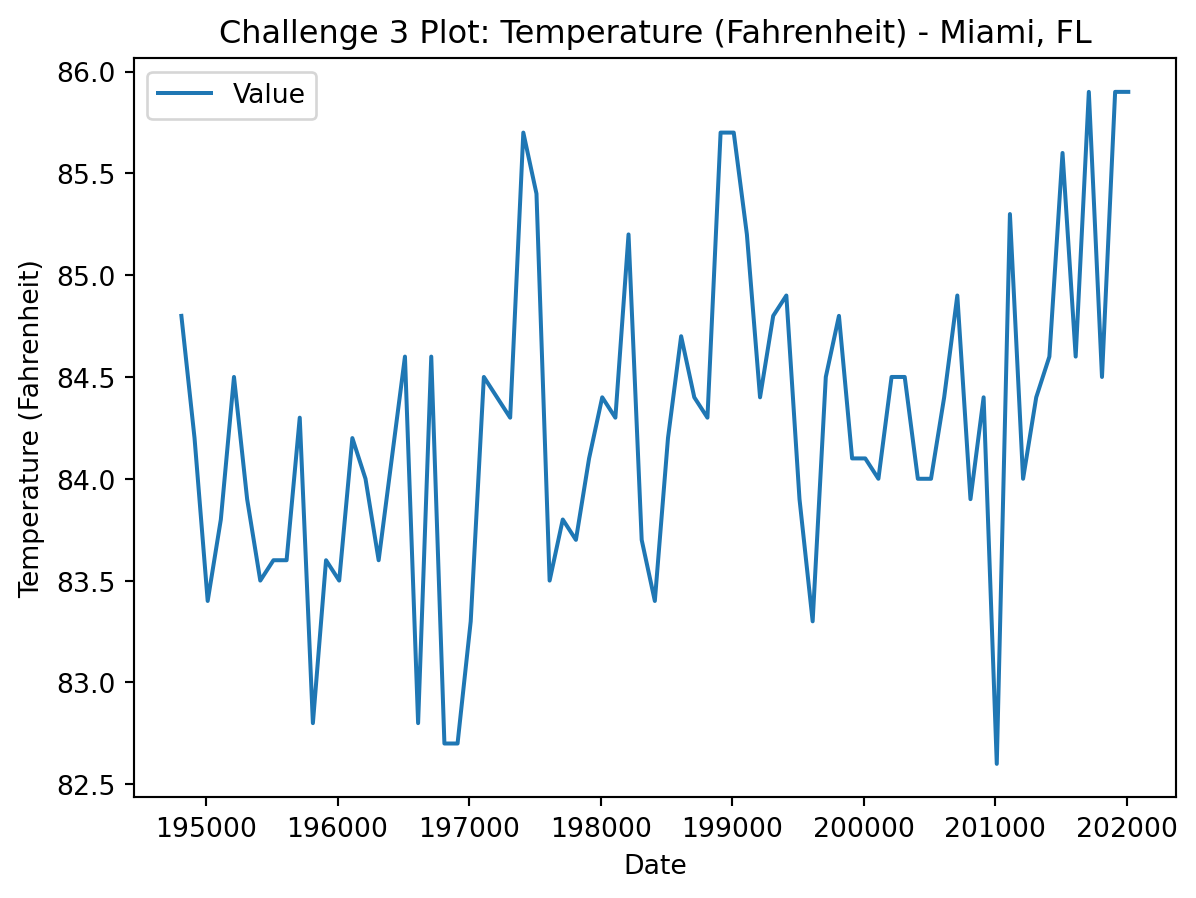
\includegraphics[keepaspectratio]{notebooks/05-vegetation/vegetation-download-shortcourse_files/figure-pdf/cell-10-output-1.png}}

We have a map of \textbf{?meta:params.short\_name}!

\bookmarksetup{startatroot}

\chapter{STEP 3: Save your OSM
download}\label{step-3-save-your-osm-download}

The Open Street Map API is pretty reliable, and it caches the results
automatically to avoid multiple downloads. However, you still might want
to save your download, for example to distribute as part of a data
release or reproducible workflow.

\begin{Shaded}
\begin{Highlighting}[]
\CommentTok{\# Create path for boundary}
\NormalTok{boundary\_path }\OperatorTok{=}\NormalTok{ project.project\_dir }\OperatorTok{/}\NormalTok{ boundary\_dirname}
\CommentTok{\# Can\textquotesingle{}t overwrite existing files, which seems to be an intractable GDAL issue}
\ControlFlowTok{if}\NormalTok{ boundary\_path.exists():}
\NormalTok{    shutil.rmtree(boundary\_path)}

\CommentTok{\# Write OSM result to shapefile}
\NormalTok{boundary\_gdf.to\_file(boundary\_path)}
\end{Highlighting}
\end{Shaded}

\bookmarksetup{startatroot}

\chapter{STEP 2: AppEEARS API}\label{step-2-appeears-api-1}

\section{Exploring the AppEEARS API for NASA Earthdata
access}\label{exploring-the-appeears-api-for-nasa-earthdata-access-1}

Before you get started with the data download today, you will need a
free \href{https://urs.earthdata.nasa.gov/home}{NASA Earthdata account}
if you don't have one already!

Over the next four cells, you will download MODIS NDVI data for the
study period. MODIS is a multispectral instrument that measures Red and
NIR data (and so can be used for NDVI). There are two MODIS sensors on
two different platforms: satellites Terra and Aqua.

\begin{tcolorbox}[enhanced jigsaw, colbacktitle=quarto-callout-color!10!white, opacityback=0, bottomtitle=1mm, toptitle=1mm, bottomrule=.15mm, left=2mm, colframe=quarto-callout-color-frame, leftrule=.75mm, opacitybacktitle=0.6, colback=white, rightrule=.15mm, toprule=.15mm, breakable, titlerule=0mm, title=\textcolor{quarto-callout-color}{\faInfo}\hspace{0.5em}{Read More}, coltitle=black, arc=.35mm]

\href{https://modis.gsfc.nasa.gov/}{Learn more about MODIS datasets and
the science they support}

\end{tcolorbox}

Since we're asking for a special download that only covers our study
area, we can't just find a link to the data - we have to negotiate with
the data server. We're doing this using the
\href{https://appeears.earthdatacloud.nasa.gov/api/}{APPEEARS} API
(Application Programming Interface). The API makes it possible for you
to request data using code. You can use code from the \texttt{earthpy}
library to handle the API request.

\begin{tcolorbox}[enhanced jigsaw, colbacktitle=quarto-callout-color!10!white, opacityback=0, bottomtitle=1mm, toptitle=1mm, bottomrule=.15mm, left=2mm, colframe=quarto-callout-color-frame, leftrule=.75mm, opacitybacktitle=0.6, colback=white, rightrule=.15mm, toprule=.15mm, breakable, titlerule=0mm, title=\textcolor{quarto-callout-color}{\faInfo}\hspace{0.5em}{Try It}, coltitle=black, arc=.35mm]

Often when we want to do something more complex in coding we find an
example and modify it. This download code is already almost a working
example. Your task will be:

\begin{enumerate}
\def\labelenumi{\arabic{enumi}.}
\tightlist
\item
  Replace the start and end dates in the task parameters. Download data
  from July, when greenery is at its peak in the Northern Hemisphere.
\item
  Replace the year range. You should get 3 years before and after the
  event so you can see the change!
\item
  Replace \texttt{gdf} with the name of \textbf{your} site geodataframe.
\item
  \textbf{Enter your NASA Earthdata username and password when
  prompted.} The prompts can be a little hard to see -- look at the top
  of your screen!
\end{enumerate}

\end{tcolorbox}

\begin{tcolorbox}[enhanced jigsaw, colbacktitle=quarto-callout-color!10!white, opacityback=0, bottomtitle=1mm, toptitle=1mm, bottomrule=.15mm, left=2mm, colframe=quarto-callout-color-frame, leftrule=.75mm, opacitybacktitle=0.6, colback=white, rightrule=.15mm, toprule=.15mm, breakable, titlerule=0mm, title=\textcolor{quarto-callout-color}{\faInfo}\hspace{0.5em}{Reflect and Respond}, coltitle=black, arc=.35mm]

What would the product and layer name be if you were trying to download
Landsat Surface Temperature Analysis Ready Data (ARD) instead of MODIS
NDVI?

\end{tcolorbox}

\begin{tcolorbox}[enhanced jigsaw, colbacktitle=quarto-callout-important-color!10!white, opacityback=0, bottomtitle=1mm, toptitle=1mm, bottomrule=.15mm, left=2mm, colframe=quarto-callout-important-color-frame, leftrule=.75mm, opacitybacktitle=0.6, colback=white, rightrule=.15mm, toprule=.15mm, breakable, titlerule=0mm, title=\textcolor{quarto-callout-important-color}{\faExclamation}\hspace{0.5em}{Important}, coltitle=black, arc=.35mm]

It can take some time for Appeears to process your request - anything
from a few minutes to a few hours depending on how busy they are. You
can check your progress by:

\begin{enumerate}
\def\labelenumi{\arabic{enumi}.}
\tightlist
\item
  Going to the \href{https://appeears.earthdatacloud.nasa.gov/}{Appeears
  webpage}
\item
  Clicking the \texttt{Explore} tab
\item
  Logging in with your Earthdata account
\end{enumerate}

\end{tcolorbox}

\begin{Shaded}
\begin{Highlighting}[]
\CommentTok{\# Initialize AppeearsDownloader for MODIS NDVI data}
\NormalTok{ndvi\_downloader }\OperatorTok{=}\NormalTok{ eaapp.AppeearsDownloader(}
\NormalTok{    download\_key}\OperatorTok{=}\NormalTok{download\_key,}
\NormalTok{    product}\OperatorTok{=}\StringTok{\textquotesingle{}MOD13Q1.061\textquotesingle{}}\NormalTok{,}
\NormalTok{    layer}\OperatorTok{=}\StringTok{\textquotesingle{}\_250m\_16\_days\_NDVI\textquotesingle{}}\NormalTok{,}
\NormalTok{    start\_date}\OperatorTok{=}\StringTok{\textquotesingle{}01{-}01\textquotesingle{}}\NormalTok{,}
\NormalTok{    end\_date}\OperatorTok{=}\StringTok{\textquotesingle{}01{-}31\textquotesingle{}}\NormalTok{,}
\NormalTok{    recurring}\OperatorTok{=}\VariableTok{True}\NormalTok{,}
\NormalTok{    year\_range}\OperatorTok{=}\NormalTok{[, ],}
\NormalTok{    polygon}\OperatorTok{=}\NormalTok{gdf}
\NormalTok{)}
\CommentTok{\# Download the prepared download {-}{-} this can take some time!}
\NormalTok{ndvi\_downloader.download\_files(cache}\OperatorTok{=}\VariableTok{True}\NormalTok{)}
\end{Highlighting}
\end{Shaded}

\section{Putting it together: Working with multi-file raster datasets in
Python}\label{putting-it-together-working-with-multi-file-raster-datasets-in-python-1}

Now you need to load all the downloaded files into Python. You may have
noticed that the `earthpy.appears module gives us all the downloaded
file names\ldots but only some of those are the NDVI files we want while
others are quality files that tell us about the confidence in the
dataset. For now, the files we want all have ``NDVI'' in the name.

Let's start by getting all the NDVI file names. You will also need to
extract the date from the filename. Check out
\href{https://www.earthdatascience.org/courses/intro-to-earth-data-science/write-efficient-python-code/loops/data-workflows-with-loops/}{the
lesson on getting information from filenames in the textbook}. We're
using a slightly different method here (the \texttt{.rglob()} or
\textbf{recursive} glob method, which searchs all the directories nested
inside the path), but the principle is the same.

\begin{tcolorbox}[enhanced jigsaw, colbacktitle=quarto-callout-caution-color!10!white, opacityback=0, bottomtitle=1mm, toptitle=1mm, bottomrule=.15mm, left=2mm, colframe=quarto-callout-caution-color-frame, leftrule=.75mm, opacitybacktitle=0.6, colback=white, rightrule=.15mm, toprule=.15mm, breakable, titlerule=0mm, title=\textcolor{quarto-callout-caution-color}{\faFire}\hspace{0.5em}{GOTCHA ALERT!}, coltitle=black, arc=.35mm]

\texttt{glob} doesn't necessarily find files in the order you would
expect. Make sure to \textbf{sort} your file names like it says in the
textbook.

\end{tcolorbox}

\begin{Shaded}
\begin{Highlighting}[]
\CommentTok{\# Get a sorted list of NDVI tif file paths}
\NormalTok{ndvi\_paths }\OperatorTok{=} \BuiltInTok{sorted}\NormalTok{(}\BuiltInTok{list}\NormalTok{(project.project\_dir.rglob(}\StringTok{\textquotesingle{}ndvi{-}pattern\textquotesingle{}}\NormalTok{)))}

\CommentTok{\# Display the first and last three files paths to check the pattern}
\NormalTok{ndvi\_paths[:}\DecValTok{3}\NormalTok{], ndvi\_paths[}\OperatorTok{{-}}\DecValTok{3}\NormalTok{:]}
\end{Highlighting}
\end{Shaded}

\subsection{Repeating tasks in
Python}\label{repeating-tasks-in-python-3}

Now you should have a few dozen files! For each file, you need to:

\begin{itemize}
\tightlist
\item
  Load the file in using the \texttt{rioxarray} library
\item
  Get the date from the file name
\item
  Add the date as a dimension coordinate
\item
  Give your data variable a name
\end{itemize}

You don't want to write out the code for each file! That's a recipe for
\textbf{copy pasta} and errors. Luckily, Python has tools for doing
similar tasks repeatedly. In this case, you'll use one called a
\texttt{for} loop.

There's some code below that uses a \texttt{for} loop in what is called
an \textbf{accumulation pattern} to process each file. That means that
you will save the results of your processing to a list each time you
process the files, and then merge all the arrays in the list.

\begin{tcolorbox}[enhanced jigsaw, colbacktitle=quarto-callout-color!10!white, opacityback=0, bottomtitle=1mm, toptitle=1mm, bottomrule=.15mm, left=2mm, colframe=quarto-callout-color-frame, leftrule=.75mm, opacitybacktitle=0.6, colback=white, rightrule=.15mm, toprule=.15mm, breakable, titlerule=0mm, title=\textcolor{quarto-callout-color}{\faInfo}\hspace{0.5em}{Try It}, coltitle=black, arc=.35mm]

\begin{itemize}
\tightlist
\item
  Look at the file names. How many characters from the end is the date?
  \texttt{doy\_start} and \texttt{doy\_end} are used to extract the day
  of the year (doy) from the file name. You will need to count
  characters from the end and change the values to get the right part of
  the file name. HINT: the index -1 in Python means the last value, -2
  second-to-last, and so on.
\item
  Replace any required variable names with your chosen variable names
\end{itemize}

\end{tcolorbox}

\begin{Shaded}
\begin{Highlighting}[]
\NormalTok{doy\_start }\OperatorTok{=} \OperatorTok{{-}}\DecValTok{1}
\NormalTok{doy\_end }\OperatorTok{=} \OperatorTok{{-}}\DecValTok{1}

\CommentTok{\# Loop through each NDVI image}
\NormalTok{ndvi\_das }\OperatorTok{=}\NormalTok{ []}
\ControlFlowTok{for}\NormalTok{ ndvi\_path }\KeywordTok{in}\NormalTok{ ndvi\_paths:}
    \CommentTok{\# Get date from file name}

    \CommentTok{\# Open dataset}

    \CommentTok{\# Add date dimension and clean up metadata}
\NormalTok{    da }\OperatorTok{=}\NormalTok{ da.assign\_coords(\{}\StringTok{\textquotesingle{}date\textquotesingle{}}\NormalTok{: date\})}
\NormalTok{    da }\OperatorTok{=}\NormalTok{ da.expand\_dims(\{}\StringTok{\textquotesingle{}date\textquotesingle{}}\NormalTok{: }\DecValTok{1}\NormalTok{\})}
\NormalTok{    da.name }\OperatorTok{=} \StringTok{\textquotesingle{}NDVI\textquotesingle{}}

    \CommentTok{\# Prepare for concatenation}
\end{Highlighting}
\end{Shaded}

\begin{tcolorbox}[enhanced jigsaw, colbacktitle=quarto-callout-color!10!white, opacityback=0, bottomtitle=1mm, toptitle=1mm, bottomrule=.15mm, left=2mm, colframe=quarto-callout-color-frame, leftrule=.75mm, opacitybacktitle=0.6, colback=white, rightrule=.15mm, toprule=.15mm, breakable, titlerule=0mm, title=\textcolor{quarto-callout-color}{\faInfo}\hspace{0.5em}{Try It}, coltitle=black, arc=.35mm]

Next, stack your arrays by date into a time series:

\begin{enumerate}
\def\labelenumi{\arabic{enumi}.}
\tightlist
\item
  Modify the code to match your prior workflow steps and to use
  descriptive variable names
\item
  Replace \texttt{coordinate\_name} with the actual name of the
  coordinate you want to build up.
\end{enumerate}

\end{tcolorbox}

\begin{Shaded}
\begin{Highlighting}[]
\CommentTok{\# Combine NDVI images from all dates}
\NormalTok{da }\OperatorTok{=}\NormalTok{ xr.combine\_by\_coords(list\_of\_data\_arrays, coords}\OperatorTok{=}\NormalTok{[}\StringTok{\textquotesingle{}coordinate\_name\textquotesingle{}}\NormalTok{])}
\NormalTok{da}
\end{Highlighting}
\end{Shaded}

\section{Your turn! Repeat this workflow in a different time and
place.}\label{your-turn-repeat-this-workflow-in-a-different-time-and-place.-1}

It's not only irrigation that affects NDVI! You could look at:

\begin{itemize}
\tightlist
\item
  Recovery after a national disaster, like a wildfire or hurricane
\item
  Drought
\item
  Deforestation
\item
  Irrigation
\item
  Beaver reintroduction
\end{itemize}

\bookmarksetup{startatroot}

\chapter{Climate Coding Challenge}\label{climate-coding-challenge-1}

Climate change is impacting the way people live around the world

\hfill\break

\bookmarksetup{startatroot}

\chapter{Part 1: Overview}\label{part-1-overview-1}

Higher highs, lower lows, storms, and smoke -- we're all feeling the
effects of climate change. In this workflow, you will take a look at
trends in temperature over time in \textbf{?meta:params.location}.

\begin{tcolorbox}[enhanced jigsaw, colbacktitle=quarto-callout-color!10!white, opacityback=0, bottomtitle=1mm, toptitle=1mm, bottomrule=.15mm, left=2mm, colframe=quarto-callout-color-frame, leftrule=.75mm, opacitybacktitle=0.6, colback=white, rightrule=.15mm, toprule=.15mm, breakable, titlerule=0mm, title=\textcolor{quarto-callout-color}{\faInfo}\hspace{0.5em}{Conversation Starter}, coltitle=black, arc=.35mm]

In a few sentences, how is climate change affecting your home?

\end{tcolorbox}

\section{What the fork?! Who wrote
this?}\label{what-the-fork-who-wrote-this-1}

For this challenge, you'll be running a scientific workflow in Python.
But something's wrong -- The code won't run! Your task is to follow the
instructions below to \textbf{clean and debug} the Python code below so
that it runs.

\begin{tcolorbox}[enhanced jigsaw, colbacktitle=quarto-callout-tip-color!10!white, opacityback=0, bottomtitle=1mm, toptitle=1mm, bottomrule=.15mm, left=2mm, colframe=quarto-callout-tip-color-frame, leftrule=.75mm, opacitybacktitle=0.6, colback=white, rightrule=.15mm, toprule=.15mm, breakable, titlerule=0mm, title=\textcolor{quarto-callout-tip-color}{\faLightbulb}\hspace{0.5em}{Tip}, coltitle=black, arc=.35mm]

Don't worry if you can't solve every bug right away. We'll get there! If
you are working on one bug for more than about 10 minutes, it's time to
ask for help.

\end{tcolorbox}

At the end, you'll \textbf{repeat the workflow} for a location and
measurement of your choosing.

Alright! Let's clean up this code.

Before we get started, let's define some parameters. You can use these
if you want to change how the workflow runs from the top:

\begin{Shaded}
\begin{Highlighting}[]
\BuiltInTok{id} \OperatorTok{=} \StringTok{\textquotesingle{}eda\textquotesingle{}}
\NormalTok{ncei\_filename }\OperatorTok{=} \StringTok{\textquotesingle{}ncei{-}climate{-}boulder.csv\textquotesingle{}}
\NormalTok{project\_name }\OperatorTok{=} \StringTok{\textquotesingle{}Boulder Climate\textquotesingle{}}
\NormalTok{location }\OperatorTok{=} \StringTok{\textquotesingle{}Boulder, CO\textquotesingle{}}
\NormalTok{station\_id }\OperatorTok{=} \StringTok{\textquotesingle{}USC00050848\textquotesingle{}}
\NormalTok{start\_date }\OperatorTok{=} \StringTok{\textquotesingle{}1893{-}10{-}01\textquotesingle{}}
\NormalTok{end\_date }\OperatorTok{=} \StringTok{\textquotesingle{}2023{-}09{-}30\textquotesingle{}}
\NormalTok{data\_type }\OperatorTok{=} \StringTok{\textquotesingle{}TOBS\textquotesingle{}}
\end{Highlighting}
\end{Shaded}

\bookmarksetup{startatroot}

\chapter{STEP 2: Wrangle your data}\label{step-2-wrangle-your-data-1}

\section{\texorpdfstring{Python \textbf{packages} let you use code
written by experts around the
world}{Python packages let you use code written by experts around the world}}\label{python-packages-let-you-use-code-written-by-experts-around-the-world-1}

Because Python is open source, lots of different people and
organizations can contribute (including you!). Many contributions are in
the form of \textbf{packages} which do not come with a standard Python
download.

\begin{tcolorbox}[enhanced jigsaw, colbacktitle=quarto-callout-color!10!white, opacityback=0, bottomtitle=1mm, toptitle=1mm, bottomrule=.15mm, left=2mm, colframe=quarto-callout-color-frame, leftrule=.75mm, opacitybacktitle=0.6, colback=white, rightrule=.15mm, toprule=.15mm, breakable, titlerule=0mm, title=\textcolor{quarto-callout-color}{\faInfo}\hspace{0.5em}{Read More: Packages need to be installed and imported.}, coltitle=black, arc=.35mm]

Learn more about using Python packages. How do you find and use
packages? What is the difference between installing and importing
packages? When do you need to do each one?
\href{https://www.earthdatascience.org/courses/intro-to-earth-data-science/python-code-fundamentals/use-python-packages/}{This
article on Python packages} will walk you through the basics.

\end{tcolorbox}

In the cell below, someone was trying to import the \textbf{pandas
package}, which helps us to work with
\href{https://www.earthdatascience.org/courses/intro-to-earth-data-science/file-formats/use-text-files/}{\textbf{tabular
data} such as comma-separated value or csv files}. But something's
wrong!

\begin{tcolorbox}[enhanced jigsaw, colbacktitle=quarto-callout-color!10!white, opacityback=0, bottomtitle=1mm, toptitle=1mm, bottomrule=.15mm, left=2mm, colframe=quarto-callout-color-frame, leftrule=.75mm, opacitybacktitle=0.6, colback=white, rightrule=.15mm, toprule=.15mm, breakable, titlerule=0mm, title=\textcolor{quarto-callout-color}{\faInfo}\hspace{0.5em}{Try It: Import packages}, coltitle=black, arc=.35mm]

\begin{enumerate}
\def\labelenumi{\arabic{enumi}.}
\tightlist
\item
  Correct the typo below to properly import the pandas package under its
  \textbf{alias} pd.
\item
  Run the cell to import the libraries you'll need for this workflow.
\end{enumerate}

\end{tcolorbox}

\begin{Shaded}
\begin{Highlighting}[]
\CommentTok{\# Import libraries}
\ImportTok{import}\NormalTok{ earthpy}
\ImportTok{import}\NormalTok{ holoviews }\ImportTok{as}\NormalTok{ hv}
\ImportTok{import}\NormalTok{ hvplot.pandas}
\ImportTok{import}\NormalTok{ pandsa }\ImportTok{as}\NormalTok{ pd}
\end{Highlighting}
\end{Shaded}

\section{Download the practice data}\label{download-the-practice-data-1}

Next, lets download some climate data from
\textbf{?meta:params.location} to practice with.

\begin{enumerate}
\def\labelenumi{\arabic{enumi}.}
\tightlist
\item
  It is surrounded by quotes -- that means Python will interpret it as a
  \texttt{character\ string}, or text, rather than which makes sense for
  a URL.
\item
  The URL is too long to display as one line on most screens. We've put
  parentheses around it so that we can easily split it into multiple
  lines by writing two strings -- one on each line.
\item
  We replaced the figshare identifier for this dataset with
  \texttt{\textquotesingle{}FIGSHARE\_ID\_HERE\textquotesingle{}}.
  You'll have to replace that with the real identifier,
  \textbf{?meta:params.figshare\_id}
\end{enumerate}

However, we still have a problem - we can't get the URL back later on
because it isn't saved in a \textbf{variable}. In other words, we need
to give the url a \textbf{name} so that we can request in from Python
later (sadly, Python has no `hey what was that thingy I typed
yesterday?' function).

\begin{tcolorbox}[enhanced jigsaw, colbacktitle=quarto-callout-color!10!white, opacityback=0, bottomtitle=1mm, toptitle=1mm, bottomrule=.15mm, left=2mm, colframe=quarto-callout-color-frame, leftrule=.75mm, opacitybacktitle=0.6, colback=white, rightrule=.15mm, toprule=.15mm, breakable, titlerule=0mm, title=\textcolor{quarto-callout-color}{\faInfo}\hspace{0.5em}{Read More: Names/variables in Python}, coltitle=black, arc=.35mm]

One of the most common challenges for new programmers is making sure
that your results are stored so you can use them again. In Python, this
is called \textbf{naming}, or saving a \textbf{variable}. Learn more in
this
\href{https://www.earthdatascience.org/courses/intro-to-earth-data-science/python-code-fundamentals/get-started-using-python/variables/}{hands-on
activity on using variables} from our learning portal.

\end{tcolorbox}

\begin{tcolorbox}[enhanced jigsaw, colbacktitle=quarto-callout-color!10!white, opacityback=0, bottomtitle=1mm, toptitle=1mm, bottomrule=.15mm, left=2mm, colframe=quarto-callout-color-frame, leftrule=.75mm, opacitybacktitle=0.6, colback=white, rightrule=.15mm, toprule=.15mm, breakable, titlerule=0mm, title=\textcolor{quarto-callout-color}{\faInfo}\hspace{0.5em}{Try It: Save the URL for later}, coltitle=black, arc=.35mm]

\begin{enumerate}
\def\labelenumi{\arabic{enumi}.}
\tightlist
\item
  Replace \texttt{Project\ Name\ Here} with the actual project name,
  \textbf{?meta:params.project\_name}.
\item
  Replace \texttt{data-folder-name-here} with a \emph{descriptive} name
  for your data folder.
\item
  Run the cell. Can you find the data on your computer?
\end{enumerate}

\end{tcolorbox}

\begin{Shaded}
\begin{Highlighting}[]
\CommentTok{\# Set up project folders}
\NormalTok{project }\OperatorTok{=}\NormalTok{ earthpy.Project(}
    \StringTok{\textquotesingle{}Project Name Here\textquotesingle{}}\NormalTok{,}
\NormalTok{    dirname}\OperatorTok{=}\StringTok{\textquotesingle{}data{-}folder{-}name{-}here\textquotesingle{}}\NormalTok{)}

\CommentTok{\# Download data}
\NormalTok{project.get\_data()}

\CommentTok{\# Check where the data ended up}
\NormalTok{project.project\_dir}
\end{Highlighting}
\end{Shaded}

If you are on GitHub Codespaces, you should be able to see your data in
your \texttt{Explorer} tab.

\begin{figure}[H]

{\centering \pandocbounded{\includegraphics[keepaspectratio]{notebooks/01-climate/.pdf}}

}

\caption{You can find the Explorer tab on the left hand side of the
screen. Your data should be in the \texttt{data} folder mounted there.}

\end{figure}%

You can also take a look at your data using \texttt{bash}, either in
your terminal or here in your Jupyter notebook:

\begin{Shaded}
\begin{Highlighting}[]
\OperatorTok{\%\%}\NormalTok{bash}
\NormalTok{ls $(project.project\_dir)}
\end{Highlighting}
\end{Shaded}

\begin{verbatim}
bash: line 1: project.project_dir: command not found
\end{verbatim}

\begin{verbatim}
_climate-01-machine-readable.qmd
_climate-11-python-as-a-calculator.qmd
_climate-30-overview.qmd
_climate-32-wrangle.qmd
_climate-33-units.qmd
_climate-34-plot.qmd
_climate-35-trend-line.qmd
_climate-98-download.qmd
_climate-99-portfolio.qmd
annual_climate.html
climate-download-css.qmd
climate-download-eda_files
climate-download-eda.html
climate-download-eda.qmd
climate-download-shortcourse_files
climate-download-shortcourse.qmd
climate-eda_files
climate-eda.html
climate-eda.qmd
climate-eda.quarto_ipynb
climate-shortcourse_files
climate-shortcourse.qmd
climate-stars.qmd
segments-eda
segments-foundations
segments-shortcourse
\end{verbatim}

The \texttt{pandas} library you imported can download data from the
internet directly into a type of Python \textbf{object} called a
\texttt{DataFrame}. In the code cell below, you can see an attempt to do
just this. But there are some problems\ldots{}

\begin{tcolorbox}[enhanced jigsaw, colbacktitle=quarto-callout-color!10!white, opacityback=0, bottomtitle=1mm, toptitle=1mm, bottomrule=.15mm, left=2mm, colframe=quarto-callout-color-frame, leftrule=.75mm, opacitybacktitle=0.6, colback=white, rightrule=.15mm, toprule=.15mm, breakable, titlerule=0mm, title=\textcolor{quarto-callout-color}{\faInfo}\hspace{0.5em}{Try It: Fix some code!}, coltitle=black, arc=.35mm]

\begin{enumerate}
\def\labelenumi{\arabic{enumi}.}
\item
  Leave a space between the \texttt{\#} and text in the comment,
  capitalize it, and try to make it more informative
\item
  Make any changes needed to get this code to run. HINT: The
  \texttt{my\_url} variable doesn't exist - you need to replace it with
  the variable name \textbf{you} chose.
\item
  Modify the \texttt{.read\_csv()} function call to include the
  following parameters:

  \begin{itemize}
  \tightlist
  \item
    \texttt{index\_col=\textquotesingle{}DATE\textquotesingle{}} -- this
    sets the \texttt{DATE} column as the index. Needed for subsetting
    and resampling later on
  \item
    \texttt{parse\_dates=True} -- this lets \texttt{python} know that
    you are working with time-series data, and values in the indexed
    column are \textbf{date time objects}
  \item
    \texttt{na\_values={[}\textquotesingle{}NaN\textquotesingle{}{]}} --
    this lets \texttt{python} know how to handle missing values
  \end{itemize}
\item
  Clean up the code by using \textbf{expressive variable names},
  \textbf{expressive column names}, \textbf{PEP-8 compliant code}, and
  \textbf{descriptive comments}
\end{enumerate}

\end{tcolorbox}

\begin{Shaded}
\begin{Highlighting}[]
\CommentTok{\#download}
\NormalTok{climate\_df }\OperatorTok{=}\NormalTok{ pd.read\_csv(}
\NormalTok{    project.project\_dir }\OperatorTok{/} \StringTok{\textquotesingle{}filename.csv\textquotesingle{}}\NormalTok{,}
    \CommentTok{\#index\_col=\textquotesingle{}something\textquotesingle{})}
\NormalTok{climate\_df}
\end{Highlighting}
\end{Shaded}

\begin{tcolorbox}[enhanced jigsaw, colbacktitle=quarto-callout-tip-color!10!white, opacityback=0, bottomtitle=1mm, toptitle=1mm, bottomrule=.15mm, left=2mm, colframe=quarto-callout-tip-color-frame, leftrule=.75mm, opacitybacktitle=0.6, colback=white, rightrule=.15mm, toprule=.15mm, breakable, titlerule=0mm, title=\textcolor{quarto-callout-tip-color}{\faLightbulb}\hspace{0.5em}{Tip}, coltitle=black, arc=.35mm]

Check out the \texttt{type()} function below - you can use it to check
that your data is now in \texttt{DataFrame} type object.

\end{tcolorbox}

\begin{Shaded}
\begin{Highlighting}[]
\CommentTok{\# Check that the data was imported into a pandas DataFrame}
\BuiltInTok{type}\NormalTok{(climate\_df)}
\end{Highlighting}
\end{Shaded}

\section{\texorpdfstring{Clean up your
\texttt{DataFrame}}{Clean up your DataFrame}}\label{clean-up-your-dataframe-1}

\begin{tcolorbox}[enhanced jigsaw, colbacktitle=quarto-callout-color!10!white, opacityback=0, bottomtitle=1mm, toptitle=1mm, bottomrule=.15mm, left=2mm, colframe=quarto-callout-color-frame, leftrule=.75mm, opacitybacktitle=0.6, colback=white, rightrule=.15mm, toprule=.15mm, breakable, titlerule=0mm, title=\textcolor{quarto-callout-color}{\faInfo}\hspace{0.5em}{Try It: Get rid of unwanted columns}, coltitle=black, arc=.35mm]

You can use \textbf{double brackets} (\texttt{{[}{[}} and
\texttt{{]}{]}}) to select only the columns that you want from your
\texttt{DataFrame}:

\begin{enumerate}
\def\labelenumi{\arabic{enumi}.}
\tightlist
\item
  Change \texttt{some\_column\_name} to the Temperature column name.
\item
  Give the \texttt{DataFrame} a more descriptive name.
\item
  Add a properly formatted comment to describe what this code is doing.
\end{enumerate}

\end{tcolorbox}

\begin{tcolorbox}[enhanced jigsaw, colbacktitle=quarto-callout-warning-color!10!white, opacityback=0, bottomtitle=1mm, toptitle=1mm, bottomrule=.15mm, left=2mm, colframe=quarto-callout-warning-color-frame, leftrule=.75mm, opacitybacktitle=0.6, colback=white, rightrule=.15mm, toprule=.15mm, breakable, titlerule=0mm, title=\textcolor{quarto-callout-warning-color}{\faExclamationTriangle}\hspace{0.5em}{Warning}, coltitle=black, arc=.35mm]

Column names are text values, not variable names, so you need to put
them in quotes!

\end{tcolorbox}

\begin{Shaded}
\begin{Highlighting}[]
\NormalTok{climate\_df }\OperatorTok{=}\NormalTok{ climate\_df[[}\StringTok{\textquotesingle{}some\_column\_name\textquotesingle{}}\NormalTok{]]}
\NormalTok{climate\_df}
\end{Highlighting}
\end{Shaded}

\bookmarksetup{startatroot}

\chapter{STEP 3: Convert units}\label{step-3-convert-units-1}

It's important to keep track of the units of all your data. You don't
want to be like the
\href{https://www.latimes.com/archives/la-xpm-1999-oct-01-mn-17288-story.html}{NASA
team who crashed a probe into Mars because different teams used
different units})!

\section{Use labels to keep track of units for you and your
collaborators}\label{use-labels-to-keep-track-of-units-for-you-and-your-collaborators-1}

One way to keep track of your data's units is to include the unit in
data \textbf{labels}. In the case of a \texttt{DataFrame}, that usually
means the column names.

\begin{tcolorbox}[enhanced jigsaw, colbacktitle=quarto-callout-color!10!white, opacityback=0, bottomtitle=1mm, toptitle=1mm, bottomrule=.15mm, left=2mm, colframe=quarto-callout-color-frame, leftrule=.75mm, opacitybacktitle=0.6, colback=white, rightrule=.15mm, toprule=.15mm, breakable, titlerule=0mm, title=\textcolor{quarto-callout-color}{\faInfo}\hspace{0.5em}{Try It: Add units to your column name}, coltitle=black, arc=.35mm]

A big part of writing \textbf{expressive} code is descriptive labels.
Let's rename the columns of your dataframe to include units. Complete
the following steps:

\begin{enumerate}
\def\labelenumi{\arabic{enumi}.}
\tightlist
\item
  Replace \texttt{dataframe} with the name of \textbf{your}
  \texttt{DataFrame}, and \texttt{dataframe\_units} with an expressive
  new name.
\item
  Check out the
  \href{https://www.ncei.noaa.gov/data/global-historical-climatology-network-daily/doc/GHCND_documentation.pdf}{documentation
  for GCHNd data}. We downloaded data with ``standard'' units; find out
  what that means for both temperature and precipitation.
\item
  Replace \texttt{\textquotesingle{}TOBS\textquotesingle{}} with the
  temperature column name in your data, and
  \texttt{\textquotesingle{}TOBS\_UNIT\textquotesingle{}} with a column
  name that includes the correct unit.
\end{enumerate}

\end{tcolorbox}

\begin{Shaded}
\begin{Highlighting}[]
\NormalTok{dataframe\_units }\OperatorTok{=}\NormalTok{ dataframe.rename(columns}\OperatorTok{=}\NormalTok{\{}
    \StringTok{\textquotesingle{}TOBS\textquotesingle{}}\NormalTok{: }\StringTok{\textquotesingle{}TOBS\_UNIT\textquotesingle{}}\NormalTok{,}
\NormalTok{\})}

\NormalTok{dataframe\_units}
\end{Highlighting}
\end{Shaded}

\section{For scientific applications, it is often useful to have values
in metric
units}\label{for-scientific-applications-it-is-often-useful-to-have-values-in-metric-units-1}

\begin{tcolorbox}[enhanced jigsaw, colbacktitle=quarto-callout-color!10!white, opacityback=0, bottomtitle=1mm, toptitle=1mm, bottomrule=.15mm, left=2mm, colframe=quarto-callout-color-frame, leftrule=.75mm, opacitybacktitle=0.6, colback=white, rightrule=.15mm, toprule=.15mm, breakable, titlerule=0mm, title=\textcolor{quarto-callout-color}{\faInfo}\hspace{0.5em}{Try It: Convert units}, coltitle=black, arc=.35mm]

The code below attempts to convert the data to Celcius, using Python
mathematical \textbf{operators}, like \texttt{+}, \texttt{-},
\texttt{*}, and \texttt{/}. Mathematical operators in Python work just
like a calculator, and that includes using parentheses to designat the
\textbf{order of operations}. The equation for converting Fahrenheit
temperature to Celcius is:

\[ T_C = (T_F - 32) * \frac{5}{9} \]

This code is not well documented and doesn't follow
\href{https://peps.python.org/pep-0008/\#other-recommendations}{PEP-8
guidelines}, which has caused the author to miss an \textbf{important
error}!

Complete the following steps:

\begin{enumerate}
\def\labelenumi{\arabic{enumi}.}
\tightlist
\item
  Replace \texttt{dataframe} with the name of \textbf{your}
  \texttt{DataFrame}.
\item
  Replace \texttt{\textquotesingle{}old\_temperature\textquotesingle{}}
  with the column name \textbf{you} used; Replace
  \texttt{\textquotesingle{}new\_temperature\textquotesingle{}} with an
  \textbf{expressive} column name.
\item
  \textbf{THERE IS AN ERROR IN THE CONVERSION MATH - Fix it!}
\end{enumerate}

\end{tcolorbox}

\begin{Shaded}
\begin{Highlighting}[]
\NormalTok{dataframe\_units[}\StringTok{\textquotesingle{}new\_temperature\textquotesingle{}}\NormalTok{]}\OperatorTok{=}\NormalTok{ dataframe\_units[}\StringTok{\textquotesingle{}old\_temperature\textquotesingle{}}\NormalTok{]}\OperatorTok{{-}}\DecValTok{32}\OperatorTok{*}\DecValTok{5}\OperatorTok{/}\DecValTok{9}
\NormalTok{dataframe\_units}
\end{Highlighting}
\end{Shaded}

\begin{tcolorbox}[enhanced jigsaw, colbacktitle=quarto-callout-color!10!white, opacityback=0, bottomtitle=1mm, toptitle=1mm, bottomrule=.15mm, left=2mm, colframe=quarto-callout-color-frame, leftrule=.75mm, opacitybacktitle=0.6, colback=white, rightrule=.15mm, toprule=.15mm, breakable, titlerule=0mm, title=\textcolor{quarto-callout-color}{\faInfo}\hspace{0.5em}{Looking for an Extra Challenge?}, coltitle=black, arc=.35mm]

Using the code below as a framework, write and apply a \textbf{function}
that converts to Celcius. You should also rewrite this function name to
be more expressive.

\end{tcolorbox}

\begin{Shaded}
\begin{Highlighting}[]
\CommentTok{\# Convert units with a function}
\KeywordTok{def}\NormalTok{ convert(temperature):}
    \CommentTok{"""Convert temperature to Celcius"""}
    \ControlFlowTok{return}\NormalTok{ temperature }\CommentTok{\# Put your equation in here}

\NormalTok{dataframe[}\StringTok{\textquotesingle{}TEMP\_C\textquotesingle{}}\NormalTok{] }\OperatorTok{=}\NormalTok{ (}
\NormalTok{    dataframe[}\StringTok{\textquotesingle{}TEMP\_F\textquotesingle{}}\NormalTok{].}\BuiltInTok{apply}\NormalTok{(convert))}
\end{Highlighting}
\end{Shaded}

\begin{Shaded}
\begin{Highlighting}[]
\KeywordTok{def}\NormalTok{ convert\_f\_to\_c(temperature\_f):}
    \CommentTok{"""Convert temperature to Celcius"""}
    \ControlFlowTok{return}\NormalTok{ (temperature\_f }\OperatorTok{{-}} \DecValTok{32}\NormalTok{) }\OperatorTok{*} \DecValTok{5}\OperatorTok{/}\DecValTok{9}

\NormalTok{climate\_u\_df[}\StringTok{\textquotesingle{}temp\_c\textquotesingle{}}\NormalTok{] }\OperatorTok{=}\NormalTok{ (}
\NormalTok{    climate\_u\_df[}\StringTok{\textquotesingle{}temp\_f\textquotesingle{}}\NormalTok{].}\BuiltInTok{apply}\NormalTok{(convert\_f\_to\_c))}
\end{Highlighting}
\end{Shaded}

\bookmarksetup{startatroot}

\chapter{STEP 4: Plot your results}\label{step-4-plot-your-results-1}

\section{Plot the temperature column vs time to explore the
data}\label{plot-the-temperature-column-vs-time-to-explore-the-data-1}

Plotting in Python is easy, but not quite this easy:

\begin{Shaded}
\begin{Highlighting}[]
\NormalTok{climate\_u\_df.plot()}
\end{Highlighting}
\end{Shaded}

\pandocbounded{\includegraphics[keepaspectratio]{notebooks/01-climate/climate-eda_files/figure-pdf/cell-19-output-1.png}}

Looks like we have \emph{both} temperature units on the same plot, and
it's hard to see what it is because it's missing labels!

\begin{tcolorbox}[enhanced jigsaw, colbacktitle=quarto-callout-tip-color!10!white, opacityback=0, bottomtitle=1mm, toptitle=1mm, bottomrule=.15mm, left=2mm, colframe=quarto-callout-tip-color-frame, leftrule=.75mm, opacitybacktitle=0.6, colback=white, rightrule=.15mm, toprule=.15mm, breakable, titlerule=0mm, title=\textcolor{quarto-callout-tip-color}{\faLightbulb}\hspace{0.5em}{\textbf{Label your plot}}, coltitle=black, arc=.35mm]

\begin{figure}[H]

{\centering \pandocbounded{\includegraphics[keepaspectratio]{index_files/mediabag/convincing.png}}

}

\caption{Source: https://xkcd.com/833}

\end{figure}%

Make sure each plot has:

\begin{itemize}
\tightlist
\item
  A title that explains where and when the data are from
\item
  x- and y- axis labels with \textbf{units} where appropriate
\item
  A legend where appropriate
\end{itemize}

\end{tcolorbox}

When plotting in Python, you'll always need to add some instructions on
labels and how you want your plot to look.

\begin{tcolorbox}[enhanced jigsaw, colbacktitle=quarto-callout-color!10!white, opacityback=0, bottomtitle=1mm, toptitle=1mm, bottomrule=.15mm, left=2mm, colframe=quarto-callout-color-frame, leftrule=.75mm, opacitybacktitle=0.6, colback=white, rightrule=.15mm, toprule=.15mm, breakable, titlerule=0mm, title=\textcolor{quarto-callout-color}{\faInfo}\hspace{0.5em}{Try It: Plot your data}, coltitle=black, arc=.35mm]

\begin{enumerate}
\def\labelenumi{\arabic{enumi}.}
\tightlist
\item
  Change \texttt{dataframe} to \textbf{your} \texttt{DataFrame} name.
\item
  Change \texttt{y=} to the name of your \textbf{temperature} column
  name.
\item
  Use the \texttt{title}, \texttt{ylabel}, and \texttt{xlabel}
  parameters to add key text to your plot.
\item
  Adjust the size of your figure using \texttt{figsize=(x,y)} where
  \texttt{x} is figure width and \texttt{y} is figure height
\end{enumerate}

\end{tcolorbox}

\begin{tcolorbox}[enhanced jigsaw, colbacktitle=quarto-callout-tip-color!10!white, opacityback=0, bottomtitle=1mm, toptitle=1mm, bottomrule=.15mm, left=2mm, colframe=quarto-callout-tip-color-frame, leftrule=.75mm, opacitybacktitle=0.6, colback=white, rightrule=.15mm, toprule=.15mm, breakable, titlerule=0mm, title=\textcolor{quarto-callout-tip-color}{\faLightbulb}\hspace{0.5em}{Tip}, coltitle=black, arc=.35mm]

Labels have to be a \emph{type} in Python called a \textbf{string}. You
can make a string by putting quotes around your label, just like the
column names in the sample code (eg
\texttt{y=\textquotesingle{}temperature\textquotesingle{}}).

\end{tcolorbox}

\begin{Shaded}
\begin{Highlighting}[]
\CommentTok{\# Plot the data using .plot}
\NormalTok{climate\_u\_df.plot(}
\NormalTok{    y}\OperatorTok{=}\StringTok{\textquotesingle{}the\_temperature\_column\textquotesingle{}}\NormalTok{,}
\NormalTok{    title}\OperatorTok{=}\StringTok{\textquotesingle{}Title Goes Here\textquotesingle{}}\NormalTok{,}
\NormalTok{    xlabel}\OperatorTok{=}\StringTok{\textquotesingle{}Horizontal Axis Label Goes Here\textquotesingle{}}\NormalTok{,}
\NormalTok{    ylabel}\OperatorTok{=}\StringTok{\textquotesingle{}Vertical Axis Label Goes Here\textquotesingle{}}\NormalTok{)}
\end{Highlighting}
\end{Shaded}

\begin{tcolorbox}[enhanced jigsaw, colbacktitle=quarto-callout-color!10!white, opacityback=0, bottomtitle=1mm, toptitle=1mm, bottomrule=.15mm, left=2mm, colframe=quarto-callout-color-frame, leftrule=.75mm, opacitybacktitle=0.6, colback=white, rightrule=.15mm, toprule=.15mm, breakable, titlerule=0mm, title=\textcolor{quarto-callout-color}{\faInfo}\hspace{0.5em}{Looking for an Extra Challenge?}, coltitle=black, arc=.35mm]

There are many other things you can do to customize your plot. Take a
look at the
\href{https://pandas.pydata.org/docs/user_guide/visualization.html}{pandas
plotting galleries} and the
\href{https://pandas.pydata.org/docs/reference/api/pandas.DataFrame.plot.html}{documentation
of plot} to see if there's other changes you want to make to your plot.
Some possibilities include:

\begin{itemize}
\tightlist
\item
  Remove the legend since there's only one data series
\item
  Increase the figure size
\item
  Increase the font size
\item
  Change the colors
\item
  Use a bar graph instead (usually we use lines for time series, but
  since this is annual it could go either way)
\item
  Add a trend line
\end{itemize}

Not sure how to do any of these? Try searching the internet, or asking
an AI!

\end{tcolorbox}

\section{Clean up time series plots by
resampling}\label{clean-up-time-series-plots-by-resampling-1}

You may notice that your plot looks a little ``fuzzy''. This happens
when Python is trying to plot a value for every date, but the resolution
of the image is too low to actually do that. You can address this issue
by \textbf{resampling} the data, or summarizing it over a time period of
your choice. In this case, we will resample annually, giving us one data
point per year.

\begin{tcolorbox}[enhanced jigsaw, colbacktitle=quarto-callout-color!10!white, opacityback=0, bottomtitle=1mm, toptitle=1mm, bottomrule=.15mm, left=2mm, colframe=quarto-callout-color-frame, leftrule=.75mm, opacitybacktitle=0.6, colback=white, rightrule=.15mm, toprule=.15mm, breakable, titlerule=0mm, title=\textcolor{quarto-callout-color}{\faInfo}\hspace{0.5em}{Try It: Resample}, coltitle=black, arc=.35mm]

\begin{enumerate}
\def\labelenumi{\arabic{enumi}.}
\tightlist
\item
  Set the frequency of your final data by replacing
  \texttt{DT\_OFFSET}with a \textbf{Datetime Offset Code}. Check out the
  table in the
  \href{https://pandas.pydata.org/pandas-docs/stable/user_guide/timeseries.html\#dateoffset-objects}{pandas
  datetime documentation} to find the one you want (we recommend the
  start of the year).
\item
  Choose how to summarize each year of data by replacing
  \texttt{agg\_method\_here} with a method that will calculate the
  \textbf{average annual value}. Check out the
  \href{https://pandas.pydata.org/pandas-docs/stable/user_guide/timeseries.html\#basics}{pandas
  resampling documentation} for a list of common built-in options.
\end{enumerate}

\end{tcolorbox}

\begin{Shaded}
\begin{Highlighting}[]
\NormalTok{ann\_climate\_df }\OperatorTok{=}\NormalTok{ climate\_u\_df.resample(}\StringTok{\textquotesingle{}DT\_OFFSET\textquotesingle{}}\NormalTok{).agg\_method\_here()}
\NormalTok{ann\_climate\_df}
\end{Highlighting}
\end{Shaded}

\begin{tcolorbox}[enhanced jigsaw, colbacktitle=quarto-callout-color!10!white, opacityback=0, bottomtitle=1mm, toptitle=1mm, bottomrule=.15mm, left=2mm, colframe=quarto-callout-color-frame, leftrule=.75mm, opacitybacktitle=0.6, colback=white, rightrule=.15mm, toprule=.15mm, breakable, titlerule=0mm, title=\textcolor{quarto-callout-color}{\faInfo}\hspace{0.5em}{Try It: Plot Annual Data}, coltitle=black, arc=.35mm]

\begin{enumerate}
\def\labelenumi{\arabic{enumi}.}
\tightlist
\item
  Try plotting your new DataFrame in the cell below. Can you see what is
  going on more clearly now? Don't forget to adjust your labels!
\end{enumerate}

\end{tcolorbox}

\begin{Shaded}
\begin{Highlighting}[]
\CommentTok{\# Plot the annual data}
\end{Highlighting}
\end{Shaded}

\begin{tcolorbox}[enhanced jigsaw, colbacktitle=quarto-callout-color!10!white, opacityback=0, bottomtitle=1mm, toptitle=1mm, bottomrule=.15mm, left=2mm, colframe=quarto-callout-color-frame, leftrule=.75mm, opacitybacktitle=0.6, colback=white, rightrule=.15mm, toprule=.15mm, breakable, titlerule=0mm, title=\textcolor{quarto-callout-color}{\faInfo}\hspace{0.5em}{Reflect and Respond: Interpret your plot}, coltitle=black, arc=.35mm]

\begin{enumerate}
\def\labelenumi{\arabic{enumi}.}
\item
  Create a new Markdown cell below this one.
\item
  In the new cell, answer the following questions using a
  \textbf{bulleted list} in Markdown -- what are 2 things you notice
  about this data? What physical phenomena or data anomaly could be
  causing each one?
\end{enumerate}

\end{tcolorbox}

\section{Check specific values with an interactive
plot}\label{check-specific-values-with-an-interactive-plot-1}

You can use the \texttt{.hvplot()} method with similar arguments to
create an interactive plot.

\begin{tcolorbox}[enhanced jigsaw, colbacktitle=quarto-callout-color!10!white, opacityback=0, bottomtitle=1mm, toptitle=1mm, bottomrule=.15mm, left=2mm, colframe=quarto-callout-color-frame, leftrule=.75mm, opacitybacktitle=0.6, colback=white, rightrule=.15mm, toprule=.15mm, breakable, titlerule=0mm, title=\textcolor{quarto-callout-color}{\faInfo}\hspace{0.5em}{Try It: Interactive Plot}, coltitle=black, arc=.35mm]

\begin{enumerate}
\def\labelenumi{\arabic{enumi}.}
\tightlist
\item
  Copy your plotting code into the cell below.
\item
  Replace \texttt{.plot} in your code with \texttt{.hvplot}
\end{enumerate}

Now, you should be able to hover over data points and see their values!

\end{tcolorbox}

\begin{Shaded}
\begin{Highlighting}[]
\CommentTok{\# Plot the annual data interactively}
\end{Highlighting}
\end{Shaded}

\begin{tcolorbox}[enhanced jigsaw, colbacktitle=quarto-callout-color!10!white, opacityback=0, bottomtitle=1mm, toptitle=1mm, bottomrule=.15mm, left=2mm, colframe=quarto-callout-color-frame, leftrule=.75mm, opacitybacktitle=0.6, colback=white, rightrule=.15mm, toprule=.15mm, breakable, titlerule=0mm, title=\textcolor{quarto-callout-color}{\faInfo}\hspace{0.5em}{Try It: Explore the data}, coltitle=black, arc=.35mm]

\begin{enumerate}
\def\labelenumi{\arabic{enumi}.}
\tightlist
\item
  Create a new Markdown cell below this one.
\item
  Hover over the lowest point on your plot. What is the overall maximum
  annual average temperature?
\end{enumerate}

\end{tcolorbox}

\section{BONUS: Save your work}\label{bonus-save-your-work-1}

You will need to save your analyses and plots to tell others about what
you find.

\begin{tcolorbox}[enhanced jigsaw, colbacktitle=quarto-callout-color!10!white, opacityback=0, bottomtitle=1mm, toptitle=1mm, bottomrule=.15mm, left=2mm, colframe=quarto-callout-color-frame, leftrule=.75mm, opacitybacktitle=0.6, colback=white, rightrule=.15mm, toprule=.15mm, breakable, titlerule=0mm, title=\textcolor{quarto-callout-color}{\faInfo}\hspace{0.5em}{Try It: Save Your Plot}, coltitle=black, arc=.35mm]

Just like with any other type of object in Python, if you want to reuse
your work, you need to give it a name.

\begin{enumerate}
\def\labelenumi{\arabic{enumi}.}
\tightlist
\item
  Go back to your \texttt{hvplot} code, and give your plot a name by
  assigning it to a variable. HINT: if you still want your plot to
  display in your notebook, make sure to \textbf{call} its name at the
  end of the cell.
\item
  Replace \texttt{my\_plot} with the name you gave to your plot.
\item
  Replace \texttt{\textquotesingle{}my\_plot.html\textquotesingle{}}
  with the name you want for your plot. If you change the file
  extension, \texttt{.html}, to \texttt{.png}, you will get an image
  instead of an interactive webpage, provided you have the necessary
  libraries installed.
\end{enumerate}

Once you run the code, you should see your saved plot in your files --
go ahead and open it up.

\end{tcolorbox}

\begin{tcolorbox}[enhanced jigsaw, colbacktitle=quarto-callout-warning-color!10!white, opacityback=0, bottomtitle=1mm, toptitle=1mm, bottomrule=.15mm, left=2mm, colframe=quarto-callout-warning-color-frame, leftrule=.75mm, opacitybacktitle=0.6, colback=white, rightrule=.15mm, toprule=.15mm, breakable, titlerule=0mm, title=\textcolor{quarto-callout-warning-color}{\faExclamationTriangle}\hspace{0.5em}{Warning}, coltitle=black, arc=.35mm]

If you are working in GitHub Codespaces, right-click on your file and
download it to view it.

\end{tcolorbox}

\begin{Shaded}
\begin{Highlighting}[]
\NormalTok{hv.save(my\_plot, }\StringTok{\textquotesingle{}my\_plot.html\textquotesingle{}}\NormalTok{)}
\end{Highlighting}
\end{Shaded}

\bookmarksetup{startatroot}

\chapter{STEP 5: So, is the climate
changing?}\label{step-5-so-is-the-climate-changing}

\section{Quantify how fast the climate is changing with a trend
line}\label{quantify-how-fast-the-climate-is-changing-with-a-trend-line}

Global climate change causes different effects in different places when
we zoom in to a local area. However, you probably noticed when you
looked at mean annual temperatures over time that they were rising. We
can use a technique called \textbf{Linear Ordinary Least Squares (OLS)
Regression} to determine how quickly temperatures are rising on average.

Before we get started, it's important to consider that OLS regression is
not always the right technique, because it makes some important
assumptions about our data:

\begin{description}
\tightlist
\item[Random error]
Variation in temperature can be caused by many things beyond global
climate change. For example, temperatures often vary with patterns of
ocean surface temperatures (\emph{teleconnections}), the most famous of
which are El Niño and La Niña. By using a linear OLS regression, we're
assuming that all the variation in temperature except for climate change
is random.
\item[Normally distributed error]
If you have taken a statistics class, you probably learned a lot about
the normal, or Gaussian distribution. For right now, what you need to
know is that OLS regression is useful for identifying trends in average
temperature, but wouldn't be appropriate for looking at trends in daily
precipitation (because most days have zero precipitation), or at maximum
or minimum annual temperatures (because these are extreme values, and
the normal distribution tends to underestimate the likelihood of large
events).
\item[Linearity]
We're assuming that temperatures are increasing or decreasing at a
constant rate over time. We wouldn't be able to look at rates that
change over time. For example, many locations in the Arctic remained the
same temperature for much longer than the rest of the world, because ice
melt was absorbing all the extra heat. Linear OLS regression wouldn't be
able to identify when the temperature rise began on its own.
\item[Stationarity]
We're assuming that variation in temperature caused by things
\emph{other} than global climate change (e.g.~the random error) behaves
the same over time. For example, the linear OLS regression can't take
increased variability from year to year into account, which is a common
effect of climate change. We often see ``global weirding'', or more
extreme head \emph{and} cold, in addition to overall increases. You can
observe this most easily by looking at your daily data again. Does it
seem to be fanning in or out over time?
\end{description}

It's pretty rare to encounter a perfect statistical model where all the
assumptions are met, but you want to be on the lookout for serious
discrepancies, especially when making predictions. For example,
\href{https://www.wired.com/2009/02/wp-quant/}{ignoring assumptions
about Gaussian error arguably led to the 2008 financial crash}.

\begin{tcolorbox}[enhanced jigsaw, colbacktitle=quarto-callout-color!10!white, opacityback=0, bottomtitle=1mm, toptitle=1mm, bottomrule=.15mm, left=2mm, colframe=quarto-callout-color-frame, leftrule=.75mm, opacitybacktitle=0.6, colback=white, rightrule=.15mm, toprule=.15mm, breakable, titlerule=0mm, title=\textcolor{quarto-callout-color}{\faInfo}\hspace{0.5em}{Reflect and Respond: Is linear OLS regression right for your data?}, coltitle=black, arc=.35mm]

Take a look at your data. In the cell below, write a few sentences about
ways your data does and does not meet the linear OLS regression
assumptions.

\end{tcolorbox}

\begin{tcolorbox}[enhanced jigsaw, colbacktitle=quarto-callout-color!10!white, opacityback=0, bottomtitle=1mm, toptitle=1mm, bottomrule=.15mm, left=2mm, colframe=quarto-callout-color-frame, leftrule=.75mm, opacitybacktitle=0.6, colback=white, rightrule=.15mm, toprule=.15mm, breakable, titlerule=0mm, title=\textcolor{quarto-callout-color}{\faInfo}\hspace{0.5em}{Try It: Import Packages}, coltitle=black, arc=.35mm]

The following cell contains package imports that you will need to
calculate and plot an OLS Linear trend line. Make sure to run the cell
before moving on, and if you have any additional packages you would like
to use, add them here later on.

\end{tcolorbox}

\begin{Shaded}
\begin{Highlighting}[]
\CommentTok{\# Advanced options on matplotlib/seaborn/pandas plots}
\ImportTok{import}\NormalTok{ matplotlib.pyplot }\ImportTok{as}\NormalTok{ plt}
\CommentTok{\# Common statistical plots for tabular data}
\ImportTok{import}\NormalTok{ seaborn }\ImportTok{as}\NormalTok{ sns}
\CommentTok{\# Fit an OLS linear regression}
\ImportTok{from}\NormalTok{ sklearn.linear\_model }\ImportTok{import}\NormalTok{ LinearRegression}
\end{Highlighting}
\end{Shaded}

\begin{tcolorbox}[enhanced jigsaw, colbacktitle=quarto-callout-color!10!white, opacityback=0, bottomtitle=1mm, toptitle=1mm, bottomrule=.15mm, left=2mm, colframe=quarto-callout-color-frame, leftrule=.75mm, opacitybacktitle=0.6, colback=white, rightrule=.15mm, toprule=.15mm, breakable, titlerule=0mm, title=\textcolor{quarto-callout-color}{\faInfo}\hspace{0.5em}{Try It: Regression}, coltitle=black, arc=.35mm]

\begin{enumerate}
\def\labelenumi{\arabic{enumi}.}
\tightlist
\item
  To get sample code, ask ChatGPT how to fit a linear model to your
  data. If you're new to using large language modesl, go ahead and check
  out
  \href{https://chatgpt.com/share/649b897b-9075-457e-8e12-308f795312a1}{our
  query}
\item
  Copy code that uses the \texttt{scikit-learn} package to perform a OLS
  linear regression to the code cell below.
\item
  Check out your previous plot. Does it make sense to include all the
  data when calculating a trend line? Be sure to select out data that
  meets the OLS assumptions.
\end{enumerate}

\end{tcolorbox}

\begin{tcolorbox}[enhanced jigsaw, colbacktitle=quarto-callout-note-color!10!white, opacityback=0, bottomtitle=1mm, toptitle=1mm, bottomrule=.15mm, left=2mm, colframe=quarto-callout-note-color-frame, leftrule=.75mm, opacitybacktitle=0.6, colback=white, rightrule=.15mm, toprule=.15mm, breakable, titlerule=0mm, title=\textcolor{quarto-callout-note-color}{\faInfo}\hspace{0.5em}{Note}, coltitle=black, arc=.35mm]

We know that some computers, networks, and countries block LLM (large
language model) sites, and that LLMs can sometimes perpetuate oppressive
or offensive language and ideas. However, LLMs are increasingly standard
tools for programming --
\href{https://github.com/features/copilot}{according to GitHub} many
developers code 55\% faster with LLM assistance. We also see in our
classes that LLMs give students the ability to work on complex
real-world problems earlier on. We feel it's worth the trade-off, and at
this point we would be doing you a disservice professionally to teach
you to code without LLMs. If you can't access them, don't worry -- we'll
present a variety of options for finding example code. For example, you
can also search for an example on a site like
\href{https://stackoverflow.com/}{StackOverflow} (this is how we all
learned to code, and with the right question it's a fantastic resource
for any coder to get access to up-to-date information from world experts
quickly). You can also use our solutions as a starting point.

\end{tcolorbox}

\begin{Shaded}
\begin{Highlighting}[]
\CommentTok{\# Fit an OLS Linear Regression to the data}
\end{Highlighting}
\end{Shaded}

\section{Plot your trend line}\label{plot-your-trend-line}

Trend lines are often used to help your audience understand and process
a time-series plot. In this case, we've chosed mean temperature values
rather than extremes, so we think OLS is an appropriate model to use to
show a trend.

\begin{tcolorbox}[enhanced jigsaw, colbacktitle=quarto-callout-important-color!10!white, opacityback=0, bottomtitle=1mm, toptitle=1mm, bottomrule=.15mm, left=2mm, colframe=quarto-callout-important-color-frame, leftrule=.75mm, opacitybacktitle=0.6, colback=white, rightrule=.15mm, toprule=.15mm, breakable, titlerule=0mm, title=\textcolor{quarto-callout-important-color}{\faExclamation}\hspace{0.5em}{Is it ok to plot a trend line even if OLS isn't an appropriate model?}, coltitle=black, arc=.35mm]

This is a tricky issue. When it comes to a trend line, choosing a model
that is technically more appropriate may require much more complex code
without resulting in a noticeably different trend line.

We think an OLS trend line is an ok visual tool to indicate the
approximate direction and size of a trend. If you are showing standard
error, making predictions or inferences based on your model, or
calculating probabilities (p-values) based on your model, or making
statements about the statistical significance of a trend, we'd suggest
reconsidering your choice of model.

\end{tcolorbox}

\begin{tcolorbox}[enhanced jigsaw, colbacktitle=quarto-callout-color!10!white, opacityback=0, bottomtitle=1mm, toptitle=1mm, bottomrule=.15mm, left=2mm, colframe=quarto-callout-color-frame, leftrule=.75mm, opacitybacktitle=0.6, colback=white, rightrule=.15mm, toprule=.15mm, breakable, titlerule=0mm, title=\textcolor{quarto-callout-color}{\faInfo}\hspace{0.5em}{Try It: Regression Plot}, coltitle=black, arc=.35mm]

\begin{enumerate}
\def\labelenumi{\arabic{enumi}.}
\tightlist
\item
  Add values for x (year) and y (temperature) to plot a regression plot.
  You will have to select out the year from the index values, just like
  you probably did when fitting your linear model above!
\item
  Label the axes of your plot with the \texttt{title}, \texttt{xlabel},
  and \texttt{ylabel} parameters. You can see how to add the degree
  symbol in the example below. Make sure your labels match what you're
  plotting!
\end{enumerate}

\end{tcolorbox}

\begin{Shaded}
\begin{Highlighting}[]
\CommentTok{\# Plot annual average temperature data with a trend line}
\NormalTok{ax }\OperatorTok{=}\NormalTok{ sns.regplot(}
\NormalTok{    x}\OperatorTok{=}\NormalTok{, }
\NormalTok{    y}\OperatorTok{=}\NormalTok{,}
\NormalTok{    )}
\CommentTok{\# Set plot labels}
\NormalTok{ax.}\BuiltInTok{set}\NormalTok{(}
\NormalTok{    title}\OperatorTok{=}\StringTok{\textquotesingle{}\textquotesingle{}}\NormalTok{,}
\NormalTok{    xlabel}\OperatorTok{=}\StringTok{\textquotesingle{}\textquotesingle{}}\NormalTok{,}
\NormalTok{    ylabel}\OperatorTok{=}\StringTok{\textquotesingle{}Temperature ($\^{}}\ErrorTok{\textbackslash{}}\StringTok{circ$F)\textquotesingle{}}
\NormalTok{)}
\CommentTok{\# Display the plot without extra text}
\NormalTok{plt.show()}
\end{Highlighting}
\end{Shaded}

\begin{tcolorbox}[enhanced jigsaw, colbacktitle=quarto-callout-color!10!white, opacityback=0, bottomtitle=1mm, toptitle=1mm, bottomrule=.15mm, left=2mm, colframe=quarto-callout-color-frame, leftrule=.75mm, opacitybacktitle=0.6, colback=white, rightrule=.15mm, toprule=.15mm, breakable, titlerule=0mm, title=\textcolor{quarto-callout-color}{\faInfo}\hspace{0.5em}{Reflect and Respond: Interpret the trend}, coltitle=black, arc=.35mm]

\begin{enumerate}
\def\labelenumi{\arabic{enumi}.}
\item
  Create a new Markdown cell below this one.
\item
  Write a plot headline. Your headline should \textbf{interpret} your
  plot, unlike a caption which neutrally describes the image.
\item
  Is the climate changing? How much? Report the slope of your trend
  line.
\end{enumerate}

\end{tcolorbox}

\bookmarksetup{startatroot}

\chapter{Get Climate Data Online}\label{get-climate-data-online-1}

Climate change is impacting the way people live around the world

\hfill\break

Before we get started, let's define some parameters. You can use these
if you want to change how the workflow runs from the top:

\begin{Shaded}
\begin{Highlighting}[]
\BuiltInTok{id} \OperatorTok{=} \StringTok{\textquotesingle{}foundations\textquotesingle{}}
\NormalTok{project\_dirname }\OperatorTok{=} \StringTok{\textquotesingle{}climate{-}boulder\textquotesingle{}}
\NormalTok{ncei\_filename }\OperatorTok{=} \StringTok{\textquotesingle{}ncei{-}climate{-}boulder.csv\textquotesingle{}}
\NormalTok{location }\OperatorTok{=} \StringTok{\textquotesingle{}Boulder, CO\textquotesingle{}}
\NormalTok{station\_id }\OperatorTok{=} \StringTok{\textquotesingle{}USC00050848\textquotesingle{}}
\NormalTok{start\_date }\OperatorTok{=} \StringTok{\textquotesingle{}1893{-}10{-}01\textquotesingle{}}
\NormalTok{end\_date }\OperatorTok{=} \StringTok{\textquotesingle{}2023{-}09{-}30\textquotesingle{}}
\NormalTok{data\_type }\OperatorTok{=} \StringTok{\textquotesingle{}TOBS\textquotesingle{}}
\end{Highlighting}
\end{Shaded}

\section{There are more Earth Observation data online than any one
person could ever look
at}\label{there-are-more-earth-observation-data-online-than-any-one-person-could-ever-look-at-1}

\href{https://www.earthdata.nasa.gov/learn/articles/getting-petabytes-people-how-eosdis-facilitates-earth-observing-data-discovery-and-use}{NASA's
Earth Observing System Data and Information System (EOSDIS) alone
manages over 9PB of data}. 1 PB is roughly 100 times the entire Library
of Congress (a good approximation of all the books available in the US).
It's all available to \textbf{you} once you learn how to download what
you want.

Here we're using the NOAA National Centers for Environmental Information
(NCEI)
\href{https://www.ncei.noaa.gov/support/access-data-service-api-user-documentation}{Access
Data Service} application progamming interface (API) to request data
from their web servers. We will be using data collected as part of the
Global Historical Climatology Network daily (GHCNd) from their
\href{https://www.ncdc.noaa.gov/cdo-web/datasets}{Climate Data Online
library} program at NOAA.

For this example we're requesting
\href{https://www.ncdc.noaa.gov/cdo-web/datasets/GHCND/stations/GHCND:?meta:params.station_id/detail}{daily
summary data in \textbf{?meta:params.location} (station ID
\textbf{?meta:params.station\_id})}.

\begin{enumerate}
\def\labelenumi{\arabic{enumi}.}
\tightlist
\item
  Research the
  \href{https://www.ncei.noaa.gov/metadata/geoportal/rest/metadata/item/gov.noaa.ncdc:C00861/html}{\textbf{Global
  Historical Climatology Network - Daily}} data source.
\item
  In the cell below, write a 2-3 sentence description of the data
  source.
\item
  Include a citation of the data (\textbf{HINT:} See the `Data Citation'
  tab on the GHCNd overview page).
\end{enumerate}

Your description should include:

\begin{itemize}
\tightlist
\item
  who takes the data
\item
  where the data were taken
\item
  what the maximum temperature units are
\item
  how the data are collected
\end{itemize}

\section{Access NCEI GHCNd Data from the internet using its API 🖥️ 📡
🖥️}\label{access-ncei-ghcnd-data-from-the-internet-using-its-api-1}

The cell below contains the URL for the data you will use in this part
of the notebook. We created this URL by generating what is called an
\textbf{API endpoint} using the NCEI
\href{https://www.ncei.noaa.gov/support/access-data-service-api-user-documentation}{API
documentation}.

\begin{tcolorbox}[enhanced jigsaw, colbacktitle=quarto-callout-note-color!10!white, opacityback=0, bottomtitle=1mm, toptitle=1mm, bottomrule=.15mm, left=2mm, colframe=quarto-callout-note-color-frame, leftrule=.75mm, opacitybacktitle=0.6, colback=white, rightrule=.15mm, toprule=.15mm, breakable, titlerule=0mm, title=\textcolor{quarto-callout-note-color}{\faInfo}\hspace{0.5em}{What's an API?}, coltitle=black, arc=.35mm]

An \textbf{application programming interface} (API) is a way for two or
more computer programs or components to communicate with each other. It
is a type of software interface, offering a service to other pieces of
software (\href{https://en.wikipedia.org/wiki/API}{Wikipedia}).

\end{tcolorbox}

First things first -- you will need to import the \texttt{earthpy}
library to help with data management and the \texttt{pandas} library to
work with tabular data:

\begin{Shaded}
\begin{Highlighting}[]
\CommentTok{\# Import required packages}
\end{Highlighting}
\end{Shaded}

The cell below contains the URL you will use to download climate data.
There are two things to notice about the URL code:

\begin{enumerate}
\def\labelenumi{\arabic{enumi}.}
\tightlist
\item
  It is surrounded by quotes -- that means Python will interpret it as a
  \texttt{string}, or text, type, which makes sense for a URL.
\item
  The URL is too long to display as one line on most screens. We've put
  parentheses around it so that we can easily split it into multiple
  lines by writing two strings -- one on each line.
\end{enumerate}

\begin{tcolorbox}[enhanced jigsaw, colbacktitle=quarto-callout-color!10!white, opacityback=0, bottomtitle=1mm, toptitle=1mm, bottomrule=.15mm, left=2mm, colframe=quarto-callout-color-frame, leftrule=.75mm, opacitybacktitle=0.6, colback=white, rightrule=.15mm, toprule=.15mm, breakable, titlerule=0mm, title=\textcolor{quarto-callout-color}{\faInfo}\hspace{0.5em}{Try It: Format your URL for readability}, coltitle=black, arc=.35mm]

\begin{enumerate}
\def\labelenumi{\arabic{enumi}.}
\tightlist
\item
  Pick an expressive variable name for the URL.
\item
  Reformat the URL so that it adheres to the
  \href{https://peps.python.org/pep-0008/\#maximum-line-length}{79-character
  PEP-8 line limit}, and so that it is \textbf{easy to read}. If you are
  using GitHub Codespaces, you should see two vertical lines in each
  cell -- don't let your code go past the second line.
\item
  Replace `DATATYPE', `STATION', and the start and end dates
  `YYYY-MM-DD', with the values for the data you want to download.
\end{enumerate}

\end{tcolorbox}

\begin{Shaded}
\begin{Highlighting}[]
\NormalTok{stuff23 }\OperatorTok{=}\NormalTok{ (}\StringTok{\textquotesingle{}https://www.ncei.noaa.gov/access/services/da\textquotesingle{}}
\StringTok{\textquotesingle{}ta/v1?dataset=daily{-}summaries\&dataTypes=DATATYPE\&stations=STATION\&startDate=YYYY{-}MM{-}DD\&endDate=YYYY{-}MM{-}DD\&units=standard\textquotesingle{}}\NormalTok{)}
\NormalTok{stuff23}
\end{Highlighting}
\end{Shaded}

\section{Get NCEI data using the
API}\label{get-ncei-data-using-the-api-1}

\begin{tcolorbox}[enhanced jigsaw, colbacktitle=quarto-callout-color!10!white, opacityback=0, bottomtitle=1mm, toptitle=1mm, bottomrule=.15mm, left=2mm, colframe=quarto-callout-color-frame, leftrule=.75mm, opacitybacktitle=0.6, colback=white, rightrule=.15mm, toprule=.15mm, breakable, titlerule=0mm, title=\textcolor{quarto-callout-color}{\faInfo}\hspace{0.5em}{Try It}, coltitle=black, arc=.35mm]

\begin{enumerate}
\def\labelenumi{\arabic{enumi}.}
\tightlist
\item
  Replace \texttt{url} with the name of your URL
\item
  Run the code to download and check your data
\end{enumerate}

\end{tcolorbox}

\begin{Shaded}
\begin{Highlighting}[]
\CommentTok{\# Download the climate data}
\NormalTok{climate\_df }\OperatorTok{=}\NormalTok{ pd.read\_csv(}
\NormalTok{    url,}
\NormalTok{    index\_col}\OperatorTok{=}\StringTok{\textquotesingle{}DATE\textquotesingle{}}\NormalTok{,}
\NormalTok{    parse\_dates}\OperatorTok{=}\VariableTok{True}\NormalTok{,}
\NormalTok{    na\_values}\OperatorTok{=}\NormalTok{[}\StringTok{\textquotesingle{}NaN\textquotesingle{}}\NormalTok{]}
\NormalTok{)}

\CommentTok{\# Check that the download worked}
\NormalTok{climate\_df.head()}
\end{Highlighting}
\end{Shaded}

\section{Save climate data to your
computer}\label{save-climate-data-to-your-computer-1}

\begin{tcolorbox}[enhanced jigsaw, colbacktitle=quarto-callout-color!10!white, opacityback=0, bottomtitle=1mm, toptitle=1mm, bottomrule=.15mm, left=2mm, colframe=quarto-callout-color-frame, leftrule=.75mm, opacitybacktitle=0.6, colback=white, rightrule=.15mm, toprule=.15mm, breakable, titlerule=0mm, title=\textcolor{quarto-callout-color}{\faInfo}\hspace{0.5em}{Try It}, coltitle=black, arc=.35mm]

\begin{enumerate}
\def\labelenumi{\arabic{enumi}.}
\tightlist
\item
  Replace \texttt{filename} with the name of the file you want to save
  your data in. Your data file should end up in the same folder\\
\item
  (optional) You can also construct a \textbf{reproducible file path}
  using the \texttt{pathlib} or \texttt{os} libraries and use that, or
  use \texttt{earthpy} to make a data directory based on your system
  settings.
\item
  Run the code to save your data
\end{enumerate}

\end{tcolorbox}

\begin{tcolorbox}[enhanced jigsaw, colbacktitle=quarto-callout-warning-color!10!white, opacityback=0, bottomtitle=1mm, toptitle=1mm, bottomrule=.15mm, left=2mm, colframe=quarto-callout-warning-color-frame, leftrule=.75mm, opacitybacktitle=0.6, colback=white, rightrule=.15mm, toprule=.15mm, breakable, titlerule=0mm, title=\textcolor{quarto-callout-warning-color}{\faExclamationTriangle}\hspace{0.5em}{Warning}, coltitle=black, arc=.35mm]

For this activity it's fine, but as a general rule you don't want to
upload data files to a GitHub repository! You can get into a situation
where it's impossible to upload to GitHub.

\end{tcolorbox}

\begin{Shaded}
\begin{Highlighting}[]
\CommentTok{\# Save the climate data}
\NormalTok{climate\_df.to\_csv(}\StringTok{\textquotesingle{}filename\textquotesingle{}}\NormalTok{)}
\end{Highlighting}
\end{Shaded}

\begin{tcolorbox}[enhanced jigsaw, colbacktitle=quarto-callout-color!10!white, opacityback=0, bottomtitle=1mm, toptitle=1mm, bottomrule=.15mm, left=2mm, colframe=quarto-callout-color-frame, leftrule=.75mm, opacitybacktitle=0.6, colback=white, rightrule=.15mm, toprule=.15mm, breakable, titlerule=0mm, title=\textcolor{quarto-callout-color}{\faInfo}\hspace{0.5em}{Reflect and Respond}, coltitle=black, arc=.35mm]

What question do you want to answer with climate data? The options are
limitless! To get started, you could think about:

\begin{itemize}
\tightlist
\item
  How is climate change happening in your home town?
\item
  How is climate change different at different latitudes?
\item
  Do heat waves affect urban areas more?
\end{itemize}

\end{tcolorbox}

\section{Pick a new location and/or measurement to plot 🌏
📈}\label{pick-a-new-location-andor-measurement-to-plot-1}

Recreate the workflow you just did in a place that interests you OR with
a different measurement. You will need to make your own new Markdown and
Code cells below this one, or create a new notebook.

Your analysis should include:

\begin{enumerate}
\def\labelenumi{\arabic{enumi}.}
\tightlist
\item
  A researched (with citations or links) \textbf{site description},
  including \emph{why} you chose the site
\item
  A researched (with citations or links) \textbf{data description},
  including a \textbf{data citation}
\item
  A researched (with citations or links) \textbf{methods overview}
\item
  Some kind of \textbf{visual evidence} (plot, chart, diagram) for your
  results
\item
  A \textbf{headline and description} for the visual evidence that
  \emph{interprets} your analysis and puts it \emph{in context}
\end{enumerate}

You should also delete the instructions before posting a portfolio page.

\section{BONUS: Create a shareable Markdown of your
work}\label{bonus-create-a-shareable-markdown-of-your-work-1}

Below is some code that you can run that will save a Markdown file of
your work that is easily shareable and can be uploaded to GitHub Pages.
You can use it as a starting point for writing your portfolio post!

\begin{Shaded}
\begin{Highlighting}[]
\OperatorTok{\%\%}\NormalTok{capture}
\OperatorTok{\%\%}\NormalTok{bash}
\NormalTok{jupyter nbconvert }\OperatorTok{*}\NormalTok{.ipynb }\OperatorTok{{-}{-}}\NormalTok{to markdown}
\end{Highlighting}
\end{Shaded}





\end{document}
